% !TEX program = lualatex
\documentclass[12pt,letterpaper]{report}

\usepackage[margin=1in]{geometry}
%\usepackage{fontspec}
\usepackage{microtype}
\usepackage{setspace}
\usepackage{parskip}
\IfFileExists{lipsum.sty}{%
  \usepackage{lipsum}
}{%
  \NewDocumentCommand{\lipsum}{ O{} O{} }{%
    \placeholder{Placeholder text pending final program copy.}
  }%
}
\usepackage[table,dvipsnames]{xcolor}
\usepackage{graphicx}
\usepackage{lmodern}
\usepackage{booktabs}
\usepackage{longtable}
\usepackage{tabularx}

% Highlight placeholders that need to be filled
\newcommand{\placeholder}[1]{\colorbox{yellow!60}{#1}}
\usepackage{array}
\usepackage{multirow}
\usepackage{hhline}
\IfFileExists{ragged2e.sty}{\usepackage{ragged2e}}{}
\IfFileExists{needspace.sty}{\usepackage{needspace}}{}
\usepackage{multicol}
\usepackage{hyperref}
\usepackage{fancyhdr}
\IfFileExists{eso-pic.sty}{\usepackage{eso-pic}}{}
\IfFileExists{pdfpages.sty}{\usepackage{pdfpages}}{}
\IfFileExists{pdflscape.sty}{\usepackage{pdflscape}}{\usepackage{lscape}}
\IfFileExists{pdflscape.sty}{\usepackage{pdflscape}}{\usepackage{lscape}}



\hypersetup{
  colorlinks=true,
  linkcolor=MidnightBlue,
  urlcolor=RoyalBlue,
  pdftitle={CASCA 2026 Conference Program},
  pdfauthor={CASCA 2026 Organizing Team}
}

\definecolor{cascablue}{HTML}{123A63}
\definecolor{cascateal}{HTML}{2F7D8C}
\definecolor{cascagold}{HTML}{C28A3A}
\definecolor{cascadeep}{HTML}{0F172A}
\definecolor{paperwarm}{HTML}{F7F4EC}
\definecolor{lightrule}{HTML}{D7DEE7}
\definecolor{softpanel}{HTML}{EEF4F5}
\definecolor{nightbg}{HTML}{07111F}
\definecolor{nightpanel}{HTML}{10243A}
\definecolor{starlight}{HTML}{F8F4E8}
\definecolor{nebulablue}{HTML}{1E476E}
\definecolor{nebulateal}{HTML}{2D7C8B}
\definecolor{auroraglow}{HTML}{5FA8B8}
\definecolor{deepviolet}{HTML}{1A2741}
\definecolor{nebulaedge}{HTML}{DDECF2}
\definecolor{tuesdaybg}{HTML}{311A2B}
\definecolor{tuesdayaccent}{HTML}{F28A64}
\definecolor{tuesdayglow}{HTML}{F6C177}
\definecolor{wednesdaybg}{HTML}{102E35}
\definecolor{wednesdayaccent}{HTML}{63C7BE}
\definecolor{wednesdayglow}{HTML}{C6F3EE}
\definecolor{thursdaybg}{HTML}{1B2346}
\definecolor{thursdayaccent}{HTML}{90A7FF}
\definecolor{thursdayglow}{HTML}{F0D08F}

\setstretch{1.03}
\setlength{\parindent}{0pt}
\setlength{\LTpre}{0.8em}
\setlength{\LTpost}{0.4em}
\renewcommand{\arraystretch}{1.15}
\arrayrulecolor{lightrule}
\rowcolors{2}{softpanel!75!white}{white}

\IfFileExists{ragged2e.sty}{%
  \newcommand{\TableRaggedRight}{\RaggedRight}%
}{%
  \newcommand{\TableRaggedRight}{\raggedright}%
}

%\IfFileExists{needspace.sty}{  \newcommand{\TopicNeedSpace}[1]{\Needspace{#1}}}{  \newcommand{\TopicNeedSpace}[1]{}}

\makeatletter
\def\chaptermark#1{\markboth{#1}{}}
\def\sectionmark#1{\markright{#1}}
\renewcommand\thesection{\arabic{section}}
\renewcommand\thesubsection{\thesection.\arabic{subsection}}
\renewcommand\section{\@startsection{section}{1}{\z@}{-3.25ex \@plus -1ex \@minus -.2ex}{1.1ex \@plus .2ex}{\normalfont\Large\sffamily\bfseries\color{cascablue}}}
\renewcommand\subsection{\@startsection{subsection}{2}{\z@}{-2.4ex \@plus -1ex \@minus -.2ex}{0.7ex \@plus .15ex}{\normalfont\large\sffamily\bfseries\color{cascateal}}}
\newcommand{\chaptertitlepanel}[1]{%
  \noindent\fcolorbox{nebulablue}{nightpanel}{%
    \begin{minipage}{0.95\textwidth}
      \vspace{0.25em}%
      {\sffamily\bfseries\Huge\color{starlight} #1\par}
      \vspace{0.35em}%
      {\color{auroraglow}\rule{0.28\textwidth}{1.2pt}}%
      \vspace{0.25em}%
    \end{minipage}%
  }%
}

\def\@makechapterhead#1{%
  \vspace*{1.2em}%
  {\parindent\z@\raggedright\normalfont
    {\color{cascagold}\sffamily\bfseries\large \@chapapp\space \thechapter\par}
    \vspace{0.4em}%
    {\color{deepviolet}\rule{\textwidth}{1.2pt}\par}
    \vspace{0.85em}%
    {\chaptertitlepanel{#1}\par}
    \vspace{1.35em}%
  }}
\def\@makeschapterhead#1{%
  \vspace*{1.2em}%
  {\parindent\z@\raggedright\normalfont
    {\color{deepviolet}\rule{\textwidth}{1.2pt}\par}
    \vspace{0.85em}%
    {\chaptertitlepanel{#1}\par}
    \vspace{1.15em}%
  }}
\makeatother

\pagestyle{fancy}
\fancyhf{}
\fancyhead[L]{\IfFileExists{assets/casca2026-banner-light.png}{
\includegraphics[height=18.8pt]{assets/casca2026-banner-light.png}}{\sffamily\small\color{cascablue} CASCA 2026}}
\fancyhead[R]{\sffamily\small\color{cascadeep}\nouppercase{\leftmark}}
\fancyfoot[L]{\sffamily\small\color{cascateal} Conference Program \textcolor{auroraglow}{.}}
\fancyfoot[C]{\IfFileExists{assets/Symbole_carré-UdeM.png}{
\includegraphics[height=16pt]{assets/Symbole_carré-UdeM.png}}{}}
\fancyfoot[R]{\sffamily\small\color{cascadeep}\thepage}
\renewcommand{\headrulewidth}{0.4pt}
\renewcommand{\footrulewidth}{0pt}
\setlength{\headheight}{25pt}

\newcommand{\coverpanel}[1]{%
  \noindent\fcolorbox{auroraglow}{nightpanel}{%
    \begin{minipage}{0.92\textwidth}
      \setlength{\parskip}{0.5em}
      \color{starlight}
      #1
    \end{minipage}%
  }%
}

\newcommand{\astrodivider}{%
  {\color{auroraglow}\rule{0.34\textwidth}{1.6pt}}%
}

\makeatletter
\newcommand{\daysetpalette}[1]{%
  \def\daybg{nightpanel}%
  \def\dayaccent{auroraglow}%
  \def\dayglow{cascagold}%
  \def\daytagline{}%
  \def\@dayarg{#1}%
  \def\@daytue{Tuesday}\def\@daywed{Wednesday}\def\@daythu{Thursday}%
  \ifx\@dayarg\@daytue
    \def\daybg{tuesdaybg}%
    \def\dayaccent{tuesdayaccent}%
    \def\dayglow{tuesdayglow}%
    \def\daytagline{June 9, 2026}%
  \fi
  \ifx\@dayarg\@daywed
    \def\daybg{wednesdaybg}%
    \def\dayaccent{wednesdayaccent}%
    \def\dayglow{wednesdayglow}%
    \def\daytagline{June 10, 2026}%
  \fi
  \ifx\@dayarg\@daythu
    \def\daybg{thursdaybg}%
    \def\dayaccent{thursdayaccent}%
    \def\dayglow{thursdayglow}%
    \def\daytagline{June 11, 2026}%
  \fi
}
\makeatother

\newcommand{\daypalettebanner}[1]{%
  \begingroup
  \daysetpalette{#1}%
  \noindent\fcolorbox{\dayaccent}{\daybg}{%
    \begin{minipage}{0.96\textwidth}
      \vspace{0.2em}%
      {\sffamily\bfseries\Large\color{starlight} #1\par}
      \vspace{0.15em}%
      {\sffamily\itshape\small\color{\dayglow} \daytagline\par}
      \vspace{0.35em}%
      {\color{\dayaccent}\rule{0.28\textwidth}{1.15pt}\par}
      \vspace{0.1em}%
    \end{minipage}%
  }%
  \par\vspace{0.95em}%
  \endgroup
}

\newcommand{\starfield}{%
  \begingroup
  \setlength{\unitlength}{1pt}%
  \begin{picture}(0,0)
    \put(18,-24){\color{starlight}\circle*{2.8}}
    \put(70,-58){\color{cascagold}\circle*{2.1}}
    \put(132,-36){\color{starlight}\circle*{2.4}}
    \put(208,-72){\color{nebulateal}\circle*{3.2}}
    \put(304,-26){\color{starlight}\circle*{2.8}}
    \put(394,-64){\color{cascagold}\circle*{2.1}}
    \put(462,-34){\color{starlight}\circle*{2.4}}
    \put(36,-146){\color{nebulablue}\circle*{34}}
    \put(452,-172){\color{nebulateal}\circle*{26}}
    \put(44,-510){\color{nebulateal}\circle*{18}}
    \put(468,-540){\color{nebulablue}\circle*{30}}
    \put(82,-676){\color{starlight}\circle*{2.8}}
    \put(238,-708){\color{cascagold}\circle*{2.8}}
    \put(428,-692){\color{starlight}\circle*{2.4}}
  \end{picture}%
  \endgroup
}

\newcommand{\insideastrocorner}{%
  \begingroup
  \setlength{\unitlength}{1pt}%
  \begin{picture}(0,0)
    \put(476,-18){\color{nebulaedge!62}\circle*{112}}
    \put(528,-34){\color{auroraglow!46}\circle*{168}}
    \put(590,-108){\color{nebulateal!34}\circle*{228}}
    \put(552,-154){\color{nebulablue!24}\circle*{292}}
    \put(438,-26){\color{starlight!85}\circle*{2.0}}
    \put(470,-92){\color{starlight!72}\circle*{1.4}}
    \put(506,-48){\color{cascagold!88}\circle*{2.2}}
    \put(534,-124){\color{auroraglow!82}\circle*{1.7}}
    \put(562,-68){\color{starlight!78}\circle*{1.9}}
    \put(592,-142){\color{cascagold!72}\circle*{1.3}}
    \put(610,-54){\color{starlight!74}\circle*{1.5}}
    \put(634,-116){\color{auroraglow!70}\circle*{1.2}}
  \end{picture}%
  \endgroup
}

\newcommand{\insideastrolowerleft}{%
  \begingroup
  \setlength{\unitlength}{1pt}%
  \begin{picture}(0,0)
    \put(10,8){\color{nebulablue!24}\circle*{250}}
    \put(52,28){\color{nebulateal!30}\circle*{176}}
    \put(20,66){\color{auroraglow!38}\circle*{118}}
    \put(86,16){\color{nebulaedge!36}\circle*{90}}
    \put(26,22){\color{starlight!82}\circle*{1.8}}
    \put(48,74){\color{cascagold!78}\circle*{1.5}}
    \put(72,38){\color{starlight!72}\circle*{1.3}}
    \put(96,92){\color{auroraglow!74}\circle*{1.7}}
    \put(118,28){\color{starlight!76}\circle*{1.4}}
    \put(140,66){\color{cascagold!82}\circle*{1.9}}
    \put(152,14){\color{starlight!70}\circle*{1.2}}
  \end{picture}%
  \endgroup
}

\newcommand{\enableinsideastrobackground}{%
  \AddToShipoutPictureBG{%
    \AtPageUpperLeft{\insideastrocorner}%
    \AtPageLowerLeft{\insideastrolowerleft}%
  }%
}

% Sponsor badge: #1=image path, #2=minipage width (proportional to logo AR).
% The image fills 96% of the column so all logos in a row share the same height.
\newcommand{\sponsorbadge}[2]{%
  \IfFileExists{#1}{%
    \begin{minipage}[c]{#2}%
      \centering
      \includegraphics[width=0.96\linewidth,keepaspectratio]{#1}%
    \end{minipage}%
  }{}%
}

% Dark-background variant for logos with white/light artwork (inverted logos)
\newcommand{\sponsorbadgedark}[2]{%
  \IfFileExists{#1}{%
    \begin{minipage}[c]{#2}%
      \centering
      {\setlength{\fboxsep}{4pt}%
       \colorbox{nightbg}{%
         \includegraphics[width=\dimexpr\linewidth-8pt\relax,keepaspectratio]{#1}%
       }}%
    \end{minipage}%
  }{}%
}

% Column widths are proportional to each logo's aspect ratio (w/h) so that
% every logo in a row renders at the same height (~56 pt).  Rows whose total
% AR-fill is well below 1 are centred with leading/trailing \hfill.
\newcommand{\coversponsors}{%
  \vspace{0.45em}
  % Row 1: udem (AR 2.45) · iREx (AR 2.25) · planetarium (AR 2.06) — wide, centred
  \hfill
  \sponsorbadge{assets/sponsors/udem.png}{0.293\textwidth}\hfill
  \sponsorbadge{assets/sponsors/iREx2_RGB-bilingue.png}{0.269\textwidth}\hfill
  \sponsorbadge{assets/sponsors/planetarium_logo.png}{0.247\textwidth}%
  \hfill\par
  \vspace{0.5em}
  % Row 2: dunlap (AR 6.28) — wide, centred alone (CFHT/RASC moved to square row)
  \hfill\sponsorbadge{assets/sponsors/dunlap.png}{0.752\textwidth}\hfill\par
  \vspace{0.5em}
  % Row 3: gemini (AR 3.65) · keck (AR 2.03) · frq (AR 2.61) — wide, fills full width
  % (candiapl/club moved to square row; frq moved here from row 5)
  \sponsorbadge{assets/sponsors/gemini.png}{0.437\textwidth}\hfill
  \sponsorbadge{assets/sponsors/keck.png}{0.243\textwidth}\hfill
  \sponsorbadge{assets/sponsors/frq.png}{0.312\textwidth}\par
  \vspace{0.5em}
  % Row 4: faaq (AR 2.77) · bishops (AR 2.83) · ABB (AR 2.52) — wide, fills full width
  \sponsorbadge{assets/sponsors/faaq.png}{0.332\textwidth}\hfill
  \sponsorbadge{assets/sponsors/bishops.png}{0.338\textwidth}\hfill
  \sponsorbadge{assets/sponsors/ABB.png}{0.302\textwidth}\par
  \vspace{0.5em}
  % Row 5: honeywell (AR 5.49) — wide, centred alone
  \hfill\sponsorbadge{assets/sponsors/honeywell.png}{0.657\textwidth}\hfill\par
  \vspace{0.5em}
  % Row 6: ALL square logos (AR < 1.5) at 1.66× standard height — fraction = AR × 0.1989
  % CFHT (AR 1.00) · RASC (AR 1.00) · candiapl (AR 0.99) · club (AR 1.00) — centred, fill 79%
  \hfill
  \sponsorbadge{assets/sponsors/CFHT.png}{0.199\textwidth}\hfill
  \sponsorbadge{assets/sponsors/RASC.png}{0.199\textwidth}\hfill
  \sponsorbadge{assets/sponsors/candiapl.png}{0.197\textwidth}\hfill
  \sponsorbadge{assets/sponsors/club_tremblant.png}{0.199\textwidth}%
  \hfill\par
  \vspace{0.5em}
  % Row 7: tsi_inverted (AR 4.57, wide) · sidrat_inverted (AR 0.93, square at 1.66×) — white bg
  % sidrat at 1.66× height: AR×0.1989 = 0.185 (light badge uses 0.96 factor)
  \hfill
  \sponsorbadge{assets/sponsors/tsi_inverted.png}{0.547\textwidth}\hfill
  \sponsorbadge{assets/sponsors/sidrat_inverted.png}{0.185\textwidth}%
  \hfill
}

\newcommand{\programchapter}[1]{%
  \clearpage
  \chapter*{#1}%
  \markboth{#1}{#1}%
  \addcontentsline{toc}{chapter}{#1}%
}

\newcommand{\programdayheader}[1]{%
  \clearpage
  \markboth{#1}{#1}%
  \addcontentsline{toc}{chapter}{#1}%
}

\newcommand{\programdividerpage}[1]{%
  \clearpage
  \addcontentsline{toc}{chapter}{#1}%
  \markboth{#1}{#1}%
  {%
    \pagecolor{nightbg}%
    \thispagestyle{empty}%
    \color{starlight}%
    \starfield
    \vspace*{0.18\textheight}%
    \begin{center}
      {\sffamily\bfseries\large\color{cascagold} CASCA 2026\par}
      \vspace{1.1cm}
      {\color{auroraglow}\rule{0.48\textwidth}{1.2pt}\par}
      \vspace{1.0cm}
      {\sffamily\bfseries\fontsize{28}{34}\selectfont\color{starlight} #1\par}
      \vspace{1.0cm}
      {\color{auroraglow}\rule{0.34\textwidth}{1.2pt}\par}
    \end{center}
    \vfill
    \null
    \clearpage
    \nopagecolor
  }%
}

\begin{document}

\hypersetup{pageanchor=false}
\begin{titlepage}
  \thispagestyle{empty}
  \pagecolor{nightbg}
  \color{starlight}
  \starfield
  \vspace*{0.25\textheight}
  \begin{center}
    \IfFileExists{assets/casca2026-banner-light.png}{%
      
\includegraphics[width=\textwidth]{assets/casca2026-banner-light.png}\par
      \vspace{0.85cm}
    }{\IfFileExists{assets/casca-header1020.png}{%
      \includegraphics[width=0.72\textwidth]{assets/casca-header1020.png}\par
      \vspace{0.9cm}
    }{}
    }
    {\Large\sffamily\bfseries\color{starlight} Conference program\par}
    \vspace{0.22cm}
    {\large\itshape\color{cascagold} MIL-ion Futures of Astrophysics\par}
    \vspace{1.2cm}
    \IfFileExists{assets/Symbole_carré-UdeM.png}{%
      
\includegraphics[width=3.2cm]{assets/Symbole_carré-UdeM.png}%
    }{}
  \end{center}
  \vfill
\end{titlepage}

\begin{titlepage}
  \thispagestyle{empty}
  \pagecolor{white}
  \color{black}
  \vspace*{0.03\textheight}

  \begin{center}
    \resizebox{\textwidth}{!}{\bfseries\color{cascagold}With thanks to our partners and supporters}\par
    \vspace{0.3cm}
    \coversponsors
  \end{center}

  \vfill
\end{titlepage}
\nopagecolor
\hypersetup{pageanchor=true}

% Conference block schedule — pre-built PDFs from schedule_1avril.xlsx
% (no \clearpage needed: \includepdf starts its own pages, and \clearpage would
%  flush the empty page left open by \end{titlepage}'s internal \newpage)
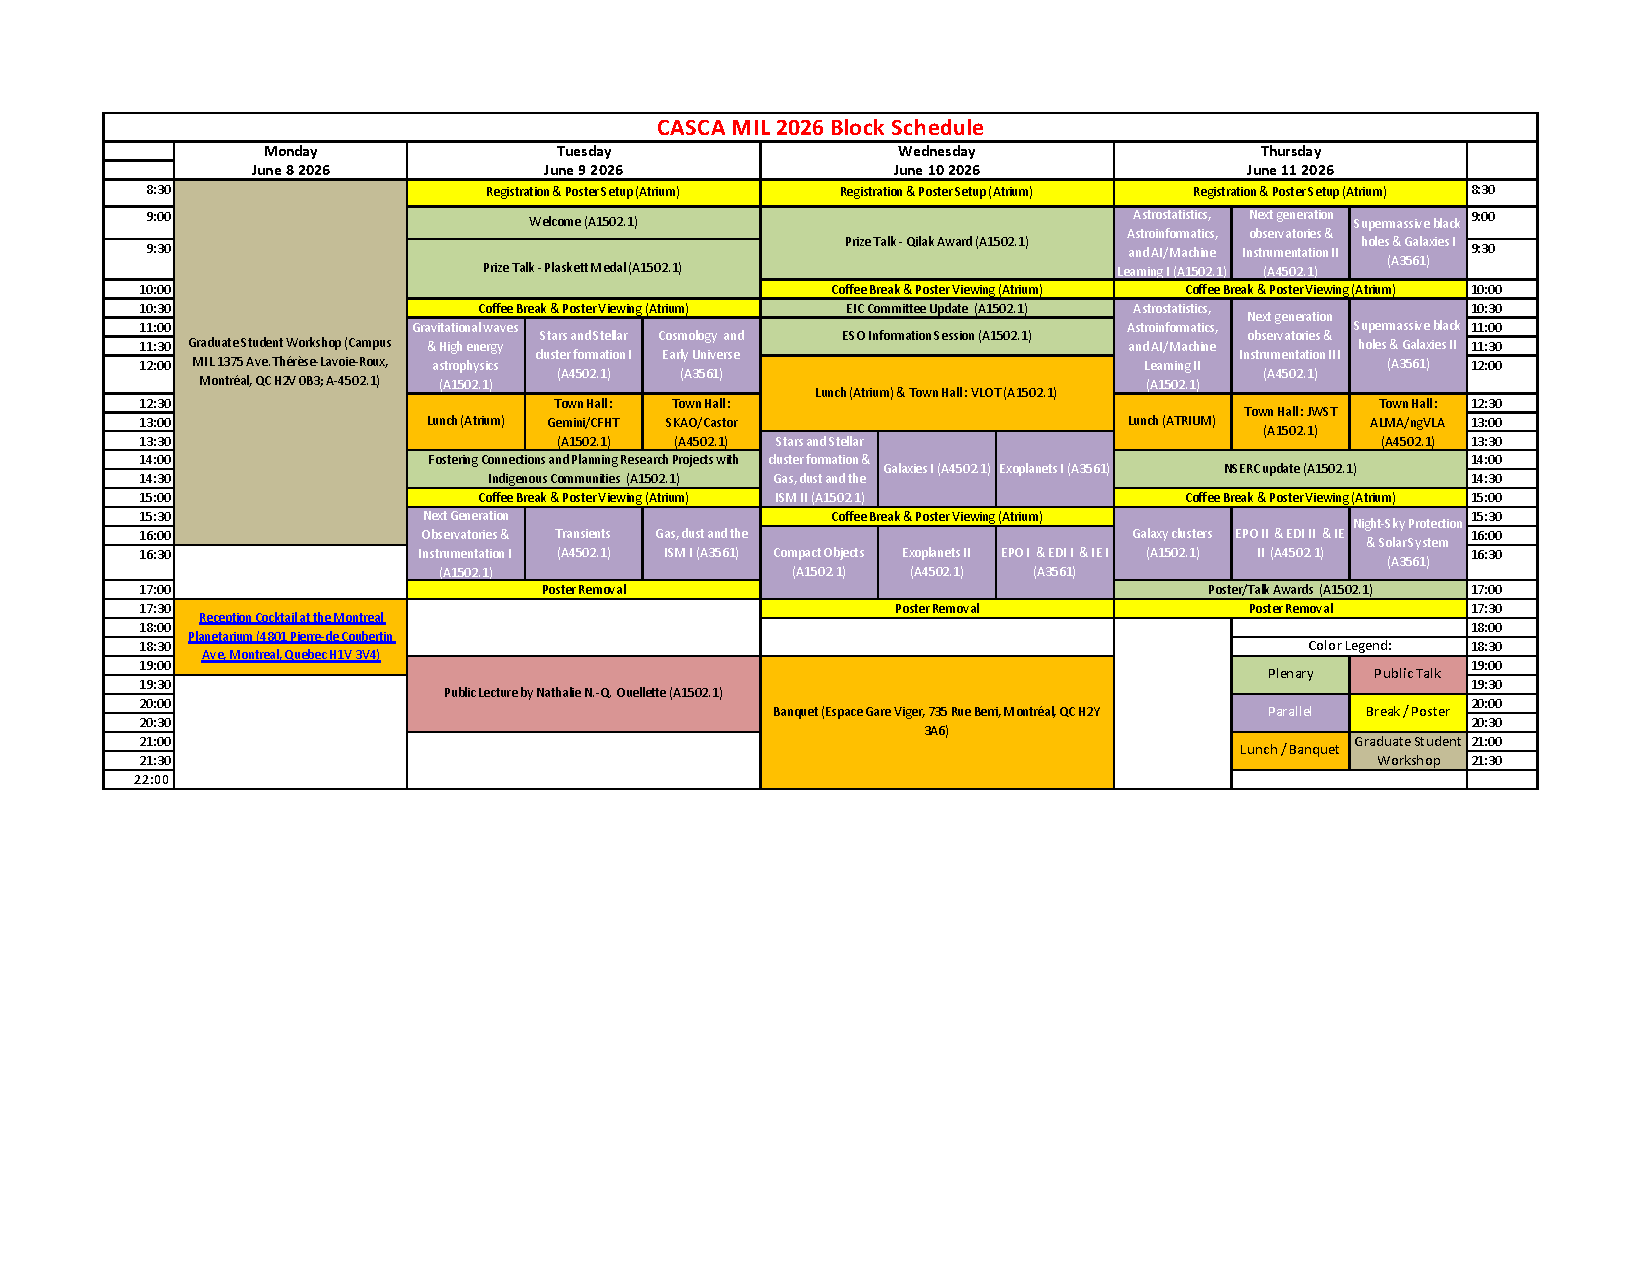
\includepdf[pages=-,fitpaper=true]{assets/block-en.pdf}
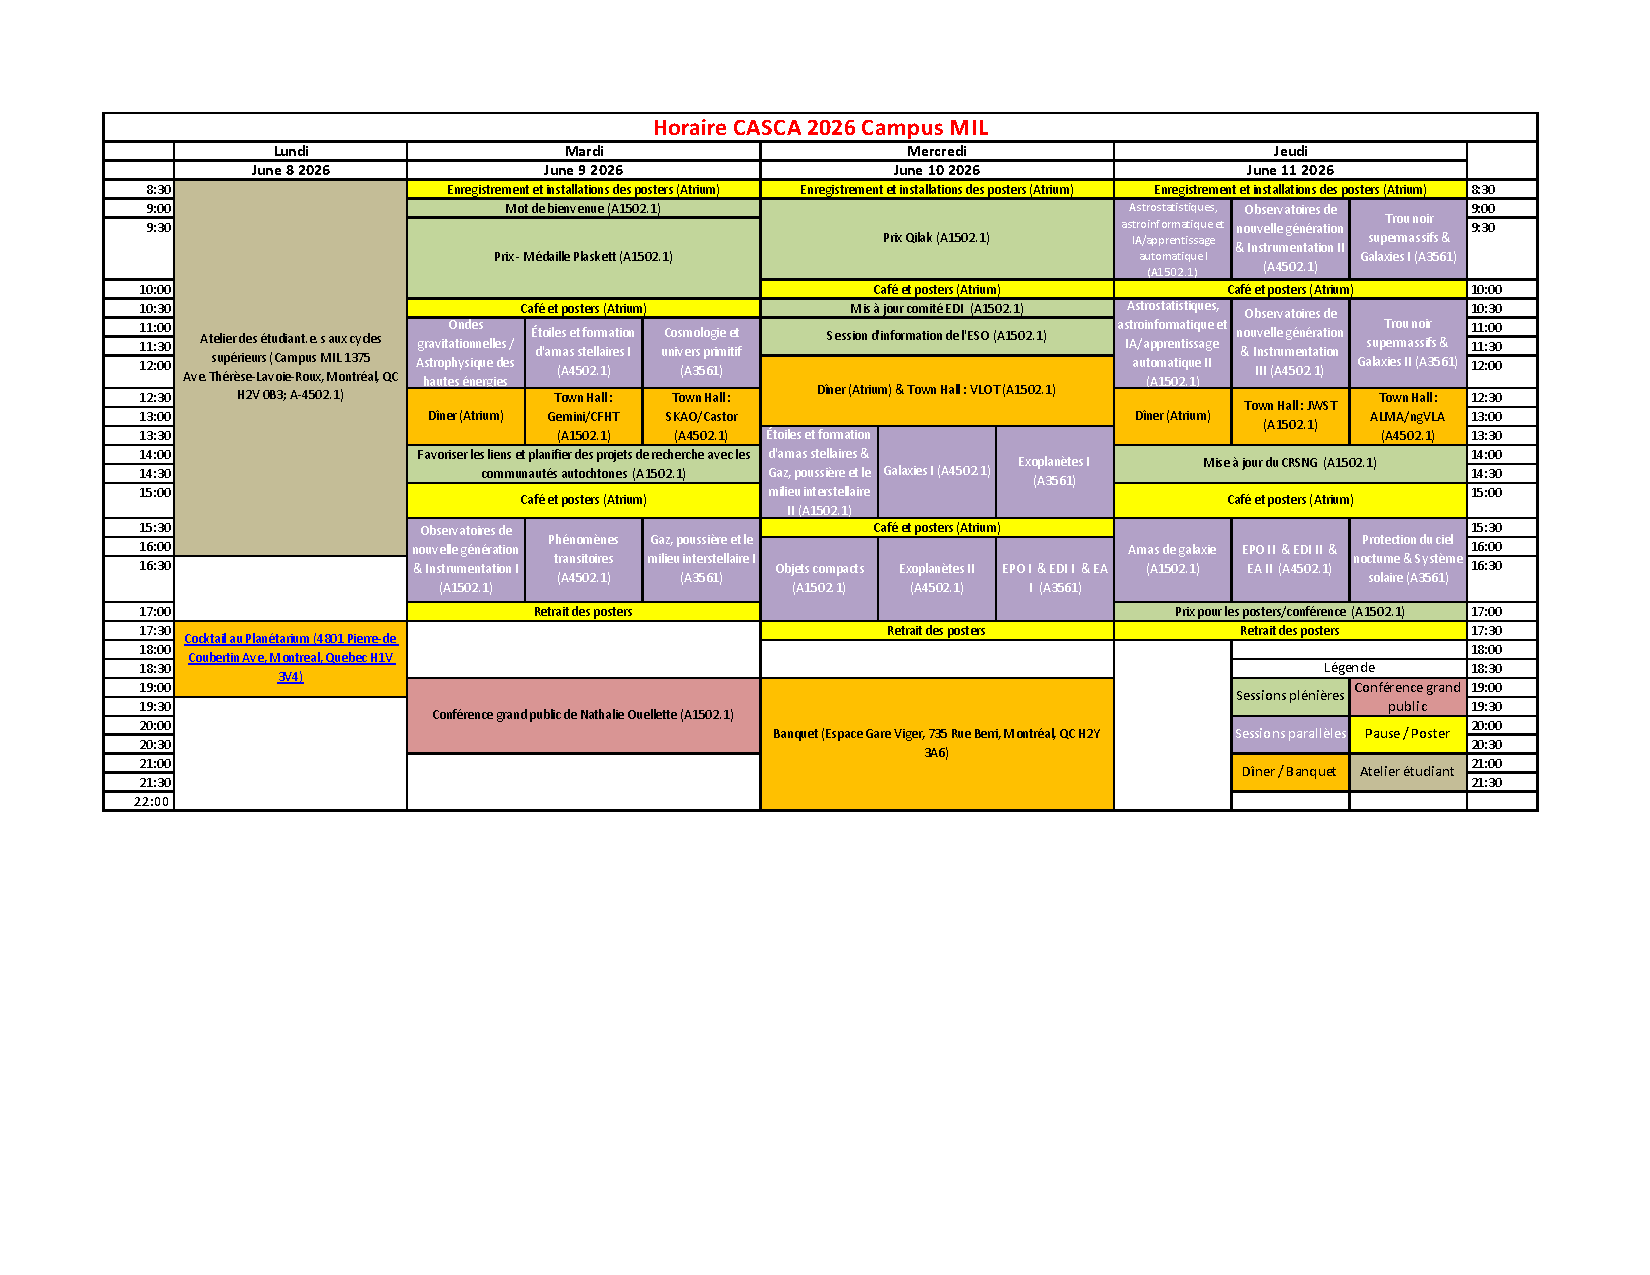
\includepdf[pages=-,fitpaper=true]{assets/block-fr.pdf}

\enableinsideastrobackground

\pagenumbering{roman}
\hypertarget{nav-overview}{}
\section*{Conference At a Glance}
\addcontentsline{toc}{section}{Conference At a Glance}
{\small\color{deepviolet} Use these opening pages for a quick route through the meeting, then jump directly to the detailed sections later in the program.}

\begin{center}
\setlength{\tabcolsep}{6pt}
\renewcommand{\arraystretch}{1.0}
\begin{tabular}{ccc}
\hyperlink{nav-practical}{\fcolorbox{lightrule}{softpanel}{\begin{minipage}[c][6.0em][c]{0.28\textwidth}\centering\sffamily\bfseries\color{cascadeep} Practical Information\\[0.15em]{\small\normalfont\color{deepviolet} Campus map, wifi, childcare, and logistics}\\[0.2em]{\footnotesize\color{cascateal} p.~\pageref{nav-page-practical}}\end{minipage}}} & 
\hyperlink{nav-oral-schedule}{\fcolorbox{lightrule}{cascablue!10}{\begin{minipage}[c][6.0em][c]{0.28\textwidth}\centering\sffamily\bfseries\color{cascadeep} Conference Schedule\\[0.15em]{\small\normalfont\color{deepviolet} Detailed oral sessions by day and room}\\[0.2em]{\footnotesize\color{cascateal} p.~\pageref{nav-page-oral-schedule}}\end{minipage}}} & 
\hyperlink{nav-poster-schedule}{\fcolorbox{lightrule}{cascagold!16}{\begin{minipage}[c][6.0em][c]{0.28\textwidth}\centering\sffamily\bfseries\color{cascadeep} Poster Schedule\\[0.15em]{\small\normalfont\color{deepviolet} Poster assignments and daily boards}\\[0.2em]{\footnotesize\color{cascateal} p.~\pageref{nav-page-poster-schedule}}\end{minipage}}} \\[0.5em]
\hyperlink{invited-alan-knee}{\fcolorbox{lightrule}{auroraglow!18}{\begin{minipage}[c][6.0em][c]{0.28\textwidth}\centering\sffamily\bfseries\color{cascadeep} Invited Speakers\\[0.15em]{\small\normalfont\color{deepviolet} Prize and invited lecture section}\\[0.2em]{\footnotesize\color{cascateal} p.~\pageref{invited-page-alan-knee}}\end{minipage}}} & 
\hyperlink{nav-abstracts}{\fcolorbox{lightrule}{nebulaedge}{\begin{minipage}[c][6.0em][c]{0.28\textwidth}\centering\sffamily\bfseries\color{cascadeep} List of Abstracts\\[0.15em]{\small\normalfont\color{deepviolet} All contributed oral abstracts}\\[0.2em]{\footnotesize\color{cascateal} p.~\pageref{nav-page-abstracts}}\end{minipage}}} & 
\hyperlink{nav-poster-abstracts}{\fcolorbox{lightrule}{nebulaedge}{\begin{minipage}[c][6.0em][c]{0.28\textwidth}\centering\sffamily\bfseries\color{cascadeep} List of Poster Abstracts\\[0.15em]{\small\normalfont\color{deepviolet} All contributed poster abstracts}\\[0.2em]{\footnotesize\color{cascateal} p.~\pageref{nav-page-poster-abstracts}}\end{minipage}}}  
%\hyperlink{nav-title-index}{\fcolorbox{lightrule}{paperwarm}{\begin{minipage}[c][6.0em][c]{0.28\textwidth}\centering\sffamily\bfseries\color{cascadeep} Topic Index\\[0.15em]%{\small\normalfont\color{deepviolet} Talk and poster index by topic}\\[0.2em]{\footnotesize\color{cascateal} p.~\pageref{nav-page-title-index}}\end{minipage}}} \\[0.5em]
\end{tabular}
\end{center}

% Emit TOC entries directly, skipping the \chapter* that would add a blank page
\clearpage
{\noindent\color{deepviolet}\rule{\textwidth}{1.2pt}\par\vspace{0.6em}}
{\sffamily\bfseries\Large\color{cascablue} Table of Contents\par}
\vspace{0.8em}
\makeatletter\@starttoc{toc}\makeatother
\clearpage

\programchapter{Local Organizing Committee}
\begin{multicols}{2}
\begin{itemize}
  \item Fr\'ed\'erique Baron (chair)
  \item Julie Hlavacek-Larrondo (co-chair)
  \item Ren\'e Doyon (co-chair)
  \item Loic Albert (secretary)
  \item \'Etienne Artigau
  \item Lison Malo
  \item Olivier Hernandez
  \item \'Erika Le Bourdais
  \item Mathieu Marquis
  \item Nathalie Ouellette
  \item Sacha Perry-Fagant
  \item Olivia Pereira
  \item Anabel Q. Tan
  \item Auriane Thilloy
  \item Benjamin Vigneron
  \item Marek Detière-Venkatesh
\end{itemize}
\end{multicols}
\bigskip
{\large\bfseries\sffamily Scientific Organizing Committee}
\addcontentsline{toc}{chapter}{Scientific Organizing Committee}
\markboth{Scientific Organizing Committee}{Scientific Organizing Committee}
\begin{multicols}{2}
\begin{itemize}
  \item Julie Hlavacek-Larrondo (co-chair)
  \item Ren\'e Doyon (co-chair)
  \item \'Etienne Artigau
  \item Cassandra Bolduc
  \item Toby Brown
  \item Andr\'e-Nicholas Chen\'e
  \item Lisa Dang
  \item Gwen Eadie
  \item Jonathan Gagn\'e
  \item Luigi Gallo
  \item Michele Kunimoto
  \item Allison Man
  \item Sharon Morsink
  \item Laurence Perreault-Levasseur
  \item Samar Safi-Harb
\end{itemize}
\end{multicols}
\programchapter{List of Participants}
\begin{small}
\setlength{\columnsep}{1.5em}
\begin{multicols}{2}
\raggedright
\setlength{\parskip}{1.5pt}
\setlength{\parindent}{0pt}

{\sffamily\bfseries\color{cascablue}\large A}\\[2pt]

\textbf{Abhilash, Sharone}, {\footnotesize\textit{University of Toronto}}\par
\textbf{Agrawal, Mohan}, {\footnotesize\textit{McGill University}} \hyperref[abstract-page-talk-200]{\scriptsize\textcolor{cascablue}{[Talk]}}\par
\textbf{Ahad, Syeda Lammim}, {\footnotesize\textit{Waterloo Centre for Astrophysics}} \hyperref[poster-abstract-page-talk-152]{\scriptsize\textcolor{cascateal}{[Poster]}}\par
\textbf{Allart, Romain}, {\footnotesize\textit{Université de Montréal}} \hyperref[abstract-page-talk-234]{\scriptsize\textcolor{cascablue}{[Talk]}}\par
\textbf{Amen, Laurie}, {\footnotesize\textit{McGill University}}\par
\textbf{Amouyal, Daniel}, {\footnotesize\textit{McGill University}} \hyperref[poster-abstract-page-talk-96]{\scriptsize\textcolor{cascateal}{[Poster]}}\par
\textbf{Ansdell, Megan}, {\footnotesize\textit{NASA HQ}}\par
\textbf{Armstrong, Isabella}, {\footnotesize\textit{McMaster University}} \hyperref[poster-abstract-page-talk-50]{\scriptsize\textcolor{cascateal}{[Poster]}}\par
\textbf{Arora, Nikhil}, {\footnotesize\textit{Arthur B. McDonald Canadian Astroparticle Physics Research Institute}}\par
\textbf{Artigau, Étienne}, {\footnotesize\textit{Université de Montréal}}\par
\textbf{Ashok, Aayushmathi}, {\footnotesize\textit{Graduate Student, Department of Physics and Astronomy, University of Victoria}} \hyperref[poster-abstract-page-talk-143]{\scriptsize\textcolor{cascateal}{[Poster]}}\par
\textbf{Atwood, Jenny}, {\footnotesize\textit{National Research Council Herzberg Astronomy and Astrophysics}}\par

{\sffamily\bfseries\color{cascablue}\large B}\\[2pt]

\textbf{Babic, Sara}, {\footnotesize\textit{Bishop's University}} \hyperref[poster-abstract-page-talk-206]{\scriptsize\textcolor{cascateal}{[Poster]}}\par
\textbf{Bagchi, Mayukh}, {\footnotesize\textit{Queen's University}} \hyperref[poster-abstract-page-talk-63]{\scriptsize\textcolor{cascateal}{[Poster]}}\par
\textbf{Balakrishnan, Mayura}, {\footnotesize\textit{McGill University}} \hyperref[abstract-page-talk-13]{\scriptsize\textcolor{cascablue}{[Talk]}} \hyperref[poster-abstract-page-talk-123]{\scriptsize\textcolor{cascateal}{[Poster]}}\par
\textbf{Ball, Brianna}, {\footnotesize\textit{University of Alberta}} \hyperref[poster-abstract-page-talk-47]{\scriptsize\textcolor{cascateal}{[Poster]}}\par
\textbf{Balogh, Michael}, {\footnotesize\textit{University of Waterloo}} \hyperref[abstract-page-talk-82]{\scriptsize\textcolor{cascablue}{[Talk]}}\par
\textbf{Barco, Gabriel Missael}, {\footnotesize\textit{Université de Montréal}} \hyperref[abstract-page-talk-317]{\scriptsize\textcolor{cascablue}{[Talk]}}\par
\textbf{Bardwell, Joe}, {\footnotesize\textit{University of Alberta}}\par
\textbf{Baron, Frédérique}, {\footnotesize\textit{Université de Montréal}}\par
\textbf{Barré, Ruxin}, {\footnotesize\textit{University of Victoria}} \hyperref[abstract-page-talk-29]{\scriptsize\textcolor{cascablue}{[Talk]}}\par
\textbf{Barrera Ballesteros, Jorge Karolt}, {\footnotesize\textit{Université de Montreal}}\par
\textbf{Barron, James}, {\footnotesize\textit{Queen's University}} \hyperref[abstract-page-talk-121]{\scriptsize\textcolor{cascablue}{[Talk]}}\par
\textbf{Barth, Michael}, {\footnotesize\textit{University of Montreal}}\par
\textbf{Bastien, Pierre}, {\footnotesize\textit{Université de Montréal}}\par
\textbf{Beaulieu, Sylvie F}, {\footnotesize\textit{Observatoire du Mont-Mégantic UdeM}}\par
\textbf{Bélanger, Flavie}, {\footnotesize\textit{Université de Montréal}}\par
\textbf{Belzile, Danika}, {\footnotesize\textit{Université de Montréal}}\par
\textbf{Berek, Samantha}, {\footnotesize\textit{University of Massachusetts, Amherst}}\par
\textbf{Bernier, Audréanne (Audrey)}, {\footnotesize\textit{McGill University}}\par
\textbf{Bhangal, Joe}, {\footnotesize\textit{University of British Columbia}} \hyperref[abstract-page-talk-136]{\scriptsize\textcolor{cascablue}{[Talk]}}\par
\textbf{Bhatt, Charmi}, {\footnotesize\textit{Western University}} \hyperref[abstract-page-talk-326]{\scriptsize\textcolor{cascablue}{[Talk]}}\par
\textbf{Blakely, Dori}, {\footnotesize\textit{University of Victoria}} \hyperref[abstract-page-talk-31]{\scriptsize\textcolor{cascablue}{[Talk]}}\par
\textbf{Blamart, Mattéo}, {\footnotesize\textit{McGill University}} \hyperref[abstract-page-talk-251]{\scriptsize\textcolor{cascablue}{[Talk]}}\par
\textbf{Bolduc, Cassandra}, {\footnotesize\textit{Canadian Space Agency}}\par
\textbf{Bolduc-Duval, Julie}, {\footnotesize\textit{Discover the Universe / À la découverte de l'univers}}\par
\textbf{Boley, Aaron}, {\footnotesize\textit{University of British Columbia}} \hyperref[abstract-page-talk-305]{\scriptsize\textcolor{cascablue}{[Talk]}} \hyperref[poster-abstract-page-talk-303]{\scriptsize\textcolor{cascateal}{[Poster]}}\par
\textbf{Bosch-Cabot, Pau}, {\footnotesize\textit{University of Lethbridge}} \hyperref[poster-abstract-page-talk-36]{\scriptsize\textcolor{cascateal}{[Poster]}}\par
\textbf{Boucher, Samuel}, {\footnotesize\textit{Université de Montréal}} \hyperref[poster-abstract-page-talk-237]{\scriptsize\textcolor{cascateal}{[Poster]}}\par
\textbf{Bouffard, Mathis}, {\footnotesize\textit{Université de Montréal}} \hyperref[poster-abstract-page-talk-53]{\scriptsize\textcolor{cascateal}{[Poster]}}\par
\textbf{Boukaré, Charles-Édouard}, {\footnotesize\textit{York University}}\par
\textbf{Brandt, Kieron}, {\footnotesize\textit{McGill University}}\par
\textbf{Brousseau, Denis}, {\footnotesize\textit{Université Laval}} \hyperref[poster-abstract-page-talk-219]{\scriptsize\textcolor{cascateal}{[Poster]}}\par
\textbf{Buchanan, Laura}, {\footnotesize\textit{University of Victoria}} \hyperref[abstract-page-talk-244]{\scriptsize\textcolor{cascablue}{[Talk]}}\par
\textbf{Budz, Noah}, {\footnotesize\textit{Queen's University}} \hyperref[poster-abstract-page-talk-190]{\scriptsize\textcolor{cascateal}{[Poster]}}\par
\textbf{Burggraf, Audrey}, {\footnotesize\textit{Queen's University}} \hyperref[poster-abstract-page-talk-302]{\scriptsize\textcolor{cascateal}{[Poster]}}\par

{\sffamily\bfseries\color{cascablue}\large C}\\[2pt]

\textbf{Carlson, Nathan J.}, {\footnotesize\textit{University of Toronto/CITA}} \hyperref[abstract-page-talk-293]{\scriptsize\textcolor{cascablue}{[Talk]}}\par
\textbf{Carver, Emily}, {\footnotesize\textit{University of Lethbridge}} \hyperref[poster-abstract-page-talk-207]{\scriptsize\textcolor{cascateal}{[Poster]}}\par
\textbf{Cassity, Alyssa}, {\footnotesize\textit{The University of British Columbia}} \hyperref[poster-abstract-page-talk-277]{\scriptsize\textcolor{cascateal}{[Poster]}}\par
\textbf{Castro-Tapia, Matias}, {\footnotesize\textit{McGill University}} \hyperref[abstract-page-talk-137]{\scriptsize\textcolor{cascablue}{[Talk]}}\par
\textbf{Caza, Julian}, {\footnotesize\textit{Queen's University}} \hyperref[poster-abstract-page-talk-89]{\scriptsize\textcolor{cascateal}{[Poster]}}\par
\textbf{Chamma, Mohammed}, {\footnotesize\textit{McGill University}} \hyperref[abstract-page-talk-140]{\scriptsize\textcolor{cascablue}{[Talk]}}\par
\textbf{Charbonneau, Paul}, {\footnotesize\textit{Université de Montréal}}\par
\textbf{Chastenay, Pierre}, {\footnotesize\textit{Université du Québec à Montréal}} \hyperref[abstract-page-talk-3]{\scriptsize\textcolor{cascablue}{[Talk]}}\par
\textbf{Chené, André-Nicolas}, {\footnotesize\textit{NSF NOIRLab}} \hyperref[poster-abstract-page-talk-286]{\scriptsize\textcolor{cascateal}{[Poster]}}\par
\textbf{Cheung, Benjamin}, {\footnotesize\textit{McMaster University}} \hyperref[abstract-page-talk-260]{\scriptsize\textcolor{cascablue}{[Talk]}}\par
\textbf{Choi, Woorak}, {\footnotesize\textit{McMaster University}} \hyperref[abstract-page-talk-160]{\scriptsize\textcolor{cascablue}{[Talk]}}\par
\textbf{Choudhuri, Aradhana}, {\footnotesize\textit{Honeywell Aerospace Canada (Com Dev)}}\par
\textbf{Christie, Scott}, {\footnotesize\textit{Dunlap Institute - University of Toronto}}\par
\textbf{Cichonski, Mike}, {\footnotesize\textit{CanDIAPL}}\par
\textbf{Clark, Nicholas}, {\footnotesize\textit{Western University}} \hyperref[abstract-page-talk-113]{\scriptsize\textcolor{cascablue}{[Talk]}}\par
\textbf{Cloutier, Ryan}, {\footnotesize\textit{McMaster University}} \hyperref[abstract-page-talk-28]{\scriptsize\textcolor{cascablue}{[Talk]}}\par
\textbf{Concha-Marroquin, Nicolas}, {\footnotesize\textit{University of Alberta}} \hyperref[poster-abstract-page-talk-141]{\scriptsize\textcolor{cascateal}{[Poster]}}\par
\textbf{Connors, Martin}, {\footnotesize\textit{Athabasca University/UCLA}} \hyperref[poster-abstract-page-talk-270]{\scriptsize\textcolor{cascateal}{[Poster]}}\par
\textbf{Connors, Nicholas}, {\footnotesize\textit{Waterloo University}} \hyperref[poster-abstract-page-talk-312]{\scriptsize\textcolor{cascateal}{[Poster]}}\par
\textbf{Cook, Neil}, {\footnotesize\textit{Universite de Montreal}} \hyperref[poster-abstract-page-talk-105]{\scriptsize\textcolor{cascateal}{[Poster]}}\par
\textbf{Cordeiro de Almeida, Toni}, {\footnotesize\textit{University of Western Ontario}} \hyperref[abstract-page-talk-265]{\scriptsize\textcolor{cascablue}{[Talk]}}\par
\textbf{Cote, Patrick}, {\footnotesize\textit{National Research Council of Canada, Herzberg Astronomy \& Astrophysics Research Centre}}\par
\textbf{Coulombe, Louis-Philippe}, {\footnotesize\textit{Planétarium de Montréal}} \hyperref[poster-abstract-page-talk-56]{\scriptsize\textcolor{cascateal}{[Poster]}}\par
\textbf{Cowan, Kristen}, {\footnotesize\textit{Saint Mary's University}}\par
\textbf{Cowan, Nicolas}, {\footnotesize\textit{McGill}}\par
\textbf{Cruz-Vinaccia, Carolina}, {\footnotesize\textit{McGill University, Department of Integrated Studies in Education}} \hyperref[abstract-page-talk-310]{\scriptsize\textcolor{cascablue}{[Talk]}}\par
\textbf{Curtin, Alice}, {\footnotesize\textit{McGill University}} \hyperref[abstract-page-talk-134]{\scriptsize\textcolor{cascablue}{[Talk]}}\par

{\sffamily\bfseries\color{cascablue}\large D}\\[2pt]

\textbf{D'Aoust, Lina}, {\footnotesize\textit{University of Waterloo}} \hyperref[poster-abstract-page-talk-261]{\scriptsize\textcolor{cascateal}{[Poster]}}\par
\textbf{da Conceicao, Lucas}, {\footnotesize\textit{University of Manitoba}} \hyperref[abstract-page-talk-283]{\scriptsize\textcolor{cascablue}{[Talk]}}\par
\textbf{Dahale, Rohan}, {\footnotesize\textit{University of Toronto}} \hyperref[abstract-page-talk-19]{\scriptsize\textcolor{cascablue}{[Talk]}}\par
\textbf{Daigle, Olivier}, {\footnotesize\textit{Nuvu Cameras}}\par
\textbf{Daigneault, Rafael}, {\footnotesize\textit{Université de Montréal}}\par
\textbf{Damjanov, Ivana}, {\footnotesize\textit{Saint Mary's University}} \hyperref[abstract-page-talk-329]{\scriptsize\textcolor{cascablue}{[Talk]}}\par
\textbf{Dang, Lisa}, {\footnotesize\textit{University of Waterloo}}\par
\textbf{Daniels, Darya}, {\footnotesize\textit{University of British Columbia / working at IREx and Université de Montréal for summer}}\par
\textbf{Das Gupta, Eesha}, {\footnotesize\textit{Trottier Space Institute at McGill University}} \hyperref[poster-abstract-page-talk-109]{\scriptsize\textcolor{cascateal}{[Poster]}}\par
\textbf{David-Uraz, Alexandre}, {\footnotesize\textit{Trottier Space Institute/McGill University}} \hyperref[poster-abstract-page-talk-220]{\scriptsize\textcolor{cascateal}{[Poster]}}\par
\textbf{Deg, Nathan}, {\footnotesize\textit{Queen's University}} \hyperref[poster-abstract-page-talk-45]{\scriptsize\textcolor{cascateal}{[Poster]}}\par
\textbf{Deibert, Emily}, {\footnotesize\textit{University of Waterloo}} \hyperref[poster-abstract-page-talk-32]{\scriptsize\textcolor{cascateal}{[Poster]}} \hyperref[poster-abstract-page-talk-104]{\scriptsize\textcolor{cascateal}{[Poster]}}\par
\textbf{Del Rizzo, Dave}, {\footnotesize\textit{NRC-HAA}}\par
\textbf{Detière-Venkatesh, Marek}, {\footnotesize\textit{McGill University}} \hyperref[poster-abstract-page-talk-162]{\scriptsize\textcolor{cascateal}{[Poster]}}\par
\textbf{Devost, Daniel}, {\footnotesize\textit{Canada-France-Hawaii Telescope Corporation.}}\par
\textbf{Di Francesco, James}, {\footnotesize\textit{National Research Council of Canada}}\par
\textbf{Dia, Noé}, {\footnotesize\textit{Université de Montréal}}\par
\textbf{Difonzo, Antonio}, {\footnotesize\textit{Canadian Space Agency}}\par
\textbf{Dong, Fengqiu}, {\footnotesize\textit{NRC, York University}}\par
\textbf{Donovan Meyer, Jennifer}, {\footnotesize\textit{National Radio Astronomy Observatory (NRAO)}}\par
\textbf{Doyon, René}, {\footnotesize\textit{Université de Montréal}}\par
\textbf{Drout, Maria}, {\footnotesize\textit{University of Toronto}}\par
\textbf{Dubé, Robin}, {\footnotesize\textit{Agence spatiale canadienne}}\par
\textbf{Ducharme, Jade}, {\footnotesize\textit{Brown University}} \hyperref[poster-abstract-page-talk-87]{\scriptsize\textcolor{cascateal}{[Poster]}}\par
\textbf{Dufour, Patrick}, {\footnotesize\textit{Université de Montréal}}\par
\textbf{Dufresne, George}, {\footnotesize\textit{Dartmouth College}} \hyperref[abstract-page-talk-70]{\scriptsize\textcolor{cascablue}{[Talk]}}\par
\textbf{Dufresne, James C.}, {\footnotesize\textit{University of Waterloo}} \hyperref[poster-abstract-page-talk-71]{\scriptsize\textcolor{cascateal}{[Poster]}}\par
\textbf{Dumaguin, Janine}, {\footnotesize\textit{Canada-France-Hawai'i Telescope}}\par
\textbf{Dupuis, Jean}, {\footnotesize\textit{Agence spatiale canadienne}}\par

{\sffamily\bfseries\color{cascablue}\large E}\\[2pt]

\textbf{Eduardo, Marielle}, {\footnotesize\textit{University of Victoria}} \hyperref[abstract-page-talk-319]{\scriptsize\textcolor{cascablue}{[Talk]}}\par
\textbf{Egal, Auriane}, {\footnotesize\textit{Planétarium de Montréal / Western University}} \hyperref[abstract-page-talk-177]{\scriptsize\textcolor{cascablue}{[Talk]}} \hyperref[poster-abstract-page-talk-182]{\scriptsize\textcolor{cascateal}{[Poster]}}\par

{\sffamily\bfseries\color{cascablue}\large F}\\[2pt]

\textbf{Fabiani, Luca}, {\footnotesize\textit{Université de Montréal}} \hyperref[poster-abstract-page-talk-285]{\scriptsize\textcolor{cascateal}{[Poster]}}\par
\textbf{Fang, Ningyan}, {\footnotesize\textit{University of Western Ontario}} \hyperref[abstract-page-talk-161]{\scriptsize\textcolor{cascablue}{[Talk]}}\par
\textbf{Farah, Amanda}, {\footnotesize\textit{CITA}}\par
\textbf{Faria, Lawrence}, {\footnotesize\textit{Queen's University}} \hyperref[poster-abstract-page-talk-34]{\scriptsize\textcolor{cascateal}{[Poster]}}\par
\textbf{Fielder, Samuel}, {\footnotesize\textit{University of Victoria}} \hyperref[abstract-page-talk-328]{\scriptsize\textcolor{cascablue}{[Talk]}}\par
\textbf{Fields, Tiffany}, {\footnotesize\textit{Saint Mary's University}} \hyperref[poster-abstract-page-talk-115]{\scriptsize\textcolor{cascateal}{[Poster]}}\par
\textbf{Fine, Maxwell}, {\footnotesize\textit{Mcgill}} \hyperref[poster-abstract-page-talk-146]{\scriptsize\textcolor{cascateal}{[Poster]}}\par
\textbf{Fissel, Laura}, {\footnotesize\textit{Queen's University}}\par
\textbf{Fogal, Andre}, {\footnotesize\textit{University of Victoria}} \hyperref[poster-abstract-page-talk-287]{\scriptsize\textcolor{cascateal}{[Poster]}}\par
\textbf{Ford, Nicole}, {\footnotesize\textit{McGill University}} \hyperref[poster-abstract-page-talk-239]{\scriptsize\textcolor{cascateal}{[Poster]}}\par
\textbf{Fortier, Nickolas}, {\footnotesize\textit{University of Lethbridge}}\par
\textbf{Fraser, Wesley}, {\footnotesize\textit{Herzberg Astronomy and Astrophysics Research Centre}}\par
\textbf{Friesen, Rachel}, {\footnotesize\textit{University of Toronto}}\par
\textbf{Frisella, Nicolas}, {\footnotesize\textit{Western University}} \hyperref[poster-abstract-page-talk-185]{\scriptsize\textcolor{cascateal}{[Poster]}}\par
\textbf{Fronenberg, Hannah}, {\footnotesize\textit{University of Chicago}}\par

{\sffamily\bfseries\color{cascablue}\large G}\\[2pt]

\textbf{Gagné, Jonathan}, {\footnotesize\textit{Université de Montréal, Planétarium de Montréal}}\par
\textbf{Gallagher, Sarah}, {\footnotesize\textit{Western University}}\par
\textbf{Gendron-Marsolais, Marie-Lou}, {\footnotesize\textit{Université Laval}}\par
\textbf{Genest, Frédéric}, {\footnotesize\textit{Université de Montréal}} \hyperref[poster-abstract-page-talk-42]{\scriptsize\textcolor{cascateal}{[Poster]}}\par
\textbf{George, Angelo}, {\footnotesize\textit{ASIAA, Taipei and Saint Mary's University, Halifax}} \hyperref[abstract-page-talk-51]{\scriptsize\textcolor{cascablue}{[Talk]}}\par
\textbf{Ghodsi, Laya}, {\footnotesize\textit{University of British Columbia}} \hyperref[abstract-page-talk-145]{\scriptsize\textcolor{cascablue}{[Talk]}} \hyperref[poster-abstract-page-talk-297]{\scriptsize\textcolor{cascateal}{[Poster]}}\par
\textbf{Gingras, Marie-Joëlle}, {\footnotesize\textit{University of Waterloo, Waterloo Centre for Astrophysics}} \hyperref[abstract-page-talk-316]{\scriptsize\textcolor{cascablue}{[Talk]}}\par
\textbf{Glasman, Pénélope}, {\footnotesize\textit{Université Laval}} \hyperref[abstract-page-talk-101]{\scriptsize\textcolor{cascablue}{[Talk]}}\par
\textbf{Graham, Gabrielle}, {\footnotesize\textit{University of Alberta}} \hyperref[poster-abstract-page-talk-77]{\scriptsize\textcolor{cascateal}{[Poster]}}\par
\textbf{Grandmont, Frederic}, {\footnotesize\textit{ABB}}\par
\textbf{Gressier, Amélie}, {\footnotesize\textit{Université de Montréal}} \hyperref[abstract-page-talk-224]{\scriptsize\textcolor{cascablue}{[Talk]}}\par
\textbf{Grosdidier, Yves}, {\footnotesize\textit{Département de physique, Université de Sherbrooke}}\par
\textbf{Grosson, Theodore}, {\footnotesize\textit{University of Victoria}} \hyperref[poster-abstract-page-talk-148]{\scriptsize\textcolor{cascateal}{[Poster]}}\par
\textbf{Gu, Shiming}, {\footnotesize\textit{University of British Columbia}} \hyperref[abstract-page-talk-49]{\scriptsize\textcolor{cascablue}{[Talk]}}\par
\textbf{Guan, Yilun}, {\footnotesize\textit{University of Toronto}} \hyperref[poster-abstract-page-talk-44]{\scriptsize\textcolor{cascateal}{[Poster]}}\par
\textbf{Guerras, Alice}, {\footnotesize\textit{Western University}} \hyperref[poster-abstract-page-talk-199]{\scriptsize\textcolor{cascateal}{[Poster]}}\par
\textbf{Gwyn, Stephen}, {\footnotesize\textit{Canadian Astronomy Data Centre}}\par

{\sffamily\bfseries\color{cascablue}\large H}\\[2pt]

\textbf{Haggar, Roan}, {\footnotesize\textit{University of Waterloo}} \hyperref[abstract-page-talk-211]{\scriptsize\textcolor{cascablue}{[Talk]}} \hyperref[poster-abstract-page-talk-202]{\scriptsize\textcolor{cascateal}{[Poster]}}\par
\textbf{Haggard, Daryl}, {\footnotesize\textit{McGill University}} \hyperref[poster-abstract-page-talk-120]{\scriptsize\textcolor{cascateal}{[Poster]}}\par
\textbf{Haggarty-Beamish, Jaclyn}, {\footnotesize\textit{Canadian Space Agency}}\par
\textbf{Harries, Nicholas}, {\footnotesize\textit{University of Calgary}} \hyperref[poster-abstract-page-talk-282]{\scriptsize\textcolor{cascateal}{[Poster]}}\par
\textbf{Harrison, Lauren}, {\footnotesize\textit{University of Victoria}}\par
\textbf{Hassani, Hamid}, {\footnotesize\textit{University of Alberta}} \hyperref[poster-abstract-page-talk-252]{\scriptsize\textcolor{cascateal}{[Poster]}}\par
\textbf{Hayduk, Mackenzie}, {\footnotesize\textit{Saint Mary's University}} \hyperref[poster-abstract-page-talk-150]{\scriptsize\textcolor{cascateal}{[Poster]}}\par
\textbf{Heise, Tyler}, {\footnotesize\textit{University of Alberta}}\par
\textbf{Hélias, Adrien}, {\footnotesize\textit{Western University}} \hyperref[abstract-page-talk-193]{\scriptsize\textcolor{cascablue}{[Talk]}}\par
\textbf{Hénault-Brunet, Vincent}, {\footnotesize\textit{Saint Mary's University}}\par
\textbf{Hernandez, Olivier}, {\footnotesize\textit{Planétarium de Montréal}}\par
\textbf{Hessel, Kaitlyn}, {\footnotesize\textit{University of Victoria}} \hyperref[abstract-page-talk-194]{\scriptsize\textcolor{cascablue}{[Talk]}}\par
\textbf{Hill, Alexis}, {\footnotesize\textit{NRC Herzberg}}\par
\textbf{Hlavacek-Larrondo, Julie}, {\footnotesize\textit{Université de Montréal}}\par
\textbf{Hlozek, Renée}, {\footnotesize\textit{University of Toronto}}\par
\textbf{Hoffman, Kelsey}, {\footnotesize\textit{Bishop's University}} \hyperref[poster-abstract-page-talk-186]{\scriptsize\textcolor{cascateal}{[Poster]}}\par
\textbf{Hopkins, Hans}, {\footnotesize\textit{University of Waterloo}} \hyperref[poster-abstract-page-talk-40]{\scriptsize\textcolor{cascateal}{[Poster]}}\par
\textbf{Horlaville, Patrick}, {\footnotesize\textit{TSI, McGill University}} \hyperref[poster-abstract-page-talk-320]{\scriptsize\textcolor{cascateal}{[Poster]}}\par
\textbf{Huang, Jeff}, {\footnotesize\textit{McGill University}}\par
\textbf{Huang, Russell}, {\footnotesize\textit{Mountain View High School}} \hyperref[poster-abstract-page-talk-30]{\scriptsize\textcolor{cascateal}{[Poster]}}\par
\textbf{Huang, Vi}, {\footnotesize\textit{Cosmic Minds}}\par
\textbf{Hudson, Mike}, {\footnotesize\textit{Waterloo Centre for Astrophysics}} \hyperref[abstract-page-talk-176]{\scriptsize\textcolor{cascablue}{[Talk]}}\par
\textbf{Hunt, Qiana}, {\footnotesize\textit{University of Lethbridge}} \hyperref[abstract-page-talk-117]{\scriptsize\textcolor{cascablue}{[Talk]}}\par
\textbf{Hurley, Grant}, {\footnotesize\textit{Queen's University}} \hyperref[abstract-page-talk-180]{\scriptsize\textcolor{cascablue}{[Talk]}}\par

{\sffamily\bfseries\color{cascablue}\large I}\\[2pt]

\textbf{Irons, Raina}, {\footnotesize\textit{Queen's University}} \hyperref[poster-abstract-page-talk-331]{\scriptsize\textcolor{cascateal}{[Poster]}}\par

{\sffamily\bfseries\color{cascablue}\large J}\\[2pt]

\textbf{Jain, Naman}, {\footnotesize\textit{McGill University}} \hyperref[abstract-page-talk-33]{\scriptsize\textcolor{cascablue}{[Talk]}}\par
\textbf{Jarvis, Emma}, {\footnotesize\textit{University of Toronto}} \hyperref[abstract-page-talk-154]{\scriptsize\textcolor{cascablue}{[Talk]}}\par
\textbf{Jiang, Hansen}, {\footnotesize\textit{Sidrat Research}}\par
\textbf{Jiang, Nan}, {\footnotesize\textit{Univ. of Toronto}} \hyperref[abstract-page-talk-269]{\scriptsize\textcolor{cascablue}{[Talk]}}\par
\textbf{Johnstone, Doug}, {\footnotesize\textit{NRC-Herzberg Astronomy and Astrophysics}} \hyperref[abstract-page-talk-76]{\scriptsize\textcolor{cascablue}{[Talk]}}\par
\textbf{Joncas, Gilles}, {\footnotesize\textit{Université Laval}}\par
\textbf{Jones, Gareth}, {\footnotesize\textit{University of Manitoba}} \hyperref[poster-abstract-page-talk-212]{\scriptsize\textcolor{cascateal}{[Poster]}}\par
\textbf{Juneau, Stéphanie}, {\footnotesize\textit{NSF NOIRLab}} \hyperref[poster-abstract-page-talk-294]{\scriptsize\textcolor{cascateal}{[Poster]}} \hyperref[poster-abstract-page-talk-334]{\scriptsize\textcolor{cascateal}{[Poster]}}\par

{\sffamily\bfseries\color{cascablue}\large K}\\[2pt]

\textbf{Kafando, Issouf}, {\footnotesize\textit{Collège Militaire Royal du Canada}}\par
\textbf{Kaushal, Ishan}, {\footnotesize\textit{Memorial University of Newfoundland}} \hyperref[poster-abstract-page-talk-276]{\scriptsize\textcolor{cascateal}{[Poster]}}\par
\textbf{Kerr, Ronan}, {\footnotesize\textit{University of Toronto}} \hyperref[poster-abstract-page-talk-58]{\scriptsize\textcolor{cascateal}{[Poster]}}\par
\textbf{Khadir, Affan}, {\footnotesize\textit{McGill University}} \hyperref[poster-abstract-page-talk-98]{\scriptsize\textcolor{cascateal}{[Poster]}}\par
\textbf{Khadour, Zayna}, {\footnotesize\textit{McMaster University}} \hyperref[poster-abstract-page-talk-39]{\scriptsize\textcolor{cascateal}{[Poster]}}\par
\textbf{Khalack, Viktor}, {\footnotesize\textit{Université de Moncton}} \hyperref[poster-abstract-page-talk-81]{\scriptsize\textcolor{cascateal}{[Poster]}}\par
\textbf{Khamar, Chaitanya}, {\footnotesize\textit{CITA-University of Toronto}} \hyperref[abstract-page-talk-307]{\scriptsize\textcolor{cascablue}{[Talk]}}\par
\textbf{Khatu, Viraja}, {\footnotesize\textit{Canada-France-Hawaii Telescope Corporation}} \hyperref[poster-abstract-page-talk-295]{\scriptsize\textcolor{cascateal}{[Poster]}} \hyperref[poster-abstract-page-talk-325]{\scriptsize\textcolor{cascateal}{[Poster]}}\par
\textbf{Khullar, Dev}, {\footnotesize\textit{University of Lethbridge}} \hyperref[poster-abstract-page-talk-107]{\scriptsize\textcolor{cascateal}{[Poster]}}\par
\textbf{Kim, Jinoo}, {\footnotesize\textit{McMaster University}} \hyperref[poster-abstract-page-talk-130]{\scriptsize\textcolor{cascateal}{[Poster]}}\par
\textbf{Knee, Alan}, {\footnotesize\textit{University of Michigan}}\par
\textbf{Knee, Lewis}, {\footnotesize\textit{NRC-HAA}}\par
\textbf{Knowlton, Peter}, {\footnotesize\textit{University of Victoria}} \hyperref[poster-abstract-page-talk-271]{\scriptsize\textcolor{cascateal}{[Poster]}}\par
\textbf{Kothes, Roland}, {\footnotesize\textit{National Research Council Canada}} \hyperref[poster-abstract-page-talk-318]{\scriptsize\textcolor{cascateal}{[Poster]}}\par
\textbf{Kuenkel, Lars}, {\footnotesize\textit{McGill University}}\par
\textbf{Kumar, Rohan}, {\footnotesize\textit{McMaster University}} \hyperref[poster-abstract-page-talk-102]{\scriptsize\textcolor{cascateal}{[Poster]}}\par
\textbf{Kunimoto, Michelle}, {\footnotesize\textit{University of British Columbia}}\par

{\sffamily\bfseries\color{cascablue}\large L}\\[2pt]

\textbf{L'Heureux, Alexandrine}, {\footnotesize\textit{Université de Montréal - IREx}} \hyperref[abstract-page-talk-167]{\scriptsize\textcolor{cascablue}{[Talk]}}\par
\textbf{Lafrenière, David}, {\footnotesize\textit{Université de Montréal}}\par
\textbf{Laing, Isabelle}, {\footnotesize\textit{University of Toronto}}\par
\textbf{Laing, Jennifer}, {\footnotesize\textit{McMaster University}} \hyperref[poster-abstract-page-talk-197]{\scriptsize\textcolor{cascateal}{[Poster]}}\par
\textbf{Lambier, Samantha}, {\footnotesize\textit{Western University}} \hyperref[poster-abstract-page-talk-79]{\scriptsize\textcolor{cascateal}{[Poster]}}\par
\textbf{Lammert, Owen}, {\footnotesize\textit{University of Waterloo}} \hyperref[poster-abstract-page-talk-232]{\scriptsize\textcolor{cascateal}{[Poster]}}\par
\textbf{Langlois, Pierre}, {\footnotesize\textit{Agence Spatiale Canadienne}}\par
\textbf{Larivière, Maude}, {\footnotesize\textit{UBC/TRIUMF}} \hyperref[poster-abstract-page-talk-324]{\scriptsize\textcolor{cascateal}{[Poster]}}\par
\textbf{Lau, Mason}, {\footnotesize\textit{University of Waterloo}}\par
\textbf{Laverde Villarreal, Edwin}, {\footnotesize\textit{McMaster University}} \hyperref[poster-abstract-page-talk-65]{\scriptsize\textcolor{cascateal}{[Poster]}}\par
\textbf{Lawler, Sam}, {\footnotesize\textit{University of Regina}}\par
\textbf{Lazda, Mattias}, {\footnotesize\textit{University of Toronto}} \hyperref[poster-abstract-page-talk-191]{\scriptsize\textcolor{cascateal}{[Poster]}}\par
\textbf{Le Bourdais, Érika}, {\footnotesize\textit{Université de Montréal - Institut Trottier de recherche sur les exoplanètes}} \hyperref[abstract-page-talk-26]{\scriptsize\textcolor{cascablue}{[Talk]}}\par
\textbf{Leclerc, Élise}, {\footnotesize\textit{McGill University}} \hyperref[poster-abstract-page-talk-299]{\scriptsize\textcolor{cascateal}{[Poster]}}\par
\textbf{Ledger, Blake}, {\footnotesize\textit{University of Victoria}} \hyperref[abstract-page-talk-222]{\scriptsize\textcolor{cascablue}{[Talk]}}\par
\textbf{Lee, Charles}, {\footnotesize\textit{University of Manitoba}} \hyperref[poster-abstract-page-talk-263]{\scriptsize\textcolor{cascateal}{[Poster]}}\par
\textbf{Lee, Stephanie}, {\footnotesize\textit{University of Toronto}} \hyperref[poster-abstract-page-talk-309]{\scriptsize\textcolor{cascateal}{[Poster]}}\par
\textbf{Lei, Han}, {\footnotesize\textit{McGill University}} \hyperref[poster-abstract-page-talk-189]{\scriptsize\textcolor{cascateal}{[Poster]}}\par
\textbf{Lenoir-Craig, Guillaume}, {\footnotesize\textit{Université de Montréal}} \hyperref[poster-abstract-page-talk-308]{\scriptsize\textcolor{cascateal}{[Poster]}}\par
\textbf{Lérat, Matthieu}, {\footnotesize\textit{Université de Montréal}}\par
\textbf{Lévesque, Michaël}, {\footnotesize\textit{Université de Montréal}}\par
\textbf{Li, Andrew}, {\footnotesize\textit{University of Victoria}} \hyperref[poster-abstract-page-talk-338]{\scriptsize\textcolor{cascateal}{[Poster]}}\par
\textbf{Liang, Rosalind}, {\footnotesize\textit{University of Victoria}}\par
\textbf{Limoges, Marie-Michèle}, {\footnotesize\textit{Cosmodôme}}\par
\textbf{Liu, Adrian}, {\footnotesize\textit{McGill University}}\par
\textbf{Lizotte, Dereck-Alexandre}, {\footnotesize\textit{Université de Montréal}}\par
\textbf{Loney, Alyson}, {\footnotesize\textit{University of Western Ontario}} \hyperref[poster-abstract-page-talk-179]{\scriptsize\textcolor{cascateal}{[Poster]}}\par
\textbf{Long, Alexander}, {\footnotesize\textit{Cosmographic Software}}\par
\textbf{Lu, Anan}, {\footnotesize\textit{University of British Columbia}} \hyperref[poster-abstract-page-talk-122]{\scriptsize\textcolor{cascateal}{[Poster]}}\par
\textbf{Lussier, Danielle}, {\footnotesize\textit{Queen's University}} \hyperref[abstract-page-talk-55]{\scriptsize\textcolor{cascablue}{[Talk]}}\par

{\sffamily\bfseries\color{cascablue}\large M}\\[2pt]

\textbf{Main, Robert}, {\footnotesize\textit{McGill University}} \hyperref[poster-abstract-page-talk-209]{\scriptsize\textcolor{cascateal}{[Poster]}}\par
\textbf{Majidi, Fereshteh}, {\footnotesize\textit{UBC}} \hyperref[abstract-page-talk-22]{\scriptsize\textcolor{cascablue}{[Talk]}}\par
\textbf{Malo, Lison}, {\footnotesize\textit{Université de Montréal / Observatoire du Mont-Mégantic}} \hyperref[abstract-page-talk-172]{\scriptsize\textcolor{cascablue}{[Talk]}}\par
\textbf{Mann, Christopher}, {\footnotesize\textit{NRC-HAA}} \hyperref[poster-abstract-page-talk-90]{\scriptsize\textcolor{cascateal}{[Poster]}}\par
\textbf{Manojh, Bhuvan}, {\footnotesize\textit{McGill University}} \hyperref[poster-abstract-page-talk-225]{\scriptsize\textcolor{cascateal}{[Poster]}}\par
\textbf{Manset, Nadine}, {\footnotesize\textit{Canada-France-Hawaii Telescope}} \hyperref[abstract-page-talk-157]{\scriptsize\textcolor{cascablue}{[Talk]}} \hyperref[poster-abstract-page-talk-155]{\scriptsize\textcolor{cascateal}{[Poster]}}\par
\textbf{Marois, Christian}, {\footnotesize\textit{National Research Council of Canada}} \hyperref[poster-abstract-page-talk-218]{\scriptsize\textcolor{cascateal}{[Poster]}}\par
\textbf{Marquis, Mathieu}, {\footnotesize\textit{Université de Montréal}} \hyperref[abstract-page-talk-273]{\scriptsize\textcolor{cascablue}{[Talk]}}\par
\textbf{Martin, Thomas}, {\footnotesize\textit{Cégep Garneau et Université Laval}} \hyperref[poster-abstract-page-talk-195]{\scriptsize\textcolor{cascateal}{[Poster]}}\par
\textbf{Martinez, Diego}, {\footnotesize\textit{University of Waterloo}}\par
\textbf{Martorella, Natalia}, {\footnotesize\textit{McGill University}}\par
\textbf{Matesic, Michael}, {\footnotesize\textit{University of Montreal}}\par
\textbf{Matthews, Brenda}, {\footnotesize\textit{NRC Herzberg}} \hyperref[poster-abstract-page-talk-17]{\scriptsize\textcolor{cascateal}{[Poster]}}\par
\textbf{Matvei, Artiom}, {\footnotesize\textit{Université de Montréal}} \hyperref[abstract-page-talk-335]{\scriptsize\textcolor{cascablue}{[Talk]}} \hyperref[abstract-page-talk-335]{\scriptsize\textcolor{cascablue}{[Talk]}}\par
\textbf{Matzner, Christopher}, {\footnotesize\textit{University of Toronto}} \hyperref[poster-abstract-page-talk-192]{\scriptsize\textcolor{cascateal}{[Poster]}}\par
\textbf{McConnachie, Alan}, {\footnotesize\textit{NRC Herzberg}} \hyperref[abstract-page-talk-151]{\scriptsize\textcolor{cascablue}{[Talk]}}\par
\textbf{McCutcheon, Bill}, {\footnotesize\textit{University of B.C.}}\par
\textbf{McGee, Francis}, {\footnotesize\textit{McGill}} \hyperref[poster-abstract-page-talk-214]{\scriptsize\textcolor{cascateal}{[Poster]}}\par
\textbf{McGregor, Kyle}, {\footnotesize\textit{McGill University}} \hyperref[abstract-page-talk-227]{\scriptsize\textcolor{cascablue}{[Talk]}}\par
\textbf{McIver, Jess}, {\footnotesize\textit{UBC}}\par
\textbf{McKinnon, Kevin}, {\footnotesize\textit{University of Toronto}} \hyperref[abstract-page-talk-110]{\scriptsize\textcolor{cascablue}{[Talk]}}\par
\textbf{Metchev, Stanimir}, {\footnotesize\textit{Western University}}\par
\textbf{Momin, Sana}, {\footnotesize\textit{Western University}} \hyperref[abstract-page-talk-144]{\scriptsize\textcolor{cascablue}{[Talk]}}\par
\textbf{Moodelly, Ramadilen}, {\footnotesize\textit{McMaster University}} \hyperref[poster-abstract-page-talk-80]{\scriptsize\textcolor{cascateal}{[Poster]}}\par
\textbf{Moranta, Leslie}, {\footnotesize\textit{Université de Montréal}} \hyperref[abstract-page-talk-223]{\scriptsize\textcolor{cascablue}{[Talk]}}\par
\textbf{Morgan, Cameron}, {\footnotesize\textit{University of Waterloo}} \hyperref[abstract-page-talk-321]{\scriptsize\textcolor{cascablue}{[Talk]}}\par
\textbf{Morrone, Dan}, {\footnotesize\textit{University of Toronto, CASCA}} \hyperref[poster-abstract-page-talk-210]{\scriptsize\textcolor{cascateal}{[Poster]}}\par
\textbf{Mraz, Georgia}, {\footnotesize\textit{McGill Univsersity}} \hyperref[poster-abstract-page-talk-221]{\scriptsize\textcolor{cascateal}{[Poster]}}\par
\textbf{Muir, Matthew}, {\footnotesize\textit{University of Waterloo}} \hyperref[poster-abstract-page-talk-332]{\scriptsize\textcolor{cascateal}{[Poster]}}\par
\textbf{Mulyk, Nicole}, {\footnotesize\textit{McGill University, Trottier Space Institute}} \hyperref[poster-abstract-page-talk-201]{\scriptsize\textcolor{cascateal}{[Poster]}}\par
\textbf{Muzzin, Adam}, {\footnotesize\textit{York University}}\par

{\sffamily\bfseries\color{cascablue}\large N}\\[2pt]

\textbf{N.-Q. Ouellette, Nathalie}, {\footnotesize\textit{Université de Montréal}}\par
\textbf{Nair, Sneha}, {\footnotesize\textit{University of Western Ontario}} \hyperref[poster-abstract-page-talk-213]{\scriptsize\textcolor{cascateal}{[Poster]}}\par
\textbf{Naqvi, Wasi}, {\footnotesize\textit{McGill University}} \hyperref[poster-abstract-page-talk-95]{\scriptsize\textcolor{cascateal}{[Poster]}}\par
\textbf{Nelles Henderson, Evan}, {\footnotesize\textit{McMaster University}}\par
\textbf{Nelson, Lorne}, {\footnotesize\textit{Bishop's University}} \hyperref[poster-abstract-page-talk-166]{\scriptsize\textcolor{cascateal}{[Poster]}}\par
\textbf{Nerval, Simran}, {\footnotesize\textit{University of Toronto and Dunlap Institute}} \hyperref[abstract-page-talk-69]{\scriptsize\textcolor{cascablue}{[Talk]}}\par
\textbf{Ng, Mason}, {\footnotesize\textit{McGill University}} \hyperref[poster-abstract-page-talk-235]{\scriptsize\textcolor{cascateal}{[Poster]}}\par
\textbf{Ninkov, Zoran}, {\footnotesize\textit{Rochester Institute of Technology}}\par
\textbf{Noel, Majd}, {\footnotesize\textit{Western University / CITA}} \hyperref[poster-abstract-page-talk-114]{\scriptsize\textcolor{cascateal}{[Poster]}}\par
\textbf{Normandeau, Magdalen}, {\footnotesize\textit{University of New Brunswick}}\par
\textbf{Nozari, Parisa}, {\footnotesize\textit{Queen's University}} \hyperref[poster-abstract-page-talk-158]{\scriptsize\textcolor{cascateal}{[Poster]}}\par

{\sffamily\bfseries\color{cascablue}\large O}\\[2pt]

\textbf{Odell, Andrew}, {\footnotesize\textit{W. M. Keck Observatory}}\par
\textbf{Odesse, Padraic}, {\footnotesize\textit{McMaster University}} \hyperref[abstract-page-talk-187]{\scriptsize\textcolor{cascablue}{[Talk]}}\par
\textbf{Oosterman, Natalie}, {\footnotesize\textit{McGill University}} \hyperref[poster-abstract-page-talk-272]{\scriptsize\textcolor{cascateal}{[Poster]}}\par
\textbf{Ordog, Anna}, {\footnotesize\textit{University of Western Ontario}} \hyperref[poster-abstract-page-talk-266]{\scriptsize\textcolor{cascateal}{[Poster]}}\par
\textbf{Owens, Nicholas}, {\footnotesize\textit{McMaster University}} \hyperref[poster-abstract-page-talk-208]{\scriptsize\textcolor{cascateal}{[Poster]}}\par

{\sffamily\bfseries\color{cascablue}\large P}\\[2pt]

\textbf{Pandhi, Ayush}, {\footnotesize\textit{McGill University}} \hyperref[abstract-page-talk-52]{\scriptsize\textcolor{cascablue}{[Talk]}}\par
\textbf{Parent, Charles-Antoine}, {\footnotesize\textit{Université de Montréal}}\par
\textbf{Parker, Laura}, {\footnotesize\textit{McMaster University}}\par
\textbf{Parto, Tahere}, {\footnotesize\textit{Memorial University of Newfoundland}} \hyperref[poster-abstract-page-talk-306]{\scriptsize\textcolor{cascateal}{[Poster]}}\par
\textbf{Patenaude, Lisa}, {\footnotesize\textit{Canadian Space Agency}}\par
\textbf{Payeur, Guillaume}, {\footnotesize\textit{Université de Montréal}} \hyperref[poster-abstract-page-talk-256]{\scriptsize\textcolor{cascateal}{[Poster]}}\par
\textbf{Payot, Nicolas}, {\footnotesize\textit{Université de Montréal}}\par
\textbf{Pereira, Olivia}, {\footnotesize\textit{Université de Montréal}} \hyperref[abstract-page-talk-184]{\scriptsize\textcolor{cascablue}{[Talk]}}\par
\textbf{Perry-Fagant, Sacha}, {\footnotesize\textit{Université de Montréal}} \hyperref[poster-abstract-page-talk-216]{\scriptsize\textcolor{cascateal}{[Poster]}}\par
\textbf{Petryk, Amilia}, {\footnotesize\textit{University of Manitoba}} \hyperref[poster-abstract-page-talk-257]{\scriptsize\textcolor{cascateal}{[Poster]}}\par
\textbf{Piaulet-Ghorayeb, Caroline}, {\footnotesize\textit{University of Chicago}} \hyperref[abstract-page-talk-126]{\scriptsize\textcolor{cascablue}{[Talk]}}\par
\textbf{Pillsworth, Rachel}, {\footnotesize\textit{McMaster University}} \hyperref[abstract-page-talk-6]{\scriptsize\textcolor{cascablue}{[Talk]}}\par
\textbf{Poitras, Camille}, {\footnotesize\textit{Université Laval}} \hyperref[poster-abstract-page-talk-12]{\scriptsize\textcolor{cascateal}{[Poster]}}\par
\textbf{Pollak, Ari}, {\footnotesize\textit{University of Toronto}} \hyperref[poster-abstract-page-talk-313]{\scriptsize\textcolor{cascateal}{[Poster]}}\par
\textbf{Posternak, Mykola}, {\footnotesize\textit{University of Western Ontario}} \hyperref[poster-abstract-page-talk-88]{\scriptsize\textcolor{cascateal}{[Poster]}}\par
\textbf{Pradeep Etakkepravan Thulicheri, Sachin}, {\footnotesize\textit{McGill University, Department of Physics}} \hyperref[abstract-page-talk-164]{\scriptsize\textcolor{cascablue}{[Talk]}}\par
\textbf{Prunier, Marine}, {\footnotesize\textit{UdeM}} \hyperref[abstract-page-talk-18]{\scriptsize\textcolor{cascablue}{[Talk]}}\par

{\sffamily\bfseries\color{cascablue}\large R}\\[2pt]

\textbf{Radica, Michael}, {\footnotesize\textit{University of Chicago}} \hyperref[abstract-page-talk-2]{\scriptsize\textcolor{cascablue}{[Talk]}} \hyperref[poster-abstract-page-talk-1]{\scriptsize\textcolor{cascateal}{[Poster]}}\par
\textbf{Raha, Rohan}, {\footnotesize\textit{Indian Institute of Science, Bangalore}}\par
\textbf{Rahaman, Mayesha}, {\footnotesize\textit{University of Toronto}} \hyperref[poster-abstract-page-talk-153]{\scriptsize\textcolor{cascateal}{[Poster]}}\par
\textbf{Rahman, Mubdi}, {\footnotesize\textit{Sidrat Research}}\par
\textbf{Rajabi, Fereshteh}, {\footnotesize\textit{McMaster University}}\par
\textbf{Rao, Aryamann}, {\footnotesize\textit{University of British Columbia}} \hyperref[poster-abstract-page-talk-59]{\scriptsize\textcolor{cascateal}{[Poster]}}\par
\textbf{Raschetti, Eliot}, {\footnotesize\textit{McGill University}}\par
\textbf{Rivera, Isabella}, {\footnotesize\textit{University of Toronto}} \hyperref[poster-abstract-page-talk-247]{\scriptsize\textcolor{cascateal}{[Poster]}}\par
\textbf{Roberts, Ian}, {\footnotesize\textit{University of Waterloo}} \hyperref[abstract-page-talk-178]{\scriptsize\textcolor{cascablue}{[Talk]}}\par
\textbf{Robichaud, Fidèle}, {\footnotesize\textit{Université de Montréal}}\par
\textbf{Rochon, Alexandra}, {\footnotesize\textit{McMaster University}} \hyperref[poster-abstract-page-talk-253]{\scriptsize\textcolor{cascateal}{[Poster]}}\par
\textbf{Rock, Emily}, {\footnotesize\textit{McMaster University}} \hyperref[poster-abstract-page-talk-236]{\scriptsize\textcolor{cascateal}{[Poster]}}\par
\textbf{Roscoe, Erica}, {\footnotesize\textit{University of Western Ontario}} \hyperref[abstract-page-talk-289]{\scriptsize\textcolor{cascablue}{[Talk]}}\par
\textbf{Rosener, Riley}, {\footnotesize\textit{Université de Montréal}}\par
\textbf{Rosolowsky, Erik}, {\footnotesize\textit{U. Alberta}} \hyperref[poster-abstract-page-talk-258]{\scriptsize\textcolor{cascateal}{[Poster]}}\par
\textbf{Rousseau-Nepton, Laurie}, {\footnotesize\textit{Dunlap Institute, UoT}}\par
\textbf{Roussy, Jonathan}, {\footnotesize\textit{Université de Montréal}} \hyperref[poster-abstract-page-talk-240]{\scriptsize\textcolor{cascateal}{[Poster]}}\par
\textbf{Rowe, Jason}, {\footnotesize\textit{Bishop's University}} \hyperref[abstract-page-talk-228]{\scriptsize\textcolor{cascablue}{[Talk]}}\par
\textbf{Rowlands, Neil}, {\footnotesize\textit{self}}\par
\textbf{Roy, Anne-Sophie}, {\footnotesize\textit{Université Laval}} \hyperref[poster-abstract-page-talk-72]{\scriptsize\textcolor{cascateal}{[Poster]}}\par
\textbf{Ruan, John}, {\footnotesize\textit{Bishop's University}}\par
\textbf{Rubens, Sophia}, {\footnotesize\textit{McGill University}} \hyperref[abstract-page-talk-43]{\scriptsize\textcolor{cascablue}{[Talk]}}\par
\textbf{Ruiz Diaz, Azul}, {\footnotesize\textit{Université de Montreal}} \hyperref[abstract-page-talk-8]{\scriptsize\textcolor{cascablue}{[Talk]}}\par

{\sffamily\bfseries\color{cascablue}\large S}\\[2pt]

\textbf{Sachdeva, Gurman}, {\footnotesize\textit{University of Toronto}} \hyperref[abstract-page-talk-304]{\scriptsize\textcolor{cascablue}{[Talk]}}\par
\textbf{Sadavoy, Sarah}, {\footnotesize\textit{Queen's University}} \hyperref[poster-abstract-page-talk-119]{\scriptsize\textcolor{cascateal}{[Poster]}}\par
\textbf{Safi-Harb, Samar}, {\footnotesize\textit{University of Manitoba}}\par
\textbf{Sage, Leslie}, {\footnotesize\textit{Saint Mary's University}}\par
\textbf{Sahota, Mehar}, {\footnotesize\textit{UBC/UVic}} \hyperref[poster-abstract-page-talk-205]{\scriptsize\textcolor{cascateal}{[Poster]}}\par
\textbf{Sairam, Yashpranav}, {\footnotesize\textit{University of Western Ontario}} \hyperref[poster-abstract-page-talk-139]{\scriptsize\textcolor{cascateal}{[Poster]}}\par
\textbf{Salhi, Salma}, {\footnotesize\textit{Université de Montréal}} \hyperref[poster-abstract-page-talk-138]{\scriptsize\textcolor{cascateal}{[Poster]}}\par
\textbf{Samouëlian-Courteau, Saskia}, {\footnotesize\textit{Université de Montréal}}\par
\textbf{Sand, Ketan}, {\footnotesize\textit{McGill University}}\par
\textbf{Sazonova, Elizaveta}, {\footnotesize\textit{Waterloo Centre for Astrophysics}} \hyperref[abstract-page-talk-203]{\scriptsize\textcolor{cascablue}{[Talk]}}\par
\textbf{Schonberg, Lance}, {\footnotesize\textit{Queen's University}} \hyperref[poster-abstract-page-talk-48]{\scriptsize\textcolor{cascateal}{[Poster]}}\par
\textbf{Schwartz, Madison}, \par
\textbf{Scora, Jennifer}, {\footnotesize\textit{Sidrat Research}}\par
\textbf{Scott, Alan}, {\footnotesize\textit{Honeywell Aerospace Canada (ComDev)}}\par
\textbf{Scott, Douglas}, {\footnotesize\textit{UBC}} \hyperref[abstract-page-talk-156]{\scriptsize\textcolor{cascablue}{[Talk]}}\par
\textbf{Scott, William}, {\footnotesize\textit{Mount Royal University}}\par
\textbf{Sebokolodi, Lerato}, {\footnotesize\textit{University of Toronto}}\par
\textbf{Shah, Aarchi}, {\footnotesize\textit{Queen's University}} \hyperref[poster-abstract-page-talk-83]{\scriptsize\textcolor{cascateal}{[Poster]}}\par
\textbf{Shah, Vishwangi}, {\footnotesize\textit{McGill University}} \hyperref[poster-abstract-page-talk-174]{\scriptsize\textcolor{cascateal}{[Poster]}}\par
\textbf{Sharma, Rajeeb}, {\footnotesize\textit{Herzberg Astronomy and Astrophysics}}\par
\textbf{Sheridan, Christopher}, {\footnotesize\textit{McGill University}} \hyperref[poster-abstract-page-talk-100]{\scriptsize\textcolor{cascateal}{[Poster]}}\par
\textbf{Sherren, Galina}, {\footnotesize\textit{Université de Montréal}}\par
\textbf{Shu, Ying}, {\footnotesize\textit{University of Waterloo}} \hyperref[poster-abstract-page-talk-91]{\scriptsize\textcolor{cascateal}{[Poster]}}\par
\textbf{Silverman, Sarah}, {\footnotesize\textit{McGill University}} \hyperref[abstract-page-talk-23]{\scriptsize\textcolor{cascablue}{[Talk]}}\par
\textbf{Simard, Corinne}, {\footnotesize\textit{Agence Spatiale Canadienne}}\par
\textbf{Simard, Luc}, {\footnotesize\textit{National Research Council Canada}}\par
\textbf{Sivanandam, Suresh}, {\footnotesize\textit{University of Toronto}}\par
\textbf{Smith, James}, {\footnotesize\textit{University of Western Ontario}} \hyperref[poster-abstract-page-talk-188]{\scriptsize\textcolor{cascateal}{[Poster]}}\par
\textbf{Spekkens, Kristine}, {\footnotesize\textit{Queen's University}}\par
\textbf{Spencer, Locke}, {\footnotesize\textit{University of Lethbridge}} \hyperref[poster-abstract-page-talk-267]{\scriptsize\textcolor{cascateal}{[Poster]}}\par
\textbf{Srivastava, Avidaan}, {\footnotesize\textit{Université de Montréal}} \hyperref[poster-abstract-page-talk-46]{\scriptsize\textcolor{cascateal}{[Poster]}}\par
\textbf{St-Jacques, François-Pierre}, {\footnotesize\textit{Université de Montréal}}\par
\textbf{St-Louis, Nicole}, {\footnotesize\textit{Université de Montréal}}\par
\textbf{St-Pierre, Mélissa}, {\footnotesize\textit{Université Laval}} \hyperref[poster-abstract-page-talk-15]{\scriptsize\textcolor{cascateal}{[Poster]}}\par
\textbf{Starkman, Taylor}, {\footnotesize\textit{University of British Columbia}} \hyperref[poster-abstract-page-talk-249]{\scriptsize\textcolor{cascateal}{[Poster]}}\par
\textbf{Steinbring, Eric}, {\footnotesize\textit{NRC/HAA}} \hyperref[poster-abstract-page-talk-238]{\scriptsize\textcolor{cascateal}{[Poster]}}\par
\textbf{Stenning, David}, {\footnotesize\textit{Simon Fraser University}}\par
\textbf{Stil, Jeroen}, {\footnotesize\textit{University of Calgary}} \hyperref[poster-abstract-page-talk-116]{\scriptsize\textcolor{cascateal}{[Poster]}}\par
\textbf{Stone, Connor}, {\footnotesize\textit{University of Toronto}} \hyperref[poster-abstract-page-talk-25]{\scriptsize\textcolor{cascateal}{[Poster]}} \hyperref[poster-abstract-page-talk-27]{\scriptsize\textcolor{cascateal}{[Poster]}}\par
\textbf{Sullivan, Callista}, {\footnotesize\textit{Queen's University}} \hyperref[poster-abstract-page-talk-229]{\scriptsize\textcolor{cascateal}{[Poster]}}\par
\textbf{Sumners, Zach}, {\footnotesize\textit{McGill University}} \hyperref[abstract-page-talk-124]{\scriptsize\textcolor{cascablue}{[Talk]}} \hyperref[abstract-page-talk-124]{\scriptsize\textcolor{cascablue}{[Talk]}}\par
\textbf{Surprenant-Coache, Alys-Ann}, {\footnotesize\textit{Bishop's University}} \hyperref[poster-abstract-page-talk-183]{\scriptsize\textcolor{cascateal}{[Poster]}}\par

{\sffamily\bfseries\color{cascablue}\large T}\\[2pt]

\textbf{Tan, Qitong Anabel}, {\footnotesize\textit{MILA - Quebec AI Institute; University of Montreal}} \hyperref[poster-abstract-page-talk-336]{\scriptsize\textcolor{cascateal}{[Poster]}}\par
\textbf{Tannock, Megan}, {\footnotesize\textit{Cosmographic Software}} \hyperref[poster-abstract-page-talk-133]{\scriptsize\textcolor{cascateal}{[Poster]}}\par
\textbf{Taylor, Matthew}, {\footnotesize\textit{University of Calgary}}\par
\textbf{Tenachi, Wassim}, {\footnotesize\textit{UdeM / Mila}} \hyperref[poster-abstract-page-talk-275]{\scriptsize\textcolor{cascateal}{[Poster]}}\par
\textbf{Thiel, Felix}, {\footnotesize\textit{Queen's University}} \hyperref[poster-abstract-page-talk-64]{\scriptsize\textcolor{cascateal}{[Poster]}}\par
\textbf{Thilloy, Auriane}, {\footnotesize\textit{Université de Montréal}} \hyperref[poster-abstract-page-talk-85]{\scriptsize\textcolor{cascateal}{[Poster]}}\par
\textbf{Thompson, William}, {\footnotesize\textit{NRC Herzberg}} \hyperref[abstract-page-talk-284]{\scriptsize\textcolor{cascablue}{[Talk]}}\par
\textbf{Tibben, David}, {\footnotesize\textit{University of Waterloo}} \hyperref[poster-abstract-page-talk-245]{\scriptsize\textcolor{cascateal}{[Poster]}}\par
\textbf{Todd, Eleanore}, {\footnotesize\textit{University of Victoria}} \hyperref[poster-abstract-page-talk-61]{\scriptsize\textcolor{cascateal}{[Poster]}}\par
\textbf{Tseragotin, Arina}, {\footnotesize\textit{University of Manitoba}} \hyperref[poster-abstract-page-talk-242]{\scriptsize\textcolor{cascateal}{[Poster]}}\par

{\sffamily\bfseries\color{cascablue}\large U}\\[2pt]

\textbf{Udall, Rhiannon}, {\footnotesize\textit{University of British Columbia}} \hyperref[poster-abstract-page-talk-84]{\scriptsize\textcolor{cascateal}{[Poster]}}\par

{\sffamily\bfseries\color{cascablue}\large V}\\[2pt]

\textbf{Vallée, Philippe}, {\footnotesize\textit{Université de Montréal}} \hyperref[poster-abstract-page-talk-170]{\scriptsize\textcolor{cascateal}{[Poster]}}\par
\textbf{Van Schuylenbergh, Simon}, {\footnotesize\textit{Western University}} \hyperref[poster-abstract-page-talk-314]{\scriptsize\textcolor{cascateal}{[Poster]}}\par
\textbf{Vandal, Thomas}, {\footnotesize\textit{Université de Montréal - Institut Trottier de recherche sur les exoplanètes}} \hyperref[abstract-page-talk-233]{\scriptsize\textcolor{cascablue}{[Talk]}}\par
\textbf{Venn, Kim}, {\footnotesize\textit{Univ. of Victoria}}\par
\textbf{Vigneron, Benjamin}, {\footnotesize\textit{Université de Montréal}} \hyperref[abstract-page-talk-5]{\scriptsize\textcolor{cascablue}{[Talk]}}\par
\textbf{Vijaykumar, Aditya}, {\footnotesize\textit{Canadian Institute for Theoretical Astrophysics}} \hyperref[abstract-page-talk-262]{\scriptsize\textcolor{cascablue}{[Talk]}}\par
\textbf{Villemaire, André}, {\footnotesize\textit{ABB inc.}}\par

{\sffamily\bfseries\color{cascablue}\large W}\\[2pt]

\textbf{Wade, Gregg}, {\footnotesize\textit{Royal Military College of Canada / Queen's University}} \hyperref[abstract-page-talk-11]{\scriptsize\textcolor{cascablue}{[Talk]}} \hyperref[poster-abstract-page-talk-57]{\scriptsize\textcolor{cascateal}{[Poster]}}\par
\textbf{Wajnblum, Noel}, {\footnotesize\textit{Western University}} \hyperref[poster-abstract-page-talk-125]{\scriptsize\textcolor{cascateal}{[Poster]}}\par
\textbf{Webb, Tracy}, {\footnotesize\textit{McGill University}}\par
\textbf{White, Heidi}, {\footnotesize\textit{Université de Montréal}}\par
\textbf{Withers, Tai}, {\footnotesize\textit{Sidrat Research}}\par
\textbf{Woods, Tyrone}, {\footnotesize\textit{University of Manitoba}}\par

{\sffamily\bfseries\color{cascablue}\large X}\\[2pt]

\textbf{Xia, Wenke}, {\footnotesize\textit{McGill University}} \hyperref[abstract-page-talk-248]{\scriptsize\textcolor{cascablue}{[Talk]}}\par
\textbf{Xiao, Hanyu}, {\footnotesize\textit{University of Calgary}} \hyperref[abstract-page-talk-259]{\scriptsize\textcolor{cascablue}{[Talk]}}\par
\textbf{Xu, Duo}, {\footnotesize\textit{CITA-University of Toronto}} \hyperref[abstract-page-talk-35]{\scriptsize\textcolor{cascablue}{[Talk]}}\par
\textbf{Xu, Siyi}, {\footnotesize\textit{Gemini Observatory/NSF NOIRLab}}\par

{\sffamily\bfseries\color{cascablue}\large Y}\\[2pt]

\textbf{Yeung, Jade}, {\footnotesize\textit{University of Manitoba}} \hyperref[poster-abstract-page-talk-241]{\scriptsize\textcolor{cascateal}{[Poster]}}\par
\textbf{Yin, Sean}, {\footnotesize\textit{Queen's University}} \hyperref[poster-abstract-page-talk-165]{\scriptsize\textcolor{cascateal}{[Poster]}}\par
\textbf{Young, Jason}, {\footnotesize\textit{SETI Institute}} \hyperref[poster-abstract-page-talk-92]{\scriptsize\textcolor{cascateal}{[Poster]}}\par
\textbf{Yousuf, Saabir}, {\footnotesize\textit{McGill University}}\par

{\sffamily\bfseries\color{cascablue}\large Z}\\[2pt]

\textbf{Zagorac, Luna}, {\footnotesize\textit{McGill University}}\par
\textbf{Zaparniuk, Nicholas}, {\footnotesize\textit{NRC / UBC}} \hyperref[poster-abstract-page-talk-337]{\scriptsize\textcolor{cascateal}{[Poster]}}\par
\textbf{Zaremba, Daria}, {\footnotesize\textit{UVic}}\par
\textbf{Zeroug, Mariah}, {\footnotesize\textit{University of Toronto}} \hyperref[poster-abstract-page-talk-296]{\scriptsize\textcolor{cascateal}{[Poster]}}\par
\textbf{Ziaolhagh, Seyedmahdiar}, {\footnotesize\textit{University of Lethbridge}} \hyperref[poster-abstract-page-talk-254]{\scriptsize\textcolor{cascateal}{[Poster]}}\par

\end{multicols}
\end{small}

\programchapter{Land Acknowledgement}

The Université de Montréal acknowledges that it is located on unceded Indigenous lands that have not been surrendered through treaty, and wishes to pay tribute to those who have been the traditional custodians of these lands since time immemorial. It expresses its respect for the contributions of Indigenous peoples to the culture of societies here and around the world.

\programchapter{Code of Conduct [EN]}

The organizers are committed to making this meeting productive and enjoyable for
everyone, regardless of gender, sexual orientation, disability, physical appearance,
body size, race, nationality, religion, career stage, or institutional affiliation.
Harassment, discrimination, intimidation, bullying, or retaliation will not be
tolerated at any conference event.

Please follow these guidelines:

\begin{itemize}
  \item \textbf{Behave professionally:} sexist, racist, exclusionary, or otherwise
  demeaning comments or jokes are not appropriate. Harassment includes sustained
  disruption of talks or events, inappropriate physical contact, sexual attention
  or innuendo, deliberate intimidation, stalking, and photography or recording of
  an individual without consent.
  \item \textbf{Communicate appropriately:} all discussion should be suitable for a
  professional audience that includes people from many different backgrounds.
  Sexual language or imagery is not appropriate in talks, posters, discussions,
  social media connected to the meeting, or informal conference spaces.
  \item \textbf{Treat others with respect:} be constructive, give proper credit,
  and do not insult, belittle, or deliberately exclude other participants.
\end{itemize}

Participants who are asked to stop inappropriate behaviour are expected to comply
immediately. Organizers reserve the right to take any action they deem necessary,
including removal from the meeting without refund.

Any participant who wishes to report a concern is encouraged to speak in
confidence with one of the following:

\begin{itemize}
  \item an LOC chair or co-chair
  \item a member of the CASCA Equity, Diversity and Inclusion Committee
  \item a CASCA Board member or ombudsperson
\end{itemize}

\textbf{Protocol}

\begin{itemize}
  \item The designated CASCA contact will request a written record of the concern,
  including the time, date, and relevant particulars, and will confirm the record
  with the reporting participant.
  \item The concern will be brought to the attention of the LOC and CASCA
  leadership so that an appropriate response can be determined promptly.
  \item The person or people named in the concern may be informed of the allegation
  and invited to provide their account of events.
\end{itemize}

This meeting guidance follows the structure of the CASCA 2025 annual meeting
policy and is intended to be read alongside the official
\href{https://casca.ca/?page_id=22442}{CASCA Code of Conduct}.
\programchapter{Code de conduite [FR]}

Les organisateurs souhaitent que cette rencontre soit productive et agr\'eable
pour tout le monde, peu importe le genre, l'orientation sexuelle, le handicap,
l'apparence physique, la corpulence, l'origine, la nationalit\'e, la religion,
le stade de carri\`ere ou l'affiliation institutionnelle. Le harc\`element, la
discrimination, l'intimidation, l'exclusion et les repr\'esailles n'y sont pas
tol\'er\'es.

En pratique, on s'attend \`a un comportement professionnel, \`a des \`echanges
adapt\'es \`a un public professionnel vari\'e, et \`a un traitement respectueux des
autres participant\,e\,s. Les commentaires sexistes, racistes ou d\'enigrants,
les interruptions soutenues, les contacts physiques inappropri\'es, les avances
non sollicitées, les photos ou enregistrements sans consentement, et les propos
ou images \`a caract\`ere sexuel ne sont pas appropri\'es.

Toute personne \`a qui l'on demande de cesser un comportement inappropri\'e doit
s'y conformer imm\'ediatement. Les organisateurs se r\'eservent le droit de
prendre les mesures jug\'ees n\'ecessaires, y compris le retrait de la rencontre
sans remboursement.

Pour signaler une situation en toute confidentialit\'e, on peut s'adresser \`a
une personne de la pr\'esidence du LOC, \`a un membre du comit\'e EDI de la CASCA,
ou \`a un membre du conseil d'administration ou \`a un ombudsperson de la CASCA.

Le texte officiel faisant autorit\'e demeure celui de la CASCA; cette version
bref r\'esume l'approche utilis\'ee dans le programme de la r\'eunion annuelle 2025
et renvoie au document officiel ici :

\begin{itemize}
  \item \href{https://casca.ca/?page_id=22442}{Page CASCA: Code of Conduct}
  \item \href{https://casca.ca/wp-content/uploads/2025/12/The-CASCA-Code-of-Conduct.pdf}{Document officiel PDF}
\end{itemize}
\hypertarget{nav-practical}{}\label{nav-page-practical}
\programchapter{Venue and Practical Information}
\section*{Campus Map}
\addcontentsline{toc}{section}{Campus Map}
\begin{center}
  \includegraphics[width=\textwidth,height=0.9\textheight,keepaspectratio]{assets/campus_map_2026.png}
\end{center}
\section*{Room Numbers}
\addcontentsline{toc}{section}{Room Numbers}

Use this table to map the program labels (Room 1, Room 2, Room 3) to the physical room numbers used onsite.

\begin{center}
\begin{tabular}{p{0.28\textwidth} p{0.22\textwidth} p{0.34\textwidth}}
\toprule
Program label & Room number & Notes \\
\midrule
Room 1 & A-1502 & Main parallel session room \\
Room 2 & A-4502 & Parallel session room \\
Room 3 & A-3561 & Parallel session room \\
\bottomrule
\end{tabular}
\end{center}
\section*{WIFI}
\addcontentsline{toc}{section}{WIFI}
\textbf{eduroam} is available across campus. If eduroam is not an option for you, the network \textbf{UdeM-Visiteurs} is available as a fallback.
\section*{Childcare}
\addcontentsline{toc}{section}{Childcare}
Childcare support is available. Please contact Nathalie Ouellette at \href{mailto:nathalie@astro.umontreal.ca}{nathalie@astro.umontreal.ca}.
\section*{Social Events}
\addcontentsline{toc}{section}{Social Events}

\subsection*{Welcome Cocktail \textemdash\ Monday, June 8, 2026}
\hypertarget{nav-cocktail}{}\label{nav-page-cocktail}

Kick off CASCA 2026 under the stars!

Join us on \textbf{Monday, June 8, 2026}, from \textbf{17:30 onwards} for our Welcome Cocktail at the \href{https://maps.app.goo.gl/HZDAgXDaX6Fj45Yd9}{\textbf{Montréal Planetarium} (4801 Pierre-de Coubertin Ave, Montréal, QC H1V 3V4)}.

Reconnect with colleagues, meet new collaborators, and enjoy an evening in one of Montréal's most iconic science venues. Thanks to the generous support of the Montréal Planetarium, attendees will have \textbf{exclusive access to the Planetarium's immersive exhibitions}, along with \textbf{complimentary broadcasts of its acclaimed multimedia astronomy shows} throughout the evening.

Whether you're exploring the cosmos beneath the dome, discussing the latest discoveries over refreshments, or simply enjoying the company of fellow astronomers, this promises to be a memorable start to the conference.

We warmly thank the Montréal Planetarium for sponsoring this special event.

\subsection*{Public Talk \textemdash\ Tuesday, June 9, 2026}
\hypertarget{nav-publictalk}{}\label{nav-page-publictalk}
Tuesday, June 9$^{\rm th}$, 2026 at 7pm, we will be hosting Nathalie N.-Q. Ouellette, Outreach Scientist for the James Webb Space Telescope in Canada. Join us to learn more about 'Galaxies en révolution: surprises du télescope Webb' and stay to observe the night sky alongside passionate amateur astronomers. 

\subsection*{Conference Banquet \textemdash\ Wednesday, June 10, 2026}
\hypertarget{nav-banquet}{}\label{nav-page-banquet}

The banquet will be held at \href{https://maps.app.goo.gl/Hh75s2zGi3QP911q9}{Espace Gare Viger, 735 rue Berri}, from 7\,pm to 10\,pm (19h00 to 22h00), a striking reception venue in Montréal's Old Port, less than a 10-minute walk from both Berri\textendash UQAM and Champ-de-Mars metro stations. Housed in the historic Château Viger (1898), the space blends old-world character (think grey stone, brick, and turreted ``Loire Valley château'' architecture) with a refined industrial elegance.

The evening will feature a buffet with multiple cuisine stations and desserts, encouraging you to move around and mingle! Water, sparkling water, and soft drinks will be provided to all, and alcoholic drinks will be available for purchase at the bar during the banquet at a cost of \$12.



\clearpage
\pagenumbering{arabic}

\hypertarget{nav-oral-schedule}{}\label{nav-page-oral-schedule}
\programdividerpage{Conference Schedule}
\begin{landscape}
\thispagestyle{empty}
\begin{center}{\large\bfseries\sffamily\color{cascadeep} FINAL SCHEDULE \textemdash\ Tuesday, June 9}\end{center}
\vspace{0.4em}
\noindent{\small\bfseries\sffamily\color{cascadeep} Morning}\par
\vspace{0.3em}
\begin{tabularx}{\linewidth}{@{}p{2.4cm}|>{\RaggedRight\arraybackslash}X|>{\RaggedRight\arraybackslash}X|>{\RaggedRight\arraybackslash}X@{}}
%\toprule
%\textbf{Time} & \textbf{A-1502} & \textbf{A-4502} & \textbf{A-3561} \\
%\midrule
08:30 & \multicolumn{3}{@{}l}{ Poster Setup} \\
09:00 & \multicolumn{3}{@{}l}{ Welcome (A1502.1)} \\
09:30 & \multicolumn{3}{@{}l}{ Plaskett Medal Lecture — Alan Knee (A1502.1)} \\
10:30 & \multicolumn{3}{@{}l}{ Coffee Break} \\

\toprule
\textbf{Time} & \textbf{A-1502} & \textbf{A-4502} & \textbf{A-3561} \\
\footnotesize\textbf{11:00--12:30} & \footnotesize\textbf{Gravitational waves / High energy astrophysics}\newline \footnotesize Lucas da Conceição\newline \footnotesize Mayura Balakrishnan\newline \footnotesize Wenke Xia\newline \footnotesize Qiana Hunt\newline \footnotesize Mohammed Chamma\newline \footnotesize Alice Curtin & \footnotesize\textbf{Stars and Stellar cluster formation}\newline \footnotesize {\bfseries\color{cascagold}Vincent Hénault-Brunet (invited)}\newline \footnotesize Érika Le Bourdais\newline \footnotesize Ryan Cloutier\newline \footnotesize Doug Johnstone\newline \footnotesize George Dufresne & \footnotesize\textbf{Cosmology and Early Universe}\newline \footnotesize {\bfseries\color{cascagold}Laurence Perreault-Levasseur (invited)}\newline \footnotesize Nathan J. Carlson\newline \footnotesize Simran Nerval\newline \footnotesize Fereshteh Majidi\newline \footnotesize Mike Hudson \\


\footnotesize 12:30  & \footnotesize Gemini / CFHT Town Hall  & \footnotesize SKA / CASTOR Town Hall & \footnotesize \\
\bottomrule
\end{tabularx}
\vspace{0.9em}

\newpage

\noindent{\small\bfseries\sffamily\color{cascadeep} Afternoon}\par
\vspace{0.3em}
\begin{tabularx}{\linewidth}{@{}p{2.4cm}|>{\RaggedRight\arraybackslash}X|>{\RaggedRight\arraybackslash}X|>{\RaggedRight\arraybackslash}X@{}}


 14:00 & \multicolumn{3}{@{}l}{ Indigenous Engagement Panel (A1502.1)} \\
 15:00 & \multicolumn{3}{@{}l}{ Coffee Break} \\

\toprule
\textbf{Time} & \textbf{A-1502} & \textbf{A-4502} & \textbf{A-3561} \\
\midrule
\footnotesize\textbf{15:30--17:00} & \footnotesize\textbf{Next generation observatories - I}\newline \footnotesize {\bfseries\color{cascagold}Renée Hložek (invited)}\newline \footnotesize Mohan Agrawal\newline \footnotesize Artiom Matvei\newline \footnotesize Hanyu Xiao & \footnotesize\textbf{Transients}\newline \footnotesize {\bfseries\color{cascagold}Jason Hessels (invited)}\newline \footnotesize Ningyan Fang\newline \footnotesize Naman Jain\newline \footnotesize Gurman Sachdeva\newline \footnotesize Nan Jiang & \footnotesize\textbf{Gas, dust and the ISM}\newline \footnotesize {\bfseries\color{cascagold}Kim Venn (invited)}\newline \footnotesize Erica Roscoe\newline \footnotesize Nicholas Clark\newline \footnotesize Emma Jarvis\newline \footnotesize Benjamin Cheung \\
\midrule
 17:00 & \multicolumn{3}{@{}l}{ Poster removal} \\

 19:00 & \multicolumn{3}{@{}l}{ Public Lecture — Nathalie N.-Q. Ouellette} \\
\bottomrule
\end{tabularx}
\end{landscape}

\begin{landscape}
\thispagestyle{empty}
\begin{center}{\large\bfseries\sffamily\color{cascadeep} FINAL SCHEDULE \textemdash\ Wednesday, June 10}\end{center}
\vspace{0.4em}
\noindent{\small\bfseries\sffamily\color{cascadeep} Morning}\par
\vspace{0.3em}
\begin{tabularx}{\linewidth}{@{}p{2.4cm}|>{\RaggedRight\arraybackslash}X|>{\RaggedRight\arraybackslash}X|>{\RaggedRight\arraybackslash}X@{}}


08:30 &  Poster Setup &&\\
09:00 & \multicolumn{3}{@{}l}{ Qilak Award Lecture - Samantha Lawler and Aaron Boley (A1502.1)} \\
10:00 & \multicolumn{3}{@{}l}{ Coffee Break} \\
10:30 & \multicolumn{3}{@{}l}{ EIC Committee Update (A1502.1)} \\
11:00 & \multicolumn{3}{@{}l}{ ESO Information Session (A1502.1)} \\

12:30 & \multicolumn{3}{@{}l}{VLOT / CATAC Town Hall (A1502.1)} \\
\end{tabularx}
\vspace{0.9em}

\newpage
\noindent{\small\bfseries\sffamily\color{cascadeep} Afternoon}\par
\vspace{0.3em}
\begin{tabularx}{\linewidth}{@{}p{2.4cm}|>{\RaggedRight\arraybackslash}X|>{\RaggedRight\arraybackslash}X|>{\RaggedRight\arraybackslash}X@{}}
\toprule
\textbf{Time} & \textbf{A-1502} & \textbf{A-4502} & \textbf{A-3561} \\
\midrule
\footnotesize\textbf{13:30--15:30} & \footnotesize\textbf{Stars and Stellar cluster formation}\newline \footnotesize Charmi Bhatt\newline \footnotesize Leslie Moranta\newline \footnotesize James Barron\newline \footnotesize Rachel Pillsworth\newline \footnotesize Samuel Fielder\newline \footnotesize Sachin Pradeep Etakkepravan Thulicheri\newline \footnotesize Pénélope Glasman\newline \footnotesize Zach Sumners & \footnotesize\textbf{Galaxy}\newline \footnotesize {\bfseries\color{cascagold}Laurie Rousseau-Nepton (invited)}\newline \footnotesize Marie-Joëlle Gingras\newline \footnotesize Woorak Choi\newline \footnotesize Padraic Odesse\newline \footnotesize Blake Ledger\newline \footnotesize Joe Bhangal\newline \footnotesize Ian Roberts & \footnotesize\textbf{Exoplanets - I}\newline \footnotesize {\bfseries\color{cascagold}Charles-Édouard Boukaré (invited)}\newline \footnotesize Thomas Vandal\newline \footnotesize Amélie Gressier\newline \footnotesize Michael Balogh\newline \footnotesize Romain Allart\newline \footnotesize Jason Rowe\newline \footnotesize William Thompson \\
15:30 & \multicolumn{3}{@{}l}{ Coffee Break} \\
\toprule
\textbf{Time} & \textbf{A-1502} & \textbf{A-4502} & \textbf{A-3561} \\
\midrule
\footnotesize\textbf{16:00--17:30} & \footnotesize\textbf{Compact Objects}\newline \footnotesize {\bfseries\color{cascagold}John Ruan (invited)}\newline \footnotesize Ayush Pandhi\newline \footnotesize Matias Castro-Tapia\newline \footnotesize Chaitanya Khamar\newline \footnotesize Aditya Vijaykumar & \footnotesize\textbf{Exoplanets - II}\newline \footnotesize Dori Blakely\newline \footnotesize Azul Ruiz Diaz\newline \footnotesize Michael Radica\newline \footnotesize Caroline Piaulet-Ghorayeb\newline \footnotesize Sarah Silverman\newline \footnotesize Alexandrine L'Heureux & \footnotesize\textbf{Education and Public Outreach - I}\newline \footnotesize {\bfseries\color{cascagold}Frédérique Baron (invited)}\newline \footnotesize Carolina Cruz-Vinaccia\newline \footnotesize Alice P. Curtin\newline \footnotesize Pierre Chastenay \\
\midrule
17:30 & \multicolumn{3}{@{}l}{ Poster removal} \\

19:00 & \multicolumn{3}{@{}l}{ Banquet} \\
\bottomrule
\end{tabularx}
\end{landscape}

\begin{landscape}
\thispagestyle{empty}
\begin{center}{\large\bfseries\sffamily\color{cascadeep} FINAL SCHEDULE \textemdash\ Thursday, June 11}\end{center}
\vspace{0.4em}
\noindent{\small\bfseries\sffamily\color{cascadeep} Morning}\par
\vspace{0.3em}
\begin{tabularx}{\linewidth}{@{}p{2.4cm}|>{\RaggedRight\arraybackslash}X|>{\RaggedRight\arraybackslash}X|>{\RaggedRight\arraybackslash}X@{}}


08:30 &  Poster Setup &&\\
\toprule
\textbf{Time} & \textbf{A-1502} & \textbf{A-4502} & \textbf{A-3561} \\
\midrule
\footnotesize\textbf{9:00--10:00} & \footnotesize\textbf{Astrostatistics, Astroinformatics, and AI / Machine Learning}\newline \footnotesize {\bfseries\color{cascagold}David Stenning (invited)}\newline \footnotesize Mattéo Blamart \newline \footnotesize Adrien Hélias\newline & \footnotesize\textbf{Next generation observatories - II}\newline \footnotesize {\bfseries\color{cascagold}Kristine Spekkens (invited)}\newline \footnotesize Shiming Gu\newline \footnotesize Toni Cordeiro de Almeida\newline & \footnotesize\textbf{Supermassive black hole}\newline \footnotesize Marine Prunier\newline \footnotesize Benjamin Vigneron\newline \footnotesize Olivia Pereira\newline \footnotesize Ivana Damjanov\\
\midrule
\footnotesize 10:00 & \multicolumn{3}{@{}l}{\footnotesize Coffee Break} \\
\midrule
\textbf{Time} & \textbf{A-1502} & \textbf{A-4502} & \textbf{A-3561} \\
\midrule
\footnotesize\textbf{10:30--12:30} & \footnotesize\textbf{Astrostatistics, Astroinformatics, and AI / Machine Learning}\newline \footnotesize Kyle McGregor\newline \footnotesize Nelles Henderson\newline \footnotesize Michael Yantovski-Barth\newline \footnotesize Gabriel Missael Barco\newline \footnotesize Duo Xu \newline \footnotesize Martinez and Laing \newline \footnotesize Joe Bardwell& \footnotesize\textbf{Next generation observatories - II}\newline \footnotesize Douglas Scott\newline \footnotesize Joshua MacEachern\newline \footnotesize Sophia Rubens\newline \footnotesize Kevin McKinnon\newline \footnotesize Nadine Manset\newline \footnotesize Kaitlyn Hessel\newline \footnotesize Alan McConnachie\newline \footnotesize Lison Malo & \footnotesize\textbf{Supermassive black hole}\newline \footnotesize Elizaveta Sazonova\newline \footnotesize Cameron Morgan\newline \footnotesize Rohan Dahale\newline \footnotesize Laya Ghodsi\newline \footnotesize Angelo George\newline \footnotesize Vismaya Pillai \\
\midrule

\textbf{Time} & \textbf{A-1502} & \textbf{A-4502} & \textbf{A-3561} \\
\midrule
\footnotesize 12:30  & \footnotesize JWST Town Hall  & \footnotesize ALMA / ngVLA Town Hall & \footnotesize \\
\bottomrule
\end{tabularx}
\vspace{0.9em}

\newpage
\noindent{\small\bfseries\sffamily\color{cascadeep} Afternoon}\par
\vspace{0.3em}
\begin{tabularx}{\linewidth}{@{}p{2.4cm}|>{\RaggedRight\arraybackslash}X|>{\RaggedRight\arraybackslash}X|>{\RaggedRight\arraybackslash}X@{}}
\toprule
14:00 & \multicolumn{3}{@{}l}{ NSERC Update (A1502.1)} \\
15:00 & \multicolumn{3}{@{}l}{ Coffee Break} \\
\midrule
\textbf{Time} & \textbf{A-1502} & \textbf{A-4502} & \textbf{A-3561} \\
\midrule
\footnotesize\textbf{15:30--17:00} & \footnotesize\textbf{Galaxy Clusters}\newline \footnotesize Mathieu Marquis\newline \footnotesize Ruxin Barré\newline \footnotesize Sana Momin\newline \footnotesize {\bfseries\color{cascagold}Marie-Lou Gendron-Marsolais (invited)} & \footnotesize\textbf{Night-Sky Protection / Solar System}\newline \footnotesize Marielle Eduardo\newline \footnotesize Laura Buchanan\newline \footnotesize Aaron Boley\newline \footnotesize Auriane Egal\newline \footnotesize {\bfseries\color{cascagold}Samantha Lawler (invited)} & \footnotesize\textbf{Education and Public Outreach}\newline \footnotesize Grant Hurley\newline \footnotesize Danielle Lussier\newline \footnotesize Gregg Wade\newline \footnotesize Roan Haggar\newline \footnotesize {\bfseries\color{cascagold}IEC committee (invited)} \\
\midrule
17:00 & \multicolumn{3}{@{}l}{ Poster / Talk Awards (A1502.1)} \\
17:15 & \multicolumn{3}{@{}l}{ Poster removal} \\

\bottomrule
\end{tabularx}
\end{landscape}

\hypertarget{schedule-day-tuesday}{}
%\programdayheader{Tuesday}
%\daypalettebanner{Tuesday}

\hypertarget{schedule-tuesday-morning}{}
\section*{Morning}
\addcontentsline{toc}{section}{Morning}

\hypertarget{schedule-tuesday-morning-a-1502}{}
\subsection*{A-1502}
\textbf{Theme:} Gravitational waves / High energy astrophysics\\
\textbf{Chair:} Daryl Haggard\\
{\small
\hbadness=10000
\sloppy
\setlength{\emergencystretch}{1em}
\begin{longtable}{@{}>{\TableRaggedRight\arraybackslash\hspace{0pt}}p{0.24\textwidth} >{\TableRaggedRight\arraybackslash\hspace{0pt}}p{0.72\textwidth}@{}}
\toprule
Speaker & Title \\
\midrule
\endfirsthead
\toprule
Speaker & Title \\
\midrule
\endhead
\hypertarget{schedule-talk-283}{}\label{schedule-page-talk-283}Lucas da Conceição & \hyperlink{abstract-talk-283}{Using CFHT's SITELLE to probe the long-sought shell in the Crab nebula} \\
\hypertarget{schedule-talk-13}{}\label{schedule-page-talk-13}Mayura Balakrishnan & \hyperlink{abstract-talk-13}{The First Uncontaminated Maps of Supernova Remnant Sgr A East} \\
\hypertarget{schedule-talk-248}{}\label{schedule-page-talk-248}Wenke Xia & \hyperlink{abstract-talk-248}{Unifying the Neutron Star Zoo: Radio and X-ray Observations of Glitches in PSR J2229+6114} \\
\hypertarget{schedule-talk-117}{}\label{schedule-page-talk-117}Qiana Hunt & \hyperlink{abstract-talk-117}{Shining a Light on Ultraluminous X-ray Sources with HST and JWST} \\
\hypertarget{schedule-talk-140}{}\label{schedule-page-talk-140}Mohammed Chamma & \hyperlink{abstract-talk-140}{Multi-messenger Astronomy with CanDIAPL: Identifying Kilonovae with Rubin and Gravitational Wave Alerts} \\
\hypertarget{schedule-talk-134}{}\label{schedule-page-talk-134}Alice Curtin & \hyperlink{abstract-talk-134}{Are repeating and non-repeating FRBs one population? Insights from high-time resolution studies with CHIME/FRB} \\
\bottomrule
\end{longtable}
}

\hypertarget{schedule-tuesday-morning-a-4502}{}
\subsection*{A-4502}
\textbf{Theme:} Stars and Stellar cluster formation\\
\textbf{Chair:} André-Nicolas Chené\\
{\small
\hbadness=10000
\sloppy
\setlength{\emergencystretch}{1em}
\begin{longtable}{@{}>{\TableRaggedRight\arraybackslash\hspace{0pt}}p{0.24\textwidth} >{\TableRaggedRight\arraybackslash\hspace{0pt}}p{0.72\textwidth}@{}}
\toprule
Speaker & Title \\
\midrule
\endfirsthead
\toprule
Speaker & Title \\
\midrule
\endhead
\hypertarget{invited-vincent-henault-brunet-sched}{}\label{invited-page-vincent-henault-brunet-sched}{\bfseries\color{cascagold}Vincent Hénault-Brunet} & \hyperlink{invited-vincent-henault-brunet}{\emph{Invited talk}} {\small\color{cascagold}(Invited, 30~min)} \\
\hypertarget{schedule-talk-26}{}\label{schedule-page-talk-26}Érika Le Bourdais & \hyperlink{abstract-talk-26}{LSPM J0207+3331: The first highly polluted cool hydrogen-rich white dwarf} \\
\hypertarget{schedule-talk-28}{}\label{schedule-page-talk-28}Ryan Cloutier & \hyperlink{abstract-talk-28}{Super-Earth Masses and Stellar Abundances from NIRPS Reveal Tentative Evidence for Water-Rich Formation around M Dwarfs} \\
\hypertarget{schedule-talk-76}{}\label{schedule-page-talk-76}Doug Johnstone & \hyperlink{abstract-talk-76}{Investigating Jets and Winds from Three Time-Variable Protostars} \\
\hypertarget{schedule-talk-70}{}\label{schedule-page-talk-70}George Dufresne & \hyperlink{abstract-talk-70}{The Absolute Age of the Open Cluster NGC 6791 from Calibration Stars, Detached Eclipsing Binaries, and Synthetic CMD Fitting} \\
\bottomrule
\end{longtable}
}

\hypertarget{schedule-tuesday-morning-a-3561}{}
\subsection*{A-3561}
\textbf{Theme:} Cosmology and Early Universe\\
\textbf{Chair:} Adrian Liu\\
{\small
\hbadness=10000
\sloppy
\setlength{\emergencystretch}{1em}
\begin{longtable}{@{}>{\TableRaggedRight\arraybackslash\hspace{0pt}}p{0.24\textwidth} >{\TableRaggedRight\arraybackslash\hspace{0pt}}p{0.72\textwidth}@{}}
\toprule
Speaker & Title \\
\midrule
\endfirsthead
\toprule
Speaker & Title \\
\midrule
\endhead
\hypertarget{invited-laurence-perreault-levasseur-sched}{}\label{invited-page-laurence-perreault-levasseur-sched}{\bfseries\color{cascagold}Laurence Perreault-Levasseur} & \hyperlink{invited-laurence-perreault-levasseur}{\emph{Invited talk}} {\small\color{cascagold}(Invited, 30~min)} \\
\hypertarget{schedule-talk-293}{}\label{schedule-page-talk-293}Nathan J. Carlson & \hyperlink{abstract-talk-293}{WebSky2.0: a pipeline for mock observations of the CMB, galaxies and LIM} \\
\hypertarget{schedule-talk-69}{}\label{schedule-page-talk-69}Simran Nerval & \hyperlink{abstract-talk-69}{Searching for Primordial Wiggles: Testing Inflationary Particle Production with ACT DR6, Planck, and DESI DR2} \\
\hypertarget{schedule-talk-22}{}\label{schedule-page-talk-22}Fereshteh Majidi & \hyperlink{abstract-talk-22}{The Glow of Axion Quark Nugget Dark Matter: CMB Spectral and Anisotropy Signatures} \\
\hypertarget{schedule-talk-176}{}\label{schedule-page-talk-176}Mike Hudson & \hyperlink{abstract-talk-176}{Weak Gravitational Lensing Results from UNIONS} \\
\bottomrule
\end{longtable}
}

\hypertarget{schedule-tuesday-afternoon}{}
\section*{Afternoon}
\addcontentsline{toc}{section}{Afternoon}

\hypertarget{schedule-tuesday-afternoon-a-1502}{}
\subsection*{A-1502}
\textbf{Theme:} Next generation observatories - I\\
\textbf{Chair:} Cassandra Bolduc\\
{\small
\hbadness=10000
\sloppy
\setlength{\emergencystretch}{1em}
\begin{longtable}{@{}>{\TableRaggedRight\arraybackslash\hspace{0pt}}p{0.24\textwidth} >{\TableRaggedRight\arraybackslash\hspace{0pt}}p{0.72\textwidth}@{}}
\toprule
Speaker & Title \\
\midrule
\endfirsthead
\toprule
Speaker & Title \\
\midrule
\endhead
\hypertarget{invited-renee-hlozek-sched}{}\label{invited-page-renee-hlozek-sched}{\bfseries\color{cascagold}Renée Hložek} & \hyperlink{invited-renee-hlozek}{\emph{Invited talk}} {\small\color{cascagold}(Invited, 30~min)} \\
\hypertarget{schedule-talk-200}{}\label{schedule-page-talk-200}Mohan Agrawal & \hyperlink{abstract-talk-200}{Curing Cosmic Myopia: High-Resolution 10 MHz Imaging of Galactic Foregrounds from the High-Arctic with ALBATROS} \\
\hypertarget{schedule-talk-335}{}\label{schedule-page-talk-335}Artiom Matvei & \hyperlink{abstract-talk-335}{Nonlinear Spatiotemporal Wavefront Prediction for Adaptive Optics via Skip-Connected Koopman Autoencoders} \\
\hypertarget{schedule-talk-259}{}\label{schedule-page-talk-259}Hanyu Xiao & \hyperlink{abstract-talk-259}{Sharpening the Eyes of CASTOR} \\
\bottomrule
\end{longtable}
}

\hypertarget{schedule-tuesday-afternoon-a-4502}{}
\subsection*{A-4502}
\textbf{Theme:} Transients\\
\textbf{Chair:} John Ruan\\
{\small
\hbadness=10000
\sloppy
\setlength{\emergencystretch}{1em}
\begin{longtable}{@{}>{\TableRaggedRight\arraybackslash\hspace{0pt}}p{0.24\textwidth} >{\TableRaggedRight\arraybackslash\hspace{0pt}}p{0.72\textwidth}@{}}
\toprule
Speaker & Title \\
\midrule
\endfirsthead
\toprule
Speaker & Title \\
\midrule
\endhead
\hypertarget{invited-jason-hessels-sched}{}\label{invited-page-jason-hessels-sched}{\bfseries\color{cascagold}Jason Hessels} & \hyperlink{invited-jason-hessels}{\emph{Invited talk}} {\small\color{cascagold}(Invited, 30~min)} \\
\hypertarget{schedule-talk-161}{}\label{schedule-page-talk-161}Ningyan Fang & \hyperlink{abstract-talk-161}{Relativistic Maxwell-Bloch Equations with Applications to Astrophysics} \\
\hypertarget{schedule-talk-33}{}\label{schedule-page-talk-33}Naman Jain & \hyperlink{abstract-talk-33}{Modelling the Energy and Redshift distribution of FRBs using the Second CHIME/FRB catalog} \\
\hypertarget{schedule-talk-304}{}\label{schedule-page-talk-304}Gurman Sachdeva & \hyperlink{abstract-talk-304}{Under the Hood of an FRB Localization Machine: Lessons from Commissioning the CHIME Outriggers} \\
\hypertarget{schedule-talk-269}{}\label{schedule-page-talk-269}Nan Jiang & \hyperlink{abstract-talk-269}{The Origin of Circumstellar Material and Its Imprint on Core Collapse Supernova Light Curves} \\
\bottomrule
\end{longtable}
}

\hypertarget{schedule-tuesday-afternoon-a-3561}{}
\subsection*{A-3561}
\textbf{Theme:} Gas, dust and the ISM\\
\textbf{Chair:} Jonathan Gagné\\
{\small
\hbadness=10000
\sloppy
\setlength{\emergencystretch}{1em}
\begin{longtable}{@{}>{\TableRaggedRight\arraybackslash\hspace{0pt}}p{0.24\textwidth} >{\TableRaggedRight\arraybackslash\hspace{0pt}}p{0.72\textwidth}@{}}
\toprule
Speaker & Title \\
\midrule
\endfirsthead
\toprule
Speaker & Title \\
\midrule
\endhead
\hypertarget{invited-kim-venn-sched}{}\label{invited-page-kim-venn-sched}{\bfseries\color{cascagold}Kim Venn} & \hyperlink{invited-kim-venn}{\emph{Invited talk}} {\small\color{cascagold}(Invited, 30~min)} \\
\hypertarget{schedule-talk-289}{}\label{schedule-page-talk-289}Erica Roscoe & \hyperlink{abstract-talk-289}{Developing PAH diagnostic tools to probe the interstellar medium in galaxies} \\
\hypertarget{schedule-talk-113}{}\label{schedule-page-talk-113}Nicholas Clark & \hyperlink{abstract-talk-113}{In-situ PAH formation in an O-rich Planetary Nebula: The Butterfly Nebula} \\
\hypertarget{schedule-talk-154}{}\label{schedule-page-talk-154}Emma Jarvis & \hyperlink{abstract-talk-154}{Resolved Ionized Gas in M33: A Spectroscopic Catalog of Thousands of HII Regions from SIGNALS} \\
\hypertarget{schedule-talk-260}{}\label{schedule-page-talk-260}Benjamin Cheung & \hyperlink{abstract-talk-260}{Numerical Simulations of the Streaming Instability in Protoplanetary Disks} \\
\bottomrule
\end{longtable}
}

\hypertarget{schedule-day-wednesday}{}
\programdayheader{Wednesday}
\daypalettebanner{Wednesday}

\hypertarget{schedule-wednesday-morning}{}
\section*{Morning}
\addcontentsline{toc}{section}{Morning}

\hypertarget{schedule-wednesday-morning-a-1502}{}
\subsection*{A-1502}
\textbf{Theme:} Stars and Stellar cluster formation\\
\textbf{Chair:} André-Nicolas Chené\\
{\small
\hbadness=10000
\sloppy
\setlength{\emergencystretch}{1em}
\begin{longtable}{@{}>{\TableRaggedRight\arraybackslash\hspace{0pt}}p{0.24\textwidth} >{\TableRaggedRight\arraybackslash\hspace{0pt}}p{0.72\textwidth}@{}}
\toprule
Speaker & Title \\
\midrule
\endfirsthead
\toprule
Speaker & Title \\
\midrule
\endhead
\hypertarget{schedule-talk-326}{}\label{schedule-page-talk-326}Charmi Bhatt & \hyperlink{abstract-talk-326}{JWST reveals unexpected Carbon chemistry in NGC 6302} \\
\hypertarget{schedule-talk-223}{}\label{schedule-page-talk-223}Leslie Moranta & \hyperlink{abstract-talk-223}{Rotation Rates of Newly Identified Young Clusters in the Solar Neighbourhood} \\
\hypertarget{schedule-talk-121}{}\label{schedule-page-talk-121}James Barron & \hyperlink{abstract-talk-121}{The rotational and magnetic properties of Polaris: Challenges to standard stellar models} \\
\hypertarget{schedule-talk-6}{}\label{schedule-page-talk-6}Rachel Pillsworth & \hyperlink{abstract-talk-6}{Filamentary Hierarchies and Superbubbles: The role of galactic processes on filament formation} \\
\hypertarget{schedule-talk-328}{}\label{schedule-page-talk-328}Samuel Fielder & \hyperlink{abstract-talk-328}{ALMA-SAILS: An Archival Search for Protostellar Accretion Streamers - The initial look into Serpens Main} \\
\hypertarget{schedule-talk-164}{}\label{schedule-page-talk-164}Sachin Pradeep Etakkepravan Thulicheri & \hyperlink{abstract-talk-164}{FRBs, Pulsars, and AU?Scale Plasma: Probing the Universe with Scattering Screens} \\
\hypertarget{schedule-talk-101}{}\label{schedule-page-talk-101}Pénélope Glasman & \hyperlink{abstract-talk-101}{A SITELLE catalog of supernova remnants in nearby dwarf galaxies of the SIGNALS survey} \\
\hypertarget{schedule-talk-124}{}\label{schedule-page-talk-124}Zach Sumners & \hyperlink{abstract-talk-124}{Disentangling Observations of the Galactic Center with Score-Based Diffusion Models} \\
\bottomrule
\end{longtable}
}

\hypertarget{schedule-wednesday-morning-a-4502}{}
\subsection*{A-4502}
\textbf{Theme:} Galaxy\\
\textbf{Chair:} Marie-Lou Gendron-Marsolais\\
{\small
\hbadness=10000
\sloppy
\setlength{\emergencystretch}{1em}
\begin{longtable}{@{}>{\TableRaggedRight\arraybackslash\hspace{0pt}}p{0.24\textwidth} >{\TableRaggedRight\arraybackslash\hspace{0pt}}p{0.72\textwidth}@{}}
\toprule
Speaker & Title \\
\midrule
\endfirsthead
\toprule
Speaker & Title \\
\midrule
\endhead
\hypertarget{invited-laurie-rousseau-nepton-sched}{}\label{invited-page-laurie-rousseau-nepton-sched}{\bfseries\color{cascagold}Laurie Rousseau-Nepton} & \hyperlink{invited-laurie-rousseau-nepton}{\emph{Invited talk}} {\small\color{cascagold}(Invited, 30~min)} \\
\hypertarget{schedule-talk-316}{}\label{schedule-page-talk-316}Marie-Joëlle Gingras & \hyperlink{abstract-talk-316}{Thermodynamic Properties of Cool Core and NonCool Core Galaxy Cluster Atmospheres} \\
\hypertarget{schedule-talk-160}{}\label{schedule-page-talk-160}Woorak Choi & \hyperlink{abstract-talk-160}{Parsec Scale Analysis of the PAHs and Star Formation of Evil Eye Galaxy (M64)} \\
\hypertarget{schedule-talk-187}{}\label{schedule-page-talk-187}Padraic Odesse & \hyperlink{abstract-talk-187}{A new, realistic model for radiation and molecular gas in simulations of galaxies} \\
\hypertarget{schedule-talk-222}{}\label{schedule-page-talk-222}Blake Ledger & \hyperlink{abstract-talk-222}{KILOGAS: A Centrally Peaked but Spatially Extended Enhancement of Molecular Gas in Galaxy Post-Mergers} \\
\hypertarget{schedule-talk-136}{}\label{schedule-page-talk-136}Joe Bhangal & \hyperlink{abstract-talk-136}{The Photometric \& Overdensity Analysis of Titans in the Early Universe} \\
\hypertarget{schedule-talk-178}{}\label{schedule-page-talk-178}Ian Roberts & \hyperlink{abstract-talk-178}{Sweating the Small Stuff: Dwarf galaxy quenched fractions out to cosmic noon} \\
\bottomrule
\end{longtable}
}

\hypertarget{schedule-wednesday-morning-a-3561}{}
\subsection*{A-3561}
\textbf{Theme:} Exoplanets - I\\
\textbf{Chair:} Jonathan Gagné\\
{\small
\hbadness=10000
\sloppy
\setlength{\emergencystretch}{1em}
\begin{longtable}{@{}>{\TableRaggedRight\arraybackslash\hspace{0pt}}p{0.24\textwidth} >{\TableRaggedRight\arraybackslash\hspace{0pt}}p{0.72\textwidth}@{}}
\toprule
Speaker & Title \\
\midrule
\endfirsthead
\toprule
Speaker & Title \\
\midrule
\endhead
\hypertarget{invited-charles-edouard-boukare-sched}{}\label{invited-page-charles-edouard-boukare-sched}{\bfseries\color{cascagold}Charles-Édouard Boukaré} & \hyperlink{invited-charles-edouard-boukare}{\emph{Invited talk}} {\small\color{cascagold}(Invited, 30~min)} \\
\hypertarget{schedule-talk-233}{}\label{schedule-page-talk-233}Thomas Vandal & \hyperlink{abstract-talk-233}{Constraining the multiplicity of the coldest brown dwarfs down to planetary masses between 0.5 and 1000 au with JWST} \\
\hypertarget{schedule-talk-224}{}\label{schedule-page-talk-224}Amélie Gressier & \hyperlink{abstract-talk-224}{A Sub-Neptune Atmospheric Atlas: Toward Population-Level Trends with JWST} \\
\hypertarget{schedule-talk-82}{}\label{schedule-page-talk-82}Michael Balogh & \hyperlink{abstract-talk-82}{Atmospheric compositions of hot Jupiters as tracers of planet formation history} \\
\hypertarget{schedule-talk-234}{}\label{schedule-page-talk-234}Romain Allart & \hyperlink{abstract-talk-234}{Three years of atmospheric characterization with The Near Infra-Red Planet Searcher (NIRPS)} \\
\hypertarget{schedule-talk-228}{}\label{schedule-page-talk-228}Jason Rowe & \hyperlink{abstract-talk-228}{Pandora the Explorer: Early Results and Mission Status} \\
\hypertarget{schedule-talk-284}{}\label{schedule-page-talk-284}William Thompson & \hyperlink{abstract-talk-284}{New Exoplanets and Demographics Trends Detected with Gaia DR3} \\
\bottomrule
\end{longtable}
}

\hypertarget{schedule-wednesday-afternoon}{}
\section*{Afternoon}
\addcontentsline{toc}{section}{Afternoon}

\hypertarget{schedule-wednesday-afternoon-a-1502}{}
\subsection*{A-1502}
\textbf{Theme:} Compact Objects\\
\textbf{Chair:} Ketan Sand\\
{\small
\hbadness=10000
\sloppy
\setlength{\emergencystretch}{1em}
\begin{longtable}{@{}>{\TableRaggedRight\arraybackslash\hspace{0pt}}p{0.24\textwidth} >{\TableRaggedRight\arraybackslash\hspace{0pt}}p{0.72\textwidth}@{}}
\toprule
Speaker & Title \\
\midrule
\endfirsthead
\toprule
Speaker & Title \\
\midrule
\endhead
\hypertarget{invited-john-ruan-sched}{}\label{invited-page-john-ruan-sched}{\bfseries\color{cascagold}John Ruan} & \hyperlink{invited-john-ruan}{\emph{Invited talk}} {\small\color{cascagold}(Invited, 30~min)} \\
\hypertarget{schedule-talk-52}{}\label{schedule-page-talk-52}Ayush Pandhi & \hyperlink{abstract-talk-52}{Evidence for a repeating fast radio burst source embedded in a young supernova remnant} \\
\hypertarget{schedule-talk-137}{}\label{schedule-page-talk-137}Matias Castro-Tapia & \hyperlink{abstract-talk-137}{Crystallization, Convection, and Magnetism in White Dwarf Stars} \\
\hypertarget{schedule-talk-307}{}\label{schedule-page-talk-307}Chaitanya Khamar & \hyperlink{abstract-talk-307}{Cosmic Correlations: How Spins, Masses, and Redshifts Shape the Gravitational Wave Universe} \\
\hypertarget{schedule-talk-262}{}\label{schedule-page-talk-262}Aditya Vijaykumar & \hyperlink{abstract-talk-262}{Hierarchical mergers may explain correlations in the population of binary black hole mergers} \\
\bottomrule
\end{longtable}
}

\hypertarget{schedule-wednesday-afternoon-a-4502}{}
\subsection*{A-4502}
\textbf{Theme:} Exoplanets - II\\
\textbf{Chair:} Lisa Dang\\
{\small
\hbadness=10000
\sloppy
\setlength{\emergencystretch}{1em}
\begin{longtable}{@{}>{\TableRaggedRight\arraybackslash\hspace{0pt}}p{0.24\textwidth} >{\TableRaggedRight\arraybackslash\hspace{0pt}}p{0.72\textwidth}@{}}
\toprule
Speaker & Title \\
\midrule
\endfirsthead
\toprule
Speaker & Title \\
\midrule
\endhead
\hypertarget{schedule-talk-31}{}\label{schedule-page-talk-31}Dori Blakely & \hyperlink{abstract-talk-31}{Dynamical Mass Constraints on Transition Disk Perturbers with Absolute Astrometry} \\
\hypertarget{schedule-talk-8}{}\label{schedule-page-talk-8}Azul Ruiz Diaz & \hyperlink{abstract-talk-8}{Searching for Planetary-Mass Objects in Nearby Young Moving Groups using SPHEREx and Citizen Science} \\
\hypertarget{schedule-talk-2}{}\label{schedule-page-talk-2}Michael Radica & \hyperlink{abstract-talk-2}{Unveiling the Nature of Super-Puffs: Early Results from a Panchromatic JWST Atmospheric Spectroscopy Survey} \\
\hypertarget{schedule-talk-126}{}\label{schedule-page-talk-126}Caroline Piaulet-Ghorayeb & \hyperlink{abstract-talk-126}{The Carbon Key: First Detailed Chemical Inventory of the Steam World Planet GJ 9827 d} \\
\hypertarget{schedule-talk-23}{}\label{schedule-page-talk-23}Sarah Silverman & \hyperlink{abstract-talk-23}{The Fate of Ice Sheets on Chaotically Rotating Exoplanets} \\
\hypertarget{schedule-talk-167}{}\label{schedule-page-talk-167}Alexandrine L'Heureux & \hyperlink{abstract-talk-167}{Seven needles in a haystack: Uncovering the planetary RV signal of the TRAPPIST-1 system with SPIRou and NIRPS} \\
\bottomrule
\end{longtable}
}

\hypertarget{schedule-wednesday-afternoon-a-3561}{}
\subsection*{A-3561}
\textbf{Theme:} Education and Public Outreach - I\\
\textbf{Chair:} Laurie Rousseau-Nepton\\
{\small
\hbadness=10000
\sloppy
\setlength{\emergencystretch}{1em}
\begin{longtable}{@{}>{\TableRaggedRight\arraybackslash\hspace{0pt}}p{0.24\textwidth} >{\TableRaggedRight\arraybackslash\hspace{0pt}}p{0.72\textwidth}@{}}
\toprule
Speaker & Title \\
\midrule
\endfirsthead
\toprule
Speaker & Title \\
\midrule
\endhead
\hypertarget{invited-frederique-baron-sched}{}\label{invited-page-frederique-baron-sched}{\bfseries\color{cascagold}Frédérique Baron} & \hyperlink{invited-frederique-baron}{\emph{Invited talk}} {\small\color{cascagold}(Invited, 45~min)} \\
\hypertarget{schedule-talk-310}{}\label{schedule-page-talk-310}Carolina Cruz-Vinaccia & \hyperlink{abstract-talk-310}{Working Towards a More Inclusive and Rewarding Research Group Culture in Astronomy} \\
\hypertarget{schedule-talk-135}{}\label{schedule-page-talk-135}Alice P. Curtin & \hyperlink{abstract-talk-135}{One Attempt at Building an Inclusive \& Accessible Hybrid Astronomy Conference: FRB 2025} \\
\hypertarget{schedule-talk-3}{}\label{schedule-page-talk-3}Pierre Chastenay & \hyperlink{abstract-talk-3}{A Comparison of Four Treatments to Teach the Seasons} \\
\bottomrule
\end{longtable}
}

\hypertarget{schedule-day-thursday}{}
\programdayheader{Thursday}
\daypalettebanner{Thursday}

\hypertarget{schedule-thursday-morning}{}
\section*{Morning}
\addcontentsline{toc}{section}{Morning}

\hypertarget{schedule-thursday-morning-a-1502}{}
\subsection*{A-1502}
\textbf{Theme:} Astrostatistics, Astroinformatics, and AI / Machine Learning\\
\textbf{Chair:} Laurence Perreault-Levasseur\\
{\small
\hbadness=10000
\sloppy
\setlength{\emergencystretch}{1em}
\begin{longtable}{@{}>{\TableRaggedRight\arraybackslash\hspace{0pt}}p{0.24\textwidth} >{\TableRaggedRight\arraybackslash\hspace{0pt}}p{0.72\textwidth}@{}}
\toprule
Speaker & Title \\
\midrule
\endfirsthead
\toprule
Speaker & Title \\
\midrule
\endhead
\hypertarget{invited-david-stenning-sched}{}\label{invited-page-david-stenning-sched}{\bfseries\color{cascagold}David Stenning} & \hyperlink{invited-david-stenning}{\emph{Invited talk}} {\small\color{cascagold}(Invited, 30~min)} \\
\hypertarget{schedule-talk-251}{}\label{schedule-page-talk-251}Mattéo Blamart & \hyperlink{abstract-talk-251}{Beyond the Power Spectrum: A New Framework for Non-Stationary Fields with Applications to Light-Cone Effects in Line Intensity Mapping} \\
\hypertarget{schedule-talk-193}{}\label{schedule-page-talk-193}Adrien Hélias & \hyperlink{abstract-talk-193}{Classifying Quasar Types Without a Spectrum} \\
\hypertarget{schedule-talk-227}{}\label{schedule-page-talk-227}Kyle McGregor & \hyperlink{abstract-talk-227}{Revealing the intrinsic population of fast radio burst observables through injection analysis} \\
\hypertarget{schedule-talk-68}{}\label{schedule-page-talk-68}Nelles Henderson & \hyperlink{abstract-talk-68}{Methane from the Mantle: Geophysical Pathways to Prebiotic Atmospheres} \\
\hypertarget{schedule-talk-330}{}\label{schedule-page-talk-330}Michael Yantovski-Barth & \hyperlink{abstract-talk-330}{Dynamical SMBH Mass Measurement in Obscured Galaxies via Joint SMBH-Stellar Mass Modeling} \\
\hypertarget{schedule-talk-317}{}\label{schedule-page-talk-317}Gabriel Missael Barco & \hyperlink{abstract-talk-317}{Joint Source and Lens-Mass Inference in Strong Gravitational Lensing with Diffusion Models} \\
%\hypertarget{schedule-talk-124-dup2}{}\label{schedule-page-talk-124-dup2}Zach Sumners & \hyperlink{abstract-talk-124}{Disentangling Observations of the Galactic Center with Score-Based Diffusion Models} \\
%\hypertarget{schedule-talk-335-dup2}{}\label{schedule-page-talk-335-dup2}Artiom Matvei & \hyperlink{abstract-talk-335}{Nonlinear Spatiotemporal Wavefront Prediction for Adaptive Optics via Skip-Connected Koopman Autoencoders} \\
\hypertarget{schedule-talk-35}{}\label{schedule-page-talk-35}Duo Xu & \hyperlink{abstract-talk-35}{Robust Simulation-Based Inference for the Interstellar Medium Using Generative AI} \\
\hypertarget{schedule-talk-xx}{}\label{schedule-page-talk-XX} Diego Martinez Noriega and Isabelle Laing & \hyperlink{abstract-talk-xx}{DOROTHY: Stellar Catalogue for 13 Million Milky Way Stars Derived Using a Machine Learning Pipeline} \\
\hypertarget{schedule-talk-xx2}{}\label{schedule-page-talk-xx2}Joe Bardwell & \hyperlink{abstract-talk-xx2}{Emulating Black Hole-Neutron Star Merger Disk Ejecta} \\
\bottomrule
\end{longtable}
}

\hypertarget{schedule-thursday-morning-a-4502}{}
\subsection*{A-4502}
\textbf{Theme:} Next generation observatories - II\\
\textbf{Chair:} Renée Hlozek\\
{\small
\hbadness=10000
\sloppy
\setlength{\emergencystretch}{1em}
\begin{longtable}{@{}>{\TableRaggedRight\arraybackslash\hspace{0pt}}p{0.24\textwidth} >{\TableRaggedRight\arraybackslash\hspace{0pt}}p{0.72\textwidth}@{}}
\toprule
Speaker & Title \\
\midrule
\endfirsthead
\toprule
Speaker & Title \\
\midrule
\endhead
\hypertarget{invited-kristine-spekkens-sched}{}\label{invited-page-kristine-spekkens-sched}{\bfseries\color{cascagold}Kristine Spekkens} & \hyperlink{invited-kristine-spekkens}{\emph{Invited talk}} {\small\color{cascagold}(Invited, 30~min)} \\
\hypertarget{schedule-talk-49}{}\label{schedule-page-talk-49}Shiming Gu & \hyperlink{abstract-talk-49}{Measuring gravitational lensing time delays with quantum information processing} \\
\hypertarget{schedule-talk-265}{}\label{schedule-page-talk-265}Toni Cordeiro de Almeida & \hyperlink{abstract-talk-265}{The Colibri Telescope Array: A Robotic Facility for Time-Domain Astronomy} \\
\hypertarget{schedule-talk-156}{}\label{schedule-page-talk-156}Douglas Scott & \hyperlink{abstract-talk-156}{CCAT: The Fred Young Submillimeter Telescope (FYST) nears first light on Cerro Chajnantor} \\
\hypertarget{schedule-talk-290}{}\label{schedule-page-talk-290}Joshua MacEachern & \hyperlink{abstract-talk-290}{The Canadian Galactic Emission Mapper: Overview, Optical Design, and On-Sky Characterization} \\
\hypertarget{schedule-talk-43}{}\label{schedule-page-talk-43}Sophia Rubens & \hyperlink{abstract-talk-43}{Systematics-aware forecasts for HI intensity mapping with CHORD} \\
\hypertarget{schedule-talk-110}{}\label{schedule-page-talk-110}Kevin McKinnon & \hyperlink{abstract-talk-110}{The Future of Precision Astronomy: The Best Telescope is All the Telescopes} \\
\hypertarget{schedule-talk-157}{}\label{schedule-page-talk-157}Nadine Manset & \hyperlink{abstract-talk-157}{Plans for CFHT's next decade} \\
\hypertarget{schedule-talk-194}{}\label{schedule-page-talk-194}Kaitlyn Hessel & \hyperlink{abstract-talk-194}{Advancing Coherent Differential Imaging: Laboratory Gains and First On-Sky Results with the SPIDERS Self-Coherent Camera} \\
\hypertarget{schedule-talk-151}{}\label{schedule-page-talk-151}Alan McConnachie & \hyperlink{abstract-talk-151}{Instrumentation highlights, R\&D and Canadian collaborations at NRC Herzberg} \\
\hypertarget{schedule-talk-172}{}\label{schedule-page-talk-172}Lison Malo & \hyperlink{abstract-talk-172}{OMM : Boosting small telescope performances with EMCCD!} \\
\bottomrule
\end{longtable}
}

\hypertarget{schedule-thursday-morning-a-3561}{}
\subsection*{A-3561}
\textbf{Theme:} Supermassive black hole\\
\textbf{Chair:} Marie-Lou Gendron-Marsolais\\
{\small
\hbadness=10000
\sloppy
\setlength{\emergencystretch}{1em}
\begin{longtable}{@{}>{\TableRaggedRight\arraybackslash\hspace{0pt}}p{0.24\textwidth} >{\TableRaggedRight\arraybackslash\hspace{0pt}}p{0.72\textwidth}@{}}
\toprule
Speaker & Title \\
\midrule
\endfirsthead
\toprule
Speaker & Title \\
\midrule
\endhead
\hypertarget{schedule-talk-18}{}\label{schedule-page-talk-18}Marine Prunier & \hyperlink{abstract-talk-18}{AGN Feedback Kiloparsec-Scale Signatures in Cosmological Simulations} \\
\hypertarget{schedule-talk-5}{}\label{schedule-page-talk-5}Benjamin Vigneron & \hyperlink{abstract-talk-5}{Resolving the Hidden Kinematics of Galaxy Cluster Filaments with Ultra-High-Resolution Spectroscopy} \\
\hypertarget{schedule-talk-184}{}\label{schedule-page-talk-184}Olivia Pereira & \hyperlink{abstract-talk-184}{New Infrared BPT Diagnostics for JWST: Probing Warm Gas in Massive Galaxies} \\
\hypertarget{schedule-talk-329}{}\label{schedule-page-talk-329}Ivana Damjanov & \hyperlink{abstract-talk-329}{A Census of Massive Compact Galaxies from Euclid} \\
\hypertarget{schedule-talk-203}{}\label{schedule-page-talk-203}Elizaveta Sazonova & \hyperlink{abstract-talk-203}{statmorph-lsst: how robust are our measurements of galaxy morphology?} \\
\hypertarget{schedule-talk-321}{}\label{schedule-page-talk-321}Cameron Morgan & \hyperlink{abstract-talk-321}{Spatially-resolved star formation in the Virgo cluster} \\
\hypertarget{schedule-talk-19}{}\label{schedule-page-talk-19}Rohan Dahale & \hyperlink{abstract-talk-19}{Horizon-scale dynamics in the accretion flow of the supermassive black hole in Sagittarius A*} \\
\hypertarget{schedule-talk-145}{}\label{schedule-page-talk-145}Laya Ghodsi & \hyperlink{abstract-talk-145}{Cold and warm molecular gas in MACS1931-26 brightest cluster galaxy} \\
\hypertarget{schedule-talk-51}{}\label{schedule-page-talk-51}Angelo George & \hyperlink{abstract-talk-51}{Two Wavelengths, Two Components: A New View of Galaxy Growth} \\
\hypertarget{schedule-talk-327}{}\label{schedule-page-talk-327}Vismaya Pillai & \hyperlink{abstract-talk-327}{Enhanced AGN fraction in the protocluster SPT2349-56} \\
\bottomrule
\end{longtable}
}

\hypertarget{schedule-thursday-afternoon}{}
\section*{Afternoon}
\addcontentsline{toc}{section}{Afternoon}

\hypertarget{schedule-thursday-afternoon-a-1502}{}
\subsection*{A-1502}
\textbf{Theme:} Galaxy Clusters\\
\textbf{Chair:} Mayura Balakrishnan\\
{\small
\hbadness=10000
\sloppy
\setlength{\emergencystretch}{1em}
\begin{longtable}{@{}>{\TableRaggedRight\arraybackslash\hspace{0pt}}p{0.24\textwidth} >{\TableRaggedRight\arraybackslash\hspace{0pt}}p{0.72\textwidth}@{}}
\toprule
Speaker & Title \\
\midrule
\endfirsthead
\toprule
Speaker & Title \\
\midrule
\endhead
\hypertarget{schedule-talk-273}{}\label{schedule-page-talk-273}Mathieu Marquis & \hyperlink{abstract-talk-273}{Revealing Gas Inflow Toward the Supermassive Black Hole in NGC 4696 with the James Webb Space Telescope} \\
\hypertarget{schedule-talk-29}{}\label{schedule-page-talk-29}Ruxin Barré & \hyperlink{abstract-talk-29}{Forged by Feedback: How AGN Feedback Models Shape Brightest Group Galaxies in Cosmological Simulations} \\
\hypertarget{schedule-talk-144}{}\label{schedule-page-talk-144}Sana Momin & \hyperlink{abstract-talk-144}{Mapping AGN Driven Outflows in the Local Universe with MaNGA} \\
\hypertarget{invited-marie-lou-gendron-marsolais-sched}{}\label{invited-page-marie-lou-gendron-marsolais-sched}{\bfseries\color{cascagold}Marie-Lou Gendron-Marsolais} & \hyperlink{invited-marie-lou-gendron-marsolais}{\emph{Invited talk}} {\small\color{cascagold}(Invited, 30~min)} \\
\bottomrule
\end{longtable}
}

\hypertarget{schedule-thursday-afternoon-a-3561}{}
\subsection*{A-3561}
\textbf{Theme:} Education and Public Outreach\\
\textbf{Chair:} Lisa Dang\\
{\small
\hbadness=10000
\sloppy
\setlength{\emergencystretch}{1em}
\begin{longtable}{@{}>{\TableRaggedRight\arraybackslash\hspace{0pt}}p{0.24\textwidth} >{\TableRaggedRight\arraybackslash\hspace{0pt}}p{0.72\textwidth}@{}}
\toprule
Speaker & Title \\
\midrule
\endfirsthead
\toprule
Speaker & Title \\
\midrule
\endhead
\hypertarget{schedule-talk-180}{}\label{schedule-page-talk-180}Grant Hurley & \hyperlink{abstract-talk-180}{Tactile Galaxy Models for Accessible Astronomy} \\
\hypertarget{schedule-talk-55}{}\label{schedule-page-talk-55}Danielle Lussier & \hyperlink{abstract-talk-55}{Beading Astroparticle Physics: Collaborating with the A.B. McDonald Canadian Astroparticle Physics Research Institute to translate astrophysical knowledge in beadwork} \\
\hypertarget{schedule-talk-11}{}\label{schedule-page-talk-11}Gregg Wade & \hyperlink{abstract-talk-11}{Introducing loom beadwork into an introductory astronomy class} \\
\hypertarget{schedule-talk-211}{}\label{schedule-page-talk-211}Roan Haggar & \hyperlink{abstract-talk-211}{Astro-Bubble on Tour: Planetarium shows for rural communities} \\
\hypertarget{invited-iec-committee-sched}{}\label{invited-page-iec-committee-sched}{\bfseries\color{cascagold}IEC committee} & \hyperlink{invited-iec-committee-sched}{\emph{Invited talk}} {\small\color{cascagold}(Invited, 30~min)} \\
\bottomrule
\end{longtable}
}

\hypertarget{schedule-thursday-afternoon-a-4502}{}
\subsection*{A-4502}
\textbf{Theme:} Night-Sky Protection / Solar System\\
\textbf{Chair:} Cassandra Bolduc\\
{\small
\hbadness=10000
\sloppy
\setlength{\emergencystretch}{1em}
\begin{longtable}{@{}>{\TableRaggedRight\arraybackslash\hspace{0pt}}p{0.24\textwidth} >{\TableRaggedRight\arraybackslash\hspace{0pt}}p{0.72\textwidth}@{}}
\toprule
Speaker & Title \\
\midrule
\endfirsthead
\toprule
Speaker & Title \\
\midrule
\endhead
\hypertarget{schedule-talk-319}{}\label{schedule-page-talk-319}Marielle Eduardo & \hyperlink{abstract-talk-319}{The Luminosity Function Of Ultra-Faint Trans-Neptunian Objects Detected By JWST} \\
\hypertarget{schedule-talk-244}{}\label{schedule-page-talk-244}Laura Buchanan & \hyperlink{abstract-talk-244}{Research Announcements For The Solar System (RAFTS)} \\
\hypertarget{schedule-talk-305}{}\label{schedule-page-talk-305}Aaron Boley & \hyperlink{abstract-talk-305}{Things that flash and beep in the night: future technologies and the changing sky} \\
\hypertarget{schedule-talk-177}{}\label{schedule-page-talk-177}Auriane Egal & \hyperlink{abstract-talk-177}{Catastrophic disruption of asteroid 2023 CX1 and implications for planetary defence} \\
\hypertarget{invited-samantha-lawler-sched}{}\label{invited-page-samantha-lawler-sched}{\bfseries\color{cascagold}Samantha Lawler} & \hyperlink{invited-samantha-lawler}{\emph{Invited talk}} {\small\color{cascagold}(Invited, 30~min)} \\
\bottomrule
\end{longtable}
}


\hypertarget{nav-poster-schedule}{}\label{nav-page-poster-schedule}
\programdividerpage{Poster Schedule}
\programdayheader{Tuesday}
\daypalettebanner{Tuesday}
\textbf{Poster boards:} numbered from 1 to 58 for Tuesday.\\
\textbf{Daily poster count:} 58

{\small
\hbadness=10000
\sloppy
\setlength{\emergencystretch}{1em}
\begin{longtable}{@{}>{\TableRaggedRight\arraybackslash\hspace{0pt}}p{0.10\textwidth} >{\TableRaggedRight\arraybackslash\hspace{0pt}}p{0.23\textwidth} >{\TableRaggedRight\arraybackslash\hspace{0pt}}p{0.61\textwidth}@{}}
\toprule
No. & Presenter & Title \\
\midrule
\endfirsthead
\toprule
No. & Presenter & Title \\
\midrule
\endhead
\addlinespace[0.2em]
\multicolumn{3}{@{}l}{\sffamily\bfseries\color{cascateal} Exoplanets} \\
\addlinespace[0.15em]
1 & Michael Radica & \hyperlink{poster-abstract-talk-1}{On the Information Content of Ariel Transmission Spectra: Reassessing the Tier System} \\
2 & Aaron Boley & \hyperlink{poster-abstract-talk-303}{Exoplanet orbital evolution and connections with transit durations and variations} \\
3 & Samuel Boucher & \hyperlink{poster-abstract-talk-237}{Mapping the Atmosphere of TOI-561 b: First JWST/NIRSpec Phase Curve of Ultra-Short Period Planet with a Thick Atmosphere} \\
4 & Mathis Bouffard & \hyperlink{poster-abstract-talk-53}{TRAPPIST-1 in High Resolution: Constraining Rocky Exoplanet Atmospheres Amid Systematics} \\
5 & Nicholas Connors & \hyperlink{poster-abstract-talk-312}{Modeling Detector Systematics in the Search for Rocky World Atmospheres with JWST MIRI} \\
6 & Louis-Philippe Coulombe & \hyperlink{poster-abstract-talk-56}{Population-Level Atmospheric Characterization of Ultra-Cool Dwarfs with SPHEREx} \\
7 & Lina D'Aoust & \hyperlink{poster-abstract-talk-261}{First Look at the James Webb Space Telescope Lava Planet Survey} \\
8 & Emily Deibert & \hyperlink{poster-abstract-talk-32}{From Day to Night: High-Resolution Transmission and Emission Spectroscopy of Ultra-Hot Jupiters with the SPECTRE-GHOST Survey} \\
9 & James C. Dufresne & \hyperlink{poster-abstract-talk-71}{Exoplanet Atmospheres as Rosetta Stones: Modeling Exoplanetary Origins} \\
10 & Andre Fogal & \hyperlink{poster-abstract-talk-287}{Combining Transits with Astrometry and RV: New and Updated Orbital Constraints for Multiple Transiting Systems} \\
11 & Frédéric Genest & \hyperlink{poster-abstract-talk-42}{Atmospheric characterization of two low-density Jupiters with NIRPS transit spectroscopy: warm WASP-80 b and hot WASP-193 b} \\
\addlinespace[0.2em]
\multicolumn{3}{@{}l}{\sffamily\bfseries\color{cascateal} Galaxies} \\
\addlinespace[0.15em]
12 & Syeda Lammim Ahad & \hyperlink{poster-abstract-talk-152}{Drivers of protocluster-to-cluster evolution with the FLAMINGO simulations} \\
13 & Nathan Deg & \hyperlink{poster-abstract-talk-45}{The Bright Future of the Dark and Dim Universe with the SKA} \\
14 & Laya Ghodsi & \hyperlink{poster-abstract-talk-297}{Galaxy quenching mechanisms at cosmic noon} \\
15 & Roan Haggar & \hyperlink{poster-abstract-talk-202}{Identifying backsplash galaxies with machine learning} \\
16 & Hamid Hassani & \hyperlink{poster-abstract-talk-252}{VLA 3 GHz Radio Continuum Mapping of Nearby PHANGS Galaxies: Tracing the Life Cycle of Star Formation with JWST and VLT} \\
17 & Hans Hopkins & \hyperlink{poster-abstract-talk-40}{Canadian Hydrogen Observatory and Radio-transient Detector Galaxy Search Pipeline} \\
18 & Gareth Jones & \hyperlink{poster-abstract-talk-212}{Unlocking the evolution of star formation with CASTOR and Euclid} \\
19 & Jinoo Kim & \hyperlink{poster-abstract-talk-130}{SED fitting of Globular Clusters at Intermediate Redshift} \\
20 & Peter Knowlton & \hyperlink{poster-abstract-talk-271}{Forward modeling the starburst ring and YMCs of NGC 3351 in visibility plane} \\
\addlinespace[0.2em]
\multicolumn{3}{@{}l}{\sffamily\bfseries\color{cascateal} Instrumentation} \\
\addlinespace[0.15em]
21 & Mayukh Bagchi & \hyperlink{poster-abstract-talk-63}{The Balloon-borne VLBI Experiment: Instrument Overview and Upgrades} \\
22 & Brianna Ball & \hyperlink{poster-abstract-talk-47}{In-band spectral index techniques for extended radio sources} \\
23 & Jade Yeung & \hyperlink{poster-abstract-talk-241}{An Exposure Time Calculator for the CASTOR mission's UV Multi-Object Spectrograph} \\
24 & Neil Cook & \hyperlink{poster-abstract-talk-105}{Latest APERO news} \\
25 & Maxwell Fine & \hyperlink{poster-abstract-talk-146}{The CHIME/FRB Heartbeat Service: Monitoring Uptime and Exposure of the CHIME/FRB+Outrigger Network} \\
26 & Theodore Grosson & \hyperlink{poster-abstract-talk-148}{Exploring the trade-space of distributed aperture telescopes in spectroscopy} \\
27 & Charles Lee & \hyperlink{poster-abstract-talk-263}{Programmable Slits for the CASTOR Ultraviolet Multi-Object Spectrograph to Unlock the History of Multiple Stellar Populations in Globular Clusters} \\
\addlinespace[0.2em]
\multicolumn{3}{@{}l}{\sffamily\bfseries\color{cascateal} Stars and Stellar cluster formation} \\
\addlinespace[0.15em]
28 & Isabella Armstrong & \hyperlink{poster-abstract-talk-50}{Inferring cluster assembly from present day star cluster dynamics} \\
29 & Noah Budz & \hyperlink{poster-abstract-talk-190}{Rapid Rotation in Magnetic A/B Stars: New Constraints from Photometry and Spectropolarimetry} \\
30 & Audrey Burggraf & \hyperlink{poster-abstract-talk-302}{Evidence of Dust Grain Growth in Protoplanetary Disk IRS 63 Found Using Polarized Light} \\
31 & Alexandre David-Uraz & \hyperlink{poster-abstract-talk-220}{All that (seemingly) flares is not magnetic: the cautionary tale of HD 149834} \\
32 & Raina Irons & \hyperlink{poster-abstract-talk-331}{Investigating the Influence of Magnetic Fields on Bubble Morphology in Star-Forming Regions} \\
\addlinespace[0.2em]
\multicolumn{3}{@{}l}{\sffamily\bfseries\color{cascateal} Astrostatistics, Astroinformatics, and AI/Machine Learning} \\
\addlinespace[0.15em]
33 & Aayushmathi Ashok & \hyperlink{poster-abstract-talk-143}{AGN Contamination Biases in Resolved Galaxy Scaling Relations} \\
34 & Marek Detière-Venkatesh & \hyperlink{poster-abstract-talk-162}{Modelling the CMB Optical Depth from Reionization Physics: A Symbolic Regression Approach} \\
35 & Lawrence Faria & \hyperlink{poster-abstract-talk-34}{Kinematics of HI-rich Ultra-diffuse Galaxies} \\
36 & Stéphanie Juneau & \hyperlink{poster-abstract-talk-294}{Revealing Hidden Structure in Large Spectroscopic Datasets with Machine Learning: From SDSS to DESI} \\
37 & Affan Khadir & \hyperlink{poster-abstract-talk-98}{Probing foreground galaxy haloes in the nearby Universe using CHIME/FRB Baseband Catalog 2} \\
\addlinespace[0.2em]
\multicolumn{3}{@{}l}{\sffamily\bfseries\color{cascateal} Gas, dust and the ISM} \\
\addlinespace[0.15em]
38 & Sharone Elsa Abhilash & \hyperlink{poster-abstract-talk-159}{Tracing Star Formation Histories and Evolution in $\rho$ Ophiuchi} \\
39 & Julian Caza & \hyperlink{poster-abstract-talk-89}{Dynamics of Dense Gas Filaments in the Serpens South Star-Forming Region} \\
40 & Nicole Ford & \hyperlink{poster-abstract-talk-239}{Galactic Center at Sub-Parsec Scales: Studying Gas Ionization and Kinematics Around SgrA* with JWST} \\
41 & Gabrielle Graham & \hyperlink{poster-abstract-talk-77}{Unwinding the Magnetic Wind: A Polarimetric Study of the Pulsar Wind Nebula G295.6+0.5 with ASKAP} \\
42 & Alice Guerras & \hyperlink{poster-abstract-talk-199}{Tracing PAH populations with JWST using weak 56 $\mu$m bands in the Orion Bar} \\
\addlinespace[0.2em]
\multicolumn{3}{@{}l}{\sffamily\bfseries\color{cascateal} Compact Objects} \\
\addlinespace[0.15em]
43 & Emily Carver & \hyperlink{poster-abstract-talk-207}{Disentangling Multiwavelength Emission from X-ray Binaries through Colour-Magnitude Diagram Modelling} \\
44 & Alyssa Cassity & \hyperlink{poster-abstract-talk-277}{Investigating the spectral volatility of RRAT J1541+47 with CHIME/Pulsar} \\
45 & Fengqiu Adam Dong & \hyperlink{poster-abstract-talk-169}{The discovery of a hyper-luminous rotating radio transient with CHIME/FRB} \\
46 & Mackenzie Hayduk & \hyperlink{poster-abstract-talk-150}{Orbital Modelling of Fast-Moving Stars in Omega Centauri: New Constraints on the Central Intermediate-Mass Black Hole} \\
\addlinespace[0.2em]
\multicolumn{3}{@{}l}{\sffamily\bfseries\color{cascateal} Education and Public Outreach} \\
\addlinespace[0.15em]
47 & Daniel Amouyal & \hyperlink{poster-abstract-talk-96}{Sharing the Sky: Connecting Canadian FRB Discoveries to the Global Transient Community} \\
48 & Martin Connors & \hyperlink{poster-abstract-talk-270}{AI: Amanuensis Intelligence in Astronomy} \\
49 & Eesha Das Gupta & \hyperlink{poster-abstract-talk-109}{Education and Public Outreach at the Trottier Space Institute} \\
\addlinespace[0.2em]
\multicolumn{3}{@{}l}{\sffamily\bfseries\color{cascateal} Supermassive black hole} \\
\addlinespace[0.15em]
50 & Sara Babic & \hyperlink{poster-abstract-talk-206}{Supermassive Black Hole Binaries in ZTF AGN Light Curves: Toward Rubin-LSST Searches} \\
51 & Nicolas Frisella & \hyperlink{poster-abstract-talk-185}{Broad Absorption Line Quasar Spectra Modelling Using SimBAL} \\
52 & Daryl Haggard & \hyperlink{poster-abstract-talk-120}{JWSTs First Detections of Mid-IR Flares from Sgr A*} \\
\addlinespace[0.2em]
\multicolumn{3}{@{}l}{\sffamily\bfseries\color{cascateal} High Energy Astrophysics} \\
\addlinespace[0.15em]
53 & Mayura Balakrishnan & \hyperlink{poster-abstract-talk-123}{Constraining the UV Luminosity of Sgr A* Flares} \\
54 & Pau Bosch-Cabot & \hyperlink{poster-abstract-talk-36}{A cooler look at the environment of Cygnus X-1: searching for dynamical interactions within cold molecular gas} \\
\addlinespace[0.2em]
\multicolumn{3}{@{}l}{\sffamily\bfseries\color{cascateal} Cosmology and Early Universe} \\
\addlinespace[0.15em]
55 & Jade Ducharme & \hyperlink{poster-abstract-talk-87}{Improved Modeling for Moving Sources of Radio Frequency Interference and Impact on Flagging Strategies} \\
\addlinespace[0.2em]
\multicolumn{3}{@{}l}{\sffamily\bfseries\color{cascateal} Transients} \\
\addlinespace[0.15em]
56 & Audrey Bernier & \hyperlink{poster-abstract-talk-311}{Searching for Fast Radio Transients using Polarization Parameters: Initial simulations and results} \\
\addlinespace[0.2em]
\multicolumn{3}{@{}l}{\sffamily\bfseries\color{cascateal} Gravitational waves} \\
\addlinespace[0.15em]
57 & Rhiannon Udall & \hyperlink{poster-abstract-talk-84}{Inferring the spins of merging black holes in the presence of data-quality issues} \\
\addlinespace[0.2em]
\multicolumn{3}{@{}l}{\sffamily\bfseries\color{cascateal} Solar System} \\
\addlinespace[0.15em]
58 & Auriane Egal & \hyperlink{poster-abstract-talk-182}{Chasing the dragon: forecasting the Draconid meteor shower for spacecraft safety} \\
\bottomrule
\end{longtable}
}

\programdayheader{Wednesday}
\daypalettebanner{Wednesday}
\textbf{Poster boards:} numbered from 1 to 61 for Wednesday.\\
\textbf{Daily poster count:} 61

{\small
\hbadness=10000
\sloppy
\setlength{\emergencystretch}{1em}
\begin{longtable}{@{}>{\TableRaggedRight\arraybackslash\hspace{0pt}}p{0.10\textwidth} >{\TableRaggedRight\arraybackslash\hspace{0pt}}p{0.23\textwidth} >{\TableRaggedRight\arraybackslash\hspace{0pt}}p{0.61\textwidth}@{}}
\toprule
No. & Presenter & Title \\
\midrule
\endfirsthead
\toprule
No. & Presenter & Title \\
\midrule
\endhead
\addlinespace[0.2em]
\multicolumn{3}{@{}l}{\sffamily\bfseries\color{cascateal} Cosmology and Early Universe} \\
\addlinespace[0.15em]
1 & Connor Stone & \hyperlink{poster-abstract-talk-27}{Simulating transients for the next generation of surveys} \\
\addlinespace[0.2em]
\multicolumn{3}{@{}l}{\sffamily\bfseries\color{cascateal} Stars and Stellar cluster formation} \\
\addlinespace[0.15em]
2 & Luca Fabiani & \hyperlink{poster-abstract-talk-285}{Corotating Interaction Regions: A polarizing topic [polarimetry]} \\
3 & André-Nicolas Chené & \hyperlink{poster-abstract-talk-286}{Corotating Interaction Regions: Youd have to see it to believe it} \\
4 & Guillaume Lenoir-Craig & \hyperlink{poster-abstract-talk-308}{Corotating Interaction Regions : a roll model} \\
\addlinespace[0.2em]
\multicolumn{3}{@{}l}{\sffamily\bfseries\color{cascateal} Exoplanets} \\
\addlinespace[0.15em]
5 & Erik Gillis & \hyperlink{poster-abstract-talk-7}{TESS Occurrence Rates Reveal the Disappearance of the Radius Valley Around mid-to-late M Dwarfs} \\
6 & Kelsey Hoffman & \hyperlink{poster-abstract-talk-186}{Searching for Transiting Exoplanets in Romans GBTDS} \\
7 & Ishan Kaushal & \hyperlink{poster-abstract-talk-276}{Synthetic modelling of exoplanet transit light curve using state-of-the-art model stellar atmosphere limb darkening} \\
8 & Rohan Kumar & \hyperlink{poster-abstract-talk-102}{Using flare timing in TESS light curves to uncover the starspot distributions on fully and partially convective M dwarfs} \\
9 & Samantha Lambier & \hyperlink{poster-abstract-talk-79}{Rotation Periods of Candidate Single Late-M Dwarfs in TESS} \\
10 & Owen Lammert & \hyperlink{poster-abstract-talk-232}{Improving Stellar Modelling to Reduce Uncertainties in Atmosphere Characterisation for Ongoing JWST Observations of Five Lava Planets} \\
11 & Élise Leclerc & \hyperlink{poster-abstract-talk-299}{Disentangling Stellar Activity and Planetary Features with New Models of M Dwarf Flares in the NIR} \\
12 & Christopher Mann & \hyperlink{poster-abstract-talk-90}{Pushing Coherent Differential Imaging to its Limits with SPIDERS} \\
13 & Christian Marois & \hyperlink{poster-abstract-talk-218}{Toward Directly Imaging Earth-like rocky planets with Focal Plane Wavefront Sensing: SPIDERS On-Sky Results at Subaru and CAL2 Gemini Planet Imager Project Update} \\
\addlinespace[0.2em]
\multicolumn{3}{@{}l}{\sffamily\bfseries\color{cascateal} Galaxy} \\
\addlinespace[0.15em]
14 & Roland Kothes & \hyperlink{poster-abstract-talk-318}{A Panoramic View of the Milky Way Galaxy with the Australian SKA Pathfinder} \\
15 & Jennifer Laing & \hyperlink{poster-abstract-talk-197}{Bars in Nearby Galaxies: Decoding their Influence on Gas Concentrations and Star Formation} \\
16 & Han Lei & \hyperlink{poster-abstract-talk-189}{MAGAZ3NE: Environmental effects on ultra-massive galaxies in the early Universe} \\
17 & Alyson Loney & \hyperlink{poster-abstract-talk-179}{Searching for Tidal Structure in the Fornax Globular Clusters with LSST} \\
18 & Anan Lu & \hyperlink{poster-abstract-talk-122}{A Multi-wavelength Census of Star Formation in Nuclear Rings at 10 pc Scales, with JWST, HST, VLA and ALMA} \\
19 & Bhuvan Manojh & \hyperlink{poster-abstract-talk-225}{Starbursting Galaxy Cluster Cores at Cosmic Noon in TNG-Cluster: Insights into SpARCS1049+56} \\
20 & Natalie Oosterman & \hyperlink{poster-abstract-talk-272}{Cosmic Ray Electron Escape in Dwarf Galaxies: The RCSFR Relation from LoTSS DR3 and the DESI Dwarf Catalog} \\
21 & Nicholas Owens & \hyperlink{poster-abstract-talk-208}{Anisotropic effects in supernova blown bubbles} \\
22 & Sacha Perry-Fagant & \hyperlink{poster-abstract-talk-216}{Inference of Star Formation and Metallicity Histories from Galaxy Spectra with Score-Based Machine Learning Models} \\
23 & Camille Poitras & \hyperlink{poster-abstract-talk-12}{From jet to filaments: a multi-scale and multi-wavelength view of AGN activity in M87} \\
\addlinespace[0.2em]
\multicolumn{3}{@{}l}{\sffamily\bfseries\color{cascateal} Instrumentation} \\
\addlinespace[0.15em]
24 & Nadine Manset & \hyperlink{poster-abstract-talk-155}{CFHT News and Updates} \\
25 & Thomas Martin & \hyperlink{poster-abstract-talk-195}{THÉSÉE and the Crab Nebula: a new full visible bandpass hyperspectral imager and a not that old supernova remnant} \\
26 & Isabella Rivera & \hyperlink{poster-abstract-talk-247}{Improving Localization of Far-Sidelobe FRBs Detected by CHIME/FRB} \\
27 & Aarchi Shah & \hyperlink{poster-abstract-talk-83}{Designing a millimeter Balloon-borne VLBI telescope.} \\
28 & Locke Spencer & \hyperlink{poster-abstract-talk-267}{Technology Development for Space-based Far-Infrared Spectroscopy and Interferometry} \\
29 & Jonathan St-Antoine & \hyperlink{poster-abstract-talk-168}{VROOMM: Development Update on a High-Precision Radial Velocity Spectrograph for the Observatoire du Mont-Megantic} \\
\addlinespace[0.2em]
\multicolumn{3}{@{}l}{\sffamily\bfseries\color{cascateal} Stars and Stellar cluster formation} \\
\addlinespace[0.15em]
30 & Ronan Kerr & \hyperlink{poster-abstract-talk-58}{Using Young Stars to Map the Forces Driving Local Star Formation} \\
31 & Zayna Khadour & \hyperlink{poster-abstract-talk-39}{Investigating Binary Stars as a Source of Multiple Populations in Globular Clusters} \\
32 & Viktor Khalack & \hyperlink{poster-abstract-talk-81}{Advantages of simultaneous monitoring of magnetic chemically peculiar stars with spectropolarimeters ESPaDOnS and SPIRou at the CFHT} \\
33 & Edwin Laverde Villarreal & \hyperlink{poster-abstract-talk-65}{Implementing Binary Yields in Simulations of Star Cluster Formation to Explain the Multiple Populations Problem} \\
34 & Weymè Maiga & \hyperlink{poster-abstract-talk-60}{Study of stellar pulsations in $\delta$ Scuti star HD68725} \\
35 & Lorne Nelson & \hyperlink{poster-abstract-talk-166}{Illuminating the Possible Origins of Six Contact Binaries} \\
\addlinespace[0.2em]
\multicolumn{3}{@{}l}{\sffamily\bfseries\color{cascateal} Astrostatistics, Astroinformatics, and AI/Machine Learning} \\
\addlinespace[0.15em]
36 & Sneha Nair & \hyperlink{poster-abstract-talk-213}{LSST Star Cluster Analysis via CanDIAPL} \\
37 & Wasi Naqvi & \hyperlink{poster-abstract-talk-95}{HERMES: Hierarchical Modelling for Exoplanet Science} \\
38 & Guillaume Payeur & \hyperlink{poster-abstract-talk-256}{Joint posterior inference of pixelated sources and foreground mass distributions in strong gravitational lenses using diffusion and recurrent inference machines} \\
39 & Aryamann Rao & \hyperlink{poster-abstract-talk-59}{Classifying astrophysical signals and instrumental glitches in LISA data with machine learning} \\
40 & Salma Salhi & \hyperlink{poster-abstract-talk-138}{Machine learning for 1/f noise correction in JWST NIRISS spectral transit data} \\
\addlinespace[0.2em]
\multicolumn{3}{@{}l}{\sffamily\bfseries\color{cascateal} Gas, dust and the ISM} \\
\addlinespace[0.15em]
41 & Parisa Nozari & \hyperlink{poster-abstract-talk-158}{Probing Dust Opacity in Orion Protostellar Cores with New ALMA Band 1 Observations} \\
42 & Toktam Rashidi Shahri & \hyperlink{poster-abstract-talk-175}{Modeling Periodic Methanol Maser Flares with MaxwellBloch Equations} \\
43 & Erik Rosolowsky & \hyperlink{poster-abstract-talk-258}{A Sharper View of Neutral Gas in Nearby Galaxies} \\
44 & Sarah Sadavoy & \hyperlink{poster-abstract-talk-119}{Multi-Component Fitting and Dense Gas Motions in Giant Molecular Clouds} \\
\addlinespace[0.2em]
\multicolumn{3}{@{}l}{\sffamily\bfseries\color{cascateal} Compact Objects} \\
\addlinespace[0.15em]
45 & Dev Khullar & \hyperlink{poster-abstract-talk-107}{Hunting Down Fugitives: Observational Constraints on the Cluster Ejection Mechanisms of X-ray Binaries in Spiral Galaxies} \\
46 & Lars Künkel & \hyperlink{poster-abstract-talk-226}{How To Design a Deep Daily Pulsar Search - CHAMPSS Technical Overview} \\
47 & Maude Larivière & \hyperlink{poster-abstract-talk-324}{MeV gamma-ray observational signatures of individual heavy isotopes in kilonovae} \\
48 & Mattias Lazda & \hyperlink{poster-abstract-talk-191}{VLBI Observations of SN 2012au Reveal a Compact Radio Source a Decade Post Explosion} \\
49 & Stephanie Lee & \hyperlink{poster-abstract-talk-309}{Star-Disk Collisions in Quasi-Periodic Eruptions: Global Simulations} \\
\addlinespace[0.2em]
\multicolumn{3}{@{}l}{\sffamily\bfseries\color{cascateal} Education and Public Outreach} \\
\addlinespace[0.15em]
50 & Emily Deibert & \hyperlink{poster-abstract-talk-104}{CASCA Postdoctoral Committee 2025/2026 Activities} \\
51 & Tiffany Fields & \hyperlink{poster-abstract-talk-115}{Star Finder: Expanding Remote Observatory Access and Accessible Astronomy Curriculum} \\
52 & Stéphanie Juneau & \hyperlink{poster-abstract-talk-334}{Teaching the thrill of discovery with real astronomical data: From Interactive Notebooks to AI-Assisted Exploration} \\
\addlinespace[0.2em]
\multicolumn{3}{@{}l}{\sffamily\bfseries\color{cascateal} Supermassive black hole} \\
\addlinespace[0.15em]
53 & Nicholas Harries & \hyperlink{poster-abstract-talk-282}{Active Galactic Nuclei Survey Simulation Pipeline for CASTOR} \\
54 & Viraja Khatu & \hyperlink{poster-abstract-talk-295}{Preparing for CASTOR Active Galactic Nuclei Science with a CFHT Time-Domain Community Survey} \\
\addlinespace[0.2em]
\multicolumn{3}{@{}l}{\sffamily\bfseries\color{cascateal} High Energy Astrophysics} \\
\addlinespace[0.15em]
55 & Nicolás Concha-Marroquin & \hyperlink{poster-abstract-talk-141}{Optical and Infrared Signatures of Collapsar Disk Outflows} \\
56 & Christopher Matzner & \hyperlink{poster-abstract-talk-192}{Stellar shock emergence in compact aspherical supernovae: the boundary between relativistic and oblique branches} \\
\addlinespace[0.2em]
\multicolumn{3}{@{}l}{\sffamily\bfseries\color{cascateal} Cosmology and Early Universe} \\
\addlinespace[0.15em]
57 & Yilun Guan & \hyperlink{poster-abstract-talk-44}{Probing Time-Dependent Physics with Phase-Folding CMB Maps} \\
58 & Patrick Horlaville & \hyperlink{poster-abstract-talk-320}{Stacking Methods for Line Intensity Mapping Experiments with Bayesian Statistics} \\
\addlinespace[0.2em]
\multicolumn{3}{@{}l}{\sffamily\bfseries\color{cascateal} Transients} \\
\addlinespace[0.15em]
59 & Nicole Mulyk & \hyperlink{poster-abstract-talk-201}{Constraining the evolution of dynamic environments surrounding actively repeating fast radio bursts} \\
\addlinespace[0.2em]
\multicolumn{3}{@{}l}{\sffamily\bfseries\color{cascateal} Local Group} \\
\addlinespace[0.15em]
60 & Andrew Li & \hyperlink{poster-abstract-talk-338}{A complete census of Northern Milky Way satellites and streams using UNIONS} \\
\addlinespace[0.2em]
\multicolumn{3}{@{}l}{\sffamily\bfseries\color{cascateal} Supernova remnant} \\
\addlinespace[0.15em]
61 & Amilia Petryk & \hyperlink{poster-abstract-talk-257}{Unveiling the Origin of a Historical Supernova} \\
\bottomrule
\end{longtable}
}

\programdayheader{Thursday}
\daypalettebanner{Thursday}
\textbf{Poster boards:} numbered from 1 to 56 for Thursday.\\
\textbf{Daily poster count:} 56

{\small
\hbadness=10000
\sloppy
\setlength{\emergencystretch}{1em}
\begin{longtable}{@{}>{\TableRaggedRight\arraybackslash\hspace{0pt}}p{0.10\textwidth} >{\TableRaggedRight\arraybackslash\hspace{0pt}}p{0.23\textwidth} >{\TableRaggedRight\arraybackslash\hspace{0pt}}p{0.61\textwidth}@{}}
\toprule
No. & Presenter & Title \\
\midrule
\endfirsthead
\toprule
No. & Presenter & Title \\
\midrule
\endhead
\addlinespace[0.2em]
\multicolumn{3}{@{}l}{\sffamily\bfseries\color{cascateal} Exoplanets} \\
\addlinespace[0.15em]
1 & Ramadilen Moodelly & \hyperlink{poster-abstract-talk-80}{Constraining Multi-Generational Planet Formation in Pressure Bumps: The Role of Viscosity, Fragmentation, and Gap Morphology} \\
2 & Georgia Mraz & \hyperlink{poster-abstract-talk-221}{High Resolution Emission Phase Curve of the Ultra Hot Jupiter WASP-33 b} \\
3 & Matthew Muir & \hyperlink{poster-abstract-talk-332}{Low-Cost InGaAs Short-Wavelength Infrared Detector for Astronomy: On-Sky Validation with a 0.5 m Telescope} \\
4 & Tahere Parto & \hyperlink{poster-abstract-talk-306}{Characterizing Exoplanet Host Stars with SATLAS: A Case Study of 55 Cancri} \\
5 & Mykola Posternak & \hyperlink{poster-abstract-talk-88}{Rotation Periods of 25 L and T Dwarfs from 20-Hour Spitzer Monitoring} \\
6 & Alexandra Rochon & \hyperlink{poster-abstract-talk-253}{Understanding the Impact of Cold Gas Giants on the Formation of Super-Earths and Sub-Neptunes with Astrometry} \\
7 & Ying Shu & \hyperlink{poster-abstract-talk-91}{Unraveling the Mystery of the Peculiar and Young Hot Jupiter CoRoT-2b I: H2O and CO Detection from Dayside Observations with Gemini-S/IGRINS} \\
8 & Avidaan Srivastava & \hyperlink{poster-abstract-talk-46}{Uncovering ultra-short period rocky worlds in the near infrared} \\
9 & Shi Lin Sun & \hyperlink{poster-abstract-talk-298}{HAT-P-70b through the Eyes of MAROON-X: Constraining Elemental Abundances of Metals and Insights on Atmosphere Dynamics} \\
\addlinespace[0.2em]
\multicolumn{3}{@{}l}{\sffamily\bfseries\color{cascateal} Galaxy} \\
\addlinespace[0.15em]
10 & Emily Rock & \hyperlink{poster-abstract-talk-236}{A BESPOKE Approach to Exploring Galactic Star Formation} \\
11 & Anne-Sophie Roy & \hyperlink{poster-abstract-talk-72}{Young star-forming regions in NGC4449 as seen with SITELLE} \\
12 & Yashpranav Sairam & \hyperlink{poster-abstract-talk-139}{Probing Globular Clusters in the ECDFS using LSST's Data Preview 1} \\
13 & Jeroen Stil & \hyperlink{poster-abstract-talk-116}{Faraday complexity in NGC 891} \\
14 & James Taylor & \hyperlink{poster-abstract-talk-250}{Cosmology and Astrophysics with 17,000 Clusters from UNIONS} \\
15 & Auriane Thilloy & \hyperlink{poster-abstract-talk-85}{Unveiling a 150 kpc Stripping Tail in SpARCS1051, a z = 1.034 Galaxy Cluster} \\
16 & David Tibben & \hyperlink{poster-abstract-talk-245}{Determining Envirnoment-Driven Quenching Mechanisms with H$_\alpha$ and Metallicity} \\
17 & Eleanore Todd & \hyperlink{poster-abstract-talk-61}{Luminosity and Mass Functions for the Virgo Cluster} \\
18 & Jason Young & \hyperlink{poster-abstract-talk-92}{A Low Surface Brightness Analog to the Local Group} \\
\addlinespace[0.2em]
\multicolumn{3}{@{}l}{\sffamily\bfseries\color{cascateal} Instrumentation} \\
\addlinespace[0.15em]
19 & Eric Steinbring & \hyperlink{poster-abstract-talk-238}{Canadian Gemini News} \\
20 & Felix Thiel & \hyperlink{poster-abstract-talk-64}{Using Balloon-borne VLBI to Improve Event Horizon Scale Black Hole Imaging} \\
21 & Philippe Vallée & \hyperlink{poster-abstract-talk-170}{The Camera PAnoramique Proche InfraRouge (CPAPIR) Is Getting an Upgrade !} \\
22 & Noel Wajnblum & \hyperlink{poster-abstract-talk-125}{POET-STRATOS: Validating a SWIR Camera For Space Operations} \\
23 & Denis Brousseau & \hyperlink{poster-abstract-talk-219}{Extending NIRPS to the K-Band: Optical and Opto-Mechanical Design of a Cryogenic High-Resolution Spectrograph.} \\
24 & Nicholas Zaparniuk & \hyperlink{poster-abstract-talk-337}{Maria-based Atmospheric Simulations for CCAT Observations from 220-850 GHz} \\
25 & Seyedmahdiar Ziaolhagh & \hyperlink{poster-abstract-talk-254}{Evaluating the Performance of Composite Material in Space and Stratospheric Environments} \\
\addlinespace[0.2em]
\multicolumn{3}{@{}l}{\sffamily\bfseries\color{cascateal} Stars and Stellar cluster formation} \\
\addlinespace[0.15em]
26 & Majd Noel & \hyperlink{poster-abstract-talk-114}{Driving Mechanism of Protostellar Outflows in a 3D Non-Ideal MHD Simulation.} \\
27 & Mayesha Rahaman & \hyperlink{poster-abstract-talk-153}{Uncovering the Structure and Star Formation History of the SCYA-89 Stellar Association} \\
28 & Jonathan Roussy & \hyperlink{poster-abstract-talk-240}{Bound-free continuum in a strongly magnetic white dwarf's atmosphere.} \\
29 & Lance Schonberg & \hyperlink{poster-abstract-talk-48}{Mining the ALMA Archive: Building a Catalog of Structured Young Protostellar Disks Preliminary Results!} \\
30 & Gregg Wade & \hyperlink{poster-abstract-talk-57}{Mergers, mass transfer, and magnetic fields (oh my!): new evidence for stellar magnetic field generation during binary evolution} \\
\addlinespace[0.2em]
\multicolumn{3}{@{}l}{\sffamily\bfseries\color{cascateal} Astrostatistics, Astroinformatics, and AI/Machine Learning} \\
\addlinespace[0.15em]
31 & Connor Stone & \hyperlink{poster-abstract-talk-25}{Practically perfect pixelated PSF posterior samples} \\
32 & Callista Sullivan & \hyperlink{poster-abstract-talk-229}{Can Simulation-Based Inference Reshape the Search for Structured Protostellar Disks?} \\
33 & Qitong Anabel Tan & \hyperlink{poster-abstract-talk-336}{Transformer-Based Radio Interferometric Imaging Algorithm for Next-Generation Telescopes} \\
34 & Wassim Tenachi & \hyperlink{poster-abstract-talk-275}{Automatically discovering optimal analytic dark matter halo profiles with deep reinforcement learning} \\
35 & Yunting Wang & \hyperlink{poster-abstract-talk-323}{Probing the faintest galaxies below the confusion limit} \\
\addlinespace[0.2em]
\multicolumn{3}{@{}l}{\sffamily\bfseries\color{cascateal} Gas, dust and the ISM} \\
\addlinespace[0.15em]
36 & Mehar Sahota & \hyperlink{poster-abstract-talk-205}{Detection of Gaseous Components of the Epsilon Eridani Debris Disk with SITELLE} \\
37 & Mélissa St-Pierre & \hyperlink{poster-abstract-talk-15}{Multi-wavelength study of the quasar J1000+1242} \\
38 & Arina Tseragotin & \hyperlink{poster-abstract-talk-242}{Ghost Nebulae of the Triangulum Galaxy: Studying He II and O III Emission from Nebulae without Detected Ionizing Sources} \\
39 & Simon Van Schuylenbergh & \hyperlink{poster-abstract-talk-314}{Tracing Fullerene-Linked Dust Variation in Tc 1 with JWST} \\
40 & Sean Yin & \hyperlink{poster-abstract-talk-165}{Identifying Velocity-Coherent Gas Structures in KEYSTONE Survey Data} \\
\addlinespace[0.2em]
\multicolumn{3}{@{}l}{\sffamily\bfseries\color{cascateal} Compact Objects} \\
\addlinespace[0.15em]
41 & Robert Main & \hyperlink{poster-abstract-talk-209}{Unveiling the Unseen Pulsar Population - CHAMPSS Science Highlights} \\
42 & Vishwangi Shah & \hyperlink{poster-abstract-talk-174}{Evaluating magnetars as the progenitors of fast radio bursts} \\
43 & Taylor Starkman & \hyperlink{poster-abstract-talk-249}{An Overview of Current LIGO-Virgo-KAGRA Continuous Wave Results and Detector Characterization Efforts} \\
44 & Mariah Zeroug & \hyperlink{poster-abstract-talk-296}{Is GW231123 a strongly lensed event?} \\
\addlinespace[0.2em]
\multicolumn{3}{@{}l}{\sffamily\bfseries\color{cascateal} Education and Public Outreach} \\
\addlinespace[0.15em]
45 & Viraja Khatu & \hyperlink{poster-abstract-talk-325}{Inside the CFHT Control Room, during a Shadow the Scientists Event} \\
46 & Brenda Matthews & \hyperlink{poster-abstract-talk-17}{The ALMA Primer Instructional Video Series} \\
47 & Dan Morrone & \hyperlink{poster-abstract-talk-210}{Progress on the Westar Program} \\
48 & Megan Tannock & \hyperlink{poster-abstract-talk-133}{Procedural Star Generation in SpaceEngine: The Universe Simulator} \\
\addlinespace[0.2em]
\multicolumn{3}{@{}l}{\sffamily\bfseries\color{cascateal} Supermassive black hole} \\
\addlinespace[0.15em]
49 & James Smith & \hyperlink{poster-abstract-talk-188}{Determining Variability in High Velocity Quasar Outflows Using SimBAL} \\
50 & Alys-Ann Surprenant-Coache & \hyperlink{poster-abstract-talk-183}{LISA Massive Black Hole Merger Host Galaxies Display a Past Starburst} \\
\addlinespace[0.2em]
\multicolumn{3}{@{}l}{\sffamily\bfseries\color{cascateal} High Energy Astrophysics} \\
\addlinespace[0.15em]
51 & Ari Pollak & \hyperlink{poster-abstract-talk-313}{An Investigation on the Breakout Properties of Aspherical Relativistic Supernovae} \\
52 & Christopher Sheridan & \hyperlink{poster-abstract-talk-100}{Joint Chandra and NuSTAR Analysis of M87 During the 2021-2025 Event Horizon Telescope Multi-Wavelength Campaigns} \\
\addlinespace[0.2em]
\multicolumn{3}{@{}l}{\sffamily\bfseries\color{cascateal} Cosmology and Early Universe} \\
\addlinespace[0.15em]
53 & Russell Huang & \hyperlink{poster-abstract-talk-30}{Investigating the Lithium Plateau with Gaia DR4 and Bayesian Regression} \\
54 & Francis McGee & \hyperlink{poster-abstract-talk-214}{The Mapper of the IGM Spin Temperature (MIST) Experiment and Soil Characterization in the Canadian High Arctic} \\
\addlinespace[0.2em]
\multicolumn{3}{@{}l}{\sffamily\bfseries\color{cascateal} Transients} \\
\addlinespace[0.15em]
55 & Mason Ng & \hyperlink{poster-abstract-talk-235}{Insights from the Largest Radio Polarization Catalog of Fast Radio Bursts from CHIME} \\
\addlinespace[0.2em]
\multicolumn{3}{@{}l}{\sffamily\bfseries\color{cascateal} Next generation observatories} \\
\addlinespace[0.15em]
56 & Anna Ordog & \hyperlink{poster-abstract-talk-266}{CanDIAPL Dashboard for LSST Progress} \\
\bottomrule
\end{longtable}
}


\hypertarget{nav-prized}{}\label{nav-page-prized}
\programchapter{Prize Talks}

\hypertarget{invited-alan-knee}{}
\label{invited-page-alan-knee}
\section{Plaskett Medal : Alan Knee}
\textbf{Session:}{ Tuesday -- Morning}\\
\textbf{Room:} A-1502\\

\paragraph{Biography}
{\sffamily
Dr. Alan Knee received his PhD in 2025 from the University of British Columbia, where he worked under the supervision of Dr. Jess McIver. He is currently a postdoctoral researcher at the University of Michigan. His thesis, "Searches for novel gravitational-wave sources with ground- and space-based detectors," was awarded the 2026 J.S. Plaskett Medal by CASCA for the most outstanding doctoral thesis in astronomy or astrophysics in Canada. His work enables novel insights into the ultra-dense matter of neutron stars, the dynamics of the Galactic centre, and the origin of distant LIGO-Virgo sources, requiring mastery of both ground- and space-based detector instrumentation and cutting-edge statistical approaches.
}

\paragraph{Abstract}
{\itshape
Searches for Novel Gravitational-Wave Sources with Ground- and Space-Based Detectors

The quest to expand the catalogue of gravitational-wave sources has driven the development of new data-analysis methods spanning a broad range of astrophysical targets and detector technologies. This thesis presents a set of independent but complementary searches for undiscovered gravitational-wave phenomena, from our own Galactic neighbourhood to the far reaches of the Universe. Topics explored include continuous gravitational waves from neutron stars in the Galactic centre, sub-threshold transient signals in LIGO-Virgo data, and the projected sensitivity of space-based detectors to exotic compact binaries. Together these works illustrate how pushing multiple frontiers simultaneously — source type, detector technology, and statistical methodology — can open new windows on the most energetic processes in the cosmos.
}


\hypertarget{invited-samantha-lawler-prized}{}
\label{invited-page-samantha-lawler-prized}
\section{Qilak Prize : Aaron Boyle and Samantha Lawler}
\textbf{Session:} {Wednesday -- Morning}\\
\textbf{Room:} A-1502\\
\textbf{Theme:} Night-Sky Protection / Solar System\\

\paragraph{Biography}
{\sffamily


Aaron Boley is a professor at the University of British Columbia and the co-director of the Outer Space Institute. His work on space sustainability is regularly featured in national and international news outlets, and he is a frequent guest on radio and TV, discussing astronomy and space exploration. Boley’s work on dark and quiet skies and space sustainability include engagement with delegations at the United Nations and policy makers at national and international agencies.

Samantha Lawler is an associate professor at the University of Regina. Her discoveries in the Kuiper Belt and predictions for satellite pollution have been featured by BBC, CBC, CNN, NPR, Scientific American, The New York Times, The Los Angeles Times, Wired Magazine, Nature, and many other international news outlets. She lives on a farm outside Regina and deeply appreciates the beautiful prairie skies.
}

\paragraph{Abstract}
{\itshape
As all Canadian astronomers and astronomy enthusiasts know, the night sky is under threat from light and radio-spectrum pollution, and from the overcrowding of orbits by satellites. In the face of these pressures, it has become crucial to cultivate understanding among both the public and lawmakers about these threats to the practice of astronomy. This is the important task that Profs. Lawler and Boley have undertaken. On issues related to light pollution, the proliferation of satellites and their effects on the night sky, radio spectrum, and orbital environments, they have met with government officials and decision-makers, and they have relentlessly petitioned the Canadian Space Agency, Innovation, Science, and Economic Development Canada, Transport Canada, the Department of National Defence, and Global Affairs Canada, as well as the U.S. Federal Communication Commission, the UK Space Agency and the UK Civil Aviation Authority. They have also made numerous appearances in the media, produced educational material for schools and presented dozens of public lectures to raise public awareness about these important issues.
CASCA is delighted to recognize Prof. Samantha Lawler and Prof. Aaron Boley for these outstanding contributions to the safeguarding of the night sky.
}


\hypertarget{nav-invited}{}\label{nav-page-invited}
\programchapter{Invited Speakers}
\setcounter{section}{0}
\hypertarget{invited-indigenous-engagement-panel}{}
\label{invited-page-indigenous-engagement-panel}
\section{Fostering Connections and Planning Research Projects with Indigenous Communities}
\textbf{Session:} \hyperlink{schedule-tuesday-afternoon-a-1502}{Tuesday -- Afternoon}\\
\textbf{Room:} A-1502 \textbf{Plenary session}\\
%\textbf{Theme:} \tetxbf{Plenary session}\\



\paragraph{Abstract}
{\itshape
Fostering Connections and Planning Research Projects with Indigenous Communities


This panel brings together Olivier Hernandez, Raina Irons, Melanie Demers, and Wilfred Buck to explore approaches to building meaningful relationships and co-developing research projects with Indigenous communities. Through personal reflections, panelists will introduce themselves and share their perspectives on Indigenous astronomy and its cultural, scientific, and relational significance.

The discussion will address key challenges in collaborative work between Indigenous and non-Indigenous partners, including barriers rooted in academic structures, trust-building, and differing knowledge systems. Panelists will highlight concrete examples of projects that center community engagement and Indigenous methodologies, examining how these initiatives were designed to benefit communities in reciprocal and respectful ways.

The panel will also consider the risks of both engaging and failing to engage with communities, as well as academic practices that may discourage Indigenous participation in research. Finally, it will reflect on the benefits of holistic approaches that integrate Indigenous knowledges, offering pathways toward more inclusive, ethical, and impactful research practices.

Panelists:
Olivier Hernandez (Planétarium de Montréal), Raina Irons, Melanie Demers,
Wilfred Buck
}

\hypertarget{invited-vincent-henault-brunet}{}
\label{invited-page-vincent-henault-brunet}
\section{Vincent Hénault-Brunet}
\textbf{Session:} \hyperlink{schedule-tuesday-morning-a-4502}{Tuesday -- Morning}\\
\textbf{Room:} A-4502\\
\textbf{Theme:} Stars and Stellar cluster formation\\

\paragraph{Biography}
{\sffamily
Dr. Vincent Hénault-Brunet is an Associate Professor in the Department of Astronomy and Physics at Saint Mary's University, in Halifax, where he is also the Director of the Burke-Gaffney Observatory. He was previously a Plaskett Fellow at the Herzberg Astronomy and Astrophysics Research Centre, an Excellence Initiative Fellow at Radboud University (NL) and a Research Fellow at the University of Surrey (UK). He completed his PhD at the Institute of Astronomy, University of Edinburgh (UK). His work focuses on the internal dynamics of star clusters, in particular old globular clusters. He uses a mix of kinematic data, dynamical models, and modern statistical techniques to probe the formation and evolution of these systems and the black holes they contain.
}

\paragraph{Abstract}
{\itshape
Rewinding the Dynamical Evolution of Globular Clusters and Their Black Hole Populations

Globular clusters (GCs) are among the oldest stellar systems in the Universe and may be the surviving counterparts of the compact, dense star-forming clumps now observed at high redshift with JWST, with initial densities reaching up to about a million solar masses per cubic parsec. Such initial conditions are expected to produce large populations of tightly packed stellar remnants in cluster cores, including black holes (BHs), which play a central role in cluster dynamical evolution and are now recognized as important contributors to gravitational-wave sources detected by LIGO-Virgo-KAGRA. In addition, dense GCs provide possible environments for the formation of intermediate-mass black holes (IMBHs) and exotic transients such as fast radio bursts. The presence of BHs in GCs also has a significant impact on the properties of stellar streams formed from dissolving clusters and used to probe dark matter. However, major uncertainties remain regarding the initial conditions of GCs, BH natal kicks, and the retention and demographics of their BH populations at the present day.

In this talk, I will present our recent work aimed at “rewinding” the dynamical evolution of Milky Way GCs to address open questions about the formation and evolution of these systems. Using a combination of multimass dynamical modelling and a fast cluster evolution code, we model GCs by fitting a wide range of observations (spatial distribution of stars, kinematics, pulsar timing) as boundary conditions for the long-term evolution of clusters and their BH populations. I will show evidence that GCs formed with a bottom-light initial stellar mass function (IMF), implying enhanced production of massive remnants compared to the commonly assumed IMF. I will then discuss constraints on present-day BH populations across a large sample of clusters, and how these results inform both their early densities and the magnitude of BH natal kicks. I will present new modelling of the orbits of fast-moving stars in Omega Centauri, supporting the presence of an IMBH and enabling predictions for future observational tests, as well as new stringent upper limits on the central dark mass of other massive GCs based on pulsar timing. Together, these results connect present-day observables to the early evolution of GCs and provide new insight into the formation and role of BHs in dense stellar systems.
}

\hypertarget{invited-laurence-perreault-levasseur}{}
\label{invited-page-laurence-perreault-levasseur}
\section{Laurence Perreault-Levasseur}
\textbf{Session:} \hyperlink{schedule-tuesday-morning-a-3561}{Tuesday -- Morning}\\
\textbf{Room:} A-3561\\
\textbf{Theme:} Cosmology and Early Universe\\

\paragraph{Biography}
{\sffamily
Laurence Perreault-Levasseur currently holds the Canada Research Chair in Artificial Intelligence and Computational Cosmology. She is an associate professor at the Université de Montréal and an Associate Member of Mila, where she conducts research in the development and application of machine learning methods to cosmology, with a special emphasis on strong gravitational lensing and other high-dimensional inverse problems. She is also a Visiting Scholar at the Flatiron Institute in New York City. Prior to that, she was a Flatiron research fellow at the Center for Computational Astrophysics in the Flatiron Institute and a KIPAC postdoctoral fellow at Stanford University. Laurence completed her PhD degree at the University of Cambridge, where she worked on applications of open effective field theory methods to the formalism of inflation. She received her B.Sc. and M.Sc. degrees from McGill University.
}

\paragraph{Abstract}
{\itshape
Cosmology from Learning the Universe: Results, Lessons, and Prospects

The Simons Collaboration on Learning the Universe (LtU) is a large, interdisciplinary effort that develops new computational and machine-learning–based methods to connect fundamental physics with observations of the universe. Its annual meeting brings together collaboration members and external experts to present advances in areas such as cosmological simulations, galaxy formation, and inference techniques, while fostering links with major survey projects.

More broadly, LtU aims to build fast, physically grounded models that bridge theory and data, enabling scientists to extract cosmological insights from next-generation surveys with greater efficiency than traditional simulations allow.
}

\hypertarget{invited-renee-hlozek}{}
\label{invited-page-renee-hlozek}
\section{Renée Hložek}
\textbf{Session:} \hyperlink{schedule-tuesday-afternoon-a-1502}{Tuesday -- Afternoon}\\
\textbf{Room:} A-1502\\
\textbf{Theme:} Next generation observatories - I\\

\paragraph{Biography}
{\sffamily
Renée Hložek is an Associate Professor at the David A. Dunlap Department of Astronomy \& Astrophysics and the Dunlap Institute at the University of Toronto. A leading expert in theoretical and observational cosmology, her research focuses on understanding the composition, structure, and evolution of the Universe through observations of the cosmic microwave background, dark matter, dark energy, and large astronomical surveys. She is a member of several major international collaborations, including the Atacama Cosmology Telescope, the Simons Observatory, and the Vera C. Rubin Observatory Dark Energy Science Collaboration, where she has played key leadership roles. Originally from South Africa, she completed her PhD at the University of Oxford as a Rhodes Scholar before joining Princeton University as a Lyman Spitzer Fellow and later moving to Toronto. Her work combines astrophysics, statistics, and machine learning to address some of the most fundamental questions in cosmology.
}

\paragraph{Abstract}
{\itshape
Next-generation science with the Rubin Observatory and CanDIAPL

The Vera C. Rubin Observatory has opened her massive eye on the cosmos, and in the coming months will begin the Legacy Survey of Space and Time (LSST). Rubin will revolutionize optical wide-field astronomy while entering a new era of all-sky short-period time-domain astronomy in the optical. Canadian scientists have access to Rubin data through in-kind contributions of a LSST Independent Data Access Center (IDAC), a public archive at the Canadian Astronomy Data Centre (CADC), and software infrastructure provided by the Canadian Rubin Fellows program, supported by the University of Waterloo and the Dunlap Institute for Astronomy and Astrophysics. To facilitate new science with this amazing data, we are developing the Canadian Data-Intensive Astrophysics PLatform (CanDIAPL, pronounced 'candy apple'), which is a platform integrated into the Canadian Advanced Network for Astronomical Research (CANFAR). CanDIAPL will co-host the Rubin data alongside other multi-wavelength data sets including radio data from MeerKAT and ASKAP, the precursor surveys to the Square Kilometer Array (SKA) and gravitational wave data sets from LIGO/Virgo/Kagra. The CanDIAPL team is developing software infrastructure that will enable cutting edge science with these data sets for all Canadians. I will describe some of the transformative science with the Rubin Observatory; with the start of the Rubin alert stream, some of that starts now as Rubin discovers new moving and changing objects in the sky, including asteroids, variable stars, supernovae, and active galactic nuclei! I will highlight some of the CanDIAPL tools being developed (that will also be demonstrated at our CanDIAPL booth at CASCA) and outline the steps for access to Rubin data for the Canadian community.
}

\hypertarget{invited-jason-hessels}{}
\label{invited-page-jason-hessels}
\section{Jason Hessels}
\textbf{Session:} \hyperlink{schedule-tuesday-afternoon-a-4502}{Tuesday -- Afternoon}\\
\textbf{Room:} A-4502\\
\textbf{Theme:} Transients\\

\paragraph{Biography}
{\sffamily
Jason Hessels is the Canada Excellence Research Chair (CERC) in Transients Astrophysics and Professor of Physics at McGill University and the Trottier Space Institute. He is also affiliated with the University of Amsterdam's Anton Pannekoek Institute for Astronomy and ASTRON, the Netherlands Institute for Radio Astronomy. He founded and co-leads the AstroFlash (https://astroflash-frb.github.io) research team, which focuses on studying the astrophysics of coherent radio transients, and using them to probe the nature of gravity, ultra-dense matter, and the otherwise invisible plasma and magnetic fields between stars and galaxies. He is using CHIME, CHORD, and LOFAR2.0 to open a new parameter space for transient discovery and many other telescopes worldwide to decipher the nature of these enigmatic sources --- including fast radio bursts (FRBs), long-period transients, and pulsars. This work is enabled by pushing astronomical observations to the highest-possible time and spatial resolution, while also casting a broad net with wide-field instruments.
}

\paragraph{Abstract}
{\itshape
Fast flashes from far-far away

In the past decade, we've learned that the sky is buzzing with fast radio bursts (FRBs) that last for mere milliseconds and originate from galaxies at millions to billions of parsecs. These remarkable bursts are trillions of times more luminous than Galactic pulsars, and yet the phenomenon is not rare. The wide-field CHIME radio telescope is discovering several FRB sources per day, and upcoming facilities like CHORD will discover tens of FRBs per day. We aim to understand the astrophysical origins of these enigmatic bursts and to use them as unique probes of the magneto-ionised media between stars and galaxies. While the ultra-magnetic neutron stars known as "magnetars" are likely responsible for at least some of the FRBs we see, the diversity of FRB environments and signal properties suggests that the observed phenomenon has multiple astrophysical origins. If so, that makes the astrophysical puzzle even deeper and richer. In this plenary talk, I will present our state-of-the-art understanding of FRBs and their applications as astrophysical and cosmological probes. I will also show that we've barely scratched the surface in terms of what we can find: there is likely an even larger population of coherent radio transients that we are on the verge of discovering with our increasingly powerful radio telescopes.
}

\hypertarget{invited-kim-venn}{}
\label{invited-page-kim-venn}
\section{Kim Venn}
\textbf{Session:} \hyperlink{schedule-tuesday-afternoon-a-3561}{Tuesday -- Afternoon}\\
\textbf{Room:} A-3561\\
\textbf{Theme:} Gas, dust and the ISM\\

\paragraph{Biography}
{\sffamily
Kim Venn is a Professor of Physics \& Astronomy at the University of Victoria. She was the founding Director of the UVic Astronomy Research Centre (2015-2024) to bring together scientists and engineers from UVic, NRC-Herzberg, and TRIUMF. During that time, she also led an NSERC CREATE program on New Technologies for Canadian Observatories that impacted over 70 Canadian students in astronomy, physics, and engineering. She was Board Chair for the Gemini Observatories (2024-2025) and ACURA (2022-2024). As co-PI for the Gemini GHOULS Large and Long program, she is studying the origin of the elements and dark matter properties using metal-poor stars in Local Group satellites, and is a strong supporter of the E-ELT ANDES spectrograph.
}

\paragraph{Abstract}
{\itshape
The surfaces of stars preserve a fossil record
of the chemical composition of their birth clouds,
and over time, these become powerful tracers of
galactic evolution and the origin of the elements.
Stars in the littlest dwarf galaxies are particularly
valuable because (1) their chemical abundances reflect
fewer previous star formation events, offering clearer
insights into nucleosynthetic processes; and (2) their
orbital dynamics trace the gravitational potential of
their host systems, providing key tests of dark matter
Properties. In this talk, I will discuss recent work to
constrain the nature of dark matter in these systems
and to advance our understanding of the origins of the
heavy elements. I will also highlight the impacts of
forthcoming instrumentation on this field, ranging
from exciting new spectroscopic surveys to studies
enabled by ELT/ANDES.
}


\hypertarget{invited-nathalie-ouellette}{}
\label{invited-page-nathalie-ouellette}
\section{Nathalie N.-Q. Ouellette}
\textbf{Session:} Tuesday -- Evening\\
\textbf{Room:} A-1502\\
\textbf{Theme:} Public Talk\\

\paragraph{Biography}
{\sffamily
Nathalie Nguyen-Quoc Ouellette is an astrophysicist, science communicator and lifetime lover of all things space! She obtained her Ph.D. in Physics and Astronomy at Queen's University in Kingston, Ontario in 2016. Her research focuses on galaxy formation and evolution, particularly those found in clusters. Nathalie is currently the Deputy Director of the Trottier Institute for Research on Exoplanets (iREx) and the Mont-Mégantic Observatory (OMM) at the University of Montréal and is also the Outreach Scientist for the James Webb Space Telescope in Canada collaborating with the Canadian Space Agency. She is a frequent contributor and analyst in Canadian media on everything related to space. She also organises and participates in science outreach events from local to international scales to encourage the interest and participation of youth and the general public in space science and to increase scientific literacy in Canada.
}

\paragraph{Abstract}
{\itshape
Les astronomes savent depuis un siècle que les galaxies, d'immenses regroupements d'étoiles et de poussière, peuplent l'Univers bien au-delà de notre propre Voie Lactée. Le télescope spatial Hubble en a révélé toute l'immensité grâce à ses images profondes, parsemées de milliers de galaxies. Aujourd'hui, le télescope spatial James Webb bouleverse à son tour notre compréhension de leur formation et de leur évolution, en dévoilant une surprenante surabondance de galaxies massives dans l'Univers primordial. Découvrez comment Webb sonde ces monstres célestes avec son regard infrarouge, et comment des astronomes, dont plusieurs au Canada, participent à redéfinir notre compréhension de la structure de l'Univers.
}


\hypertarget{invited-laurie-rousseau-nepton}{}
\label{invited-page-laurie-rousseau-nepton}
\section{Laurie Rousseau-Nepton}
\textbf{Session:} \hyperlink{schedule-wednesday-morning-a-4502}{Wednesday -- Morning}\\
\textbf{Room:} A-4502\\
\textbf{Theme:} Galaxy\\

\paragraph{Biography}
{\sffamily
Laurie Rousseau-Nepton is a faculty at the University of Toronto and the Dunlap Institute for Astronomy and Astrophysics. She comes with six years of experience working as a resident astronomer at the Canada-France-Hawaii Observatory supporting various instruments including wide-field cameras, high-resolution spectrographs, Fourier Transform Spectro-imager. She received her diploma from Université Laval by studying regions of star formation in spiral galaxies and helping with the development of two Fourier Transform Spectro-imagers, SpIOMM and SITELLE. She is now leading an international project called SIGNALS, the Star formation,Ionized Gas, and Nebular Abundances Legacy Survey, which sampled with the SITELLE instrument more than 50,000 of star-forming regions in 31 nearby galaxies to understand how the local environment affect the young star clusters characteristics.
}

\paragraph{Abstract}
{\itshape
Millions of Futures in the study of Galaxies
Understanding galaxy evolution requires connecting physical processes across a vast range of physical scales, from the internal dynamics of the interstellar medium to the large-scale environments in which galaxies reside. Recent discoveries have highlighted the importance of feedback processes, gas accretion, and environmental interactions in shaping galaxy morphology, star formation histories, and chemical enrichment. High-resolution observations and multi-wavelength surveys have revealed complex structures within galaxies, such as the complex morphologies of star-forming regions, outflows, and kinematic substructures, while also establishing statistical trends across galaxy populations over cosmic time. In this context, the study of galaxies at different scales has become increasingly integrated, combining spatially resolved spectroscopy, deep imaging, and simulations to build a coherent picture of galaxy assembly. The SIGNALS survey plays a key role in this effort by providing detailed, spatially resolved observations of nearby galaxies, enabling direct links between small-scale physical processes and global galaxy properties. Looking ahead, current and upcoming telescope and instrument capabilities, including next-generation integral field spectrographs and large-aperture observatories, will significantly enhance sensitivity, spatial resolution, and spectral coverage, opening new windows onto the multi-scale processes that drive galaxy evolution across cosmic history.
}

\hypertarget{invited-charles-edouard-boukare}{}
\label{invited-page-charles-edouard-boukare}
\section{Charles-Édouard Boukaré}
\textbf{Session:} \hyperlink{schedule-wednesday-morning-a-3561}{Wednesday -- Morning}\\
\textbf{Room:} A-3561\\
\textbf{Theme:} Exoplanets - I\\

\paragraph{Biography}
{\sffamily
Charles-Édouard Boukaré's research focuses on understanding the deep interior structure and evolution of rocky planets. His work lies at the intersection of earth and planetary sciences, computational fluid mechanics, mineral physics, and high-pressure chemistry.

He earned dual master's degrees in Engineering Geology and Planetary Sciences in 2012 from the École Nationale Supérieure de Géologie de Nancy (France) before completing a PhD in Geophysics at Université de Lyon (France) in 2016. He then pursued postdoctoral research at Brown University (USA), EPFL (Switzerland), IPGP (France), and McGill University (Canada). He has been an Assistant Professor in the Department of Physics and Astronomy at York University (Canada) since 2023.

Boukaré is particularly known for his work on magma oceans and early mantle dynamics. Over the past ten years, his innovative computational fluid dynamics models and thermodynamic analyses have provided new insights into the early evolution of the Earth, the Moon, Mercury, and exoplanets.

In 2022, he was awarded the prestigious international Doornbos Prize for outstanding contributions to the study of the Earth's deep interior. This honor, presented by the Committee on Studies of the Earth's Deep Interior (SEDI) of the International Union of Geophysics and Geodesy, recognizes exceptional work by early-career scientists.
}

\paragraph{Abstract}
{\itshape
Investigating the Interiors of Rocky Planets with the James Webb Space Telescope

Rapid advances in exoplanet research and planetary exploration are blurring the traditional boundaries between Earth sciences, geology, planetary science, and astronomy. Even within the Solar System, planetary interiors remain difficult to access, yet they play a fundamental role in shaping surface conditions. On Earth, for example, plate tectonics and the presence of a magnetic field are direct manifestations of internal dynamics. If probing planetary interiors is already challenging within the Solar System, how can we hope to constrain the interior properties of exoplanets?

With the launch of the James Webb Space Telescope, we have entered a new era in the characterization of exoplanets. In this presentation, I will provide a specific example of how combining geophysical concepts with state-of-the-art observational techniques can help reveal the interior state of rocky planets. I will focus in particular on a class of exoplanets known as lava worlds.
}

\hypertarget{invited-john-ruan}{}
\label{invited-page-john-ruan}
\section{John Ruan}
\textbf{Session:} \hyperlink{schedule-wednesday-afternoon-a-1502}{Wednesday -- Afternoon}\\
\textbf{Room:} A-1502\\
\textbf{Theme:} Compact Objects\\

\paragraph{Biography}
{\sffamily
John is an Associate Professor at Bishop's University in Sherbrooke, Quebec. He studies time-variable electromagnetic emission from gravitational wave sources, as well as their host galaxy properties. His research interests span across both the electromagnetic spectrum and the gravitational wave spectrum.
}

\paragraph{Abstract}
{\itshape
Gravitational wave (GW) experiments such as Pulsar Timing Arrays and the Laser Interferometer Space Antenna aim to detect supermassive black hole binaries at the centres of galaxies for the first time. Identifying the electromagnetic counterpart to each GW source is key to unlocking a variety of science goals for these experiments, although it is currently unclear how to approach this challenging task, primarily because the electromagnetic signatures of supermassive black hole binaries are still unclear. I will discuss the challenges to performing telescope follow-up for GW detections of supermassive black hole binaries, and some recent advances. Specifically, I will discuss (1) possible transient electromagnetic emission from the mergers of these binaries and the contamination from unrelated transients in the GW localization region, (2) detecting persistent periodic light curve variability from an actively-accreting binary and how to distinguish them from normal AGN, and (3) the distinct properties of their host galaxies in optical imaging and spectroscopy. Telescope follow-up of supermassive black hole binaries detected in gravitational waves will likely involve a combination of all of these approaches, and require expertise from a broad range of astronomers.
}

\hypertarget{invited-frederique-baron}{}
\label{invited-page-frederique-baron}
\section{Frédérique Baron}
\textbf{Session:} \hyperlink{schedule-wednesday-afternoon-a-3561}{Wednesday -- Afternoon}\\
\textbf{Room:} A-3561\\
\textbf{Theme:} Education and Public Outreach - I\\

\paragraph{Biography}
{\sffamily
Frédérique Baron is an astrophysicist, science communicator, and instrumentation project manager at the Laboratoire d'astrophysique expérimentale of the Observatoire du Mont-Mégantic. She also is the coordinator of the Centre for Research in Astrophysics of Québec (AstroQuébec) and has played a leading role in education and public outreach initiatives in Canadian astronomy. Her work bridges astrophysics research, instrumentation development, and science communication.
}

\paragraph{Abstract}
{\itshape
Canada is entering a pivotal period for astrophysics education and public outreach. New observatories, large international collaborations, and upcoming space missions are creating opportunities to rethink how Canadian astronomy connects with the public. This panel will discuss how outreach efforts are currently organized across Canada and what structures, partnerships, and priorities may be needed for the next decade.

The discussion will begin with an overview of the Canadian outreach landscape, including the role of initiatives such as the Westar program and national coordination efforts within the Canadian astronomical community. Panelists will discuss current initiatives, challenges in sustaining long-term programs, and the growing need for national coordination in education and public outreach (EPO).

The panel will also examine how EPO can be integrated into major Canadian-led astrophysics projects and infrastructures, such as the Very Large Optical Telescopes, future opportunities linked to upcoming space missions and observatories such as ARIEL, CASTOR, and the Habitable Worlds Observatory, as well as broader efforts to connect frontier astrophysics with classrooms and communities across Canada.

Finally, we will focus on the future: what should Canadian astrophysics outreach look like in 10 years, and how do we build sustainable, inclusive, and nationally connected programs that can support that vision?

Panelists:

Dan Morrone, Westar coordinator
Julie Bolduc-Duval, director of the Canadian astronomy training program Discover the Universe
Nathalie Nguyen-Quoc Ouellette, Outreach Scientist for the James Webb Space Telescope, Deputy Director of the Trottier Institute for Research on Exoplanets and the Observatoire du Mont-Mégantic
}

\hypertarget{invited-david-stenning}{}
\label{invited-page-david-stenning}
\section{David Stenning}
\textbf{Session:} \hyperlink{schedule-thursday-morning-a-1502}{Thursday -- Morning}\\
\textbf{Room:} A-1502\\
\textbf{Theme:} Astrostatistics, Astroinformatics, and AI / Machine Learning\\

\paragraph{Biography}
{\sffamily
Prof. Stenning is an Assistant Professor in the Department of Statistics \& Actuarial Science at Simon Fraser University (SFU). His main research area is astrostatistics, encompassing Bayesian methods, machine learning, and computer model emulation, with applications in exoplanetary science, stellar evolution, and solar physics, among others. He earned his PhD in Statistics from the University of California, Irvine in 2015 and held positions at the Institut d'Astrophysique de Paris, the Statistical and Applied Mathematical Sciences Institute via Duke University, and Imperial College London before joining SFU in January 2020.
}

\paragraph{Abstract}
{\itshape
Since Gauss's development of least squares in the early 1800s, challenges in astronomy have driven advances in statistics. This remains especially true today, as modern observing facilities produce large volumes of complex astrophysical data. These data are often noisy and high-dimensional, with heteroskedastic errors, selection effects, or missing observations, and they may require computationally expensive simulations for model comparison. Standard off-the-shelf methods often ignore these complexities, leading to biased inferences, poor predictive performance, and improper uncertainty quantification.

In this talk, I present several recent collaborative efforts in which astrophysical challenges motivated the development of new, general-purpose statistical methods. These include: (1) a machine learning approach for handling covariate shift between training and test data, applied to supernova classification and weak-lensing photometric redshift calibration; (2) a method for modeling noisy, nonhomogeneous Poisson processes, applied to identifying repeating fast radio bursts; and (3) a framework for emulating conditional distributions from stochastic simulations, applied to population studies of planetary system architectures.
}

\hypertarget{invited-kristine-spekkens}{}
\label{invited-page-kristine-spekkens}
\section{Kristine Spekkens}
\textbf{Session:} \hyperlink{schedule-thursday-morning-a-4502}{Thursday -- Morning}\\
\textbf{Room:} A-4502\\
\textbf{Theme:} Next generation observatories - II\\

\paragraph{Biography}
{\sffamily
Kristine Spekkens is a professor and Tier 1 Canada Research Chair in Gas-Rich Galaxy Structure in the Department of Physics, Engineering Physics and Astronomy at Queen's University. She leads a research group that focusses on understanding the structure and evolution of nearby galaxies, and she is particularly interested in using their atomic gas (HI) reservoirs as a cosmological probe. Spekkens leads a variety of programs to survey HI in galaxies using the biggest radio telescopes in the world, including facilities in Canada, Australia, the US and South Africa. Spekkens is also deeply involved in the international partnership to build the SKA Observatory (SKAO). Nationally, she is the Canadian SKA Science Director who focusses on coordinating across stakeholders to maximize the benefit of Canada's SKA investment. Internationally, she is the Chair of the SKA Science and Engineering Advisory Committee (SEAC), the SKAO Council's independent scientific and technical advisory body composed of specialists from around the world. Spekkens is also a strong advocate for equity, diversity and inclusion (EDI) in physics and astronomy, playing leading roles in national and international EDI initiatives.
}

\paragraph{Abstract}
{\itshape
Canada has a decades-long history of significant contributions to the global SKA initiative, culminating in our full membership in the SKA Observatory in 2024. With SKA construction well underway and the first science data expected next year, now is an exciting time to join the national and international SKA conversation. This talk will describe Canada and the SKA, emphasizing its tremendous scientific prospects using an example from my own research but also touching on the technology, digital research infrastructure, and community initiatives that are also fundamental to fulfilling the promise Canada's SKA investment.
}

\hypertarget{invited-marie-lou-gendron-marsolais}{}
\label{invited-page-marie-lou-gendron-marsolais}
\section{Marie-Lou Gendron-Marsolais}
\textbf{Session:} \hyperlink{schedule-thursday-afternoon-a-1502}{Thursday -- Afternoon}\\
\textbf{Room:} A-1502\\
\textbf{Theme:} Galaxy Clusters\\

\paragraph{Biography}
{\sffamily
Marie-Lou Gendron-Marsolais est astrophysicienne, professeure adjointe depuis 2024 au Département de physique, de génie physique et d'optique de l'Université Laval. Elle est titulaire de la chaire de recherche du Canada sur les environnements des amas de galaxies qui vise à décrire les influences internes (par le trou noir supermassif central) et externes (par l'environnement) sur les propriétés des galaxies pour améliorer notre compréhension de ces structures gravitationnellement liées. Pour se faire, elle analyse des observations multi-longueurs d'onde de pointe – radio, optique et rayons-X. Elle a obtenu son doctorat en astrophysique en 2018 à l'Université de Montréal. Elle a ensuite obtenu la prestigieuse bourse postdoctorale de l'Observatoire Européen Austral (ESO) qui lui a permis de poursuivre indépendamment ses propres travaux sur l'étude des amas de galaxies à Santiago, Chili, tout en travaillant pour le télescope ALMA (Atacama Large Millimeter/submillimeter Array). En 2021, elle s'est jointe en tant que chercheure postdoctorale à l'Instituto de Astrofísica de Andalucía, Grenade, Espagne, afin de coordonner les efforts des astronomes espagnols dans leur participation au projet du Square Kilometer Array Observatory (SKAO), qui sera le télescope radio le plus sensible jamais construit. Elle se passionne également pour la communication scientifique et les enjeux de la diversité en science.

Marie-Lou Gendron-Marsolais is an astronomer, assistant professor in the Department of Physics, Engineering Physics, and Optics at Université Laval since 2024. She holds the Canada Research Chair in Galaxy Cluster Environments, which aims to describe the internal (by the central supermassive black hole) and external (by the environment) influences on galaxy properties to improve our understanding of these gravitationally bound structures. To this end, she analyzes cutting-edge multi-wavelength observations—radio, optical, and X-ray. She obtained her PhD in astrophysics in 2018 from Université de Montréal. She then received the prestigious European Southern Observatory (ESO) postdoctoral fellowship, which allowed her to independently pursue her own research on galaxy clusters in Santiago, Chile, while working for ALMA (Atacama Large Millimeter/submillimeter Array). In 2021, she joined the Instituto de Astrofísica de Andalucía in Granada, Spain, as a postdoctoral researcher to coordinate the efforts of Spanish astronomers participating in the Square Kilometer Array Observatory (SKAO) project, which will be the most sensitive radio telescope ever built. She is also passionate about science outreach and solving the issues of diversity in science.
}

\paragraph{Abstract}
{\itshape
A radio eye on the Perseus cluster of galaxies and future prospects in SKAO era

Galaxy clusters are found at the intersections of the filaments of the Cosmic Web and form stormy, interacting environments, involving physics beyond the reach of a terrestrial laboratory. The advent of high-sensitivity low radio frequency facilities has recently shed new light on our conception of these systems, unveiling diffuse structures extending on large distances without a direct association with a host galaxy, demonstrating the prevalence of large-scale magnetic fields in these environments. Such sources have even been detected in a few clusters at higher redshifts, suggesting that magnetic fields are rapidly amplified in early cluster formation to offset inverse Compton losses. Closer to us, the notorious Perseus cluster is an astonishing case study for how high-quality images at low radio-frequencies can bring a whole new dimension to our understanding of a galaxy cluster. Indeed, VLA and LOFAR observations have revealed filamentary sub-structures in the radio lobes of the brightest cluster galaxy NGC 1275, the irregular morphology of its mini-halo and its connection with the bent-jet radio galaxy NGC 1272, the only known tailed radio galaxy with a gamma-ray counterpart (IC310), and the presence of a 1.1 Mpc large giant radio halo. I will review different interpretations of these structures, involving interaction with bulk motions of intracluster gas, galaxy's orbit in the cluster and Faraday depth measurements to reconstruct 3D structures. Such work is paving the way for the future generation of radio observatories, such as the world's next most sensitive radio telescope, the SKAO, which will uncover many more radio sources in these environments and open a new window on the unknown radio universe.
}

\hypertarget{invited-samantha-lawler}{}
\label{invited-page-samantha-lawler}
\section{Samantha Lawler}
\textbf{Session:} \hyperlink{schedule-thursday-afternoon-a-4502}{Thursday -- Afternoon}\\
\textbf{Room:} A-4502\\
\textbf{Theme:} Night-Sky Protection / Solar System\\

\paragraph{Biography}
{\sffamily
Samantha Lawler is an associate professor at the University of Regina. Her discoveries in the Kuiper Belt and predictions for satellite pollution have been featured by BBC, CBC, CNN, NPR, Scientific American, The New York Times, The Los Angeles Times, Wired Magazine, Nature, and many other international news outlets. She lives on a farm outside Regina and deeply appreciates the beautiful prairie skies.
}

\paragraph{Abstract}
{\itshape
The night sky is now changing dramatically thanks to the thousands of commercial satellites launched in the last several years. Because of these changes in the sky, we astronomers are having to modify how we do our research, how we stargaze, how we teach and learn astronomy, and how we reach out to the general public. Satellite pollution is adding to our workload with new and weird extra responsibilities that are being dumped on astronomers, such as:

responding to UFO sightings (thanks, Starlink trains, launches, and reentries)
tracking and identification of space debris on the ground in Canada (thanks, SpaceX)
learning and teaching international space law (thanks, SpaceX)
collisional cascades: not just for debris disks anymore (thanks, Starlink)
learning how to remove or avoid bright streaks in your data (thanks, Starlink)
learning how to avoid satellite RFI (thanks, Starlink direct-to-cell)
I'll talk about upcoming challenges, examples from planetary science research, and how we as a community can fight for dark and quiet skies above Canada.
}



\hypertarget{nav-abstracts}{}\label{nav-page-abstracts}
\programdividerpage{List of Abstracts (Contributed Talks)}
\programdayheader{Tuesday}
\daypalettebanner{Tuesday}

\section*{Morning}
\addcontentsline{toc}{section}{Tuesday -- Morning}

\subsection*{A-1502}
\textbf{Theme:} Gravitational waves / High energy astrophysics

\hypertarget{abstract-talk-283}{}\label{abstract-page-talk-283}
\subsubsection*{Using CFHT's SITELLE to probe the long-sought shell in the Crab nebula}
\addcontentsline{toc}{subsubsection}{Using CFHTs SITELLE to probe the long-sought shell in the Crab nebula}
\textbf{Speaker:} Lucas da Conceição\\
\textbf{Fields:} Compact Objects $\cdot$ Gas, dust and the ISM $\cdot$ High Energy Astrophysics

The Crab Nebula, the archetypal Pulsar Wind Nebula, presents a long-standing enigma: the absence of its expected supernova remnant shell. This missing component is critical for understanding the supernova's explosion mechanism and progenitor. We present a deep integral field spectroscopic study of the environment of the Crab Nebula using the Canada-France-Hawaii Telescope's SITELLE instrument, specifically targeting the [Fe XIV] $\lambda$5303 coronal line, a key tracer of hot, shocked gas, across two 11$'$ $\times$ 11$'$ fields. Our methodology consists of integral field unit (IFU) spectroscopy to construct detailed flux and velocity maps of the [Fe XIV] line outside of the visible nebula. Our primary objective is to derive plasma temperature estimates and evaluate whether the observed emission properties align with theoretical predictions for the forward shock. By combining observational data with advanced modelling techniques, we aim to shed light on the long-standing puzzle around the missing shell in this iconic pulsar wind nebula. In addition, our work highlights SITELLE's unique capability for wide-field, high-resolution searches of faint supernova remnant structures and provides crucial insights into the formation and evolution of shell-less Pulsar Wind Nebulae. This study contributes to a broader program aimed at understanding Pulsar Wind Nebulae across their evolutionary stages, including investigations of the dynamics and particle acceleration in systems such as CTB 80 (for which SITELLE data were awarded) and searches for continuous gravitational-wave signatures from PWN candidates.

\hypertarget{abstract-talk-13}{}\label{abstract-page-talk-13}
\subsubsection*{The First Uncontaminated Maps of Supernova Remnant Sgr A East}
\addcontentsline{toc}{subsubsection}{The First Uncontaminated Maps of Supernova Remnant Sgr A East}
\textbf{Speaker:} Mayura Balakrishnan\\
\textbf{Field:} High Energy Astrophysics

We present the first X-ray maps of supernova remnant (SNR) Sgr A East that are uncontaminated by emission from the surrounding Sgr A* environment, using Generalized Morphological Component Analysis (GMCA) applied to stacked Chandra ACIS-I observations of the Galactic Center. This approach enables, for the first time, a clean separation of the supernova remnant emission from the WolfRayet wind-fed plasma associated with Sgr A*, which overlap along the line of sight. By decomposing the X-ray emission and comparing with multiwavelength data, we identify the reflected shock and produce spatially resolved maps of Fe and S/Ar/Ca emission, finding centrally concentrated Fe consistent with mixed-morphology SNRs. Isolating the SNR emission in spectral modeling yields more robust plasma parameters: a lower ionization temperature and much higher electron density than previously reported, consistent with the interaction with the surrounding molecular material. Our results support dust survival through the reflected shock and indicate that Sgr A East exploded within a molecular filament accreting toward Sgr A*, vaporizing dense clumps and allowing the hot plasma to expand into low-density cavities, offering a rare, resolved view of supernova evolution in an extreme nuclear environment.

\hypertarget{abstract-talk-248}{}\label{abstract-page-talk-248}
\subsubsection*{Unifying the Neutron Star Zoo: Radio and X-ray Observations of Glitches in PSR J2229+6114}
\addcontentsline{toc}{subsubsection}{Unifying the Neutron Star Zoo: Radio and X-ray Observations of Glitches in PSR J2229+6114}
\textbf{Speaker:} Wenke Xia\\
\textbf{Field:} High Energy Astrophysics

Pulsars and magnetars are typically classified as two classes of neutron stars that differ in their inferred surface magnetic field (B-field) strengths, with distinct emission properties and activities. However, this dichotomous classification is challenged by the transient magnetar-like emission and bursting behaviour observed in two high-magnetic-field (high-B) pulsars immediately after large rotational glitches. Those two pulsars are believed to be transitional objects that bridge the emission and bursting behaviours of pulsars and magnetars. They lead to a neutron-star model in which the B-field strength serves as a unifying parameter. However, such a unifying picture remains incomplete due to the lack of constraints at the lower end of the B-field distribution. This is primarily because the rapid X-ray follow-up of pulsar glitches is rare, as the required near-daily glitch monitoring is generally not possible at most radio observatories. In this talk, we will present our first result from an ongoing near-real-time glitch monitoring campaign at the CHIME telescope. Using contemporaneous observations from the telescope's CHIME/Pulsar instrument (radio) and the NICER mission (X-ray) of low-B-field PSR J2229+6114, we identified three glitch events that occurred between 2020 and 2024 and analyzed the source's emission surrounding these glitches. Our results show no measurable glitch-induced changes in the pulsars X-ray emission, in stark contrast to the post-glitch activities in the emission of high-B pulsars. The results impose further constraints on the post-glitch behaviour of low-B-field pulsars, providing additional evidence that the glitch-induced emission changes observed in high-B pulsars are probably unique.

\hypertarget{abstract-talk-117}{}\label{abstract-page-talk-117}
\subsubsection*{Shining a Light on Ultraluminous X-ray Sources with HST and JWST}
\addcontentsline{toc}{subsubsection}{Shining a Light on Ultraluminous X-ray Sources with HST and JWST}
\textbf{Speaker:} Qiana Hunt\\
\textbf{Fields:} Compact Objects $\cdot$ High Energy Astrophysics $\cdot$ Transients

Ultraluminous X-ray sources (ULXs) are compact objectluminous star binaries with X-ray luminosities exceeding the standard Eddington limit for a 10 solar-mass black hole (Lx $>$ 10e39 erg/s). Given their extreme energetics, ULXs have been considered the prime candidates for finding intermediate-mass black holes, a rare and elusive category of black holes with masses between 100-100,000 solar masses. However, although nearly 2000 ULXs have been identified to date, no ULX has been found to definitively contain a black hole accretor, including the only the only known Galactic ULX. Thus, the nature of these high-energy sources remains a mystery. While characterizing the compact object component of ULXs is a complex issue, studying the stellar counterparts of ULXs is a crucial, accessible avenue of better understanding these binary systems. In this work, I conduct a multiwavelength survey of nearby extragalactic ULXs. Combining the high-resolution capabilities of the Chandra X-ray Observatory, the Hubble Space Telescope, and the James Webb Space Telescope, I directly identify the optical and near-infrared counterparts of 46 ULXs across 28 galaxies and perform a photometric and spectroscopic analysis of each, estimating the best-fit properties of all candidate donor stars. I present a first-look at these ULXs, many of which have never been observed before.

\hypertarget{abstract-talk-140}{}\label{abstract-page-talk-140}
\subsubsection*{Multi-messenger Astronomy with CanDIAPL: Identifying Kilonovae with Rubin and Gravitational Wave Alerts}
\addcontentsline{toc}{subsubsection}{Multi-messenger Astronomy with CanDIAPL: Identifying Kilonovae with Rubin and Gravitational Wave Alerts}
\textbf{Speaker:} Mohammed Chamma\\
\textbf{Fields:} Compact Objects $\cdot$ Gravitational waves $\cdot$ Transients

The upcoming Canadian Data-Intensive Astrophysics Platform (CanDIAPL) aims to build a powerful cloud computing centre for processing the enormous data streams that will come from facilities like the Vera C. Rubin Telescope and the Square Kilometer Array (SKA) precursors. An important component of CanDIAPL will be the Multi-Messenger Portal, a one-stop-shop for researchers to perform prompt follow-up and analysis of transient phenomena using data from multiple facilities and astrophysical messengers. Of particular interest is the identification of electromagnetic (EM) counterparts to gravitational wave (GW) events. We present here preliminary work for ingesting and processing the Rubin Observatorys alert stream from the Legacy Survey of Space and Time (LSST). This processing will classify alerts to identify potential EM counterparts to GW events detected by the LIGO-Virgo-KAGRA (LVK) observatories. The LSST alert stream is expected to generate 10 million alerts every night, or nearly 2 TB of alert data. LVK detections will have large localization regions on the sky that additionally make identifying a candidate counterpart difficult. These significant processing and scientific challenges require fine-tuned classification algorithms optimized for performance and accuracy. We discuss the deployment of custom software infrastructure on Canadian computing networks (such as CANFAR) to handle the processing and storage requirements. We also discuss light curve modelling, host association, and candidate filtering to identify kilonovae candidates. We aim to be processing alerts and searching for kilonova live in time for an upcoming limited LVK observing run slated to begin in Fall 2026.

\hypertarget{abstract-talk-134}{}\label{abstract-page-talk-134}
\subsubsection*{Are repeating and non-repeating FRBs one population? Insights from high-time resolution studies with CHIME/FRB}
\addcontentsline{toc}{subsubsection}{Are repeating and non-repeating FRBs one population? Insights from high-time resolution studies with CHIME/FRB}
\textbf{Speaker:} Alice Curtin\\
\textbf{Fields:} Compact Objects $\cdot$ High Energy Astrophysics $\cdot$ Transients

Fast Radio Bursts (FRBs) are a class of highly luminous, extragalactic radio transients that occur on nano-to-millisecond timescales. While most FRBs have been detected only once from a given sky location and distance, a small subset repeat, raising the question of whether there are multiple populations of FRBs. In this talk, I will investigate the repeating versus thus-far non-repeating FRB populations using the Canadian Hydrogen Intensity Mapping Experiment (CHIME)/FRB project. In particular, I will present the largest comparison of repeating and non-repeating FRBs at timescales down to microseconds, with over five years of data from CHIME/FRB. I will show that there are significant differences in the morphology (time and frequency structure) of the two populations, yet no large difference in their host galaxy environments. I will discuss the implications of this for a unified FRB population.

\subsection*{A-4502}
\textbf{Theme:} Stars and Stellar cluster formation

\hypertarget{abstract-talk-26}{}\label{abstract-page-talk-26}
\subsubsection*{LSPM J0207+3331: The first highly polluted cool hydrogen-rich white dwarf}
\addcontentsline{toc}{subsubsection}{LSPM J0207+3331: The first highly polluted cool hydrogen-rich white dwarf}
\textbf{Speaker:} Érika Le Bourdais\\
\textbf{Fields:} Exoplanets $\cdot$ Stars and Stellar cluster formation

Polluted white dwarfs serve as unique laboratories to study the bulk composition of exoplanetary material. As the remnants of the once complete planetary system orbit the dead star, parts can get trapped in the powerful gravitational field of the white dwarf and form a debris disk. The material will eventually disintegrate and accrete in the stars pristine hydrogen or helium atmosphere, polluting the white dwarf. While the field focuses mostly on warm (10,000 K $<$ Teff $<$ 25,000 K) helium-rich white dwarfs because the conditions are optimal for detecting metal pollution, I will report on the discovery of the first highly polluted cool hydrogen-rich white dwarf: LSPM J0207+3331. I will present various results ranging from the impact of metals on determining the physical parameters of cool white dwarfs in the near infrared to the bulk composition of the parent body polluting this white dwarf. This discovery demonstrates that planetary systems can maintain massive enough reservoirs of planetary material to sustain the pollution of a white dwarf billions of years after the death of its progenitor.

\hypertarget{abstract-talk-28}{}\label{abstract-page-talk-28}
\subsubsection*{Super-Earth Masses and Stellar Abundances from NIRPS Reveal Tentative Evidence for Water-Rich Formation around M Dwarfs}
\addcontentsline{toc}{subsubsection}{Super-Earth Masses and Stellar Abundances from NIRPS Reveal Tentative Evidence for Water-Rich Formation around M Dwarfs}
\textbf{Speaker:} Ryan Cloutier\\
\textbf{Fields:} Exoplanets $\cdot$ Stars and Stellar cluster formation

Tracing the compositional link between terrestrial super-Earths and their host stars provides clues of their dominant formation pathway. By constraining the stellar abundances of the refractory elements Mg, Si, and Fe, we can predict the core mass fractions (CMFs) of orbiting super-Earths. The level of agreement between this predicted CMF and the planets true CMF based on mass and radius measurements serves as a smoking gun of past formation processes such as mantle stripping and/or water-rich formation plus sequestration in the planets interior. I will present the first results from the Near Infrared Planet Searchers (NIRPS) CMF GTO program: an intensive radial velocity campaign to refine the masses of transiting super-Earths around M dwarfs and compute host stellar abundances. We retrieve precise masses for three hot super-Earths (GJ 1132 b, GJ 1252 b, and LTT 3780 b) of 1.69$\pm$0.15 (11$\sigma$), 1.54$\pm$0.18 (8$\sigma$), and 2.34$\pm$0.10 (23$\sigma$) Earth masses, respectively. We measure the CMFs of these and six additional hot super-Earths in the literature to 10-15\% precision, which when compared to CMF predictions from their host star abundances reveals that these planets are systematically lower density than is suggested by their host stars. This discrepancy suggests that hot super-Earths around M dwarfs habour significant reservoirs of water, generally consistent with water mass fractions of $\sim$1 - a few \%, which is likely sequestered in the interiors of these planets due to their high equilibrium temperatures.

\hypertarget{abstract-talk-76}{}\label{abstract-page-talk-76}
\subsubsection*{Investigating Jets and Winds from Three Time-Variable Protostars}
\addcontentsline{toc}{subsubsection}{Investigating Jets and Winds from Three Time-Variable Protostars}
\textbf{Speaker:} Doug Johnstone\\
\textbf{Field:} Stars and Stellar cluster formation

The formation of a star proceeds through the inside-out gravitational collapse of a protostellar core. Mass free-falls from the envelope toward the forming star, mediated by both magnetic fields and core-scale angular momentum, depositing material onto a rotationally supported disk. The Keplerian disk then feeds the central mass by reorganizing, or shedding, angular momentum. Finally, coupling between the magnetic field and disk rotation allows for powerful outflows to be driven from these systems, either as fast collimated jets launched close to the central protostar or as slower wide-angle winds from further out in the disk. In this talk I present the highlights from three recent investigations into the jets and winds from time-variable protostars, where the flow of mass through the disk and onto the star is episodic. From IRAS 04166+2706 (Tafalla et al. A\&A, 2025) we uncover with ALMA a remarkable series of arc-like features along the fast collimated jet, which are well fit as internal bow-shock working surfaces. Alternatively, for HOPS 358 (Kim et al. Nature Communications, 2025), ALMA reveals a much slower, wide-angle, rotating MHD-driven disk wind, efficiently extracting angular momentum and driving disk accretion. Finally, combining JWST with ALMA, we investigate the quasi-periodic protostars EC53 (Lee et al. Nature, 2025) during both burst and quiescence, witnessing the formation of crystalline silicates during episodic heating and spying the wide-angle disk wind responsible for launching these silicates to the outer reaches where they can become trapped in comets. Together, these three systems significantly advance our understanding of the coupling between star formation and stellar feedback.

\hypertarget{abstract-talk-70}{}\label{abstract-page-talk-70}
\subsubsection*{The Absolute Age of the Open Cluster NGC 6791 from Calibration Stars, Detached Eclipsing Binaries, and Synthetic CMD Fitting}
\addcontentsline{toc}{subsubsection}{The Absolute Age of the Open Cluster NGC 6791 from Calibration Stars, Detached Eclipsing Binaries, and Synthetic CMD Fitting}
\textbf{Speaker:} George Dufresne\\
\textbf{Field:} Stars and Stellar cluster formation

We determine an absolute age for the old, metal-rich open cluster NGC 6791 using Gaia DR3 photometry combined with detached eclipsing binaries (DEBs) in the cluster and three nearby Gaia calibration stars. We generate 10,000 Monte Carlo (MC) isochrone sets with DSEP, marginalizing over composition, convection and transport, microphysics, and key nuclear reaction rates, while sampling distance modulus and reddening over literature-motivated ranges. For each model we build a synthetic colormagnitude diagram (sCMD) that matches the observed star count in the MSTO and subgiant-branch window and injects empirical photometric scatter perpendicular to the ridgeline, enabling robust CMD comparisons without artificial-star tests. We evaluate CMD morphology with a bootstrap-calibrated 2D KolmogorovSmirnov statistic, and we incorporate external checks using nearest-point metrics: a coeval DEB statistic in (M,R,L) space and a non-coeval calibration-star statistic in (M\_G, BP-RP) space. These statistics are mapped to probability-density weights via Monte Carlo resampling and combined into a single isochrone weight. We infer an age of 8.42 $\pm$ 0.65 Gyr, [Fe/H]=+0.30 $\pm$ 0.10, Y=0.3006 $\pm$ 0.0201, (m-M) = 13.354 $\pm$ 0.05, and E(B-V)=0.177 $\pm$ 0.020. Our error budget shows no single dominant contributor, and highlights differences between open-cluster and globular-cluster age systematics. NGC 6791 remains a key benchmark for inner-disk chemical evolution, radial migration, and asteroseismic calibration.

\subsection*{A-3561}
\textbf{Theme:} Cosmology and Early Universe

\hypertarget{abstract-talk-293}{}\label{abstract-page-talk-293}
\subsubsection*{WebSky2.0: a pipeline for mock observations of the CMB, galaxies and LIM}
\addcontentsline{toc}{subsubsection}{WebSky2.0: a pipeline for mock observations of the CMB, galaxies and LIM}
\textbf{Speaker:} Nathan J. Carlson\\
\textbf{Field:} Cosmology and Early Universe

Upcoming cosmological surveys require mocks, simulated results that allow for direct comparison of observations to expected outcomes for various cosmological models. The WebSky simulations model the redshift-evolving distribution of dark matter halos, then apply response functions to reconstruct sky maps that are statistically analogous to observations. These simulations have been widely used in previous cosmic microwave background (CMB) research, but mass of resolutions are required for upcoming surveys. We present the WebSky2.0 mock CMB observations for the Simons Observatory (SO). Additionally, new WebSky2.0 tomographic line-intensity mapping (LIM) mocks shine a light into the formation of structure over cosmic time, and new WebSky2.0 mock galaxy catalogues provide new high resolution simulations of the low-redshift universe. This unified pipeline is ideal for comparative study between cosmological tracers, paving the way for future cross-correlation and oriented stacking works. WebSky maps can be generated from an arbitrary primordial \$\textbackslash{}zeta\$ field, opening up the search for traces of primordial physics in the large scale structure of the universe. Primordial intermittent non-gaussianities (PINGs) are of particular interest. PINGs are a generic feature that can arise during multi-field inflation, giving rise to isolated peaks in the matter field and may not be observable in conventional searches for primordial non-Gaussianity (PNG). We present the latest WebSky2.0 mocks for a suite of surveys and demonstrate their use in the search for PINGs and other signatures of new physics in the early universe. These include mocks of CMB observations with SO, galaxy surveys such as DESI and Euclid, and upcoming LIM surveys by the CCAT and COMAP collaborations.

\hypertarget{abstract-talk-69}{}\label{abstract-page-talk-69}
\subsubsection*{Searching for Primordial Wiggles: Testing Inflationary Particle Production with ACT DR6, Planck, and DESI DR2}
\addcontentsline{toc}{subsubsection}{Searching for Primordial Wiggles: Testing Inflationary Particle Production with ACT DR6, Planck, and DESI DR2}
\textbf{Speaker:} Simran Nerval\\
\textbf{Field:} Cosmology and Early Universe

The mechanism of inflation was developed in order to address problems that cannot be explained with the standard Hot Big Bang cosmological model, such as the spatial flatness and homogeneity of our universe. The simple picture of the inflationary epoch is one during which the universe underwent exponentially accelerating expansion within the first fractions of a second of the lifetime of the universe. The physical mechanism behind inflation is as yet unknown, but to date, we have been able to put an upper bound on the energy scale of this inflationary period using the Cosmic Microwave Background (CMB). The energy scale of inflation sets the temperature of the universe when inflation took place, which can be seen as a proxy for what physics was allowed during this time period. Our current upper bound on this energy scale requires models that go beyond the standard model of physics. One such exotic model includes inflationary particle production, which induces "wiggles", or oscillations, in the primordial density fluctuations that we see in the primordial power spectrum. I will present new constraints on these primordial wiggles and inflationary particle production using the Atacama Cosmology Telescope (ACT) Data Release 6 as well as Planck legacy data, baryon acoustic oscillation data from the Dark Energy Spectroscopic Instrument Data Release 2, and CMB lensing data from both ACT and Planck.

\hypertarget{abstract-talk-22}{}\label{abstract-page-talk-22}
\subsubsection*{The Glow of Axion Quark Nugget Dark Matter: CMB Spectral and Anisotropy Signatures}
\addcontentsline{toc}{subsubsection}{The Glow of Axion Quark Nugget Dark Matter: CMB Spectral and Anisotropy Signatures}
\textbf{Speaker:} Fereshteh Majidi\\
\textbf{Field:} Cosmology and Early Universe

Axion Quark Nuggets (AQNs) are macroscopic dark matter candidates formed during the QCD epoch through axion-induced charge separation. In this framework, dark matter consists of dense quark nuggets made of both matter and antimatter, naturally explaining the similarity between dark and visible matter abundances while behaving as cold dark matter on cosmological scales. A key feature of AQNs is that antimatter nuggets annihilate with ordinary baryons, producing a continuous injection of electromagnetic energy. In this talk, I present new predictions for the impact of AQN-induced energy injection on the cosmic microwave background (CMB). Using a modified version of the CLASS Boltzmann code, I compute the resulting $\mu$- and y-type CMB spectral distortions and examine their consistency with CMB anisotropy constraints. I find that AQNs produce a distinctive spectral distortion signal dominated by $\mu$-type distortions, with amplitudes $\mu \sim$ few $10^{-7}$ and $y \sim$ few $10^{-9}$. This hierarchy contrasts sharply with conventional decaying or annihilating particle dark matter models, where y-type distortions typically dominate. Despite the sizable spectral distortion signal, I show that AQN-induced heating has a negligible impact on CMB temperature and polarization anisotropies, with cosmological parameters remaining fully consistent with Planck $\Lambda$CDM constraints. These results demonstrate that CMB spectral distortions provide a powerful probe of macroscopic dark matter beyond the particle paradigm.

arXiv: 2512.05401

\hypertarget{abstract-talk-176}{}\label{abstract-page-talk-176}
\subsubsection*{Weak Gravitational Lensing Results from UNIONS}
\addcontentsline{toc}{subsubsection}{Weak Gravitational Lensing Results from UNIONS}
\textbf{Speaker:} Mike Hudson\\
\textbf{Field:} Cosmology and Early Universe

The Ultraviolet Near Infrared Optical Northern Survey (UNIONS) is a 6000 square degree imaging survey in the Northern Hemisphere, conducted at CFHT, Pan-STARRS and Subaru, for which weak lensing is a key science driver. The weak lensing team comprises members mostly from Canada and France, as well as Germany. I will review the weak lensing results from UNIONS, including its first measurements of the cosmological parameters, as well as new measurements of the density profiles of cosmic voids, intrinsic alignments, galaxy clusters, galaxy mergers and the correlation between galaxy halos and their black holes.

\section*{Afternoon}
\addcontentsline{toc}{section}{Tuesday -- Afternoon}

\subsection*{A-1502}
\textbf{Theme:} Next generation observatories - I

\hypertarget{abstract-talk-200}{}\label{abstract-page-talk-200}
\subsubsection*{Curing Cosmic Myopia: High-Resolution 10 MHz Imaging of Galactic Foregrounds from the High-Arctic with ALBATROS}
\addcontentsline{toc}{subsubsection}{Curing Cosmic Myopia: High-Resolution 10 MHz Imaging of Galactic Foregrounds from the High-Arctic with ALBATROS}
\textbf{Speaker:} Mohan Agrawal\\
\textbf{Fields:} Cosmology and Early Universe $\cdot$ Instrumentation $\cdot$ Next generation observatories

Accurate characterization of Galactic emission at decameter wavelengths is essential for detecting the faint 21-cm signal of neutral hydrogen from the cosmic dark ages. However, due to the challenges posed by human-made interference, and ionospheric effects, the state-of-the-art below 10 MHz still dates back to the 1960s, when Reber and Ellis caught brief glimpses of the Galaxy around 5 MHz with $\sim$5 resolution. The Array of Long Baseline Antennas for Taking Radio Observations from the Seventy-ninth Parallel (ALBATROS) is a new 8-antenna, 10-km-baseline drift-scan interferometer deployed on Axel Heiberg Island (79.8 N, 91.3 W) in the Canadian high Arctic that will image the northern sky between 520 MHz with arcminute resolution. An order-of-magnitude gain in resolution and coverage will pave the way for future dark ages experiments and open new avenues for studying ultra-low-frequency Galactic and extragalactic science. Because rugged terrain precludes real-time correlation, each ALBATROS station operates autonomously through the polar night and records baseband for offline correlation. Storage constraints require coarse channelization and 1-bit quantization, while power constraints necessitate low-power, high-jitter oscillators. New algorithms in ALBATROS GPU-accelerated data processing pipeline enable up-channelizing baseband to sub-Hz resolution, and tracking clock drifts to nanosecond accuracy using weather satellites. ALBATROS also has the capability to monitor the ionospheric plasma structure continuously, making solar and space-weather science possible. In this talk, I will provide an overview of the offline data-processing pipeline, and demonstrate early imaging and ionospheric science capabilities of the instrument using data collected during polar night.

\hypertarget{abstract-talk-335}{}\label{abstract-page-talk-335}
\subsubsection*{Nonlinear Spatiotemporal Wavefront Prediction for Adaptive Optics via Skip-Connected Koopman Autoencoders}
\addcontentsline{toc}{subsubsection}{Nonlinear Spatiotemporal Wavefront Prediction for Adaptive Optics via Skip-Connected Koopman Autoencoders}
\textbf{Speaker:} Artiom Matvei\\
\textbf{Fields:} Astrostatistics, Astroinformatics, and AI / Machine Learning $\cdot$ Exoplanets $\cdot$ Instrumentation

The next generation of ground-based astronomy will feature massive 30-to-40-meter mirrors designed to dramatically increase photon collection, enabling the observation of exceptionally dim targets such as exoplanets. However, because current large telescopes are fundamentally bottlenecked by atmospheric turbulence, they fail to reach their theoretical diffraction limits, meaning their increased scale is not yet fully realized. While Adaptive Optics (AO) systems correct for much of this turbulence, servo-lag and time-delay errors remain critical limitations. To fully unlock the potential of these giant mirrors and achieve the necessary performance boost for high-contrast imaging, advanced predictive control is essential to mitigate these delays and push resolutions closer to the diffraction limit. Traditional linear predictive filters, such as Empirical Orthogonal Functions (EOF) via truncated SVD, are widely used but can struggle with the highly non-linear, multi-scale nature of turbulent flow.

In this work, we present a novel deep learning approach for full-state wavefront prediction utilizing a Skip-connected Koopman Convolutional AutoEncoder (SKCAE). Adapted from complex fluid dynamics, this architecture uses a coordinate-transforming network to map high-dimensional, non-linear wavefront phases into a low-dimensional invariant subspace that evolves linearly. Furthermore, a Koopman dynamics-oriented subnetwork is utilized to quantitatively interpret the intrinsic mechanisms of the turbulence from a frequency perspective.

\hypertarget{abstract-talk-259}{}\label{abstract-page-talk-259}
\subsubsection*{Sharpening the Eyes of CASTOR}
\addcontentsline{toc}{subsubsection}{Sharpening the Eyes of CASTOR}
\textbf{Speaker:} Hanyu Xiao\\
\textbf{Field:} Instrumentation

CASTOR stands for the Cosmological Advanced Survey Telescope for Optical and ultraviolet Research. It is a Canada-led proposal for a next-generation space telescope. Ultraviolet light is of interest to astronomers for investigating the largest and brightest objects in the Universe, such as supermassive black holes. CASTOR's large field of view, equivalent to a full moon, allows for the study of celestial populations and rare transient events. CASTOR's capabilities make it a perfect complement to other modern space telescopes like the JWST and Euclid. CASTOR detector performance characterization is done at the Vacuum UltraViolet (VUV) Lab at the University of Calgary. The VUV Lab is one of the few Canadian vacuum UV laboratories capable of completing this work, as it can simulate the conditions in which the detectors will operate. I will go over features of the VUVLab at UCalgary that make it uniquely ideal for CASTOR's detector characterization, and highlights of the testing plan for the delta-doped CIS120 detectors, which have been treated by the Jet Propulsion Laboratory to increase UV sensitivity.

\subsection*{A-4502}
\textbf{Theme:} Transients

\hypertarget{abstract-talk-161}{}\label{abstract-page-talk-161}
\subsubsection*{Relativistic Maxwell-Bloch Equations with Applications to Astrophysics}
\addcontentsline{toc}{subsubsection}{Relativistic Maxwell-Bloch Equations with Applications to Astrophysics}
\textbf{Speaker:} Ningyan Fang\\
\textbf{Field:} Transients

We derive relativistic Maxwell-Bloch equations for potential applications in astronomical environments, where various radiative processes are known to occur, including the maser action and Dicke's superradiance. We show that for both phenomena a radiating system's response is preserved at different relative velocities between the system's rest frame and the observer, while the relevant timescales and the radiation intensity transform as expected from relativistic considerations. We verify that the level of coherence between groups of emitters travelling at different speeds is unchanged in all reference frames. We also derive relativistic versions of the maser equations applicable in the steady-state regime.

\hypertarget{abstract-talk-33}{}\label{abstract-page-talk-33}
\subsubsection*{Modelling the Energy and Redshift distribution of FRBs using the Second CHIME/FRB catalog}
\addcontentsline{toc}{subsubsection}{Modelling the Energy and Redshift distribution of FRBs using the Second CHIME/FRB catalog}
\textbf{Speaker:} Naman Jain\\
\textbf{Field:} Transients

Fast radio bursts (FRBs) are energetic millisecond-duration bursts with extragalactic origins. Roughly 4000 unique sources have been observed to date, about 3\% of which have been seen to repeat, though it remains unclear whether all FRBs repeat. An FRB population study addresses several key questions: How often do FRBs occur in the universe? What energy and redshift distributions do they follow? Is their occurrence correlated with the cosmic star formation history (SFH)? Answering these questions helps contextualize the origins of FRBs with potential astrophysical sources such as magnetars and supernovae. Previous population studies, based on samples of a few hundred sources, have provided important constraints on FRB rates and energetics. However, these analyses were limited by smaller sample sizes, less well-characterized selection effects, and uncertain treatment of repeat bursts. The recently released Second CHIME/FRB Catalog contains more than 90\% of all known FRB sources ($\sim$3600) and provides well-calibrated selection effects. We leverage this sample to infer key FRB properties, including the volumetric rate, energy function, redshift distribution, and correlation with the cosmic SFH. We then compare the predicted energetics and abundances with proposed FRB models and contrast the inferred redshift distributions with those of FRBs with known host galaxies.

\hypertarget{abstract-talk-304}{}\label{abstract-page-talk-304}
\subsubsection*{Under the Hood of an FRB Localization Machine: Lessons from Commissioning the CHIME Outriggers}
\addcontentsline{toc}{subsubsection}{Under the Hood of an FRB Localization Machine: Lessons from Commissioning the CHIME Outriggers}
\textbf{Speaker:} Gurman Sachdeva\\
\textbf{Fields:} Instrumentation $\cdot$ Transients

Fast radio bursts (FRBs) are bright, extragalactic, millisecond radio-frequency transients whose origins remain mysterious. Robustly discriminating between proposed progenitor models requires establishing a statistical sample (hundreds to thousands) of FRBs localized to tens of milliarcseconds precision. Over the next few years, such a sample will be obtained using very-long-baseline interferometry (VLBI) with the Canadian Hydrogen Intensity Mapping Experiments Outrigger telescopes. The recently constructed Outrigger telescope network is actively collecting data on-sky, with commissioning nearing completion. I will present an overview of the CHIME/FRB Outrigger project and results from the commissioning of the final Outrigger telescope. From design to on-sky performance, I will provide insight into the challenges of commissioning a new radio telescope and discuss key lessons learned. Finally, I will showcase the capabilities of the Outriggers by presenting an FRB localized to 13 pc precision in a galaxy 40 Mpc away.

\hypertarget{abstract-talk-269}{}\label{abstract-page-talk-269}
\subsubsection*{The Origin of Circumstellar Material and Its Imprint on Core Collapse Supernova Light Curves}
\addcontentsline{toc}{subsubsection}{The Origin of Circumstellar Material and Its Imprint on Core Collapse Supernova Light Curves}
\textbf{Speaker:} Nan Jiang\\
\textbf{Fields:} High Energy Astrophysics $\cdot$ Transients

Many hydrogen-rich core-collapse supernovae (Type II CCSNe) exhibit signatures of circumstellar material (CSM) interaction. However, the origin of this CSM, whether from steady, long-term stellar winds or short-term, intense mass-loss episodes shortly before core collapse remains poorly understood. In this talk, I will first present long-term, multi-band, high-cadence observations of KSP-SN-2023e from the KMTNet Supernova Program, spanning a baseline from four years pre-explosion to two years post-explosion. KSP-SN-2023e is a sub-luminous Type II CCSN featuring an unusually extended plateau phase (136 days), a rapid decline during the first 50 days post-peak, and a low $^{56}$Ni yield. Pre-explosion HST observations and the low $^{56}$Ni mass suggest the explosion originated from a low-mass red supergiant progenitor. Hydrodynamical modeling using SNEC indicates that \$\textbackslash{}sim 0.9 M\_\{\textbackslash{}odot\}\$ of CSM is required to produce the early excess emission. Crucially, our pre-explosion KSP observations strongly disfavor a scenario where this substantial CSM originated from outburst-like activity. Building on this, I will discuss the role of CSM in setting the phenomenological transition between Type II-P and II-L subclasses, using KSP-SN-2022c as a case study. Early light-curve fitting of KSP-SN-2022c with a single power-law places our first detection at roughly 15 minutes after shock breakout. This event represents a transitional case between the II-P and II-L subclasses, characterized by a rapid rise and decline, a luminous peak, a short plateau, and blueward motion in \$B-V\$ color. SNEC simulations reveal that the luminous peak and fast decline are driven by CSM interaction, while the short plateau is the result of envelope stripping.

\subsection*{A-3561}
\textbf{Theme:} Gas, dust and the ISM

\hypertarget{abstract-talk-289}{}\label{abstract-page-talk-289}
\subsubsection*{Developing PAH diagnostic tools to probe the interstellar medium in galaxies}
\addcontentsline{toc}{subsubsection}{Developing PAH diagnostic tools to probe the interstellar medium in galaxies}
\textbf{Speaker:} Erica Roscoe\\
\textbf{Field:} Gas, dust and the ISM

Polycyclic aromatic hydrocarbons (PAHs) are important tracers of the chemical and physical evolution of the interstellar medium (ISM), including high-energy environments such as star-forming regions in galaxies and protoplanetary disks. It is therefore vital to probe the relationship between ISM phases and the PAH populations within them. In this work, we use JWSTs NIRSpec and MIRI-MRS to investigate how PAH size varies across the photo-dissociation region (PDR) of the reflection nebula NGC 7023, using the well-established 11.2$\mu$m/3.3$\mu$m ratio as a size diagnostic. Because PAH size is regulated by the local radiation field, NGC 7023, which contains multiple H2 dissociation fronts, provides an ideal environment to examine how PAHs evolve from exposed atomic regions into shielded, denser gas. JWSTs unprecedented spatial and spectral resolution allows us to identify subtle shifts in the 11.2$\mu$m PAH band profile due to a carrier that behaves independently of PAHs and we attribute to very small grains (VSGs; Khan et al. 2025), previously undetectable with Spitzer. By removing this non-PAH contribution, for the first time we obtain a clean measurement of the 11.2$\mu$m PAH feature for use in the 11.2$\mu$m/3.3$\mu$m diagnostic. In this work, we find that smaller PAHs are progressively destroyed as the radiation field strengthens in the atomic region, leaving behind larger PAHs. We also find the smallest PAHs gather at the first H2 dissociation front, i.e. the transition from atomic to molecular gas, while the largest PAHs reside deeper in the molecular cloud at the farthest dissociation front. With JWST, we can accurately assess PAH photochemical evolution in NGC 7023 and develop an uncontaminated tool for probing high-intensity regions of the ISM.

\hypertarget{abstract-talk-113}{}\label{abstract-page-talk-113}
\subsubsection*{In-situ PAH formation in an O-rich Planetary Nebula: The Butterfly Nebula}
\addcontentsline{toc}{subsubsection}{In-situ PAH formation in an O-rich Planetary Nebula: The Butterfly Nebula}
\textbf{Speaker:} Nicholas Clark\\
\textbf{Field:} Gas, dust and the ISM

The James Webb Space Telescope (JWST) has revealed unexpected spatial variations in the mid-infrared emission of the Butterfly Nebula (NGC 6302), a Planetary Nebula that has been oxygen-rich throughout its entire evolution. The nebula surrounds a stellar remnant with the highest known effective temperature in our Galaxy, and this extreme radiation field drives a rich and complex chemistry in the surrounding gas and dust. Among the most surprising products of this chemistry is an abundance of Polycyclic Aromatic Hydrocarbons (PAHs) - large, planar carbon-based molecules whose formation in an oxygen-rich environment poses a fundamental challenge to current astrochemical models. PAHs are thought to form in the circumstellar envelopes of carbon stars, but this mechanism cannot account for their presence in the Butterfly Nebula, where the oxygen-rich composition places severe constraints on the available carbon chemistry. The strong and spatially varying PAH emission observed across the nebula instead points to in-situ formation and ongoing chemical processing of these molecules within the ionized nebular environment. Here we present an analysis of the spatial distribution of the PAH emission features, discuss the physical and chemical conditions that may enable their formation, and provide an estimate of the in-situ PAH formation rates. These results offer direct observational constraints on one particular formation channel for PAHs, contributing to a broader understanding of how these molecules arise across diverse astrophysical environments.

\hypertarget{abstract-talk-154}{}\label{abstract-page-talk-154}
\subsubsection*{Resolved Ionized Gas in M33: A Spectroscopic Catalog of Thousands of HII Regions from SIGNALS}
\addcontentsline{toc}{subsubsection}{Resolved Ionized Gas in M33: A Spectroscopic Catalog of Thousands of HII Regions from SIGNALS}
\textbf{Speaker:} Emma Jarvis\\
\textbf{Field:} Gas, dust and the ISM

Using SITELLE observations from the Star formation, Ionized Gas and Nebular Abundances Legacy Survey (SITELLE), we study thousands of HII regions and the surrounding diffuse ionized gas (DIG) in the nearby spiral galaxy M33. As one of the closest spiral galaxies, M33 is an ideal target to study the resolved structure and physical conditions of the ionized interstellar medium (ISM) across a galactic disk. Our mosaic of nine 11x11 fields provides the largest integral field spectroscopic view of the ionized gas in M33 to date, enabling a comparison of ionized regions across a range of galactic environments. The high spectral (R$\sim$5000) and spatial resolution ($\sim$2 pc) of the data allow us to resolve the internal structure of individual HII regions and their interaction with the surrounding ISM. From the SITELLE datacubes we measure emission-line fluxes (H$\alpha$, S[II], N[II], O[III], H$\beta$, and O[II]) and derive key physical properties including region sizes, luminosities, velocities, dust attenuation, and diagnostic line ratios. These line ratios are used to infer gas-phase metallicity, ionization parameter, and electron density of individual regions, enabling us to study environmental trends and metallicity gradients across the disk. We also investigate the relative contribution of compact HII regions and the DIG to the total ionized emission budget of the galaxy, providing constraints on ionizing photon propagation. The resulting catalog of spectroscopically characterized HII regions constitutes a valuable legacy dataset for studies of ionized nebulae and a reference for interpreting spectroscopic observations of star-forming galaxies in the nearby and distant universe.

\hypertarget{abstract-talk-260}{}\label{abstract-page-talk-260}
\subsubsection*{Numerical Simulations of the Streaming Instability in Protoplanetary Disks}
\addcontentsline{toc}{subsubsection}{Numerical Simulations of the Streaming Instability in Protoplanetary Disks}
\textbf{Speaker:} Benjamin Cheung\\
\textbf{Field:} Gas, dust and the ISM

In protoplanetary disks, dust and gas orbiting a newly formed star undergo gravitational collapse, with dust particles growing from micron-sized grains up to kilometer-sized planetesimals. However, collisional and aerodynamical effects contribute to a "meter barrier", inhibiting the efficient growth of dust grains at the centimeter and meter size scales. A promising mechanism to overcome this barrier is the streaming instability (SI), a fluid instability resulting from the dust experiencing aerodynamic drag as it moves through the surrounding gas. Streaming allows the local dust surface density to greatly increase, encouraging the formation of planetesimals. Furthermore, streaming is dependent on observable disk properties, such as dust grain size and the dust-to-gas surface density ratio. Thus, the necessary disk conditions for triggering efficient streaming, and whether streaming can serve as the starting point for planet formation in general, are of particular interest. To this end, numerical simulations are required to model the non-linear phase of the SI. We present results of 3D simulations of the SI in protoplanetary disks using the Athena hydrodynamics grid code. While other studies of the SI assume a single fixed grain size, we use a distribution of sizes consistent with grain growth predictions. This allows us to study more realistic disk environments and place better constraints on the conditions required to trigger efficient streaming.

\programdayheader{Wednesday}
\daypalettebanner{Wednesday}

\section*{Morning}
\addcontentsline{toc}{section}{Wednesday -- Morning}

\subsection*{A-1502}
\textbf{Theme:} Stars and Stellar cluster formation

\hypertarget{abstract-talk-326}{}\label{abstract-page-talk-326}
\subsubsection*{JWST reveals unexpected Carbon chemistry in NGC 6302}
\addcontentsline{toc}{subsubsection}{JWST reveals unexpected Carbon chemistry in NGC 6302}
\textbf{Speaker:} Charmi Bhatt\\
\textbf{Field:} Gas, dust and the ISM

Planetary nebulae (PNe, singular: PN) are chemical laboratories where circumstellar material undergoes significant physical and chemical processing before its injection into the interstellar medium. These objects harbour a wide variety of molecules, ranging from small, simple species such as OH, CO$_2$, and SO, to large complex molecules such as C$_{60}$ and C$_{70}$. Such environments are classified as either C-rich or O-rich based on the C/O ratio in the stellar photosphere, which governs subsequent chemistry during the PN phase. Yet $\sim$50\% of Bulge PNe exhibit dual chemistry (i.e. the simultaneous presence of O-rich and C-rich molecules), which non-equilibrium chemical models cannot fully reproduce. Recent JWST observations of the planetary nebula NGC 6302 shed new light on this problem. NGC 6302 is an O-rich, butterfly-shaped nebula with an exceptionally hot central star (T\_eff $\sim$220,000 K) surrounded by a thick dusty torus. These observations unexpectedly revealed these two carbon-bearing species: First, we detect CH$_3^+$, a key driver of organic chemistry in irradiated environments. Spatially resolved observations show that CH$_3^+$ is co-located with CO, H$_2$, HCO$^+$, and polycyclic aromatic hydrocarbons. Second, we detect CO$_2$ gas and ice within the dusty torus, where dense dust shields against intense UV radiation and enables ice chemistry. CO$_2$ ice can facilitate the formation of complex organic molecules. Strikingly, the CO$_2$ gas-to-ice ratio exceeds that of young stellar objects by more than an order of magnitude, indicating distinct ice formation or processing mechanisms in the PNe environment. Incorporating these species into astrochemical models represents a key step toward addressing the dual-chemistry challenge.

\hypertarget{abstract-talk-223}{}\label{abstract-page-talk-223}
\subsubsection*{Rotation Rates of Newly Identified Young Clusters in the Solar Neighbourhood}
\addcontentsline{toc}{subsubsection}{Rotation Rates of Newly Identified Young Clusters in the Solar Neighbourhood}
\textbf{Speaker:} Leslie Moranta\\
\textbf{Field:} Stars and Stellar cluster formation

Recent surveys have revealed several previously unrecognized young stellar clusters within $\sim$200 pc of the Sun, offering new opportunities to study stellar angular momentum evolution at ages between a few Myr and a few hundred Myr. Characterizing the rotation properties of these nearby populations is essential for understanding how stellar spin evolves during the early stages of stellar evolution.

We analyze TESS photometric time series for members of $\sim$100 young clusters in the solar neighbourhood, including several recently identified systems. Rotation periods are measured using a Gaussian Process framework designed to model quasi-periodic stellar variability while limiting overfitting through entropy-based regularization. This automated approach enables robust rotation measurements across large samples of stars with heterogeneous light-curve quality.

Applying this method to thousands of TESS light curves, we derive rotation periods for thousands of stars spanning a wide range of stellar masses. The resulting rotation distributions reveal clear mass-dependent sequences within clusters and highlight significant diversity in spin rates at young ages. Newly identified clusters show rotation patterns broadly consistent with established angular momentum evolution trends, while also extending empirical constraints in the poorly sampled $\sim$200--800\,Myr regime.

These measurements provide one of the largest homogeneous samples of stellar rotation periods for nearby young clusters. The results offer new benchmarks for models of stellar spin evolution and contribute to improving empirical rotationage relations in the solar neighbourhood.

\hypertarget{abstract-talk-121}{}\label{abstract-page-talk-121}
\subsubsection*{The rotational and magnetic properties of Polaris: Challenges to standard stellar models}
\addcontentsline{toc}{subsubsection}{The rotational and magnetic properties of Polaris: Challenges to standard stellar models}
\textbf{Speaker:} James Barron\\
\textbf{Field:} Stars and Stellar cluster formation

Polaris, the North Star, is an enigmatic object. It is the closest classical Cepheid to Earth, and exhibits unusual stellar and pulsation properties that are challenging to reconcile with stellar evolution models. Polaris is a hypothesized merger product and may be a rare example of a Cepheid crossing the Hertzsprung gap and instability strip for the first time, making it key to understanding the evolutionary paths of intermediate-mass stars. We report the rotational and magnetic properties of Polaris derived from a five-year spectropolarimetric magnetic monitoring campaign performed using ESPaDOnS at the Canada-France-Hawaii Telescope. We calculate circularly polarized Least-Squares Deconvolution profiles and measure the associated longitudinal magnetic field (Bz) at high precision. The Bz variation remained extraordinarily stable over the observing span with unsigned Bz strengths $<$1 G. From the Bz variability, we determine a stellar rotation period of 100.29(19) days. This is the first direct measurement of the rotation period for any classical Cepheid or yellow supergiant. We measure the equatorial rotation velocity to high precision and compare it to stellar evolution tracks to help constrain Polaris properties on the main sequence. We set a conservative upper limit on the stellar inclination angle and find a high probability of strong misalignment between the stellar rotation and orbital axes. The complexity of Polariss magnetic signatures contrasts with the long-term stability of the Bz measurements, making it difficult to confidently ascribe an origin to the magnetic field. We discuss these results in the context of our broader studies on the magnetic properties of classical Cepheids and other classes of evolved intermediate- and high-mass stars.

\hypertarget{abstract-talk-6}{}\label{abstract-page-talk-6}
\subsubsection*{Filamentary Hierarchies and Superbubbles: The role of galactic processes on filament formation}
\addcontentsline{toc}{subsubsection}{Filamentary Hierarchies and Superbubbles: The role of galactic processes on filament formation}
\textbf{Speaker:} Rachel Pillsworth\\
\textbf{Field:} Gas, dust and the ISM

Large scale phenomena in spiral galaxies such as shear, supernovae and magnetic fields contribute to the formation and evolution of filamentary structures in their disks. While recent high resolution observations using JWST and ALMA have begun characterizing properties of both superbubbles and filaments across the disks of nearby galaxies, simulations offer important insight on the largest, kpc-scale filamentary structures the first steps in a multiscale star formation process. These structures are important to understanding the ISM in a galactic disk. I will present work from two recent papers which highlight the formation and evolution of kpc filaments in a galactic disk. Using filament and superbubble structure analysis codes, we find that magnetic fields play a significant role in the stability of a filament while galactic shear plays a smaller one. Additionally, we introduce a new parameter for filament stability, utilizing the surface and central pressures of filaments to distinguish between formation and fragmentation. Finally, I will compare these results over the evolution of the filament populations in both a Milky Way-like and an NGC 628-like isolated galactic disk simulation. By analyzing the filamentary hierarchy in each disk over time, we highlight the roles of accretion and spiral arms in maintaining filaments as long-lived structures. By comparing the filaments within spiral arms with those in interarm or flocculent regions, we further pinpoint the role of the overall galactic environment on the star formation in its disk.

\hypertarget{abstract-talk-328}{}\label{abstract-page-talk-328}
\subsubsection*{ALMA-SAILS: An Archival Search for Protostellar Accretion Streamers - The initial look into Serpens Main}
\addcontentsline{toc}{subsubsection}{ALMA-SAILS: An Archival Search for Protostellar Accretion Streamers - The initial look into Serpens Main}
\textbf{Speaker:} Samuel Fielder\\
\textbf{Field:} Gas, dust and the ISM

Protostellar accretion streamers are coherent filamentary structures that channel material from envelope scales and beyond into protostellar cores. This phenomena has emerged as an important yet poorly characterized mode of mass assembly during the early stages of star formation. While accretion streamers have long been predicted by simulations of protostellar collapse, they have only recently begun to appear with prevalence in observations, leaving their occurrence rates and physical properties across different star-forming environments largely unconstrained. Here we present initial results from ALMA-SAILS (ALMA Search for Asymmetry and Infall at Large Scales), a systematic survey exploiting the ALMA archive to characterize the incidence and morphology of accretion streamers in nearby star-forming regions. We focus on the first target region, Serpens Main, and report continuum-based statistics on the detected streamer candidate population, including occurrence rates as a function of protostellar properties. These results provide a first census of streamer incidence in this region and lay the groundwork for follow-up line observation analysis aimed at confirming infall kinematic signatures.

\hypertarget{abstract-talk-164}{}\label{abstract-page-talk-164}
\subsubsection*{FRBs, Pulsars, and AU-Scale Plasma: Probing the Universe with Scattering Screens}
\addcontentsline{toc}{subsubsection}{FRBs, Pulsars, and AU-Scale Plasma: Probing the Universe with Scattering Screens}
\textbf{Speaker:} Sachin Pradeep Etakkepravan Thulicheri\\
\textbf{Fields:} Compact Objects $\cdot$ Gas, dust and the ISM $\cdot$ Transients

Fast Radio Bursts (FRBs) and pulsars emit bright, millisecond-duration radio pulses that are scattered by AU-scale plasma structures along the line of sight. Scattering leads to multi-path propagation and temporal broadening, while scintillation the radio analogue of optical twinkling arises from coherent interference between these paths, imprinting frequency-dependent spectral modulation. Scintillation can place strong constraints on the size of emission regions in a variety of transients including FRBs, pulsars and GRB afterglows. However, robust interpretation of observations requires a theoretical and simulation framework, which we present in S Pradeep E. T. et al. 2025. In this framework, the suppression or absence of scintillation indicates decoherence caused by a scattering screen that spatially resolves the emission region. We make quantitative predictions for scintillation observables to detect such systems and constrain the size of the transient emission region and its frequency evolution. Pulse from a point source encountering two screens that do not spatially resolve each other shows two scintillation scales. When one screen is instead resolved by the other, one of those scales is suppressed, producing a distinctive signature in the frequency evolution of scintillation. For FRBs, which often encounter both a Galactic and a host-galaxy scattering screen, our method turns scintillation into a precision probe of AU-scale structures and turbulence in extragalactic plasma. When an intervening galaxy lies along the sightline, these measurements can directly reveal the clumpy structure of its circumgalactic medium. Through this work, we present a new tool to probe transient emission physics and the line-of-sight plasma structures.

\hypertarget{abstract-talk-101}{}\label{abstract-page-talk-101}
\subsubsection*{A SITELLE catalog of supernova remnants in nearby dwarf galaxies of the SIGNALS survey}
\addcontentsline{toc}{subsubsection}{A SITELLE catalog of supernova remnants in nearby dwarf galaxies of the SIGNALS survey}
\textbf{Speaker:} Pénélope Glasman\\
\textbf{Fields:} Galaxy $\cdot$ Gas, dust and the ISM

We present a comprehensive study of supernova remnants (SNR) in nine nearby dwarf galaxies observed with the imaging Fourier transform spectrometer SITELLE at the Canada-France-Hawaii Telescope. SITELLEs ability to map nebular emission with high velocity precision and to disentangle complex kinematic components provides a powerful new approach for identifying and characterizing SNR in external galaxies. This homogeneous dataset represents the largest and most uniform SITELLE-based SNR survey for dwarf galaxies. Using spatially resolved emission-line ratios and detailed kinematic diagnostics, we reassess all previously reported SNR candidates and identify numerous new remnants across several galaxies. The resulting catalog provides a detailed view of SNR kinematics, such as expansion velocities, shock properties, and local ISM conditions. Together, these measurements offer a coherent set of indicators that help place the remnants along their evolutionary sequence. In addition to the identification of individual remnants, this work offers new insight into the origin and morphology of diffuse ionized gas in dwarf galaxies, a key open question in ISM physics. Our results also provide a quantitative framework for evaluating the detectability of SNR in the optical regime and for assessing their role in the chemical enrichment and energy injection in low mass galaxies.

\hypertarget{abstract-talk-124}{}\label{abstract-page-talk-124}
\subsubsection*{Disentangling Observations of the Galactic Center with Score-Based Diffusion Models}
\addcontentsline{toc}{subsubsection}{Disentangling Observations of the Galactic Center with Score-Based Diffusion Models}
\textbf{Speaker:} Zach Sumners\\
\textbf{Fields:} Astrostatistics, Astroinformatics, and AI / Machine Learning $\cdot$ Gas, dust and the ISM $\cdot$ Supermassive black hole

The Galactic Center is a dense and dynamic region that makes studying the black hole at the center of the Milky Way, Sagittarius A* (Sgr A*), challenging especially in highly extincted regimes such as the mid-infrared. In this work, we develop a machine learning framework using score-based diffusion models to disentangle extended galactic structures, instrumental noise, and point-like signal for independent study. This data-driven technique learns unique morphological information of each structure type, then uses a Bayesian framework to generate separated images from a single input. It operates on the data-level with no parametric assumptions, flexibly encoding all information through training data. As a result, the technique is broadly applicable to a range of problems that require separating morphologically unique, but complex, components. We test the framework with mid-infrared images of Sgr A* from the James Webb Space Telescope, and recover visually and statistically plausible separated components consistent with known Galactic Center information. As the nearest supermassive black hole, Sgr A* remains an important observational target for understanding low-luminosity accretion, and continued development of signal separation techniques will further enhance the reliability of precision measurements.

\subsection*{A-4502}
\textbf{Theme:} Galaxy

\hypertarget{abstract-talk-316}{}\label{abstract-page-talk-316}
\subsubsection*{Thermodynamic Properties of Cool Core and NonCool Core Galaxy Cluster Atmospheres}
\addcontentsline{toc}{subsubsection}{Thermodynamic Properties of Cool Core and NonCool Core Galaxy Cluster Atmospheres}
\textbf{Speaker:} Marie-Joëlle Gingras\\
\textbf{Fields:} Galaxy $\cdot$ Galaxy Clusters

Galaxy clusters are the largest gravitationally-bound and virialized structures in the Universe. Most of their baryons are not in stars, but in a hot, X-ray emitting atmosphere known as the intracluster medium (ICM). This plasma retains the history of the long-term interplay between cluster assembly, radiative cooling, and the energetic feedback from supermassive black holes. X-ray observations have shown that the thermodynamics of the ICM are tightly linked to cooling, star formation, and AGN activity in galaxy clusters, giving rise to the long-standing cool core (CC) / non-cool core (NCC) dichotomy. While this dichotomy is well-known, the underlying physics for this separation are not yet fully understood.

In this talk, I will present a comprehensive analysis of the thermodynamic profiles of the hot X-ray atmospheres of 85 galaxy groups and clusters drawn from the Chandra archive. I will discuss commonly used CC diagnostics, testing them against multi-wavelength indicators of cooling and AGN activity. I will show how far CC and NCC differences extend for various thermodynamic properties, and how these differences become clearer once mass-driven scatter is reduced by scaling all clusters to a common mass, persisting to \$\textbackslash{}sim 0.7-1\$ R\$\_\{2500\}\$ for most properties. I will also present the median CC and NCC thermodynamic profiles obtained by combining the clusters in our sample, and compare them to hydrodynamical simulations. These median profiles also show that cool cores have accumulated a substantial excess of hot gas in their centres, corresponding to 1.5-2.5\% of \$M\_\{2500\}\$ compared to NCCs, and I will explore possible origins of this excess and what it may imply for the growth of cooling cores.

\hypertarget{abstract-talk-160}{}\label{abstract-page-talk-160}
\subsubsection*{Parsec Scale Analysis of the PAHs and Star Formation of Evil Eye Galaxy (M64)}
\addcontentsline{toc}{subsubsection}{Parsec Scale Analysis of the PAHs and Star Formation of Evil Eye Galaxy (M64)}
\textbf{Speaker:} Woorak Choi\\
\textbf{Fields:} Galaxy $\cdot$ Gas, dust and the ISM

The physical state of the interstellar medium (ISM) is deeply intertwined with a galaxy's evolutionary history and localized star formation activity. We present JWST NIRCam and MIRI observations of M64, the "Evil Eye" galaxy, to investigate the multi-phase ISM in a known post-minor merger system. Combining these data with ALMA CO(3-2) observations, we conduct a parsec-scale analysis of the interplay between dust, molecular gas, and stellar feedback. We derive continuum-subtracted maps of relatively dust-free star formation tracers (Pa\$\textbackslash{}alpha\$, Br\$\textbackslash{}alpha\$) and multiple PAHs (3.3, 7.7, and 11.3 \$\textbackslash{}mu\$m) to analyze the spatial distribution of star-forming regions and ISM/dust properties. We will present spatially resolved scaling relations between PAHs, ionized gas, and molecular gas across the inner disk (r $<$ 1 kpc) of M64. Our discussion will focus on utilizing PAH ratios and the overall PAH fraction as diagnostics for the local radiation field, gas density, PAH size distribution and their characteristics and the impact of stellar feedback on the ISM. Furthermore, we will explore how the minor merger affects the star formation and overall properties of the ISM.

\hypertarget{abstract-talk-187}{}\label{abstract-page-talk-187}
\subsubsection*{A new, realistic model for radiation and molecular gas in simulations of galaxies}
\addcontentsline{toc}{subsubsection}{A new, realistic model for radiation and molecular gas in simulations of galaxies}
\textbf{Speaker:} Padraic Odesse\\
\textbf{Fields:} Galaxy $\cdot$ Gas, dust and the ISM

Radiation is the dominant factor for establishing the multiphase structure of the interstellar medium (ISM). Extreme-ultraviolet radiation from young star clusters carves out hot HII regions, while far-ultraviolet radiation permeates further into photodissociation regions (PDRs) to destroy molecular gases and deliver heating to the cool ISM. All of these processes can occur at very small scales, with HII regions and PDRs having sizes around $\sim$1-10 pc, but even the best galaxy simulations cannot hope to resolve structures on this scale! Individual resolution elements in galaxy-scale simulations can be extremely optically thick ($\tau$ $\sim$10 to 1e5), so the radiation field can change drastically over just one particle or cell. All simulations must therefore include some correction to distribute radiation over a whole resolution element. Such corrections have been in use for over 20 years (e.g. Mellema et al. 2006), but we have improved on these works by adding a molecular component, and have laid the groundwork for a unified model that captures both HII regions and PDRs. In this talk, I will discuss the novel framework that I have developed for radiation on the subgrid scale. I will present new galaxy simulations that use this radiative transfer framework to produce realistic distributions of molecular gas, and make direct comparisons to observed atomic and molecular surface density profiles of galaxies from the THINGS survey. This model is necessary to fully capture the interplay between radiation and molecular gas in the dense ISM, which brings our simulations up-to-date with recent observational advances from surveys like PHANGS that deliver high-resolution gas data.

\hypertarget{abstract-talk-222}{}\label{abstract-page-talk-222}
\subsubsection*{KILOGAS: A Centrally Peaked but Spatially Extended Enhancement of Molecular Gas in Galaxy Post-Mergers}
\addcontentsline{toc}{subsubsection}{KILOGAS: A Centrally Peaked but Spatially Extended Enhancement of Molecular Gas in Galaxy Post-Mergers}
\textbf{Speaker:} Blake Ledger\\
\textbf{Field:} Galaxy

Simulations predict that the gravitational torques induced by the interaction of two merging galaxies can trigger radial inflows and funnel gas inwards. To date, observations have only been able to confirm this idea indirectly: galaxy mergers show centrally enhanced star formation rates (SFRs), low gas-phase metallicities, and increased supermassive black hole accretion rates, which imply an increase in available gas. Direct confirmation of the distribution of gas requires resolved observations in a large and representative sample of galaxy mergers with a homogeneously-observed sample of non-merger controls, but previous studies have been limited to a handful of individual systems or small samples.

Our goal is to directly measure the radial distribution of the molecular gas (i.e. the fuel for star formation) in galaxies that are in the final stage of the merger sequence: post-mergers. We use new kpc-scale CO (2-1) observations from the KILOGAS survey, which targets a representative sample of $\sim$500 galaxies with resolution-matched ALMA and optical IFU spectroscopy. From the optical imaging, we visually identify $\sim$50 post-mergers and a control pool of $\sim$200 non-interacting galaxies in KILOGAS. We find that the **global** molecular gas content of this population of post-mergers is comparable to that of the population of matched non-merger controls. However, on **resolved** scales, the post-mergers show a centrally peaked and spatially extended (out to $\sim$3 kpc) enhancement of molecular gas compared to the controls. Our results provide direct observational evidence for radial inflows of molecular gas in a statistically significant sample of post-mergers.

\hypertarget{abstract-talk-136}{}\label{abstract-page-talk-136}
\subsubsection*{The Photometric \& Overdensity Analysis of Titans in the Early Universe}
\addcontentsline{toc}{subsubsection}{The Photometric \& Overdensity Analysis of Titans in the Early Universe}
\textbf{Speaker:} Joe Bhangal\\
\textbf{Fields:} Galaxy $\cdot$ Galaxy Clusters

Large-scale structure in the early Universe remains poorly constrained, as simulations struggle to reproduce the most extreme overdensities observed at high redshift. Protoclusters, the progenitors of present-day galaxy clusters, are key testbeds for studying how galaxies and their environments co-evolve during the early stages of structure formation. Massive galaxies have long been proposed as signposts of protocluster environments due to their association with massive dark matter halos. We investigate whether 11 massive galaxies ($\geq 10^{12}$ Msun dynamical mass) trace overdense environments at redshift z$\sim$4-5. Deep JWST NIRCam/MIRI and Hubble imaging are used to identify overdensities via photometric redshift estimates. Of the 11 massive galaxies, we find 8 reside in significant overdensities at z$\sim$4-5, each containing on average $\sim$40 galaxies. The stellar mass function constructed from these environments shows a significant excess of massive galaxies relative to the field, with a flattening of the high-mass end instead of the typical exponential decline. The galaxies in the overdensities have star formation rates consistent with the field, suggesting the excess stellar mass results from an increased number of galaxies rather than enhanced star formation. These results suggest that massive galaxies are effective signposts of overdense environments at z$\sim$4-5 and that their environments may capture the early growing phase of cluster formation. Identifying such systems allows us to investigate the physical processes driving early cluster assembly, including the roles of star formation, feedback, and environmental effects in shaping galaxy evolution.

\hypertarget{abstract-talk-178}{}\label{abstract-page-talk-178}
\subsubsection*{Sweating the Small Stuff: Dwarf galaxy quenched fractions out to cosmic noon}
\addcontentsline{toc}{subsubsection}{Sweating the Small Stuff: Dwarf galaxy quenched fractions out to cosmic noon}
\textbf{Speaker:} Ian Roberts\\
\textbf{Field:} Galaxy

The quenching of star formation in galaxies is a fundamental component of galaxy evolution. At z$\sim$0, the current paradigm is one where the fraction of quenched galaxies evolves strongly with galaxy mass. The vast majority of high-mass galaxies (log M$_\star$ $\sim$11) are quenched and the vast majority of low-mass galaxies (log Mstar $\sim$9) are star-forming, however due to depth limitations and incompleteness, there are comparatively few constraints on galaxy quenching in the dwarf galaxy regime (log Mstar $<$ 9). The constraints that do exist come from the local group and nearby Milky Way analogs. These works find evidence for an increase in quenched fraction in the dwarf galaxy regime, suggesting that the efficiency of galaxy quenching is minimized around a critical stellar mass of $10^{9}$ Msun. Despite these intriguing results, there are no constraints on quenched fractions for these low-mass galaxies outside of the local Universe. Here we present the first such measurements. Using deep JWST photometry from COSMOS-Web, we measure galaxy quenched fractions down masses of $10^{7}$ - $10^{8}$ Msun, from the low-redshift Universe all the way out to Cosmic Noon (z $\sim$2.5). We measure an upturn in galaxy quenched fractions for stellar masses below $10^{9}$ Msun, the strength of which is strongest at z $\sim$0 and becomes shallower moving back in cosmic time. We postulate that this time evolution is related to the increasing importance of environmental quenching at low redshift, and present preliminary constraints on this topic. Low-mass galaxies are the most numerous in the Universe. Fully comprehending galaxy evolution requires understanding how these galaxies evolve and form stars across cosmic time.

\subsection*{A-3561}
\textbf{Theme:} Exoplanets - I

\hypertarget{abstract-talk-233}{}\label{abstract-page-talk-233}
\subsubsection*{Constraining the multiplicity of the coldest brown dwarfs down to planetary masses between 0.5 and 1000 au with JWST}
\addcontentsline{toc}{subsubsection}{Constraining the multiplicity of the coldest brown dwarfs down to planetary masses between 0.5 and 1000 au with JWST}
\textbf{Speaker:} Thomas Vandal\\
\textbf{Fields:} Exoplanets $\cdot$ Stars and Stellar cluster formation

The James Webb Space Telescope (JWST) provides an unprecedented opportunity to study the coldest, lowest-mass and faintest products of star formation: Y-type brown dwarfs, whose masses can be as low as those of directly imaged giant exoplanets. Here, we leverage JWSTs NIRISS and NIRCam instruments to probe the multiplicity of 22 Y dwarfs. We analyze our observations with Kernel Phase Imaging (KPI), a generalization of interferometric techniques to regular images, which enables us to search for companions below the diffraction limit of the telescope. Thanks to JWSTs exquisite sensitivity at 4.8 um, our KPI analysis has the ability to detect companions with sub-Jupiter masses (mass ratios down to 0.1), and separations as low as 0.5 au. We use KPI to recover the known Y dwarf binary WISE 0336 AB, whose two components may have planetary mases. Since KPI has a limited field of view ($\sim$2 arcsec), we also look for companions at wider separations with traditional PSF injection recovery. Despite not providing new detections, this wide-separation search significantly extends the parameter space we are able to probe, unlocking separations up to 1000 au. As a whole, our analysis is sensitive to planetary-mass companions between 0.5 and 1000 au. This provides the most robust constraint to date on the multiplicity of Y dwarfs and represents an important step towards a complete understanding of star formation processes down to the lowest masses, which is crucial to properly understand the interplay between stellar and planetary formation.

\hypertarget{abstract-talk-224}{}\label{abstract-page-talk-224}
\subsubsection*{A Sub-Neptune Atmospheric Atlas: Toward Population-Level Trends with JWST}
\addcontentsline{toc}{subsubsection}{A Sub-Neptune Atmospheric Atlas: Toward Population-Level Trends with JWST}
\textbf{Speaker:} Amélie Gressier\\
\textbf{Field:} Exoplanets

Sub-Neptunes and super-Earths, with sizes between Earth and Neptune, are among the most common exoplanets in the Galaxy, yet they have no counterparts in our Solar System. If such a planet had formed between the rocky inner planets and the ice giants of our Solar-System, what would its atmosphere look like? Studying the atmospheres of these worlds provides a unique opportunity to probe planetary formation and volatile accretion, and to inform our understanding of planet formation. Recent JWST observations are beginning to reveal that many sub-Neptunes possess atmospheres enriched in heavy elements compared to the hydrogen-dominated atmospheres of giant planets such as Jupiter and Saturn. This enrichment implies a substantial fraction of volatiles mixed within their envelopes and suggests that atmospheric mean molecular weight may vary across the sub-Neptune population. One possibility is that lower-mass planets retain proportionally larger volatile fractions, potentially producing a trend between atmospheric mean molecular weight and planetary mass. In this talk, I will review current atmospheric constraints for sub-Neptunes from JWST transmission spectroscopy and place them in the broader context of planetary mass, temperature, and bulk composition. I will discuss how assembling a catalogue of sub-Neptune spectra could enable comparative population studies, allowing us to investigate trends in atmospheric enrichment and better understand the formation and evolution of these planets.

\hypertarget{abstract-talk-82}{}\label{abstract-page-talk-82}
\subsubsection*{Atmospheric compositions of hot Jupiters as tracers of planet formation history}
\addcontentsline{toc}{subsubsection}{Atmospheric compositions of hot Jupiters as tracers of planet formation history}
\textbf{Speaker:} Michael Balogh\\
\textbf{Field:} Exoplanets

Atmospheric abundances of giant exoplanets are increasingly used to infer their formation pathways, motivating upcoming population studies with facilities such as the ESA Ariel mission. However, the extent to which such inferences depend on assumptions about protoplanetary disk physics remains poorly understood. We present a population synthesis study of giant planet formation that combines pebble and planetesimal accretion with a simple equilibrium C/O chemistry model, and contrast disks dominated by viscous or magnetically-driven wind accretion. The inclusion of planetesimals in the wind--driven disks leads to more massive planets and a population of hot Jupiters that closely match the observed mass-metallicity sequence. The atmospheric ratio of C/O does not generally correlate well with initial planet location. Instead, it primarily reflects the timing and location of envelope enrichment relative to migration and the onset of runaway gas accretion. Bulk abundance ratios anchored to refractory elements (e.g. O/Si, C/Si) provide useful diagnostics of solid enrichment history, and reveal population-level differences between giant planets that end up within or beyond $>$1AU after 3\,Myr.

\hypertarget{abstract-talk-234}{}\label{abstract-page-talk-234}
\subsubsection*{Three years of atmospheric characterization with The Near Infra-Red Planet Searcher (NIRPS)}
\addcontentsline{toc}{subsubsection}{Three years of atmospheric characterization with The Near Infra-Red Planet Searcher (NIRPS)}
\textbf{Speaker:} Romain Allart\\
\textbf{Field:} Exoplanets

NIRPS is a fiber-fed high-resolution spectrograph assisted by adaptive optics installed on the 3.6m telescope of ESO at LaSilla, Chile. Operated simultaneously with HARPS, NIRPS covers the Y, J, and H bands. In this talk, I will describe the objectives of its consortium that has been allocated 725 GTO nights over 5 years. A third of this time is dedicated to in-depth spectral characterizations, providing detailed, high-fidelity, high-signal-to-noise transmission and emission spectra in preparation for the ELT, as well as large, comprehensive atmospheric and orbital architecture surveys, with the goal of observing over 70 exoplanets, ranging from ultra-hot Jupiters to temperate terrestrial planets. Over the program's first half, we have prioritized the best exoplanets across the exoplanet population, including many JWST targets. During the talk, I will highlight key results we have obtained since the start of operations, including detections of escaping atmospheres, atmospheric variability, and constraints on the atmospheric composition of warm Neptunes and hot Jupiters. I will then highlight a first statistical analysis of the atmospheric escape for a sample of 40 exoplanets we observed. These results will showcase the potential of NIRPS to deliver high-fidelity atmospheric spectra to constrain the formation and evolution of exoplanets at the statistical level. Looking ahead, I will discuss how extending NIRPS into the K band will unlock a new realm of atmospheric science, enhancing and securing long-term follow-up of exoplanet atmospheres to study their variability. Finally, NIRPS lays the groundwork for ELT spectrographs such as ANDES, and I will showcase how the lessons learned from NIRPS can be applied to the next generation of state-of-the-art instruments.

\hypertarget{abstract-talk-228}{}\label{abstract-page-talk-228}
\subsubsection*{Pandora the Explorer: Early Results and Mission Status}
\addcontentsline{toc}{subsubsection}{Pandora the Explorer: Early Results and Mission Status}
\textbf{Speaker:} Jason Rowe\\
\textbf{Field:} Exoplanets

The Pandora SmallSat Mission, a NASA Astrophysics Pioneers project, aims to provide a critical understanding of exoplanetary atmospheres by observing transits across a broad wavelength range, through transmission spectroscopy.A primary challenge in transmission spectroscopy is Stellar Contamination, where stellar heterogeneities (spots and faculae) can mimic or obscure planetary atmospheric signatures. Pandoras simultaneous visible and IR channels aim to correlate the spectral features with photometric variability, which will determine the stellar contamination in the transit signal. In this presentation, I will provide an update on the Pandora mission status and performance. Furthermore, I discuss the availability and quality of observational data collected to date and how Pandora may be beneficial to your further science goals. This includes an overview of science targets and various auxiliary science targets. These targets are diverse and include an exciting range of astrophysical objects, such as various types of exotic stars, including a large sample of chemically peculiar stars

\hypertarget{abstract-talk-284}{}\label{abstract-page-talk-284}
\subsubsection*{New Exoplanets and Demographics Trends Detected with Gaia DR3}
\addcontentsline{toc}{subsubsection}{New Exoplanets and Demographics Trends Detected with Gaia DR3}
\textbf{Speaker:} William Thompson\\
\textbf{Field:} Exoplanets

The astrometry technique for detecting exoplanets has been attempted since the 1940s, but only recently have the very first independent detections of planets been made. This technique, which detects planets via the wobble they induce on stars' positions in the night sky, is poised to deliver up to thousands of new exoplanets once Gaia DR4 is released late this year. Ahead of this major release, we present a novel technique for extracting independent exoplanet detections from *existing* Gaia DR2, DR3, and Hipparcos data. We will present of order $\sim$100s of new planets detected through this technique around nearby stars, thousands of candidate planets, and preliminary demographics trends inferred from this new large, uniform sample. In addition, our public catalogue will contain full Bayesian posteriors for companions, and non-detections (upper limits) for over 100,000 nearby stars. This catalogue can form the basis of independent demographics studies for both planetary and stellar companions at a very large scale. Finally, this dataset and project represent a first taste of what we can expect for Gaia DR4 -- in terms of sensitivity, challenges around astrophysical false positives, and the massive computational resources needed for this new era of exoplanet population studies.

\section*{Afternoon}
\addcontentsline{toc}{section}{Wednesday -- Afternoon}

\subsection*{A-1502}
\textbf{Theme:} Compact Objects

\hypertarget{abstract-talk-52}{}\label{abstract-page-talk-52}
\subsubsection*{Evidence for a repeating fast radio burst source embedded in a young supernova remnant}
\addcontentsline{toc}{subsubsection}{Evidence for a repeating fast radio burst source embedded in a young supernova remnant}
\textbf{Speaker:} Ayush Pandhi\\
\textbf{Fields:} Compact Objects $\cdot$ Transients

Fast radio bursts (FRBs) are energetic, micro- to millisecond duration radio transients originating from cosmological distances. However, even two decades after their discovery, the specific origins of FRBs remain elusive. In this talk, I will present 3.2 years of observations with the Canadian Hydrogen Intensity Mapping Experiment FRB backend (CHIME/FRB) tracing the evolution of the dynamic local environment around repeating FRB 20220529A by measuring propagation effects imprinted upon its radio signals. We find that the integrated electron column in the FRB environment decreases linearly over multiple years, closely matching theoretical predictions for a FRB source embedded within a young ($\sim$years to a few centuries old), expanding supernova remnant. This scenario is also consistent with the scattering timescale variations and depolarization we observe in FRB 20220529A bursts. This FRB source also undergoes a month-long period in which the local plasma density and magnetic field strength precipitously rise before declining to their original state. I will explore physical scenarios that can explain such extreme, transient changes in the FRB environment, for example magnetized plasma overdensities in the supernova remnant, intervening ejecta or wind from a binary companion, or a magnetar ejecta interactions with a supernova remnant.

\hypertarget{abstract-talk-137}{}\label{abstract-page-talk-137}
\subsubsection*{Crystallization, Convection, and Magnetism in White Dwarf Stars}
\addcontentsline{toc}{subsubsection}{Crystallization, Convection, and Magnetism in White Dwarf Stars}
\textbf{Speaker:} Matias Castro-Tapia\\
\textbf{Fields:} Compact Objects $\cdot$ High Energy Astrophysics

White dwarfs (WDs) are the final evolutionary stage of most stars in the Galaxy. During WD cooling, the strongly coupled plasma in their interiors can form a solid lattice. Such a phase transition induces a compositional buoyant instability in the remaining liquid coupled plasma due to differences in the equilibrium mixture between the two phases. This instability drives convection that mixes the material and can potentially power a dynamo, generating a magnetic field. We use mixing-length theory, WD evolutionary models, and hydrodynamical simulations to investigate crystallization-driven convection in WDs. We find that convection must transition between two regimes of transport efficiency in carbon-oxygen WDs: an initial stage of fast motion and a second stage that resembles the physics of thermohaline mixing. During the efficient regime, we find that a dynamo can be driven for a short time and, if it operates, can generate a magnetic field of megagauss strength embedded in the WD interior. We study the evolution of such magnetic fields and compare our results with observations of magnetic WDs. We find that the crystallization-driven dynamo can only explain WDs with magnetic fields below 4 megagauss for masses of 0.5 to 1 M\_sun. For ultramassive WDs ($>$1.1 M\_sun), we explore oxygen-neon cores with sodium and magnesium impurities, since carbon burning in massive WDs leaves higher traces of these elements. We find that accounting for at least a third species in the phase transition modifies convective properties during crystallization. Consequently, the efficient convection regime lasts one to two orders of magnitude longer, and the mixing zone can extend beyond 80\% of the WD mass coordinate, which would favor a crystallization-driven dynamo in magnetic ultramassive WDs.

\hypertarget{abstract-talk-307}{}\label{abstract-page-talk-307}
\subsubsection*{Cosmic Correlations: How Spins, Masses, and Redshifts Shape the Gravitational Wave Universe}
\addcontentsline{toc}{subsubsection}{Cosmic Correlations: How Spins, Masses, and Redshifts Shape the Gravitational Wave Universe}
\textbf{Speaker:} Chaitanya Khamar\\
\textbf{Fields:} Compact Objects $\cdot$ Gravitational waves $\cdot$ High Energy Astrophysics

Recent gravitational wave observations have tightly constrained the mass and redshift distribution of compact binaries, yet the role of spin within this framework remains uncertain. In particular, it is unclear whether the apparent evolution in spin magnitudes arises primarily from correlations with mass, redshift, or both. In this work, we employ various population models to disentangle these dependencies using O4 gravitational-wave data. Building on the transition mass model, we introduce an analogous transition redshift to test whether spin evolution is more strongly governed by source mass or cosmic epoch. This approach allows us to determine whether high mass, low redshift systems exhibit systematically different spin properties than their low mass counterparts. We further explore alternative parameterizations, including smooth redshift dependent spin evolution within mass bins. From this analysis, we find that the effective spin of a binary black hole is largely dependent on the primary mass and mass ratio. By connecting these population level trends to astrophysical formation channels and cosmic star formation histories, our results provide a window into how black hole spins have evolved over cosmic time and offer predictive insights into the future landscape of gravitational wave populations.

\hypertarget{abstract-talk-262}{}\label{abstract-page-talk-262}
\subsubsection*{Hierarchical mergers may explain correlations in the population of binary black hole mergers}
\addcontentsline{toc}{subsubsection}{Hierarchical mergers may explain correlations in the population of binary black hole mergers}
\textbf{Speaker:} Aditya Vijaykumar\\
\textbf{Fields:} Compact Objects $\cdot$ Gravitational waves

Regardless of their initial spins, the merger of two roughly equal mass black holes (BHs) produces a remnant BH of dimensionless spin 0.69. Such remnants can merge with other BHs in dense stellar environments and produce hierarchical mergers. We find that the latest data from the LIGO-Virgo-KAGRA detectors supports the existence of a subpopulation of such mergers. We characterize the properties of this subpopulation, finding that these mergers have (i) unequal mass ratios, and (ii) relatively larger abundance at high redshift. Our results may explain the correlations of BH spins with mass ratio and redshift found in other works, and have implications for the assembly of star clusters in the Universe.

\subsection*{A-4502}
\textbf{Theme:} Exoplanets - II

\hypertarget{abstract-talk-31}{}\label{abstract-page-talk-31}
\subsubsection*{Dynamical Mass Constraints on Transition Disk Perturbers with Absolute Astrometry}
\addcontentsline{toc}{subsubsection}{Dynamical Mass Constraints on Transition Disk Perturbers with Absolute Astrometry}
\textbf{Speaker:} Dori Blakely\\
\textbf{Field:} Exoplanets

Connecting observed planets with the substructures seen in protoplanetary disks is essential for constraining the formation, evolution, and migration of planetary systems. However, only a handful of (proto)planets have been directly detected around young stars hosting protoplanetary disksso far exclusively through direct imaging and transit photometry. In this talk, I will present the first comprehensive dynamical mass constraints on companions in protoplanetary disk systems using a novel combination of calibrated Gaia and Hipparcos absolute astrometry data. I will present the clear astrometric detection of the known low-mass stellar companion HD 142527 B; newly discovered companions to AB Aurigae and MWC 758; candidate companions to HD 97048, UX Tau A, HD 100546 and CQ Tau; and companion mass upper limits for the remaining targets in our sample. Based on these results, I will show how our dynamical mass constraints can be used to directly connect these inferred companions to the protoplanetary disk substructures seen for several systems. I will also present evidence of excess astrometric noise that affects some protoplanetary disk systems, based on the comparison of models using different subsets of the absolute astrometry data and different noise assumptions. Finally, I will discuss the observability of these newly detected companions using facilities such as VLTI/GRAVITY, and outline the prospects for comprehensive protoplanet demographics that will be possible with Gaia data release 4 (GDR4), based on detailed simulations of GDR4 epoch astrometry of the known protoplanet-hosting systems PDS 70 and WISPIT 2.

\hypertarget{abstract-talk-8}{}\label{abstract-page-talk-8}
\subsubsection*{Searching for Planetary-Mass Objects in Nearby Young Moving Groups using SPHEREx and Citizen Science}
\addcontentsline{toc}{subsubsection}{Searching for Planetary-Mass Objects in Nearby Young Moving Groups using SPHEREx and Citizen Science}
\textbf{Speaker:} Azul Ruiz Diaz\\
\textbf{Field:} Exoplanets

The identification of isolated planetary-mass objects (planemos) is critically needed, as they provide gas giant atmosphere analogs highly suitable to spectroscopic characterization without the glare of a bright host star. Identifying nearby planemos requires locating substellar members of nearby young moving groups; these sparse sub-associations of coeval stars have a common motion through space, and serve as age-dating benchmarks that allows to lift the mass degeneracy in substellar objects. I will present our most recent Bayesian kinematic membership analysis of new substellar objects discovered by citizen scientists through the Backyard Worlds: Planet IX project, supplemented by space-based infrared SPHEREx spectroscopy to identify, validate, and characterize planetary-mass objects in our immediate neighborhood. Our approach leverages the latest version of the BANYAN $\Sigma$ Bayesian classification tool, which includes thousands of young associations. We have so far identified 380 age-calibrated planemos and brown dwarfs with masses $\sim$2 to 88 Mjup, distances $\sim$ 11 to 81 pc, and ages $\sim$10 to 800\,Myr. Of these objects, 80 already have SPHEREx spectra which have allowed us to confirm them as substellar objects. Our results highlight the power of combining citizen science and SPHEREx spectroscopy to uncover and characterize large populations of planemos and brown dwarfs in nearby young moving groups.

\hypertarget{abstract-talk-2}{}\label{abstract-page-talk-2}
\subsubsection*{Unveiling the Nature of Super-Puffs: Early Results from a Panchromatic JWST Atmospheric Spectroscopy Survey}
\addcontentsline{toc}{subsubsection}{Unveiling the Nature of Super-Puffs: Early Results from a Panchromatic JWST Atmospheric Spectroscopy Survey}
\textbf{Speaker:} Michael Radica\\
\textbf{Field:} Exoplanets

With Neptune-like masses but Saturn-like radii, super-puff exoplanets present a fantastic opportunity for spectroscopic atmospheric characterization. With their abnormally large radii and incredibly low densities these planets have been likened to cotton candy, and present significant challenges to conventional models of planet formation. To unravel the origins of super-puffs, we are carrying out a 95 hr survey of the four most observable super-puff planets using JWST's NIRISS, NIRSpec, and MIRI instruments to construct panchromatic optical-to-MIR atmospheric spectra of these objects. In this talk, I will give an overview of some initial results from this survey. The planets in our sample span a range of nearly 1000K in equilibrium temperature allowing us to study disequilibrium chemistry, cloud formation, and limb asymmetry at incredible signal-to-noise over a number of key temperature transitions. These spectra are some of the most precise that JWST will obtain over the entirety of its lifetime, and we are able to robustly disentangle the impacts of hazes and internal heat on the inflated radii of the planets in this sub-population. We also unlock the full chemical inventory of these planets and obtain unprecedented insights into the nature of these most enigmatic of worlds.

\hypertarget{abstract-talk-126}{}\label{abstract-page-talk-126}
\subsubsection*{The Carbon Key: First Detailed Chemical Inventory of the Steam World Planet GJ 9827 d}
\addcontentsline{toc}{subsubsection}{The Carbon Key: First Detailed Chemical Inventory of the Steam World Planet GJ 9827 d}
\textbf{Speaker:} Caroline Piaulet-Ghorayeb\\
\textbf{Field:} Exoplanets

In recent years, JWSTs sensitivity has opened a small sub-Neptune opportunity, paving the way for atmospheric reconnaissance on rocky exo-Earths. The atmospheres of the smallest sub-Neptunes are ideally puffy for observational characterization, but thin enough to carry the imprints of both chemical exchanges with their interiors and atmospheric escape over Gyr timescales. While sub-Neptune mantles may remain molten, resulting in chemical exchanges between the interior and the atmosphere, carbon species are much less soluble than water in the silicate melt, making the atmospheric abundances of carbon species more reliable tracers of planetary elemental makeup relative to water.

The 2-Earth-radii warm (680 K) planet GJ 9827d is the smallest sub-Neptune to be chemically characterized with JWST to date, with NIRISS/SOSS revealing its one-of-a-kind steam world high-metallicity, water-rich atmosphere. I will present results from two new JWST NIRSpec G395H transit observations of GJ 9827 d that provide the first constraints on its carbon budget. The relative abundances of CH4 and CO2 relative to water surprisingly still suggest a water-rich atmosphere, with a deficit in atmospheric carbon compared to expectations from magma ocean-atmosphere interactions. I will discuss this finding in the context of our chemical constraints on the stellar composition, modeling of the structure and chemistry of GJ 9827 ds interior, as well as the possibility of graphite precipitation, early carbon loss, or mantle solidification. The carbon-poor chemistry of GJ 9827 d is at odds with other well-characterized larger sub-Neptunes, suggesting a different formation pathway in line with its unique metal-rich atmosphere.

\hypertarget{abstract-talk-23}{}\label{abstract-page-talk-23}
\subsubsection*{The Fate of Ice Sheets on Chaotically Rotating Exoplanets}
\addcontentsline{toc}{subsubsection}{The Fate of Ice Sheets on Chaotically Rotating Exoplanets}
\textbf{Speaker:} Sarah Silverman\\
\textbf{Field:} Exoplanets

In our search for life beyond the Solar System, the most abundant stars in the Galaxyred dwarfsare the most promising place to look. Most Earth-like exoplanets orbit within the Habitable Zone of these small, dim stars where conditions allow for liquid surface water. The habitability of these planets is threatened by water being lost to space, trapped in their interiors, and frozen in ice sheets. The fate of ice sheets in particular is critical to understand, as ice sheets not only govern the availability of liquid surface water but also interact and evolve with the climate system and the solid planet. Ice sheets have been modeled on synchronously rotating planets in 1:1 spin-orbit resonance. However, gravitational interactions between neighboring planets may prevent synchronous rotation and cause the substellar point to slowly oscillate or circulate across the planet on years-long timescales. Such slow rotation would bring an ice sheet from the nightside into daylight, with global repercussions.

We use a 3D global climate model to simulate planetary climate for near-synchronously rotating planets, then account for key geophysical processes, including basal melting and bedrock deformation, to assess ice sheet stability and evolution. We determine the spatial distribution and thickness of ice sheets and evaluate their impact on water-trapping. This work advances our understanding of the diverse environments that can potentially sustain life beyond Earth and provides insight into how ice sheets, climate, and the solid surface evolve under varied conditions.

\hypertarget{abstract-talk-167}{}\label{abstract-page-talk-167}
\subsubsection*{Seven needles in a haystack: Uncovering the planetary RV signal of the TRAPPIST-1 system with SPIRou and NIRPS}
\addcontentsline{toc}{subsubsection}{Seven needles in a haystack: Uncovering the planetary RV signal of the TRAPPIST-1 system with SPIRou and NIRPS}
\textbf{Speaker:} Alexandrine L'Heureux\\
\textbf{Field:} Exoplanets

The TRAPPIST-1 system is well-known for its seven transiting Earth-sized exoplanets. With ordered and tightly packed planetary orbits around a small M8-type star, the system offers an ideal environment for studying terrestrial planet formation and conducting in-depth atmospheric analyses. These studies rely heavily on the physical parameters of the planets, which have so far been derived primarily from photometric data, with transit timing variations (TTV) used to estimate their masses. As part of the SPIRou Legacy Survey and the NIRPS-GTO, we undertook a radial velocity (RV) follow-up program to directly measure the masses of the TRAPPIST-1 planets. For the first time, we successfully detect the combined planetary RV signal from TRAPPIST-1, confirming the masses inferred from TTV and placing meaningful constraints on the presence of additional non-transiting giant planets in the system. Observing such a faint and active star presents several challenges. I will demonstrate how we isolated the planetary signal from the stellar variability and observing systematics by combining gaussian processes (GP) with the state-of-the-art LBL precision RV framework.

\subsection*{A-3561}
\textbf{Theme:} Education and Public Outreach - I

\hypertarget{abstract-talk-310}{}\label{abstract-page-talk-310}
\subsubsection*{Working Towards a More Inclusive and Rewarding Research Group Culture in Astronomy}
\addcontentsline{toc}{subsubsection}{Working Towards a More Inclusive and Rewarding Research Group Culture in Astronomy}
\textbf{Speaker:} Carolina Cruz-Vinaccia\\
\textbf{Field:} Equity, Diversity and Inclusion

Despite increased attention to equity, diversity, and inclusion (EDI) in Canadian astronomy and physics, astronomers from marginalized groups continue to encounter systemic barriers that affect belonging and persistence in the field. Research groups are central sites of mentorship, training, and professional socialization, making them critical to cultivating more inclusive disciplinary cultures. In this presentation, we describe the development and implementation of an EDI in Action Plan for the Canada Excellence Research Chair (CERC) in Transient Astrophysics research group. The plan embeds equity considerations into the structures and practices that shape group life, with the goal of fostering an inclusive research environment and supporting equitable recruitment, mentorship, and retention of highly qualified personnel. The action plan was developed collaboratively with EDI scholars and informed by relevant social science literature that takes a critical intersectional approach to equity. The plans action areas are aimed at shaping research group culture and supporting the success of all group members through shared values and expectations, supporting community integration, continuing EDI education, strengthening mentorship practices, and establishing mechanisms for accountability. We will highlight three key tools that we have developed that operationalize these goals by establishing transparent norms around mentorship, communication, and participation: 1) Shared Values, 2) Practices \& Expectations, and 3) Onboarding. By sharing both the development process and the outputs, we aim to provide a practical framework that other astronomy research groups can adapt when designing more inclusive and supportive research environments.

\hypertarget{abstract-talk-135}{}\label{abstract-page-talk-135}
\subsubsection*{One Attempt at Building an Inclusive \& Accessible Hybrid Astronomy Conference: FRB 2025}
\addcontentsline{toc}{subsubsection}{One Attempt at Building an Inclusive \& Accessible Hybrid Astronomy Conference: FRB 2025}
\textbf{Speaker:} Alice P. Curtin\\
\textbf{Field:} Equity, Diversity and Inclusion

In a given year, there are hundreds of possible conferences and schools for researchers to attend within the field of astronomy. For example, in 2019 alone, there were over 350 astronomical conferences and summer schools. While meetings are essential for interacting with other researchers and establishing collaborations, many remain only accessible to those with substantial travel funding, flexible schedules, or geographical proximity. This introduces barriers that predominantly affect early career researchers (ECRs) and people from under-resourced regions, limiting the growth, diversity, and sustainability of communities. To address these issues, the yearly Fast Radio conference (with over 200 participants) was held as a fully hybrid conference in Montreal in July 2025. It was designed to prioritize inclusivity and accessibility alongside scientific excellence. In this presentation, I will discuss the goals of FRB 2025, the implementation of those goals, and the feedback received in a post-conference survey. I will advocate for similar hybrid efforts throughout Canada, and discuss how some of the lessons learned could be applied to the virtual CASCA 2027 meeting.

\hypertarget{abstract-talk-3}{}\label{abstract-page-talk-3}
\subsubsection*{A Comparison of Four Treatments to Teach the Seasons}
\addcontentsline{toc}{subsubsection}{A Comparison of Four Treatments to Teach the Seasons}
\textbf{Speaker:} Pierre Chastenay\\
\textbf{Field:} Education and Public Outreach

Refutation texts are texts that begin with a common, explicit misconception, followed by a refutation cue and an explanation based on the currently accepted scientific view (Tippett, 2004). These texts have been shown to promote conceptual change in several areas of science education, including astronomy (Broughton et al., 2010; Mason et al., 2017). However, refutation texts about the seasons have had limited success, partly because the seasons have proven to be one of the most difficult topics to teach and learn in astronomy (Plummer, 2012). We believe that the highly dynamic and 3D nature of this phenomenon is not well conveyed by a simple refutation text, even when accompanied by standard textbook-style illustrations. We propose using a refutation video, showing a dynamic, allocentric view (i.e., the view from space) on the Earth-Sun system and addressing the two most common misconceptions about the seasons (i.e., the variation in the Earth-Sun distance and the Earth's tilt bringing one hemisphere closer to the Sun than the other), which could prove more effective in promoting conceptual change. To test this idea, we used a 2x2 factorial design to compare four different methods of teaching the seasons: a refutation text, an explanatory text (i.e., a standard text from a school textbook), a refutation video, and an explanatory video. Both videos used the texts (refutation and explanatory) as narration. Two hundred participants were randomly assigned to one of the four treatments and were asked to answer seven multiple-choice questions about the seasons before and after the treatment. In this talk, we will present the results of this research, discuss its implication on astronomy teaching, and propose future developments.

\programdayheader{Thursday}
\daypalettebanner{Thursday}

\section*{Morning}
\addcontentsline{toc}{section}{Thursday -- Morning}

\subsection*{A-1502}
\textbf{Theme:} Astrostatistics, Astroinformatics, and AI / Machine Learning

\hypertarget{abstract-talk-251}{}\label{abstract-page-talk-251}
\subsubsection*{Beyond the Power Spectrum: A New Framework for Non-Stationary Fields with Applications to Light-Cone Effects in Line Intensity Mapping}
\addcontentsline{toc}{subsubsection}{Beyond the Power Spectrum: A New Framework for Non-Stationary Fields with Applications to Light-Cone Effects in Line Intensity Mapping}
\textbf{Speaker:} Mattéo Blamart\\
\textbf{Fields:} Astrostatistics, Astroinformatics, and AI / Machine Learning $\cdot$ Cosmology and Early Universe

Modern cosmological surveys cover extremely large volumes and map fluctuations on scales reaching gigaparsecs. As a result, it is longer a valid assumption to ignore cosmological evolution along the line of sight from one end of the survey to the other one. When extracting cosmological information, the power spectrum becomes suboptimal because it relies on the assumption of translationnal invariance of the observed field. For example, during the Epoch of Reionization (EoR), the 21cm brightness temperature field of near its end exhibits statistical properties that differ significantly from those at its beginning. To overcome these limitations, we have developed a novel non-Fourier basis. Our work demonstrates that using this new basis integrated in a new summary statistics yields tighter constraints on astrophysical parameters compared to the traditional power spectrum. Additionally, we provide an illustrative example and a practical guide for applying this basis in the context of a realistic forecast for interferometers such as the Hydrogen Epoch of Reionization Array (HERA).

\hypertarget{abstract-talk-xx2}{}\label{abstract-page-talk-xx2}
\subsubsection*{Emulating Black Hole-Neutron Star Merger Disk Ejecta}
\addcontentsline{toc}{subsubsection}{Emulating Black Hole-Neutron Star Merger Disk Ejecta}
\textbf{Speaker:} Joe Bardwell\\
\textbf{Fields:} Astrostatistics, Astroinformatics, and AI / Machine Learning $\cdot$ Gravitational waves and Transients

Neutron star mergers (NSMs) are multimessenger sources and the only confirmed production site of r-process elements. A central challenge in interpreting their signals is modeling the ejecta that powers the kilonova transient. The post-merger accretion disk is a major source of this material, but ejecta production is complex and requires long simulation timescales. Here I will discuss the development of a machine learning emulator of disk ejecta, designed for rapid parameter inference from future multimessenger observations. By providing a high-quality, multi-variable interpolator, this tool offers significant improvement over simpler prescriptions currently in use. As a first step, we focus on black hole-neutron star mergers. These systems generate accretion disks that contain the key physical ingredients over a well-defined parameter space, while leaving out complexities such as the hypermassive neutron star phase. The resulting neural network framework, based on a large training set of viscous hydrodynamic simulations, predicts key scalar output quantities with error margins of a few percent, while dramatically reducing computational costs: a single function evaluation is completed in under 0.2 core-seconds, compared to approximately 3 core-years for a full simulation. Our results provide a scalable framework for future extensions into the more complex NSM regime.

\hypertarget{abstract-talk-227}{}\label{abstract-page-talk-227}
\subsubsection*{Revealing the intrinsic population of fast radio burst observables through injection analysis}
\addcontentsline{toc}{subsubsection}{Revealing the intrinsic population of fast radio burst observables through injection analysis}
\textbf{Speaker:} Kyle McGregor\\
\textbf{Fields:} Astrostatistics, Astroinformatics, and AI / Machine Learning $\cdot$ Transients

The release of a second catalog of fast radio bursts (FRBs) by the CHIME/FRB collaboration marks a major advance in the statistical study of these enigmatic cosmic transients. As with any astrophysical survey, however, the observed population is shaped by the instruments detection biases. A quantitative characterization of these selection effects is therefore imperative for interpreting the intrinsic FRB population. We probe CHIME/FRBs selection function by injecting a large, synthetic FRB population with known properties into the telescopes live data stream, allowing us to model the probability of detection and non-detection across the multidimensional FRB parameter space. Using these injections, we construct a parametric statistical model of the survey selection function and apply it to correct observed FRB distributions in the recent CHIME/FRB catalog 2 data release, which provides nearly an order of magnitude more events than previous FRB catalogs. I will present the methodology used to infer this selection function, discuss the resulting bias of CHIME/FRB to different burst properties, and show how these corrections enable improved constraints on the underlying intrinsic distributions from which the observed FRB population derives. In particular, this analysis indicates that CHIME/FRB is likely missing a substantial population of bursts with scattering timescales above 10 ms, highlighting the importance of accounting for selection biases when drawing astrophysical conclusions from FRB surveys.

\hypertarget{abstract-talk-68}{}\label{abstract-page-talk-68}
\subsubsection*{Methane from the Mantle: Geophysical Pathways to Prebiotic Atmospheres}
\addcontentsline{toc}{subsubsection}{Methane from the Mantle: Geophysical Pathways to Prebiotic Atmospheres}
\textbf{Speaker:} Nelles Henderson\\
\textbf{Field:} Exoplanets

A key question in the search for life elsewhere in the universe is what planetary conditions are necessary to form life. With the groundbreaking James Webb Space Telescope, we can now observe exoplanet atmospheres directly, opening the possibility of detecting an exoplanet with all the necessary building blocks for life. A methane-rich, reducing atmosphere is likely necessary to generate high abundances of key prebiotic molecules on the surface of a terrestrial planet. Such worlds are typically not massive enough to retain their primary atmospheres, so the compositions of their secondary atmospheres are determined to first order by mantle outgassing. I will present new results obtained using the PROTEUS framework to simulate the coupled evolution of the atmospheres and interiors of rocky planets. PROTEUS is a self-consistent 1D numerical model that accounts for interior cooling, volatile exchange between the mantle and atmosphere, equilibrium atmospheric chemistry, and loss to space. I will share results from simulations spanning one billion years of evolution, from the onset of magma ocean crystallization to long-term climate equilibrium. I will present our analysis of the effect of mantle redox state on atmospheric composition, with a particular focus on the geophysical pathways to methane production. I will also discuss how bulk elemental abundance ratios set by planet formation further control atmospheric chemistry. This detailed treatment of interior-atmosphere coupling on rocky planets ultimately links planetary interiors and formation theory with the detections of exoplanet atmospheres made in state-of-the-art observations today.

\hypertarget{abstract-talk-330}{}\label{abstract-page-talk-330}
\subsubsection*{Dynamical SMBH Mass Measurement in Obscured Galaxies via Joint SMBH-Stellar Mass Modeling}
\addcontentsline{toc}{subsubsection}{Dynamical SMBH Mass Measurement in Obscured Galaxies via Joint SMBH-Stellar Mass Modeling}
\textbf{Speaker:} Michael Yantovski-Barth\\
\textbf{Fields:} Astrostatistics, Astroinformatics, and AI / Machine Learning $\cdot$ Cosmology and Early Universe $\cdot$ Galaxy $\cdot$ Supermassive black hole

Over the past decade, ALMA has revolutionized dynamical measurements of supermassive black hole (SMBH) masses in nearby galaxies, providing some of the strongest constraints on SMBH-galaxy co-evolution. In principle, the magnification due to strong gravitational lensing enables similar SMBH mass measurements out to redshifts of z$\sim$2-7, thereby probing SMBH growth in the early universe. However, modeling the dynamics of lensed galaxies is often hindered by strong dust obscuration and bright active galactic nuclei (AGN), which prevent direct observation of the distributions of the stars. Without stellar-light information, current dynamical models struggle to disentangle the gravitational signatures of the stars and the SMBHs. To address this, we introduce a generalized mathematical framework that models the molecular gas dynamics arising from complex stellar mass distributions and enables them to be fitted directly to kinematical data. We incorporate these stellar mass models into SuperMAGE, a fully differentiable dynamical modeling simulator, and introduce VisCube, a visibility-space gridder that supports uncertainty quantification for radio interferometry. We unite these tools in a Bayesian inference pipeline to measure SMBH masses directly in visibility space while simultaneously constraining the stellar mass distributions even in dust-obscured and AGN-dominated galaxies. We validate our approach by reanalyzing the SMBH mass measurement in the galaxy NGC 4697: our results demonstrate that marginalizing over flexible stellar mass models can mitigate SMBH mass biases induced by AGN light, thereby enabling more accurate comparisons between AGN luminosities and SMBH masses. We conclude by outlining ongoing applications of our methodology to high-redshift lensed galaxies.

\hypertarget{abstract-talk-317}{}\label{abstract-page-talk-317}
\subsubsection*{Joint Source and Lens-Mass Inference in Strong Gravitational Lensing with Diffusion Models}
\addcontentsline{toc}{subsubsection}{Joint Source and Lens-Mass Inference in Strong Gravitational Lensing with Diffusion Models}
\textbf{Speaker:} Gabriel Missael Barco\\
\textbf{Fields:} Astrostatistics, Astroinformatics, and AI / Machine Learning $\cdot$ Galaxy $\cdot$ Gravitational waves

Strong gravitational lensing is a powerful probe of galaxy mass distributions and a unique window onto distant sources, but reconstructing the unlensed source from strong lens observations is a challenging and ill-posed inverse problem. Diffusion models, a class of generative machine learning models, provide expressive, data-driven priors for source reconstruction. Initial diffusion-based approaches assume that the lens mass distribution, and therefore the forward operator, is known. We relax this assumption by jointly inferring the unlensed source and a parametric lens-mass profile from the lensed image. This places source reconstruction with diffusion-model priors and lens modelling in a unified probabilistic framework. In simulated observations, the resulting reconstructions yield residuals consistent with the observational noise, and the marginal posteriors of the lens parameters recover the true values without detectable systematic bias. These results show that joint inference with diffusion-model priors can support accurate source reconstruction and lens-parameter inference. More broadly, this work is a step toward practical Bayesian pipelines for strong-lensing analysis of real data from next-generation surveys with expressive, data-driven priors.



\hypertarget{abstract-talk-35}{}\label{abstract-page-talk-35}
\subsubsection*{Robust Simulation-Based Inference for the Interstellar Medium Using Generative AI}
\addcontentsline{toc}{subsubsection}{Robust Simulation-Based Inference for the Interstellar Medium Using Generative AI}
\textbf{Speaker:} Duo Xu\\
\textbf{Fields:} Astrostatistics, Astroinformatics, and AI / Machine Learning $\cdot$ Gas, dust and the ISM

Simulation-Based Inference (SBI) is rapidly becoming a cornerstone of modern astrophysics, yet traditional discriminative machine learning models frequently struggle with physical interpretability and out-of-distribution (OOD) generalization when applied to real observational data. We present a novel, robust framework leveraging generative artificial intelligencespecifically Denoising Diffusion Probabilistic Models (DDPM) and the Diffusion Schrdinger Bridge (DSB)to overcome these limitations in the study of the interstellar medium (ISM). Unlike pixel-to-pixel discriminative models, our paired Astro-DSB approach and multi-channel DDPM architectures are explicitly designed to align the learned statistical distributions with the underlying dynamical systems. We demonstrate the efficacy of this generative approach across several highly complex, non-linear inverse problems. First, we show how a 3-channel DDPM can accurately infer magnetic field strengths by fusing synthetic observables (column density, polarization angles, and LOS velocity dispersion), outperforming classical DavisChandrasekharFermi methods and maintaining strict robustness on unseen OOD simulation data. Second, we highlight new extensions of these diffusion models to infer challenging 3D intrinsic properties, including volume density and the interstellar radiation field (ISRF), directly from sparse 2D projections. By evaluating the learning process and predictive performance on both physical simulations and real observations, we demonstrate that generative AI offers a highly reliable, physics-aware pathway to bridge the gap between complex simulations and astronomical data.

\hypertarget{abstract-talk-xx}{}\label{abstract-page-talk-xx}
\subsubsection*{DOROTHY: Stellar Catalogue for 13 Million Milky Way Stars Derived Using a Machine Learning Pipeline}
\addcontentsline{toc}{subsubsection}{DOROTHY: Stellar Catalogue for 13 Million Milky Way Stars Derived Using a Machine Learning Pipeline}
\textbf{Speaker:} Diego Martinez Noriega and Isabelle Laing\\
\textbf{Fields:} Astrostatistics, Astroinformatics, and AI / Machine Learning $\cdot$ Stars and Stellar cluster formation 

Large spectroscopic surveys now provide spectra for millions of stars, enabling data-driven approaches to infer stellar properties at an unprecedented scale. However, most deep-learning models are restricted to single-survey applications due to differences in spectral resolution and wavelength coverage. We present DOROTHY, a unified deep neural network that predicts 11 stellar parameters and chemical abundances, including effective temperature, surface gravity, and metallicity, together with their associated uncertainties, from spectra spanning four spectroscopic surveys: DESI DR2, BOSS DR19, and LAMOST DR11 (low- and medium-resolution). The network is trained on a dataset of ? 240,000 stars with spectra in at least one of the four surveys, and measurements from either APOGEE DR17 or GALAH DR4, allowing us to leverage their high-resolution labels to derive parameters from lower-resolution spectra. We demonstrate that DOROTHY achieves high predictive accuracy, with mean absolute residuals of <0.05 dex for most abundances. We release a unified catalogue of predicted stellar parameters and chemical abundances, their associated uncertainties, and four quality flags for ~ 13.6 million stars across multiple major surveys. The DOROTHY framework unifies data analysis across spectroscopic surveys, enabling larger-scale studies of the chemical evolution of the Milky Way.

\subsection*{A-4502}
\textbf{Theme:} Next generation observatories - II

\hypertarget{abstract-talk-49}{}\label{abstract-page-talk-49}
\subsubsection*{Measuring gravitational lensing time delays with quantum information processing}
\addcontentsline{toc}{subsubsection}{Measuring gravitational lensing time delays with quantum information processing}
\textbf{Speaker:} Shiming Gu\\
\textbf{Fields:} Exoplanets $\cdot$ Instrumentation $\cdot$ Transients

The gravitational fields of astrophysical bodies bend the light around them, creating multiple paths along which light from a distant source can arrive at Earth. Measuring the difference in photon arrival time along these different paths provides a means of determining the mass of the lensing system, which is otherwise difficult to constrain. This is particularly challenging in the case of microlensing, where the images produced by lensing cannot be individually resolved; existing proposals for detecting time delays in microlensed systems are significantly constrained due to the need for large photon flux and the loss of signal coherence when the angular diameter of the light source becomes too large. In this work, we propose a novel approach to measuring astrophysical time delays. Our method uses exponentially fewer photons than previous schemes, enabling observations that would otherwise be impossible. Our approach, which combines a quantum-inspired algorithm and quantum information processing technologies, saturates a provable lower bound on the number of photons required to find the time delay. Our scheme has multiple applications: we explore its use both in calibrating optical interferometric telescopes and in making direct mass measurements of ongoing microlensing events. To demonstrate the latter, we present a fiducial example of microlensed stellar flare sources in the Galactic Bulge. Though the number of photons produced by such events is small, we show that our photon-efficient scheme opens the possibility of directly measuring microlensing time delays using existing and near-future ground-based telescopes.

\hypertarget{abstract-talk-265}{}\label{abstract-page-talk-265}
\subsubsection*{The Colibri Telescope Array: A Robotic Facility for Time-Domain Astronomy}
\addcontentsline{toc}{subsubsection}{The Colibri Telescope Array: A Robotic Facility for Time-Domain Astronomy}
\textbf{Speaker:} Toni Cordeiro de Almeida\\
\textbf{Field:} Instrumentation

The Colibri Telescope Array (Colibri) is a robotic facility designed to probe the time-domain Universe. It consists of three 0.5-m f/3 telescopes manufactured by Hercules Telescopes in Montréal, each equipped with a high-cadence (up to 40 fps) FLI Kepler KL4040 sCMOS camera, providing a field of view of 1.43 1.43. Located at Elginfield Observatory in Ontario, Canada, Colibri is designed to detect kilometer-sized trans-Neptunian objects through serendipitous stellar occultations, where rapid imaging and coincidence multi-site detection are necessary to distinguish false positives from real detection. However, Colibri is also capable of longer-exposure astronomical observations, with guiding soon to be available on two of the three telescopes. In addition to its optical capabilities, Colibri is expanding into the short-wavelength infrared (900 - 1700 nm) with the integration of a Raptor Photonics Owl 1280 InGaAs camera. Robotic observations are made possible through the use of commercial off-the-shelf hardware and software communicating via the ASCOM protocol. We present the Colibri instrumentation and demonstrate its current capabilities. The Colibri Telescope Array team invites the Canadian astronomical community to collaborate and to submit requests for telescope time.

\hypertarget{abstract-talk-156}{}\label{abstract-page-talk-156}
\subsubsection*{CCAT: The Fred Young Submillimeter Telescope (FYST) nears first light on Cerro Chajnantor}
\addcontentsline{toc}{subsubsection}{CCAT: The Fred Young Submillimeter Telescope (FYST) nears first light on Cerro Chajnantor}
\textbf{Speaker:} Douglas Scott\\
\textbf{Fields:} Instrumentation $\cdot$ Next generation observatories

The Fred Young Submillimeter Telescope (FYST) is a 6-m aperture wide-field-of-view telescope situated at 5600 m elevation near the summit of Cerro Chajnantor in northern Chile, which is scheduled for completion in July of this year. It is run by the CCAT Consortium, which includes a significant component of Canadian astronomers, funded through the CFI and the Provinces of Ontario, BC and Alberta. The telescope's properties, its site, and its state-of-the-art instrumentation promise unrivalled mapping speed for (sub)mm-wave surface brightness studies over large fields. The science goals include: tracing the formation and evolution of star-forming galaxies from the epoch of reionization to the cosmic peak of star-formation activity through wide-field dust continuum surveys and broad-band [CII] line imaging; constraining thermodynamics and feedback in galaxy clusters through the Sunyaev-Zeldovich effects; improving constraints on primordial gravitational waves through precision removal of polarized foregrounds; and tracing local star-formation processes through velocity-resolved spectroscopy over a large range of scales in the Galaxy. FYST will be sequentially receiving its first-light instrumentation, a submm heterodyne receiver (MiniCHAI) and a wide-field submm continuum receiver (Prime-Cam) for first light in mid-2026. This talk will include a brief review of the overall science objectives addressed by CCAT, the current state of the instrumentation and telescope, and finish with a discussion of the first-light and early science programs that are planned.

\hypertarget{abstract-talk-290}{}\label{abstract-page-talk-290}
\subsubsection*{The Canadian Galactic Emission Mapper: Overview, Optical Design, and On-Sky Characterization}
\addcontentsline{toc}{subsubsection}{The Canadian Galactic Emission Mapper: Overview, Optical Design, and On-Sky Characterization}
\textbf{Speaker:} Joshua MacEachern\\
\textbf{Fields:} Cosmology and Early Universe $\cdot$ Gas, dust and the ISM $\cdot$ Instrumentation

Gravitational waves from cosmic inflation may have left a detectable signature in the parity-odd, "B-mode" component of the polarization of the Cosmic Microwave Background (CMB). Detecting B-modes in the CMB would be "smoking gun" evidence for inflation and would probe some of the highest-energy physics in the known universe. However, current experiments have placed stringent upper limits on B-modes. If B-modes are present in the CMB, the signal is extremely faint and is dominated by polarized Galactic foregrounds at all frequencies. It is therefore essential to map polarized foregrounds with high precision to enable a detection of CMB B-modes. The Canadian Galactic Emission Mapper (CGEM) is a new 4m, single-dish, radio telescope at the Dominion Radio Astrophysical Observatory that is mapping polarized Galactic synchrotron emission from 8-10 GHz over the Northern sky. CGEM will greatly improve models of polarized CMB foregrounds and will hence be an important aid to current and future B-mode experiments. In this talk, I'll give an overview of CGEM's science goals. I'll then describe how we designed this purpose-built instrument to measure the sky with minimal polarization systematics. I'll highlight in particular the polarization purity of the optical design, and will describe how we've optimized the optics to minimize polarization leakage. I'll then showcase early commissioning observations from a pathfinder version of CGEM. On-sky measurements of the Sun, satellites, and other sources show a stunning agreement with our optical models. Amazingly, we're able to use Earth-observation satellites seen by CGEM to probe the beam to 0.01\% of the maximum. The excellent on-sky performance at this early stage in the experiment shows great promise for future science with CGEM.

\hypertarget{abstract-talk-43}{}\label{abstract-page-talk-43}
\subsubsection*{Systematics-aware forecasts for HI intensity mapping with CHORD}
\addcontentsline{toc}{subsubsection}{Systematics-aware forecasts for HI intensity mapping with CHORD}
\textbf{Speaker:} Sophia Rubens\\
\textbf{Fields:} Cosmology and Early Universe $\cdot$ Instrumentation $\cdot$ Next generation observatories

As fruitful as neutral hydrogen (HI) observations with existing observatories have been, upcoming instruments stand to facilitate even more precise measurements. This opens the door to improved constraints on the dark energy equation of state. A telescope well-positioned to take such measurements in the pre-SKA era is the Canadian Hydrogen Observatory and Radio-transient Detector (CHORD), an under-construction drift-scan radio interferometer planned to observe between 300 and 1500 MHz (z=0-3.7) which will comprise 512 six-metre dishes at the Dominion Radio Astrophysical Observatory (DRAO). When targeting unprecedentedly precise measurements of how HI traces the underlying matter distribution, we must relax typical assumptions of instrumental systematics having a negligible effect on cosmological measurements and forecasts. I will present the results of end-to-end simulations that provide forecasts on CHORD's ability to measure cosmological parameters, including \$\textbackslash{}Omega\_m\$, in the presence of realistic systematics informed by mm-scale dish surface imperfections and feed displacements.

\hypertarget{abstract-talk-110}{}\label{abstract-page-talk-110}
\subsubsection*{The Future of Precision Astronomy: The Best Telescope is All the Telescopes}
\addcontentsline{toc}{subsubsection}{The Future of Precision Astronomy: The Best Telescope is All the Telescopes}
\textbf{Speaker:} Kevin McKinnon\\
\textbf{Fields:} Astrostatistics, Astroinformatics, and AI / Machine Learning $\cdot$ Next generation observatories

The next generation of observatories -- including Euclid, Roman, and Rubin -- will deliver deep astrometric data across the sky, enabling high-precision kinematic studies of the faintest stars in the Milky Way (MW), the Local Group, and beyond. These faint populations, largely inaccessible to Gaia, are crucial for near-field cosmology: they hold the key to resolving the MW's stellar halo in high resolution, reconstructing the Local Group's dynamical history, discovering and characterizing distant stellar streams, and revealing the nature of dark matter. However, the best possible astrometry will come from harnessing the strengths of all telescopes simultaneously. In this talk, I will present ongoing work combining Hubble and James Webb images with Gaia data to measure significantly improved positions, parallaxes, and proper motions (PMs), effectively unlocking next-generation precision a decade early. Tests with nearby dwarf galaxies yield PMs up to 50 times more precise than Gaia alone; in some cases, we can extend our high-quality PMs to stars hundreds of times fainter than Gaia's limit. I will highlight exciting applications of this approach within the Local Group, focusing on the distant MW stellar halo, stellar streams, and MW/M31 satellite kinematics. I will discuss generalizations of our techniques to ground-based archival data -- such as legacy and contemporary CFHT surveys -- as well as next-generation telescopes. Finally, I will conclude with simulation-driven predictions about the future of combined-telescope astrometry and high-precision PMs in the era of Rubin, Euclid, and Roman.

\hypertarget{abstract-talk-157}{}\label{abstract-page-talk-157}
\subsubsection*{Plans for CFHT's next decade}
\addcontentsline{toc}{subsubsection}{Plans for CFHT's next decade}
\textbf{Speaker:} Nadine Manset\\
\textbf{Field:} Instrumentation

The Canada-France-Hawaii Telescope (CFHT) 10-year strategic plan, aligned with its current lease through 2033, focuses on ensuring operational sustainability while advancing key scientific and community initiatives. Strategic priorities include the development of the new Wenaokeao instrument, the launch of a scientifically ambitious multi-year Community Surveys (CS) program using MegaCam and Wenaokeao, and meaningful engagement with the residents and Hawaiians of the Big Island and the state to help shape a vision for CFHT and astronomy on Maunakea beyond 2033. Targeted deferred maintenance activities, both recent and planned, are strengthening core infrastructure and operational resilience, critical foundations for the successful execution of the Community Surveys. In parallel, ongoing discussions with the Mauna Kea Stewardship and Oversight Authority and members of the local community are helping define a sustainable and collaborative path forward for the post-2033 era. The development of our mutual stewardship model will include the astronomical and local communities.

\hypertarget{abstract-talk-194}{}\label{abstract-page-talk-194}
\subsubsection*{Advancing Coherent Differential Imaging: Laboratory Gains and First On-Sky Results with the SPIDERS Self-Coherent Camera}
\addcontentsline{toc}{subsubsection}{Advancing Coherent Differential Imaging: Laboratory Gains and First On-Sky Results with the SPIDERS Self-Coherent Camera}
\textbf{Speaker:} Kaitlyn Hessel\\
\textbf{Field:} Instrumentation

Growing efforts to directly image and characterize Earth-like exoplanets orbiting nearby stars has accelerated the development of new instruments and techniques aimed to push the current limits of direct imaging and achieve unprecedented levels of contrast in high-contrast imaging. A post-processing technique called Coherent Differential Imaging (CDI) offers a powerful solution by using the incoherence of planet and stellar light to remove the stellar speckle field without suffering from self-subtraction or distortion of planetary signals, giving it theoretically infinite contrast in monochromatic light. Using a Self-Coherent Camera (SCC) integrated into the Subaru Pathfinder Instrument for Detecting Exoplanets and Retrieving Spectra (SPIDERS), we have demonstrated contrast gains of up to 30x in laboratory testing and conducted the first on-sky demonstration of CDI with an SCC at the Subaru Telescope, even under challenging weather conditions. These results validate the technique outside the lab and highlight its future capabilities for upcoming instruments and flagship missions. I will present our recent on-sky results, key lessons learned and the path forward for using CDI in future instruments including the Gemini Planet Imager 2 and NASAs Habitable Worlds Observatory.

\hypertarget{abstract-talk-151}{}\label{abstract-page-talk-151}
\subsubsection*{Instrumentation highlights, R\&D and Canadian collaborations at NRC Herzberg}
\addcontentsline{toc}{subsubsection}{Instrumentation highlights, R\&D and Canadian collaborations at NRC Herzberg}
\textbf{Speaker:} Alan McConnachie\\
\textbf{Field:} Instrumentation

I present the status of some of the of the key facility instrumentation projects underway at NRC Herzberg relevant for Canadian Long Range Plan priorities and Canadian-led collaborations in which Herzberg participates. These include CASTOR technologies for a UVMOS instrument, next generation correlators for SKA-mid and ALMA, and engagement in ELT instrumentation. I also emphasise the R\&D activities and pan-Canadian collaborations that make these contributions possible.

\hypertarget{abstract-talk-172}{}\label{abstract-page-talk-172}
\subsubsection*{OMM : Boosting small telescope performances with EMCCD!}
\addcontentsline{toc}{subsubsection}{OMM : Booting small telescope performances with EMCCD!}
\textbf{Speaker:} Lison Malo\\
\textbf{Field:} Instrumentation

Electron multiplying CCDs (EMCCDs), particularly when operated in photon counting mode, open new possibilities for high cadence and low flux astronomical observations. Despite its modest size, the 1.6m telescope of the Observatoire du Mont-Mégantic (OMM) can achieve performance comparable to, or even surpassing, larger facilities when observations are limited by read noise. This presentation will highlight the growing integration of EMCCD technology at OMM through three complementary instruments. We will first present PESTO, an EMCCD camera in operation for several years, which has enabled fast photometry, the monitoring of variable objects, and high-sensitivity imaging, demonstrating the relevance of EMCCDs for low read noise observations. We will then introduce VROOMM, an optical high-resolution spectrograph currently in development using a 4k4k EMCCD (E2V CCD282) driven by Nuvu CCCP controller, designed to deliver unprecedented high cadence spectroscopic capabilities for a telescope of this class. Finally, we will describe the forthcoming integration of EMCCDs into the SPIOMM imaging Fourier transform spectrometer (aka new THÉSÉE instrument), paving the way for more sensitive hyperspectral observations. We will also discuss challenges associated with high cadence EMCCD instruments, particularly data management and archiving, which require close collaboration with the CADC to adapt pipelines and storage systems. Together, these developments position OMM as a unique testbench for next generation low noise EMCCD instrumentation.

\subsection*{A-3561}
\textbf{Theme:} Supermassive black hole

\hypertarget{abstract-talk-18}{}\label{abstract-page-talk-18}
\subsubsection*{AGN Feedback Kiloparsec-Scale Signatures in Cosmological Simulations}
\addcontentsline{toc}{subsubsection}{AGN Feedback Kiloparsec-Scale Signatures in Cosmological Simulations}
\textbf{Speaker:} Marine Prunier\\
\textbf{Fields:} Galaxy $\cdot$ Galaxy Clusters $\cdot$ Supermassive black hole

AGN feedback plays a central role in shaping the thermodynamic structure of galaxy clusters, driving multiphase outflows that redistribute energy and metals across the intracluster medium (ICM). Capturing these complex processes in cosmological simulations is challenging, particularly the generation of observable small, kiloparsec-scale signatures such as X-ray cavities, shocks, and sound waves. In this talk, I will review recent advances in state-of-the-art cosmological simulations in reproducing AGN-driven structures that impact the hot ICM on kiloparsec scales. I will discuss methodologies for consistently comparing X-ray cavities and weak shocks in simulations with observations. Finally, I will highlight two key implications of these advancements: first, opening a new observational window to study the role of AGN feedback in a full cosmological context; and second, demonstrating that careful comparisons between these small-scale X-ray structures in simulations and observations are essential for validating SMBH subgrid models.

\hypertarget{abstract-talk-5}{}\label{abstract-page-talk-5}
\subsubsection*{Resolving the Hidden Kinematics of Galaxy Cluster Filaments with Ultra-High-Resolution Spectroscopy}
\addcontentsline{toc}{subsubsection}{Resolving the Hidden Kinematics of Galaxy Cluster Filaments with Ultra-High-Resolution Spectroscopy}
\textbf{Speaker:} Benjamin Vigneron\\
\textbf{Fields:} Galaxy $\cdot$ Galaxy Clusters $\cdot$ Supermassive black hole

We present new insights into the kinematics, ionization, and geometry of the optical filamentary nebulae surrounding the brightest cluster galaxies NGC 4696 and NGC 1275, based on extremely high spectral resolution Gemini/GHOST (R = 60,000) spectroscopy and archival CFHT/ESPaDOnS spectro-polarimetric data (R = 68,000). These optical filaments form in galaxy clusters where active galactic nuclei (AGN) feedback suppresses large-scale cooling of the hot ($\sim10^7$ K) X-ray emitting intra-cluster medium (ICM), yet allows the survival of cooler ($\sim10^4$ K) ionized optical gas.

Targeting key regions in the filaments, our GHOST and ESPaDOnS observations resolve the main optical emission lines (H$\alpha$, [O III], [N II], [S II]) into multiple kinematic components for the first time. We detect extremely narrow emission features, with velocity dispersions below 40 km s$^{-1}$, embedded within broader line structures. These components, inaccessible to past lower-resolution studies, reveal a complex superposition of filamentary substructures spanning a wide dynamical range: from bright, turbulent filaments closely coupled to AGN activity to faint, quiescent structures likely shielded from the surrounding ICM.

We combine these kinematic constraints with line-ratio diagnostics to probe the physical conditions of the ionized gas and present a first exploration of the polarimetric properties of optical filaments in the Perseus cluster with ESPaDOnS polarimetric data. Together, these results reveal a clear dichotomy between inner and outer filaments in both kinematics and ionization state, tentatively pointing toward distinct formation origins. Our study thus demonstrates that ultra-high spectral resolution spectroscopy opens a new avenue of studies on the structure of galaxy cluster filaments.

\hypertarget{abstract-talk-184}{}\label{abstract-page-talk-184}
\subsubsection*{New Infrared BPT Diagnostics for JWST: Probing Warm Gas in Massive Galaxies}
\addcontentsline{toc}{subsubsection}{New Infrared BPT Diagnostics for JWST: Probing Warm Gas in Massive Galaxies}
\textbf{Speaker:} Olivia Pereira\\
\textbf{Fields:} Galaxy $\cdot$ Galaxy Clusters $\cdot$ Supermassive black hole

One of the central questions in astrophysics is how galaxies grow and regulate themselves over cosmic time. This process is governed by a complex cycle of gas cooling, star formation, and energy released by central supermassive black holes. The most massive galaxies in the Universe, Brightest Cluster Galaxies (BCGs) at the centers of galaxy clusters, offer a unique window into this cosmic ecosystem, where enormous reservoirs of hot gas, multiphase filaments, and powerful black hole feedback operate over scales from hundreds of parsecs to hundreds of kiloparsecs. In this talk, I will present new JWST/NIRSpec Integral Field Unit (IFU) observations of the central 640 $\times$ 640 pc of NGC 4696, the prototypical BCG in the Centaurus cluster. These data reveal more than 20 atomic and molecular emission lines, including a rich set of H$_2$ rovibrational transitions that trace spatial variations in excitation mechanisms at unprecedented resolution. Using Cloudy simulations, I develop new infrared diagnostics, analogous to optical BPT diagrams, optimized for JWST observations. These results provide new insights into the physical state and excitation of warm gas in massive galaxies and demonstrate the broader potential of JWST spectroscopy for probing feedback, cooling, and star-black hole coupling across different environments. This work highlights Canadas significant role in JWST science and its contribution to advancing infrared galaxy evolution research, fostering pride in our scientific community.

\hypertarget{abstract-talk-329}{}\label{abstract-page-talk-329}
\subsubsection*{A Census of Massive Compact Galaxies from Euclid}
\addcontentsline{toc}{subsubsection}{A Census of Massive Compact Galaxies from Euclid}
\textbf{Speaker:} Ivana Damjanov\\
\textbf{Field:} Galaxy

The Euclid space mission is revolutionizing our view of galaxy evolution, mapping the structural and stellar population properties of unprecedentedly large galaxy samples across cosmic time. In this talk, I will focus on a critical population for testing mass assembly models: massive compact galaxies, systems with the mass of the Milky Way compressed into a region the size of its bulge. Thought to be the ancient, dense cores of today's most massive galaxies, they provide a powerful test of the two-phase formation scenariothe idea that massive galaxies form their compact cores rapidly in the early universe and later assemble their outer envelopes through mergers and accretion. Leveraging Euclid's wide-field, homogeneous imaging, I will present the properties of statistically robust samples of these objects across the broadest redshift range ever studied. Detailed analysis of massive compact systems in Euclid will yield new constraints on their abundance, internal properties, and environmental preferences. These results will strengthen the link between the high-redshift galaxy population and the cores of local massive ellipticals, providing a robust observational anchor for the two-phase formation scenario.

\hypertarget{abstract-talk-203}{}\label{abstract-page-talk-203}
\subsubsection*{statmorph-lsst: how robust are our measurements of galaxy morphology?}
\addcontentsline{toc}{subsubsection}{statmorph-lsst: how robust are our measurements of galaxy morphology?}
\textbf{Speaker:} Elizaveta Sazonova\\
\textbf{Field:} Galaxy

Large upcoming surveys - Rubin, Euclid, SKA, Roman, and more - are beginning to deliver exquisite multi-band imaging of galaxies across cosmic time, letting us trace stellar populations and multi-phase gas in tandem. This imaging can be instrumental in understanding how galaxy structure evolves not just as a whole, but also in different components. However, our measurements of galaxy structure are strongly dependent on image quality, which will vary both across surveys and as a function of source redshift, and so combining these datasets will be a challenge.

Using 189 nearby galaxies observed with HST, we created a dataset of 64,000 augmented images at varying resolutions and depths, and measured their morphology using an adapted morphology library, statmorph-lsst, which is developed as a Rubin contribution from Canada. We systematically characterized how every morphological metric responds to the changes in image quality. I will discuss the biases and common pitfalls in common morphological metrics, the reasons behind them, and potential remedies or corrections. Our results show that some of the puzzling results from JWST analyses of high-redshift galaxies such as an apparent decrease in Sersic and concentration indices in early-type galaxies can be explained purely by observational biases. I will also mention two new metrics introduced in statmorph-lsst. These tools can be applied not only to the analysis of the upcoming Rubin data, but also morphology in other bands, from radio to UV. We are open to hearing about other potential morphology tracers that we can test and add to the code!

\hypertarget{abstract-talk-321}{}\label{abstract-page-talk-321}
\subsubsection*{Spatially-resolved star formation in the Virgo cluster}
\addcontentsline{toc}{subsubsection}{Spatially-resolved star formation in the Virgo cluster}
\textbf{Speaker:} Cameron Morgan\\
\textbf{Fields:} Galaxy $\cdot$ Galaxy Clusters

The Virgo cluster presents a unique opportunity to disentangle the roles of environmental quenching mechanisms such as ram-pressure stripping and starvation given its proximity and ongoing formation. Leveraging deep, spatially resolved optical and Halpha data from Virgo cluster surveys, we are probing the effects of the environment on cluster galaxies on integrated and spatially resolved scales. We have measured stellar mass functions across the cluster, splitting the population according to star formation rate. The results of this work show that there is little change in the shape of the mass functions across the cluster, and quenched fractions are particularly high for dwarf galaxies, even beyond the cluster virial radius. As a first morphological indicator of quenching, we have quantified the edges of star-forming disks and shown that galaxies in the cluster exhibit truncations with respect to normal star-forming galaxies. The ubiquity of this feature across the cluster, including in areas where ram-pressure stripping cannot be dominant, suggests that more passive mechanisms such as starvation consume gas and kickstart quenching well before the galaxy approaches first pericenter. To extend this study beyond these initial tests, we are working to constrain spatially resolved star formation histories in Virgo galaxies that have different environmental quenching signatures, to understand how recent star formation is affected by various quenching mechanisms. I will share exciting new results from this final study, which highlight the power of spatially-resolved data to aid in our understanding of galaxy evolution.

\hypertarget{abstract-talk-19}{}\label{abstract-page-talk-19}
\subsubsection*{Horizon-scale dynamics in the accretion flow of the supermassive black hole in Sagittarius A*}
\addcontentsline{toc}{subsubsection}{Horizon-scale dynamics in the accretion flow of the supermassive black hole in Sagittarius A*}
\textbf{Speaker:} Rohan Dahale\\
\textbf{Field:} Supermassive black hole

The Event Horizon Telescope (EHT) has imaged the time-averaged structure of black hole at the Galactic Center, Sagittarius A* (Sgr A*). Resolving its temporal evolution enables new science: directly observing how matter accretes and how plasma evolves on minute timescales near the event horizon, testing accretion physics beyond static images. However, Sgr A*'s rapid variability and sparse interferometric coverage make dynamic imaging challenging. We now aim to spatially resolve the time evolution of Sgr A* by reconstructing a minute-by-minute horizon scale video from the April 11, 2017 EHT observations, the best dataset of the 2017 campaign, with $\sim$3 hours of continuous coverage and ten baselines. This day showed pronounced multi-wavelength variability: an X-ray flare detected by Chandra X-ray Observatory and NuSTAR immediately before the EHT track; Q-U loops in polarimetric light curves from ALMA; and quasi-periodic oscillations in EHT polarization visibilities, all suggesting coherent dynamics in the accretion flow. To extract robust videos, we developed (1) independent dynamic imaging methods using neural fields, Bayesian inference, and optimal-transport regularization, and (2) a validation framework testing whether these methods distinguish genuine motion from artifacts, using synthetic data from geometric models to GRMHD simulations. The validated reconstructions will reveal horizon-scale accretion dynamics and enable direct measurements of rotational plasma velocities and evolving brightness structure. Combined with multi-wavelength data following the flare, they constrain magnetic-field geometry, plasma properties, and flare mechanisms, opening a new frontier for understanding variability in low-luminosity black hole accretion and testing strong-gravity predictions.

\hypertarget{abstract-talk-145}{}\label{abstract-page-talk-145}
\subsubsection*{Cold and warm molecular gas in MACS1931-26 brightest cluster galaxy}
\addcontentsline{toc}{subsubsection}{Cold and warm molecular gas in MACS1931-26 brightest cluster galaxy}
\textbf{Speaker:} Laya Ghodsi\\
\textbf{Fields:} Galaxy $\cdot$ Galaxy Clusters

Galactic star formation, and consequently the evolutionary path of galaxies, are shaped by their gas content within the interstellar medium (ISM), which directly fuels the formation of stars. The ISM is influenced by the interactions of galaxies with their close environment, the circumgalactic medium (CGM), a diffuse gas reservoir surrounding them. The CGM acts as a bridge between ISM of galaxies and their cosmological environment, enabling gas flows that fuel star formation and redistribute metals throughout the medium. I will discuss the multi-temperature molecular ISM and CGM of the brightest cluster galaxy (BCG) in the cool-core cluster MACS1931-26 at z=0.35. This galaxy hosts one of the largest known H$_{2}$ reservoirs, exhibits elevated star formation, and contains a radio-loud AGN. We trace cold H$_{2}$ (10-100 K) in MACS1931-26 using multiple CO and CI emission lines, revealing that the gas in the ISM is highly excited, comparable to local ULIRGs. In contrast, the CGM gas is much less excited, indicating differing ionization sources in these environments. Our JWST observations reveal warm H$_{2}$ (100-1000 K) spatially coincident with CO with similar kinematics. Our analysis of the H2 rotational lines shows a higher excitation temperature for the CGM compared to the ISM. The CGM also has a higher warm-to-cold H2 mass fraction than the ISM. In this system, both shocks and AGN-driven X-ray emission contribute to heating the H$_{2}$-emitting gas. Ongoing shock modeling aims to reveal potential gas flows from the CGM to the ISM of this galaxy, which may fuel star formation and correlate with the strong activity of AGN, shedding light on the complex feedback processes governing galaxy evolution.

\hypertarget{abstract-talk-51}{}\label{abstract-page-talk-51}
\subsubsection*{Two Wavelengths, Two Components: A New View of Galaxy Growth}
\addcontentsline{toc}{subsubsection}{Two Wavelengths, Two Components: A New View of Galaxy Growth}
\textbf{Speaker:} Angelo George\\
\textbf{Field:} Galaxy

Galaxy structural evolution is encoded in the sizes of their bulges and disks. Using deep imaging from the CFHT CLAUDS and Subaru HSC-SSP surveys, we analyze a mass-complete sample of $\sim$44,000 star-forming galaxies and $\sim$34,000 quiescent galaxies and perform bulge+disk decompositions in two rest-frame wavelengths (UV at 3000 and optical at 5000 ). This enables the first large statistical dual-wavelength analysis of the sizemass relation and its evolution for bulges and disks separately.

\hypertarget{abstract-talk-327}{}\label{abstract-page-talk-327}
\subsubsection*{Enhanced AGN fraction in the protocluster SPT2349-56}
\addcontentsline{toc}{subsubsection}{Enhanced AGN fraction in the protocluster SPT2349-56}
\textbf{Speaker:} Vismaya Pillai\\
\textbf{Fields:} Cosmology and Early Universe $\cdot$ Galaxy $\cdot$ Galaxy Clusters

Active Galactic Nuclei are important drivers of galaxy evolution through both positive and negative feedback mechanisms. The dense environment of high-redshift clusters and protoclusters is conducive to high rates of both star formation and SMBH accretion. The AGN fraction of a protocluster is thus an important predictor of cluster evolution.

We find an overabundance of obscured AGN in the extreme z=4.3 protocluster SPT2349-56 identified using the observed excess in rest-frame 3 $\mu$m flux. We perform CIGALE SED-fitting of new JWST MIRI and NIRCam photometry combined with archival coverage from optical to submm wavelengths to determine the fraction of AGN emission in protocluster members. We find that the observed MIRI 18/10 $\mu$m flux excess traces this AGN fraction with a monotonic relation and low scatter. Approximately half of the protocluster members exhibit a significant AGN component, a substantial enhancement over the 10\% AGN fraction seen in field galaxies. This enhancement is likely driven by the dense protocluster environment due to accretion of infalling gas from the cosmic web fuelling the AGN as well as boosted activity resulting from galaxy interactions.

With such a high fraction of AGN, the impact of AGN feedback is liable to outweigh stellar feedback effects and contribute substantially to quenching cluster galaxies and heating of the nascent intracluster medium. Thus, a heightened AGN fraction supports the expected track of SPT2349's evolution towards a massive, quenched Coma-like cluster in the late universe.

\hypertarget{abstract-talk-193}{}\label{abstract-page-talk-193}
\subsubsection*{Classifying Quasar Types Without a Spectrum}
\addcontentsline{toc}{subsubsection}{Classifying Quasar Types Without a Spectrum}
\textbf{Speaker:} Adrien Hélias\\
\textbf{Fields:} Astrostatistics, Astroinformatics, and AI / Machine Learning $\cdot$ Supermassive black hole

Classifying quasars is important because it helps us understand accretion regimes, black hole mass scaling, disk instabilities and feedback processes. Type 1 quasars offer a direct view of the accretion disk and the broad-line region, whereas Type 2 quasars are obscured by dust and only the narrow-line region is visible. This classification process is traditionally done with spectroscopy because of its robustness. However, it does not scale well with millions of quasars, as it requires substantial time and resources to acquire a good spectrum. In this work, we show that we can use irregularly-sampled photometry (light curves) to classify quasar types without a spectrum, using Slepian Wavelet Variance (SWV). We differentiate Type 1 and Type 2 quasars from the MILLIQUAS catalogue, solely based on their Zwicky Transient Facility optical light curves. SWV provides comparable or better performance with fewer assumptions than applying structure functions or the Damped Random Walk model on these time series. In the era of large, fast-cadence surveys like the Legacy Survey of Space and Time, SWV is computationally fast enough to be used on a large number of light curves and offers promise for efficient classification of quasar type without spectroscopy.


\section*{Afternoon}
\addcontentsline{toc}{section}{Thursday -- Afternoon}

\subsection*{A-1502}
\textbf{Theme:} Galaxy Clusters

\hypertarget{abstract-talk-273}{}\label{abstract-page-talk-273}
\subsubsection*{Revealing Gas Inflow Toward the Supermassive Black Hole in NGC 4696 with the James Webb Space Telescope}
\addcontentsline{toc}{subsubsection}{Revealing Gas Inflow Toward the Supermassive Black Hole in NGC 4696 with the James Webb Space Telescope}
\textbf{Speaker:} Mathieu Marquis\\
\textbf{Fields:} Galaxy $\cdot$ Galaxy Clusters $\cdot$ Supermassive black hole

Understanding how supermassive black holes influence the galaxies they inhabit remains a central challenge in astrophysics. The most massive galaxies in the UniverseBrightest Cluster Galaxies at the centers of galaxy clustersoffer an exceptional laboratory to study this connection. Immersed in vast reservoirs of hot gas, their central black holes both accrete surrounding material and release enormous amounts of energy, profoundly shaping the galaxy and its environment. The nearby Centaurus cluster, whose central galaxy is NGC 4696, provides a unique opportunity to observe this interplay in action thanks to its proximity and its spectacular network of cold gas filaments.

In this talk, I will present new JWST/NIRSpec IFU observations that, for the first time, allow us to follow the entire feedback cycle linking black holes and galaxiesfrom gas cooling and condensation to accretion onto the black holeacross scales ranging from kpc down to pc. These observations reveal a rotating circumnuclear disk in NGC 4696 that is directly connected to the surrounding cold filament network. This structure provides the long-sought missing link that channels gas from kpc scales down to $\sim$100 pc and ultimately into the central black hole, effectively closing the feedback loop. Comparisons with stellar kinematics further show that gas and stars respond very differently to the central gravitational potential and to feedback processes. Finally, by combining JWST with MUSE, ALMA, and XRISM, we provide a multiwavelength view of the gas in the galaxy's core and its motions across scales.

These results provide new insight into how supermassive black holes shape their host galaxies and illustrate the transformative power of JWST for resolving the physical processes driving galaxy evolution.

\hypertarget{abstract-talk-29}{}\label{abstract-page-talk-29}
\subsubsection*{Forged by Feedback: How AGN Feedback Models Shape Brightest Group Galaxies in Cosmological Simulations}
\addcontentsline{toc}{subsubsection}{Forged by Feedback: How AGN Feedback Models Shape Brightest Group Galaxies in Cosmological Simulations}
\textbf{Speaker:} Ruxin Barré\\
\textbf{Fields:} Galaxy $\cdot$ Galaxy Clusters $\cdot$ Supermassive black hole

Most modern galaxy formation models can successfully reproduce galaxy population statistics, yet many still struggle with capturing the properties of massive galaxies. These discrepancies often arise from the modelling of active galactic nucleus (AGN) feedback and its regulation of gas cooling and star formation. It is therefore crucial to refine the realism of AGN feedback models in cosmological simulations. Brightest group galaxies (BGGs) at the centres of galaxy groups are shaped by AGN-driven cycles of heating and cooling, which provides an ideal laboratory for testing feedback models. We use BGGs as probes of feedback, investigating their properties across multiple cosmological simulations with distinct AGN feedback models: thermal feedback in ROMULUS, differing calibrations of two-regime kinetic feedback in SIMBA and SIMBA-C, and the novel, three-regime OBSIDIAN model, which maps accretion flow geometry to AGN-driven outflows. Our results reveal that the properties and quenching pathways of BGGs are highly sensitive to the AGN feedback model. We contrast these predictions against COSMOS BGGs and find that OBSIDIAN achieves the highest agreement with observations, reproducing BGG stellar properties and the evolution of star formation and quenching with mass. We find evidence that OBSIDIAN and COSMOS BGGs quench via a gradual decline in star formation. This contrasts SIMBA and SIMBA-C, which exhibit rapid quenching linked to the onset of jet feedback, and ROMULUS, whose thermal feedback cannot suppress star formation. These results provide critical constraints for refining AGN feedback models, with OBSIDIAN's success signalling the start of a new generation of simulations with increasingly realistic depictions of AGN and their impact on galaxy evolution.

\hypertarget{abstract-talk-144}{}\label{abstract-page-talk-144}
\subsubsection*{Mapping AGN Driven Outflows in the Local Universe with MaNGA}
\addcontentsline{toc}{subsubsection}{Mapping AGN Driven Outflows in the Local Universe with MaNGA}
\textbf{Speaker:} Sana Momin\\
\textbf{Fields:} Galaxy $\cdot$ Supermassive black hole

AGN driven outflows are considered an important mechanism in galaxy evolution, yet their spatial and dynamical impact remain uncertain. We present a spatially resolved study of ionized gas outflows in nearby AGN using integral field spectroscopy from the MaNGA survey. Asymmetries in emission line profiles serve as tracers of outflowing gas. Using the [O III] $\lambda$5007 line, we trace AGN driven outflows by identifying emission line asymmetries and isolating the kinematic outflow component across each galaxy. The spatially resolved MaNGA data enable us to locate where these asymmetric signatures arise and characterize key outflow properties, including their spatial extent, morphology, and kinematic strength. Using this approach, we generate two dimensional maps of outflow kinematics and projected radii, which allow us to directly compare outflow strength to AGN luminosity. Using the Comerford et al. (2020) MaNGA AGN catalog, we identify 33 AGN host galaxies exhibiting distinct outflow signatures within their AGN ionized regions. The outflows show a wide range of morphologies, from compact structures to extended features consistent with orientation-dependent effects. On average, the outflows reach a projected radii of 3.6 kpc, with mean outflow velocities of $\sim$202 km/s and velocity dispersions of 380 km/s. These results demonstrate that AGN driven outflows commonly extend to kpc scales and provide quantitative constraints on the strength and structure of AGN feedback.

\subsection*{A-3561}
\textbf{Theme:} Education and Public Outreach

\hypertarget{abstract-talk-180}{}\label{abstract-page-talk-180}
\subsubsection*{Tactile Galaxy Models for Accessible Astronomy}
\addcontentsline{toc}{subsubsection}{Tactile Galaxy Models for Accessible Astronomy}
\textbf{Speaker:} Grant Hurley\\
\textbf{Fields:} Education and Public Outreach $\cdot$ Stars and Stellar cluster formation

Astronomical data are typically communicated through visual representations such as images, plots, and maps. While effective for many audiences, these approaches can present barriers for learners with visual impairments and can make it challenging for students to fully grasp the three-dimensional structure of astronomical systems. Physical models provide an alternative way to explore spatial information and may help bridge this gap.

In this work I present a series of three-dimensional printed galaxy models generated from astronomical imaging and survey data. These models are designed to highlight key structural features such as spiral arms, central bulges, and extended disks while incorporating textures that allow features to be explored through touch. The models are being developed for use in classrooms, outreach activities, and museum-style displays to support tactile learning in astronomy.

By transforming observational data into tangible objects, these models provide an accessible way to engage with galaxy structure and morphology. This work explores the role that tactile models can play in astronomy education and demonstrates how emerging fabrication tools can be used to make astronomical data more inclusive and accessible to a broader range of learners.

\hypertarget{abstract-talk-55}{}\label{abstract-page-talk-55}
\subsubsection*{Beading Astroparticle Physics: Collaborating with the A.B. McDonald Canadian Astroparticle Physics Research Institute to translate astrophysical knowledge in beadwork}
\addcontentsline{toc}{subsubsection}{Beading Astroparticle Physics: Collaborating with the A.B. McDonald Canadian Astroparticle Physics Research Institute to translate astrophysical knowledge in beadwork}
\textbf{Speaker:} Danielle Lussier\\
\textbf{Fields:} Education and Public Outreach $\cdot$ Equity, Diversity and Inclusion $\cdot$ Indigenous Engagement $\cdot$ Particle Astrophysics

In collaboration with the Arthur B. McDonald Canadian Astroparticle Physics Research Institute Dr. Lussier (Red River Mtis legal scholar) and Dr. Wade (settler astrophysicist) are developing beadwork-based artwork as vehicles for astrophysical knowledge translation.

Beading works as a science methodology because it is both a material practice and a knowledge framework. The act of beading involves precision, pattern recognition, spatial reasoning, and iterative design, which are all skills that resonate with scientific processes. At the same time, beadwork is deeply embedded in Indigenous epistemologies, carrying teachings about interconnection, relationality, and cosmology. As a methodology, it emphasizes embodied learning (knowledge produced through hands, senses, and movement) and relational accountability (placing the learner within networks of people, materials, and land). This makes it particularly powerful for astroparticle physics, as it challenges linear, extractive approaches by offering a way of doing research that is creative, relational, and holistic, opening new avenues for understanding complexity, systems, and interdependence.

In this presentation we motivate the project, describe the objectives, and provide the CASCA community with a sneak peek into the knowledge translation works in progress.

\hypertarget{abstract-talk-11}{}\label{abstract-page-talk-11}
\subsubsection*{Introducing loom beadwork into an introductory astronomy class}
\addcontentsline{toc}{subsubsection}{Introducing loom beadwork into an introductory astronomy class}
\textbf{Speaker:} Gregg Wade\\
\textbf{Field:} Education and Public Outreach

We describe the introduction of loom beadwork into a small introductory astronomy course for Science students at Royal Military College of Canada. Inspired by the widespread beading traditions of Indigenous peoples across Canada, we use looms and glass seed beads to encourage learners to translate astronomical knowledge into aesthetically compelling artwork imbued with layers of knowledge.

Beading is often a form of mnemonic translation of knowledge. Loom beading encodes information on a rectilinear grid, and in this sense it is analogous to digital astronomical imagery, with beads analogous to individual pixels having both spatial characteristics (location within a two-dimensional matrix) and intensity characteristics (colour). This close similarity opens conversations about image scale, spatial resolution, and information content in astronomical imagery.

Beading also prompts conversations about Indigenous peoples of Canada, including pre-contact social organization and technologies, post-contact historical and contemporary realities, the TRC and its Calls to Action, and reconciliation. As a consequence beading can naturally be introduced into, or can itself open, discussions of different global cultural perspectives and achievements in astronomy.

In this presentation we will describe our motivation, process, and experience, and discuss lessons learned and plans moving forward.

\hypertarget{abstract-talk-211}{}\label{abstract-page-talk-211}
\subsubsection*{Astro-Bubble on Tour: Planetarium shows for rural communities}
\addcontentsline{toc}{subsubsection}{Astro-Bubble on Tour: Planetarium shows for rural communities}
\textbf{Speaker:} Roan Haggar\\
\textbf{Field:} Education and Public Outreach

Don't you hate it when you really want to visit a planetarium, but don't have the time to drive for hours to reach the closest one? The Astro-Bubble is a portable, inflatable planetarium, operated by the Waterloo Centre for Astrophysics at the University of Waterloo; it has allowed over 11,000 people to take part in nearly 500 free in-person planetarium shows in public spaces since late-2022, learning about topics ranging from stargazing and solar eclipses, to JWST and galaxy evolution.

Astro-Bubble planetarium shows take place in venues such as schools, community centres, and libraries in the Waterloo Region, as well as on the University of Waterloo campus. Accessibility to all is one of the main priorities for these shows, but like many science outreach initiatives run by academic institutions, access is naturally biased towards people living nearby to the University.

With this in mind, in October 2025 we took the Astro-Bubble on a week-long tour around Northern Ontario, visiting five rural schools and a community sports centre, to provide astronomy-based educational experiences to communities that might otherwise struggle to access them. We ran planetarium shows for 1,000 elementary students, high school students, and adult residents of these communities across the week, speaking to students about some of the biggest unanswered questions in astrophysics, as well as hearing their thoughts on space and astronomy. We will share some of our experiences, lessons learned, and plans for the future, based on this week-long science outreach activity.

\subsection*{A-4502}
\textbf{Theme:} Night-Sky Protection / Solar System

\hypertarget{abstract-talk-319}{}\label{abstract-page-talk-319}
\subsubsection*{The Luminosity Function Of Ultra-Faint Trans-Neptunian Objects Detected By JWST}
\addcontentsline{toc}{subsubsection}{The Luminosity Function Of Ultra-Faint Trans-Neptunian Objects Detected By JWST}
\textbf{Speaker:} Marielle Eduardo\\
\textbf{Field:} Solar System

The size distribution (SD) of Trans-Neptunian Objects (TNOs) has remained relatively unaltered since the formation of the Solar System. This makes it a key test for planet formation models, as it reflects the outcomes of accretion, collisions, and dynamical evolution of the Solar System. Comparing the observed SD with those predicted by models helps to constrain the physical processes and underlying initial conditions that shaped the current Solar System. However, ground-based surveys are limited to only about m(r)$\sim$27 mag, and the lack of observations of smaller TNOs (m(r)$\sim$28, D$\sim$20km) leaves models poorly constrained.

Using images obtained from JWST Cycle 1 GO Program \#1568, we detected and characterized TNOs as faint as m(r)$\sim$29.8 mag and as small as $\sim$7 km in diameter to explore never-before probed regions of the TNO SD. To identify moving objects efficiently, we employed shift-and-stack technique and a machine learning model trained to identify small moving bodies in JWST images. This is by far the deepest Solar System survey to date, with at least a visible magnitude deeper than the landmark survey by Bernstein et al. (2004) that used the HST.

Our results show that hot and cold TNO populations have similarly shallow SD slopes down to $\sim$7 km, consistent with planetesimal formation via streaming instability followed by pebble cloud collapse (SI+PCC). The similar slopes suggest both populations formed through comparable processes despite different birth regions in the protoplanetary disk, implying that planetesimal formation is largely insensitive to local disk conditions. The slightly shallower observed slope compared to model predictions hints at a characteristic mass scale in planetesimal formation and provides constraints for leading models.

\hypertarget{abstract-talk-244}{}\label{abstract-page-talk-244}
\subsubsection*{Research Announcements For The Solar System (RAFTS)}
\addcontentsline{toc}{subsubsection}{Research Announcements For The Solar System (RAFTS)}
\textbf{Speaker:} Laura Buchanan\\
\textbf{Field:} Solar System

With the Legacy Survey of Space and Time (LSST) Solar System Collaboration (SSSC), and the Canadian Astronomy Data Centre (CADC) we have created a research announcement system for the solar system. Named the Research Announcements for the Solar System (RAFTS), this is a publication system designed to quickly issue short, citable announcements relevant to solar system science. This system is intended to address the unique needs of the solar system research community in the era of large-scale surveys (such as LSST), providing a platform for timely dissemination of findings. Hosted by the CADC, RAFTS is freely accessible to all communities, and easily discoverable with permanent DOIs assigned to each announcement.

Each announcement will feature a machine-readable section to facilitate rapid follow-up, and integration with the LSST community forum will encourage further collaborations, discussion and engagement. The system also features a moderation process to ensure high-quality and relevant publications. The announcements are expected to be brief, relevant, and may be urgent, though urgency is not a requirement for publication. The system is designed to be scalable, with the capacity to handle an increased volume of discoveries expected from the LSST. We will present a brief demonstration of the software interface, highlighting its user-friendly design and functionality for the community.

\hypertarget{abstract-talk-305}{}\label{abstract-page-talk-305}
\subsubsection*{Things that flash and beep in the night: future technologies and the changing sky}
\addcontentsline{toc}{subsubsection}{Things that flash and beep in the night: future technologies and the changing sky}
\textbf{Speaker:} Aaron Boley\\
\textbf{Field:} Night

Space mirrors, orbital data centres, satellite refuelling depots, meteor showers on demand, space-based missile defence, and obtrusive space-based advertising are all examples of plans that are currently being pursued that could transform low Earth orbit and the night sky. While a sky full of 100,000 satellites was once seen by some as hyperbolic, powerful actors throughout the world are rushing to make such a situation a reality. It is not just numbers that are concerning, but also the use cases. One example is provisioning daylight as a service, where satellites are designed to purposefully redirect sunlight onto Earth for various purposes. A prototype, which could launch this year, is expected to achieve illumination that is equivalent to several times the brightness of the full Moon, possibly exceeding a similar test conducted in the 1990s. As another example, some systems are being put forward as a way to save the environment by launching computational facilities into space. One specific case, filed at a national regulator, would blanket local skies with visible satellites, possibly exceeding the total number of stars visible by the unaided eye. Here, we provide an overview of some of these plans, potential impacts, and the international response so far. These impacts go beyond dark and quiet skies, and include concerns over rocket exhaust and satellite reentry emissions, space debris, and orbital collision and reentry risks. We discuss ongoing international mechanisms and options for addressing these concerns, as well as actions that the Canadian astronomical community can take to help preserve the sky.

\hypertarget{abstract-talk-177}{}\label{abstract-page-talk-177}
\subsubsection*{Catastrophic disruption of asteroid 2023 CX1 and implications for planetary defence}
\addcontentsline{toc}{subsubsection}{Catastrophic disruption of asteroid 2023 CX1 and implications for planetary defence}
\textbf{Speaker:} Auriane Egal\\
\textbf{Field:} Solar System

On February 13, 2023, asteroid 2023 CX1 entered Earths atmosphere over Normandy, producing a spectacular fireball and the fall of the Saint-Pierre-le-Viger meteorites. Discovered only seven hours before impact, it became the first asteroid ever studied in space, in the atmosphere, and in the laboratory. Thanks to an unprecedented international collaboration, fragments were recovered within hours; a success made possible by the most precise trajectory prediction ever obtained for an impactor and the first large-scale, targeted observation of a fireball, supported by exceptional public mobilization. Working together, astronomers, citizen scientists, and local communities retraced for the first time the complete history of an asteroid, from its origin in the main belt to its laboratory analysis. The recovered meteorites, ordinary L chondrites, are among the most common on Earth yet they revealed an unexpected behavior. Instead of breaking up gradually in the atmosphere, 2023 CX1 exploded violently at 28 km altitude, releasing nearly all its energy at once. This abrupt fragmentation produced a concentrated shockwave, posing greater risks to populated areas than the more progressive disintegrations usually observed. Such findings have direct implications for planetary defense, highlighting the importance of rapid detection, accurate prediction, and coordinated response.


\hypertarget{nav-poster-abstracts}{}\label{nav-page-poster-abstracts}
\programdividerpage{Poster Abstracts}
\programdayheader{Tuesday}
\daypalettebanner{Tuesday}

\hypertarget{poster-abstract-talk-1}{}\label{poster-abstract-page-talk-1}
\subsection*{Poster 1. On the Information Content of Ariel Transmission Spectra: Reassessing the Tier System}
\textbf{Presenter:} Michael Radica\\
\textbf{Poster number:} 1\\
\textbf{Fields:} Exoplanets $\cdot$ Next generation observatories

The European Space Agency's Ariel mission will conduct a survey of the atmospheric properties of exoplanets around bright stars. The mission is nominally divided into three Tiers. The Tier 1 survey will consist of low-precision observations of $\sim$1000 planets, with a subset of these included in the higher-precision Tier 2 survey expected to be necessary for atmospheric characterization. Tier 3 will be repeated observations of a small number of benchmark planets. Though previous studies have assessed the ability of Ariel to uncover population-level trends, they have generally presupposed a given Tier. Here we seek to interrogate those assumptions and assess the information content of Ariel spectra as a function of Tier for three benchmark planets: a hot-Saturn, warm-Neptune, and temperate sub-Neptune. In this talk I will outline the results from a comprehensive analysis of simulated Ariel spectra and assess which chemical species are potentially detectable as a function of Tier. We find that for a hot-Saturn, Tier 1-quality observations are sufficient for $\sim$1.5dex constraints on H2O and CO2, irrespective of the presence of clouds --- meaning important chemical insights are already obtainable in the Tier 1 survey. Moving to Tier 2 results in an incremental increase in precision and other molecules (e.g., SO2, CO) becoming detectable in certain scenarios. Tier 2 or better spectra are necessary to identify molecules in either a warm-Neptune or temperate sub-Neptune. However, the number of transits necessary to reach this precision may be prohibitive to include comparable targets in the Tier 2 survey. These results demonstrate the potential for Ariel to transform comparative exoplanetology and will help define the scientific objectives of the Tiered survey system.

\hypertarget{poster-abstract-talk-303}{}\label{poster-abstract-page-talk-303}
\subsection*{Poster 2. Exoplanet orbital evolution and connections with transit durations and variations}
\textbf{Presenter:} Aaron Boley\\
\textbf{Poster number:} 2\\
\textbf{Field:} Exoplanets

Short period exoplanets offer exciting science opportunities for exploring planetary interiors, planet-planet interactions, and planet-star dynamical evolution. Long-term (secular) transit timing trends, including Transit Timing Variations (TTVs) and Transit Duration Variations (TDVs), can reveal such interactions. While short-term and periodic TTVs have long been successfully used to explore near resonant planet-planet interactions and even discover non-transiting planets, observing secular variations has only relatively recently become possible, which reveal different dynamics, including the possibility of tidal decay and orbital precession. This in turn can be used to constrain, among other things, possible planetary interior structures and energy dissipation in the system. Different types of orbital evolution can lead to a range of timing trend possibilities, with various mechanisms corresponding to correlations between transit mid-times, eclipses, and durations. We present a general discussion of secular exoplanet TTVs and TDVs, highlight their observational signatures, and describe what such interactions can tell us about their host systems.

\hypertarget{poster-abstract-talk-237}{}\label{poster-abstract-page-talk-237}
\subsection*{Poster 3. Mapping the Atmosphere of TOI-561 b: First JWST/NIRSpec Phase Curve of Ultra-Short Period Planet with a Thick Atmosphere}
\textbf{Presenter:} Samuel Boucher\\
\textbf{Poster number:} 3\\
\textbf{Field:} Exoplanets

Ultra-short period rocky planets are expected to be stripped of gaseous envelopes due to intense stellar irradiation. Surprisingly, recent eclipse observations of TOI-561 b revealed a $\sim$3-5\,$\mu$m emission spectrum best explained by a thick volatile secondary atmosphere, thereby challenging our understanding of atmospheric outgassing and retention on lava planets. TOI-561 b stands out as the lowest-density lava world known, with a density analogous to the iconic 55 Cnc e, making it a unique laboratory for studying volatile retention under extreme conditions. However, the low dayside emission observed in eclipse-only data is degenerate: it could be explained by either high albedo or efficient heat recirculation to the nightside. To break this degeneracy and characterize this unexpected atmosphere, we present the first phase curve observations of a low-density lava world: multi-orbit JWST/NIRSpec G395H spectroscopic phase curve observations of TOI-561 b. Our phase curve maps the planet's thermal emission as a function of longitude, directly constraining the heat recirculation efficiency and Bond albedo. This thorough analysis confirms the high albedo inferred from previous eclipse-only results while also quantifying the planet's energy redistribution. Our observations have important implications for understanding atmosphere-interior interactions on rocky worlds in extreme environments and, more importantly, reinforce that volatile outgassing could play an important role in the presence of atmospheres on terrestrial worlds.

\hypertarget{poster-abstract-talk-53}{}\label{poster-abstract-page-talk-53}
\subsection*{Poster 4. TRAPPIST-1 in High Resolution: Constraining Rocky Exoplanet Atmospheres Amid Systematics}
\textbf{Presenter:} Mathis Bouffard\\
\textbf{Poster number:} 4\\
\textbf{Field:} Exoplanets

The TRAPPIST-1 system is a benchmark for the atmospheric characterization of rocky exoplanets through transit spectroscopy. However, no atmosphere has yet been detected with the JWST, largely due to the intense stellar activity of the M8 host. Ground-based high-resolution spectroscopy offers an alternative pathway to study these atmospheres, but it is made more difficult by the low orbital velocities and short transit durations of the planets and the weak transmission signals expected from high-mean-molecular-weight atmospheres. To understand the lower limits of detectable atmospheres with current ground-based facilities, we leverage an extensive dataset from the SPIRou spectrograph at the Canada-France-Hawaii Telescope. Our goal is to constrain the abundances of water and methane in the atmospheres of TRAPPIST-1 b and e, while mitigating stellar and instrumental systematics. SPIRou is affected by persistence: residual signal from preceding observations can contaminate data and introduce spurious spectral features. We analyze 11 transits of planet b and 2 of planet e using the open-source pipeline STARSHIPS. After correcting for persistence and telluric contamination, we cross-correlate the observations with atmospheric models. We perform Bayesian retrievals to extract constraints on atmospheric parameters. By comparing results with and without persistence correction, we demonstrate the importance of accounting for this instrumental effect. I will present upper limits on the abundances of H2O and CH4 in the atmospheres of TRAPPIST-1 b and e. These constraints will help eliminate specific atmospheric scenarios for the TRAPPIST-1 planets, advancing the search for habitable worlds and informing the design of future observing programs with the ELT.

\hypertarget{poster-abstract-talk-312}{}\label{poster-abstract-page-talk-312}
\subsection*{Poster 5. Modeling Detector Systematics in the Search for Rocky World Atmospheres with JWST MIRI}
\textbf{Presenter:} Nicholas Connors\\
\textbf{Poster number:} 5\\
\textbf{Field:} Exoplanets

JWST has enabled us to observe the compositions of rocky exoplanets in unprecedented detail, but no conclusive evidence has yet been found for an atmosphere on an Earth-sized planet outside of our solar system. Close-in rocky worlds around M dwarfs are ideal targets for atmospheric detection due to their favourable geometry for transit observations, assuming the activity from their host stars does not prevent atmospheric retention. To investigate this, measurement of thermal emission at 15 micron using JWST MIRI can be used to detect the presence of atmospheric CO2. This technique has been used in a number of previous JWST programs (GTO-1279, GO-2304, GO-3730) and in the on-going 500 hour Rocky Worlds DDT. Here, I present a uniform reanalysis of previously published data and of newly released DDT data using a new data-reduction technique called Frame-Normalized Principal Component Analysis (FN-PCA). This technique works to find and account for detector-level systematic effects inherent in the data without accidentally removing any relevant astrophysical signal. I will present benefits and potential limitations of this technique, and discuss the potential compositions of the rocky worlds (TRAPPIST-1b, TRAPPIST-1c, LHS 1478b, TOI-1468b, LHS 1140c, LTT 3780b, and GJ 3929b) we have analyzed.

\hypertarget{poster-abstract-talk-56}{}\label{poster-abstract-page-talk-56}
\subsection*{Poster 6. Population-Level Atmospheric Characterization of Ultra-Cool Dwarfs with SPHEREx}
\textbf{Presenter:} Louis-Philippe Coulombe\\
\textbf{Poster number:} 6\\
\textbf{Fields:} Exoplanets $\cdot$ Stars and Stellar cluster formation

Despite decades of surveys, our understanding of ultra-cool dwarf (UCD) atmospheres remains incomplete. Most studies have focused on individual objects, producing detailed but isolated results prone to degeneracies caused by the intrinsic diversity of these atmospheres. What is missing is a systematic, population-level approach that links atmospheric diversity to fundamental parameters such as age, mass, and temperature. We present an in-depth atmospheric analysis of UCD spectra from the SPHEREx mission, which provides continuous spectrophotometry spanning 0.755 microns and covers the bulk of these objects' spectral energy distribution down to late-T dwarfs. The data are reduced using our custom-built, open-source SPIFF pipeline, which has so far extracted spectra for over a thousand UCDs. Our spectral extraction and atmospheric retrieval methods are benchmarked using the well-studied brown dwarf SIMP 0136, which has been extensively characterized with both ground- and space-based observatories. We find that its SPHEREx spectrum is consistent with previous observations and enables constraints on key CNOS-bearing species (e.g., H$_2$O, CH$_4$, CO, CO$_2$, NH$_3$, and H$_2$S) as well as metal hybrides (CrH and FeH), with precision at the 0.010.1 dex level. Finally, we extend this analysis to a sample of L-, T-, and Y-type brown dwarfs to identify trends in thermal structure, elemental and molecular abundances, and cloud properties. These results demonstrate the potential of SPHEREx for population-level studies of UCD atmospheres, allowing us to map for the first time the physical, chemical, and cloud condensation transitions shaping the M/L/T/Y spectral sequence, and enabling a direct comparison with exoplanet and Solar System gas giant atmospheres.

\hypertarget{poster-abstract-talk-261}{}\label{poster-abstract-page-talk-261}
\subsection*{Poster 7. First Look at the James Webb Space Telescope Lava Planet Survey}
\textbf{Presenter:} Lina D'Aoust\\
\textbf{Poster number:} 7\\
\textbf{Field:} Exoplanets

Observational exoplanetary science is driven by incredible feats of engineering like the James Webb Space Telescope (JWST). The latter is revolutionising the field by going beyond binary detections, and rather characterizing exoplanet atmospheres' chemical inventories, and in some cases, providing two-dimensional climate maps of cloud coverage and temperature. Lava planets are small terrestrial planets which, due to their very short orbital periods and proximity to their star, have a molten rock surface or more eloquently, magma oceans. They are interesting study subjects since they probe the limit of exoplanet parameters by being the smallest known planets with the shortest orbital periods. Learning more about them thus tests the limits of theoretical models both about planet formation, and about the behaviour of materials and atmospheres in extreme conditions. Studying lava planets simultaneously sheds light on the makeup and early evolution of Earth-like planets, since it is believed that young terrestrial planets undergo a lava world phase. JWST MIRI observations of five lava planets are trickling in (from March to September 2026), and I report a first look at the programs data. Notably, white light curves showcasing these exoplanets' transits and eclipses were generated using both the Eureka! and exoTEDRF JWST data reduction pipelines. I present complete phase curves and fitted planetary parameters using Markov Chain Monte Carlo (MCMC) routines. The goal of this lava planet survey is to study their atmospheric makeup, their surface's thermal emission, and the interaction between the two. I present preliminary results, and how they can be interpreted in light of each other in order to make statements about evolutionary and cooling timescales of Earth-like planets.

\hypertarget{poster-abstract-talk-32}{}\label{poster-abstract-page-talk-32}
\subsection*{Poster 8. From Day to Night: High-Resolution Transmission and Emission Spectroscopy of Ultra-Hot Jupiters with the SPECTRE-GHOST Survey}
\textbf{Presenter:} Emily Deibert\\
\textbf{Poster number:} 8\\
\textbf{Field:} Exoplanets

The atmospheres of ultra-hot Jupiters (UHJs) are examples of physics and chemistry at the extreme. With high stellar irradiation levels, equilibrium temperatures exceeding 2200 K, and orbital periods of only a few days, these exoplanets have permanent, scorching daysides dominated by molecular dissociation and atomic ionization, and much cooler nightsides exhibiting recombination and rainout. Dynamical processes such as atmospheric re-circulation, vertical mixing, and global heat transport, as well as the unique properties of each system, dictate how nightside chemistry impacts the dayside, and vice versa. Today, despite progress in the field, major questions remain regarding the formation, evolution, and atmospheric physics of these extreme worlds. In this presentation, I will introduce the ongoing SPECTRE-GHOST (Spectroscopically Probing Extremely hot Climates of TRansiting Exoplanets with GHOST) survey, which aims to systematically compare chemical and dynamical processes in the daysides and terminator regions of a broad sample of UHJs using the high-resolution GHOST optical spectrograph at the Gemini South Observatory. UHJs are prime candidates for in-depth characterization via high-resolution optical spectroscopy due to the rich forest of atomic and ionic spectral features accessible at these wavelengths, and GHOST's high spectral resolution and broad optical coverage make it ideally suited for this work. I will present the first results from the survey, including time-resolved detections of multiple species in a range of UHJ atmospheres, and discuss the implications of these early results on our understanding of the UHJ population. I will also outline plans for the remainder of this multi-year survey.

\hypertarget{poster-abstract-talk-71}{}\label{poster-abstract-page-talk-71}
\subsection*{Poster 9. Exoplanet Atmospheres as Rosetta Stones: Modeling Exoplanetary Origins}
\textbf{Presenter:} James C. Dufresne\\
\textbf{Poster number:} 9\\
\textbf{Field:} Exoplanets

Every exoplanet system we have discovered looks vastly different from our own, and we currently do not know why. Understanding how planets form, starting from dust particles to massive planets is crucial to solve this problem. Since this process takes place over millions of years, we cannot watch systems evolve in real time and must infer their formation mechanisms from current-day observations.

However, there is a significant gap between what modern telescopes can measure and what current planet formation models can predict. The ARIEL telescope will launch in 2029 and provide measurements of atmospheric abundances for thousands of exoplanets with the aim of linking these atmospheric signatures to formation and evolution. However no existing model can yet connect atmospheric composition to the physics of the evolving disk in a self-consistent way. ARIELs maximal scientific return depends critically on a survey strategy informed by such predictive models.

We propose the development of a self-consistent planetary formation model which can predict the atmospheric composition of planets. Most current models treat the protoplanetary disks orbiting young stars as purely viscous and neglect the role of magnetically driven disk winds, which recent magnetohydrodynamical studies show can dominate angular-momentum transport in a way that aligns better with observations. Many models also tend to oversimplify the growth process by ignoring pebble accretion. Our model will bridge this gap by combining both viscous and wind-driven disk evolution along with pebble accretion and tracking the evolving chemical composition of solids as they grow. Population synthesis will allow us to quantify our model's sensitivity and predict ARIEL observables as a function of planetary properties.

\hypertarget{poster-abstract-talk-287}{}\label{poster-abstract-page-talk-287}
\subsection*{Poster 10. Combining Transits with Astrometry and RV: New and Updated Orbital Constraints for Multiple Transiting Systems}
\textbf{Presenter:} Andre Fogal\\
\textbf{Poster number:} 10\\
\textbf{Field:} Exoplanets

Constraining orbital parameters of exoplanets is critical to understand the dynamics of these systems and for informing follow-up work such as direct imaging. Exoplanet transits offer a powerful glimpse into the motion of the planets, allowing us to constrain the inclination and period. In combination with other data, namely radial velocity (RV) and astrometric motion of the star, we can perform Markov Chain Monte Carlo fits to determine orbital posterior predictions. In this work, we will present joint models for transiting planets detected by the Transiting Exoplanet Survey Satellite with our novel calibrated astrometry catalog G23H, which extracts maximum information from Gaia data releases 2 and 3 along with Hipparcos astrometric data. With the addition of archival RV data, these joint models allow us to constrain the full orbital properties of these systems. We will present new and updated orbit fits for multiple systems from the Bayesian inference code Octofitter, performing joint transit-astrometry-RV fits for our systems of interest. We will show results demonstrating the power of combining transit data with other common exoplanet data for determining orbital and planetary characteristics. Some systems of study, such as TOI-201, present the intriguing possibility of imaging follow-up with next-generation direct imaging instruments, marking the first system to be detected both via transmission and emission. These tools in combination with the upcoming Gaia Data Release 4 present an exciting new frontier in the detection and study of exoplanets.

\hypertarget{poster-abstract-talk-42}{}\label{poster-abstract-page-talk-42}
\subsection*{Poster 11. Atmospheric characterization of two low-density Jupiters with NIRPS transit spectroscopy: warm WASP-80 b and hot WASP-193 b}
\textbf{Presenter:} Frédéric Genest\\
\textbf{Poster number:} 11\\
\textbf{Field:} Exoplanets

High-resolution spectroscopy is a valuable tool for atmospheric characterization of exoplanets, complementary to JWST. Using the 5-year GTO program allotted to the NIRPS near-infrared spectrograph on ESOs 3.6 m telescope at La Silla, many dayside and transit observations are being collected for planets of interest.

We present atmospheric characterization efforts for two puffy hot/warm Jupiter planets: WASP-193 b (T $\sim$ 1250K) and WASP-80 b (T $\sim$ 825 K). In both cases, we work with the telluric-corrected spectra from the APERO pipeline and obtain transit spectra with the open-source STARSHIPS software. STARSHIPS includes stellar spectrum removal, residual telluric masking and stellar residual removal using a PCA-based method.

In the case of WASP-193 b, we present the ongoing analysis of 4 (up to 6) transits observed with NIRPS. We obtain a robust water detection in cross correlation. We conduct a full retrieval analysis on these transits using STARSHIPS and petitRADTRANS. As of now, this is the first in-depth atmospheric characterization work for this planet. We discuss how WASP-193 b compares to other hot Jupiters.

For WASP-80 b, we present the completed joint analysis of 4 NIRPS transits together with a previously published JWST/NIRCam transit spectrum from the literature. We performed separated and joint retrievals on these two datasets and find that by combining them, we can constrain the abundance of water (from the NIRPS data) and methane (from the NIRCam data) simultaneously. We find strict constraints for a cold temperature profile along the terminator. We discuss the significance of the methane non-detection in the NIRPS data, the unexpected PT profile constraints, and explore the additional constraints we can put on abundance ratios (C/O, metallicity).

\hypertarget{poster-abstract-talk-152}{}\label{poster-abstract-page-talk-152}
\subsection*{Poster 12. Drivers of protocluster-to-cluster evolution with the FLAMINGO simulations}
\textbf{Presenter:} Syeda Lammim Ahad\\
\textbf{Poster number:} 12\\
\textbf{Fields:} Galaxy $\cdot$ Galaxy Clusters $\cdot$ Next generation observatories

Galaxy clusters arise from overdense regions (protoclusters) at high redshift, yet simulations suggest that their progenitors do not always trace cosmic density peaks, implying that other large-scale environmental factors may drive their growth. We use the FLAMINGO simulations to study how the cosmic webs filamentary structure and large-scale environment of protoclusters shape galaxy cluster assembly across cosmic time. We measure filament properties and mass distribution around protoclusters and follow their descendants to assess their impact on the diversity of the cluster mass-accretion histories from z=6 to z=0. In this talk, I will show i) how filament properties vary across protocluster populations and epochs, ii) the impact of large-scale protocluster environment on the descendant cluster mass, and iii) how these trends enable simulation-anchored mappings from high-redshift observables to low-redshift cluster growth of protocluster candidates identified with JWST and Euclid.

\hypertarget{poster-abstract-talk-45}{}\label{poster-abstract-page-talk-45}
\subsection*{Poster 13. The Bright Future of the Dark and Dim Universe with the SKA}
\textbf{Presenter:} Nathan Deg\\
\textbf{Poster number:} 13\\
\textbf{Fields:} Galaxy $\cdot$ Next generation observatories

Dark and dim galaxies provide critical probes of dark matter, structure formation, and cosmology. In particular, gas-rich dark and dim galaxies provide the ability to constrain a variety of cosmological questions and measurements, such as the halo mass function, the formation of primordial halos, outliers from the baryonic Tully Fisher Relation (bTFR), and the inner dark matter density distribution of galaxies. Probing these on a statistical basis is challenging with current observatories due to limitations in sensitivity and resolution, although significant strides are being made. This will dramatically change with the advent of the SKA. In this talk I will present forecasts for the SKA applied to the dark and dim Universe, ranging from the prospects of detecting gas-rich primordial dark galaxies, to mapping the population of ultra diffuse dwarf galaxies in the field, to probing the full low mass star forming population of galaxies. I will also present recent work in this field, focused on diffuse dwarfs and the bTFR, highlighting current key results and how the SKA will illuminate our knowledge of the dark and dim Universe.

\hypertarget{poster-abstract-talk-297}{}\label{poster-abstract-page-talk-297}
\subsection*{Poster 14. Galaxy quenching mechanisms at cosmic noon}
\textbf{Presenter:} Laya Ghodsi\\
\textbf{Poster number:} 14\\
\textbf{Fields:} Galaxy $\cdot$ Gas, dust and the ISM

Understanding how massive galaxies shut down their star formation remains one of the central questions in galaxy evolution. Quiescent galaxies already exist in significant numbers by z$\sim$2, implying that powerful quenching mechanisms must operate rapidly at early cosmic times. Gravitational lensing provides a unique opportunity to study these systems in detail. MRG-M0138 is a strongly lensed, massive quiescent galaxy at z$\sim$2 that has been extensively studied through deep spectroscopy and imaging, revealing an old stellar population and unusually detailed chemical abundance constraints for a galaxy at this epoch. In this work, I present a new analysis of the radio and (sub)millimetre continuum emission from MRG-M0138 using observations from the VLA and ALMA. We detect a bright continuum source at 150\,GHz that is spatially coincident with the galaxy and exhibits a spectral energy distribution consistent with synchrotron emission. The radio luminosity and spectral properties suggest that the emission is likely powered by a low-level active galactic nucleus. Combined with recent dynamical measurements of an overmassive black hole in this system, these results point toward a scenario in which AGN feedback may play a key role in maintaining the quiescent state of the galaxy. MRG-M0138 therefore provides a rare window into the physical mechanisms responsible for quenching massive galaxies at cosmic noon. These observations highlight the importance of deep radio and millimetre data for identifying hidden AGN activity and constraining the role of feedback in the early evolution of massive galaxies.

\hypertarget{poster-abstract-talk-202}{}\label{poster-abstract-page-talk-202}
\subsection*{Poster 15. Identifying backsplash galaxies with machine learning}
\textbf{Presenter:} Roan Haggar\\
\textbf{Poster number:} 15\\
\textbf{Fields:} Galaxy $\cdot$ Galaxy Clusters

The evolution of galaxies is dependent on cosmic environment: whether the galaxies are isolated, or live in dense regions such as galaxy clusters. The subtlety of this is that both a galaxy's present-day environment, and its previous environments, all play a role in its evolution. Backsplash galaxies are a key example of this -- galaxies that have previously passed through the dense centre of a galaxy cluster, but now reside in the less-dense cluster outskirts. Identifying these galaxies is difficult, but is crucial in understanding whether a galaxy's properties are caused by pre-processing en-route to a cluster, or by a passage through the cluster centre.

We have developed a machine learning-powered model, trained on simulations of large galaxy clusters, that is able to distinguish between backsplash and infalling galaxies, with a significantly higher accuracy than existing methods. Crucially, this model only uses galaxy properties that are observationally measurable, such as their present-day line-of-sight velocities or 2D positions. This tool can therefore be used to identify backsplash galaxies in astronomical observations; we will demonstrate how identifying backsplash galaxies in the Virgo cluster can provide insights to the connections between galaxy evolution and environmental history. These insights will only get better in the near future, with upcoming observations of galaxy clusters from large spectroscopic surveys, like DESI and the wide-field cluster survey from WEAVE.

\hypertarget{poster-abstract-talk-252}{}\label{poster-abstract-page-talk-252}
\subsection*{Poster 16. VLA 3\,GHz Radio Continuum Mapping of Nearby PHANGS Galaxies: Tracing the Life Cycle of Star Formation with JWST and VLT}
\textbf{Presenter:} Hamid Hassani\\
\textbf{Poster number:} 16\\
\textbf{Fields:} Galaxy $\cdot$ Gas, dust and the ISM $\cdot$ Stars and Stellar cluster formation

Massive star clusters evolve from embedded, optically thick phases to exposed, optically bright stages shaped by stellar winds, supernovae, and cosmic rays, and understanding this evolution is key to studying how stellar feedback regulates future star formation. We present high-resolution 3\,GHz radio continuum observations of nearby galaxies obtained with the VLA. With physical resolutions of roughly 60\,pc, these data allow us to resolve individual star-forming regions. We identify 209 compact radio sources with a median radio luminosity of about $6.3 \times 10^{19}$ W/Hz. Using extinction-corrected H$\alpha$ maps as a tracer of free-free emission, we separate the radio continuum into thermal and non-thermal components and find that the thermal fraction varies strongly across galactic environments, ranging from roughly 40\% in galaxy centers to nearly 100\% in spiral arms. About 50\% of the radio sources have H$\alpha$ counterparts tracing exposed star formation, while roughly 75\% are associated with 21\,$\mu$m mid-infrared emission. In addition, we find that about 10\% of the radio detections correspond to embedded regions that lack optical counterparts but exhibit strong 3.3\,$\mu$m PAH emission. Stellar ages show that very young regions (13\,Myr) are dominated by thermal emission ($\sim$85\%). At 36\,Myr, the thermal fraction drops to $\sim$70\% and the radio luminosity per stellar mass decreases by about a factor of two. At later stages (610\,Myr), synchrotron emission increases, with the non-thermal fraction rising above 70\%, marking the onset of supernova activity. These results show that radio continuum observations trace the timeline of star-forming region evolution from embedded clusters to supernova-dominated synchrotron stages and constrain how stellar feedback regulates the energy balance in galaxies.

\hypertarget{poster-abstract-talk-40}{}\label{poster-abstract-page-talk-40}
\subsection*{Poster 17. Canadian Hydrogen Observatory and Radio-transient Detector Galaxy Search Pipeline}
\textbf{Presenter:} Hans Hopkins\\
\textbf{Poster number:} 17\\
\textbf{Fields:} Galaxy $\cdot$ Instrumentation $\cdot$ Next generation observatories

The Canadian Hydrogen Observatory and Radio-transient Detector (CHORD) is an under-construction redundant-array driftscan radio interferometer. One of its science aims is to produce a large catalogue of spectra of HI emitting galaxies. CHORD will have the sensitivity to detect objects with HI mass down to 10$^5$-10$^6$ solar masses because of its repeated baseline design. Its rectangular grid structure will allow for many beams to record the sky at once, but in exchange it introduces strong spatial aliasing, meaning multiple points on the sky will be candidate locations for a detected galaxy. This poster will explain the severity of this issue and ways to mitigate it through scan strategy. Another problem is that CHORD's spatial resolution is 3-5 arcminutes, which means the vast majority of the detected galaxies will provide no spatial information. The useful measurements such as redshift, total integrated HI mass, and velocity curve shape come from spectra. CHORD's base spectral resolution is 41\,km/s at the 21\,cm line rest frequency. To improve this, we can use a signal processing technique called up-channelization. This can help spectral resolution by a small power of 2, but introduces a new problem of frequency aliasing, where power is moved around to the wrong channels. This problem can also be solved with correct data processing. This poster will introduce the catalogue-producing pipeline, which is a matched filter with extra considerations to account for CHORD's unique physical and software design.

\hypertarget{poster-abstract-talk-212}{}\label{poster-abstract-page-talk-212}
\subsection*{Poster 18. Unlocking the evolution of star formation with CASTOR and Euclid}
\textbf{Presenter:} Gareth Jones\\
\textbf{Poster number:} 18\\
\textbf{Fields:} Galaxy $\cdot$ Next generation observatories

The Canadian-led Cosmological Advanced Survey Telescope for Optical and ultraviolet Research (CASTOR) mission will deliver deep, high-resolution ultraviolet (UV) imaging and complementary spectroscopy, opening a new window for studying star formation in galaxies out to intermediate-redshifts. CASTOR will enable transformative studies of galaxy growth, feedback, and environmental dependence. Rest-frame UV flux is a primary tracer of recent star formation, yet star formation rates (SFRs) derived from broadband photometry remain strongly model dependent, particularly with respect to dust attenuation, star formation histories, and stellar population prescriptions. We present preliminary results in preparation for CASTOR's Phase A+ study quantifying the reproducibility of photometrically derived SFRs in the CASTOR era. Using forward-modelled galaxy spectral energy distributions constructed with the Binary Population and Spectral Synthesis (BPASS) models, we evaluate the robustness of SFR estimates derived using CASTOR photometry, quantify systematic differences arising from varying modelling assumptions, and highlight the synergy with expected Euclid surveys at full depth.

\hypertarget{poster-abstract-talk-130}{}\label{poster-abstract-page-talk-130}
\subsection*{Poster 19. SED fitting of Globular Clusters at Intermediate Redshift}
\textbf{Presenter:} Jinoo Kim\\
\textbf{Poster number:} 19\\
\textbf{Fields:} Galaxy $\cdot$ Stars and Stellar cluster formation

We present a multi-band photometric study of globular cluster candidates in the galaxy cluster Abell 2744 at redshift z=0.308, using deep JWST/NIRCam imaging from 0.7 to 4.4 micron. Rather than relying only on colors, we fit the full spectral energy distributions of 69 bright candidates with simple stellar population models to estimate their masses, ages, and metallicities. The inferred masses are typically around 10$^7$ solar mass, placing these objects at the bright end of the globular cluster population. The best-fit solutions suggest a mix of populations, including older metal-poor and older metal-rich candidates, as well as a concentration at intermediate ages and moderate metallicity. As expected for broadband SED fitting, the results are affected by age-metallicity and mass-age degeneracies, which limit the precision of individual parameter estimates. Even so, the overall trends remain stable under alternative fitting choices. This work shows that JWST can begin to constrain the stellar populations of globular clusters at lookback times of several gigayears, while also highlighting the need for additional data to break remaining degeneracies.

\hypertarget{poster-abstract-talk-271}{}\label{poster-abstract-page-talk-271}
\subsection*{Poster 20. Forward modeling the starburst ring and YMCs of NGC 3351 in visibility plane}
\textbf{Presenter:} Peter Knowlton\\
\textbf{Poster number:} 20\\
\textbf{Field:} Galaxy

We investigate the morphology of the central starburst ring in NGC 3351, a nearby Milky Way analog galaxy, with archival high-resolution ALMA (sub-)millimeter observations. We focus on the young massive star clusters embedded within the disk, previously identified as continuum sources from the same dataset. Massive star clusters form in dense and high-pressure environments, and they seem able to efficiently convert gas into stars before the significant onset of stellar feedback from the newly formed stars. Multiwavelength observations trace the evolutionary stages of a massive clusters lifetime, with our ALMA observations being sensitive to the short infant phases, when the clusters are still deeply embedded within gas and dust. By forward modelling and fitting to our complex interferometric data in the visibility plane, we have access to the full resolution of our data, which can be lost when reconstructing the data in the image plane. We do this by utilizing the GALARIO library to generate models and sample the visibilities at the same baselines as our observations. This method should give an accurate description of the properties of the central ring and young massive clusters. Comparing these to shorter wavelength observations from HST and JWST, which trace the more evolved clusters, allows us to connect younger and older evolutionary stages. From these results, we can construct an evolutionary timeline for massive cluster formation and better constrain models of star formation and stellar feedback.

\hypertarget{poster-abstract-talk-63}{}\label{poster-abstract-page-talk-63}
\subsection*{Poster 21. The Balloon-borne VLBI Experiment: Instrument Overview and Upgrades}
\textbf{Presenter:} Mayukh Bagchi\\
\textbf{Poster number:} 21\\
\textbf{Field:} Instrumentation

In this talk, I will present BVEX, the Balloon-borne VLBI Experiment, where we are working to demonstrate the first-ever balloon to ground baselines in VLBI. In 2019, the Event Horizon Telescope (EHT) released the first image of the supermassive black hole M87* using Very Long Baseline Interferometry (VLBI). Ground-based VLBI is limited in resolution by the diameter of the Earth and in dynamic range by the number of suitable high frequency sites. A balloon-borne VLBI station operating above 99\% of the atmosphere at altitudes exceeding 35 km gives access to higher observing frequencies and better uv-coverage. BVEX is a 22 GHz, 0.9 m radio telescope built to demonstrate VLBI between a balloon-borne and ground-based telescope. The payload has a weld-free elevation mount, high-precision position tracking sensors, an RFSoC-based digital backend and data storage system, and OCXO timing with a custom drift monitoring system. While the first launch from Timmins in August 2025 was unsuccessful due to a balloon leak, we are preparing a reflight from Palmas, Brazil, in 2027. I will give a brief overview of the 2025 flight and then focus on three upgrades for 2027: a nitrogen-cooled cryogenic frontend at 22\,GHz to improve receiver sensitivity and calibration, a redesigned backend built around a mini-ITX board with 24 TB of NVMe storage, 100 GbE fibre optic interface, and CPU-bypass data streaming that brings power consumption down to approximately 100 W, and enhanced GPS data collection in RINEX format to supplement the OCXO timing for Precise Point Positioning post flight. I will wrap up by discussing mm-BVEX, a future W-band (88 GHz) telescope designed to observe alongside the GMVA with frequency phase transfer between 22 and 88 GHz.

\hypertarget{poster-abstract-talk-47}{}\label{poster-abstract-page-talk-47}
\subsection*{Poster 22. In-band spectral index techniques for extended radio sources}
\textbf{Presenter:} Brianna Ball\\
\textbf{Poster number:} 22\\
\textbf{Field:} Instrumentation

Spectral indices are an effective way of differentiating between thermal and non-thermal sources of radio emission. Most often, spectral indices are determined using flux measurements taken from multiple observations with different instruments. Since this data is not always available, finding indices from a single telescope observation is desirable. The reliability of these in-band spectral indices has not been well studied, particularly for extended sources. Here, I will demonstrate three different techniques for finding in-band spectral indices using EMU (Evolutionary Map of the Universe) data from ASKAP (the Australian Square Kilometre Array Pathfinder). These techniques include: integrating fluxes in sub-bands, temperature-temperature plots, and utilizing the Taylor terms produced in the imaging process. I apply these techniques to a selection of extended sources of radio emission, primarily supernova remnants (SNRs) and HII regions, and assess if the indices produced by the different techniques agree with the expected values. I examine how well the in-band techniques can differentiate between the thermal (HII regions) and non-thermal (SNRs) sources. In general, I find the T-T plot method to be the most reliable across a range of source sizes and brightnesses for both SNRs and HII regions.

\hypertarget{poster-abstract-talk-241}{}\label{poster-abstract-page-talk-219}
\subsection*{Poster 23. An Exposure Time Calculator for the CASTOR mission's UV Multi-Object Spectrograph}
\textbf{Presenter:} Jade Yeung\\
\textbf{Poster number:} 23\\
\textbf{Field:} Instrumentation

The Cosmological Advanced Survey Telescope for Optical and UV Research (CASTOR) is a proposed 1 meter space telescope under development by the National Research Council of Canada, the Canadian Space Agency, and partner institutions around the world. It will serve as a successor to the Hubble Space Telescope (HST) at short wavelengths, providing continued access to the ultra-violet (UV) and blue-optical at high spatial resolution ($\sim$0.15) over a field of view $\sim$100x larger than HST. The UV Multi-Object Spectrograph (UVMOS) is a medium resolution (R$\sim$1500) spectrograph based on the BATMAN spectrometer that is proposed as a parallel instrument onboard CASTOR. Here we present a pixel-based, user-friendly, extensible exposure time calculator (ETC) for the CASTOR UVMOS instrument, adaptable for other space-borne MOS missions. I will be presenting the current efforts outlining various key science cases, including M dwarf flares, white dwarf atmospheres, and next generation galactic surveys in the ultraviolet.

\hypertarget{poster-abstract-talk-105}{}\label{poster-abstract-page-talk-105}
\subsection*{Poster 24. Latest APERO news}
\textbf{Presenter:} Neil Cook\\
\textbf{Poster number:} 24\\
\textbf{Field:} Instrumentation

APERO (A Pipeline to REduce Observations) continues to evolve as the official data-reduction pipeline for SPIRou and as an additional reduction pipeline for NIRPS. We present an update on recent processing improvements and new features, most notably those enabling sub-m/s radial-velocity precision. Additionally, we highlight upcoming developments, including support for new instruments such as SPIP on the TBL and iLocater on the LBT. We also outline ongoing efforts to strengthen APEROs long-term computational and data-distribution ecosystem. Our team is currently working toward an Alliance allocation to accelerate data processing and, importantly, to enable timely data sharing across the Canadian community. In parallel, we are collaborating with the CADC to establish a dedicated collection for APERO and LBL data products, ensuring robust archival access and discoverability. Finally, we are exploring how CANFAR virtual machines can be leveraged to sustain and scale these capabilities, particularly in preparation for the upcoming CFHT community survey, where stable, community-wide processing infrastructure will be essential.

\hypertarget{poster-abstract-talk-146}{}\label{poster-abstract-page-talk-146}
\subsection*{Poster 25. The CHIME/FRB Heartbeat Service: Monitoring Uptime and Exposure of the CHIME/FRB+Outrigger Network}
\textbf{Presenter:} Maxwell Fine\\
\textbf{Poster number:} 25\\
\textbf{Fields:} Instrumentation $\cdot$ Transients

The CHIME/FRB experiment has discovered thousands of fast radio bursts (FRBs), providing an unprecedented sample for population studies. To enable precise interferometric localization, CHIME/FRB operates a network of three outrigger telescopes that record data following real-time triggers from the main instrument. Our primary scientific objective is to measure the effective exposure of the CHIME/FRB+outrigger system to FRB sources, enabling robust FRB rate calculations and population synthesis studies. Prior to this work, no systematic framework existed to quantify outrigger uptime or the joint exposure of the CHIME/FRB+outrigger network.

We developed the CHIME/FRB heartbeat service, a monitoring system that measures the operational state of the CHIME/FRB+outriggers system. The service injects synthetic triggers, called heartbeats, into the same end-to-end data acquisition pipeline used for real FRB events. These triggers prompt CHIME/FRB and the outrigger stations to record short segments of data, producing a record of whether each station was capable of writing data at any given time.

The Heartbeat service provides measurements of outrigger uptime and the effective exposure of the combined system, enabling robust FRB rate estimates and population synthesis studies. In addition, the heartbeat data reveal intermittent failures and infrastructure issues that would otherwise remain undetected, allowing these problems to be identified and addressed and thereby improving the reliability and scientific return of the CHIME/FRB+outrigger network.

\hypertarget{poster-abstract-talk-148}{}\label{poster-abstract-page-talk-148}
\subsection*{Poster 26. Exploring the trade-space of distributed aperture telescopes in spectroscopy}
\textbf{Presenter:} Theodore Grosson\\
\textbf{Poster number:} 26\\
\textbf{Field:} Instrumentation

Scientific programs targeting the faintest objects push modern telescopes to increasingly large sizes, simultaneously pushing their instrumentation to increasingly high costs and design complexities. Obtaining spectra of low surface brightness galaxies, for example, requires hours of observations using state-of-the art instruments on the largest telescopes. An innovative strategy for combating these costs is to use many small telescopes in place of a single large aperture. For observations in which high angular resolution is not necessary, this can be equivalent to a large diameter telescope in terms of sensitivity, so long as the noise associated with stacking many images can be minimized. Improvements in commercial off-the-shelf (COTS) components, especially low noise detectors, have made this concept a possibility, as demonstrated by instruments such as the Dragonfly Telephoto Array, the Huntsman Telescope, and the Condor Array Telescope. In this work, we discuss the applicability of so-called "distributed aperture telescopes" to spectroscopic observations of ultra-diffuse galaxies. Observations of a large sample of these poorly-understood objects are necessary to constrain their properties and formation pathways. We compare the cost and simulated performance of different configurations of apertures, detectors, and other components in observing these galaxies, finding where cost is minimized while performance is maximized. We proceed to describe a telescope that would be able to observe spectra of low surface brightness galaxies at a much lower cost than major facilities, and discuss the path to prototyping this concept.

\hypertarget{poster-abstract-talk-263}{}\label{poster-abstract-page-talk-263}
\subsection*{Poster 27. Programmable Slits for the CASTOR Ultraviolet Multi-Object Spectrograph to Unlock the History of Multiple Stellar Populations in Globular Clusters}
\textbf{Presenter:} Charles Lee\\
\textbf{Poster number:} 27\\
\textbf{Fields:} Instrumentation $\cdot$ Stars and Stellar cluster formation

The Ultraviolet Multi-Object Spectrograph (UVMOS) is a proposed UV (150 to 300 nm) instrument for the CASTOR mission. The UVMOS utilizes a digital micromirror device (DMD) to program object-selecting slits. The DMD consists of programmable mirrors that tilt $\pm$ 12 degrees to selectively project the incoming field to a collecting aperture, allowing the UVMOS to filter image fields spatially.

The DMD introduces additional light propagation effects from scatter and diffraction. We previously developed an electromagnetic simulation to understand these effects. We introduce new results derived from improvements to our simulation model, quantifying the DMD efficiency, contrast, and stray light in the UVMOS operating wavelengths (150 to 300 nm). As an illustration of CASTOR UVMOSs planned capabilities, we incorporate these parameters inside the FORECASTOR exposure time calculator and build a simulation model for observations. This simulator is used to draft a proposed survey of multiple stellar populations in globular clusters to be carried out by the CASTOR mission upon launch in the next decade.

\hypertarget{poster-abstract-talk-50}{}\label{poster-abstract-page-talk-50}
\subsection*{Poster 28. Inferring cluster assembly from present day star cluster dynamics}
\textbf{Presenter:} Isabella Armstrong\\
\textbf{Poster number:} 28\\
\textbf{Field:} Stars and Stellar cluster formation

Individual stars are born from gas clouds. Star clusters, on the other hand, can be assembled over time. Developing methods to probe these different timescales is crucial for constraining the formation and evolution of nearby star clusters.

Observations provide a single snapshot of cluster properties. Cluster ages are typically derived using stellar evolution models (e.g. isochrone fitting), while 6D kinematics can be used to compute the trajectories of the stars (e.g. Gaia astrometry). Recent works construct dynamical ages from the kinematics to determine when the cluster was formed. However, different methods use different properties of the stellar motion and different assumptions of the cluster assembly process. Because methods are derived from a single set of cluster properties, it is unknown how accurately they trace cluster formation and assembly.

In this work, we compare different dynamical ages for a simulated cluster. We find that some methods evolve similarly to isochronal ages whereas others better trace the expansion of the cluster. Methods which trace the size evolution of a cluster evolve differently from methods tracing the origin of individual stars, producing different dynamical age estimates. The final dynamical age depends on assumptions about the initial cluster geometry, stellar velocities, and boundness. The differences between different dynamical ages and the isochronal age can be used to investigate the early kinematics of star clusters. Star cluster assembly timescales have direct implications for understanding how dense environments affect binary and planetary properties. Our work shows that the concept of a dynamical age is highly method dependent, with different methods being appropriate for tracing different formation timescales.

\hypertarget{poster-abstract-talk-190}{}\label{poster-abstract-page-talk-190}
\subsection*{Poster 29. Rapid Rotation in Magnetic A/B Stars: New Constraints from Photometry and Spectropolarimetry}
\textbf{Presenter:} Noah Budz\\
\textbf{Poster number:} 29\\
\textbf{Field:} Stars and Stellar cluster formation

Magnetic chemically peculiar (mCP) A and B stars host stable, globally organized magnetic fields that are thought to be fossil remnants from earlier evolutionary stages. These stars are typically slow rotators due to magnetic braking early in their lifetimes, making the discovery of rapidly rotating magnetic stars particularly intriguing. The existence of a small population of rapidly rotating magnetic stars, therefore presents an important challenge for understanding the rotational evolution of stars hosting fossil magnetic fields.

We investigate a sample of five candidate fast-rotating A/B stars using a combination of high-resolution spectropolarimetry and space-based photometry. Longitudinal magnetic field measurements derived from spectropolarimetric observations are used to search for magnetic signatures and characterize magnetic variability. In parallel, TESS photometry is analyzed to measure rotational modulation associated with surface abundance structures. Light curves are extracted and detrended before applying Lomb-Scargle periodogram analysis to identify periodic variability and refine stellar rotation periods.

We report magnetic detections in two stars within the sample and present updated rotational constraints for all targets based on the combined spectropolarimetric and photometric analysis. These results provide new observational constraints on the rotational properties of rapidly rotating magnetic intermediate-mass stars and contribute to understanding the origin of this rare population of renegade magnetic A/B stars.

\hypertarget{poster-abstract-talk-302}{}\label{poster-abstract-page-talk-302}
\subsection*{Poster 30. Evidence of Dust Grain Growth in Protoplanetary Disk IRS 63 Found Using Polarized Light}
\textbf{Presenter:} Audrey Burggraf\\
\textbf{Poster number:} 30\\
\textbf{Field:} Stars and Stellar cluster formation

To understand how planets form, we must study how dust grains in protoplanetary disks stick together and grow in size.

One of the biggest challenges in understanding this process is determining the sizes of dust grains themselves. Fortunately, polarized light from self-scattering in disks provides us with a rare opportunity to constrain dust grain sizes. Self-scattering occurs when thermally emitted light from dust is scattered by other grains in the disk, with the resulting polarization pattern depending on dust size, disk geometry, and optical depth.

This project analyzes multi-wavelength ALMA observations (0.87 mm, 1.3 mm, 1.7 mm, and 2.0 mm) to study polarized emission in the Class I protostellar disk IRS 63.

We detect wavelength-dependent changes in both polarization morphology and polarization fraction. By looking at slices of polarized intensity, we find evidence that the disk is geometrically thick and flared. Focusing on the central region of the disk and assuming spherical dust grains, our modelling finds the grains are compact with a constrained maximum dust grain size of approximately a few hundred microns. These grains are much larger than the typical interstellar medium dust grains, providing evidence that dust grain growth has occurred in the disk. To explore the effects of non-spherical dust grains, we utilize a neural network to model the polarized emission from grains to place improved constraints on grain shapes and sizes in the centre of the disk.

Constraining grain sizes in young disks is essential for understanding the early stages of planet formation and how micron-sized dust grains evolve into planets.

\hypertarget{poster-abstract-talk-220}{}\label{poster-abstract-page-talk-220}
\subsection*{Poster 31. All that (seemingly) flares is not magnetic: the cautionary tale of HD 149834}
\textbf{Presenter:} Alexandre David-Uraz\\
\textbf{Poster number:} 31\\
\textbf{Field:} Stars and Stellar cluster formation

Recently, the massive pulsating B-type primary of the eclipsing binary system HD 149834 was claimed to be magnetic based on two main indirect pieces of evidence. First, a low-amplitude, but significant, peak in the periodogram of its TESS (Transiting Exoplanet Survey Satellite) light curve was interpreted as being due to rotational modulation. Second, an X-ray flare was observed by the Chandra X-ray Observatory, at an orbital phase deemed to be incompatible with it originating from the low-mass companion. In this work, we present new spectropolarimetric observations of HD 149834, which do not allow us to detect any magnetic field. We also revisit the phasing and energetics of the observed X-ray flare to reassess its potential origin. Finally, we discuss the broader context of this claim, and why flares from magnetic massive stars are not expected in the first place.

\hypertarget{poster-abstract-talk-331}{}\label{poster-abstract-page-talk-331}
\subsection*{Poster 32. Investigating the Influence of Magnetic Fields on Bubble Morphology in Star-Forming Regions}
\textbf{Presenter:} Raina Irons\\
\textbf{Poster number:} 32\\
\textbf{Field:} Stars and Stellar cluster formation

Magnetic fields play a fundamental role in the process of star formation, influencing the structure and evolution of molecular clouds. These fields can become warped and shaped into shell-like structures from the energy released by massive stars, referred to as bubbles. This process leads to higher densities along the edges of bubbles, and can influence the morphology of surrounding magnetic fields to align tangentially as it expands. Despite their importance, the precise role of magnetic fields in bubble evolution remains an open question, and a comprehensive statistical analysis of a large sample of bubbles is necessary in order to work towards understanding this question. I will introduce a novel technique developed to search for and study the impact of bubbles on magnetic field lines that detect circular structures in dust polarization maps will be presented. Thermal emission from dust grains exhibit a linear polarization due to grain alignment with magnetic fields, and can be used to infer the magnetic field morphology through their polarization. This method uses ideal circular models, called kernels, and compares the kernel to the polarization map in a pixel-by-pixel comparison. Circular alignment maps are then produced which signal where the maps exhibit either circular and radial features. A sample of molecular clouds from the BISTRO survey are studied, and I will present results of candidate bubbles for each of these clouds, as well as confirmed bubbles from the WISE and Simpson catalogs. In doing so, we determine broader trends in how bubbles influence their environment and establish a clearer relationship between polarization efficiency and bubble properties.

\hypertarget{poster-abstract-talk-143}{}\label{poster-abstract-page-talk-143}
\subsection*{Poster 33. AGN Contamination Biases in Resolved Galaxy Scaling Relations}
\textbf{Presenter:} Aayushmathi Ashok\\
\textbf{Poster number:} 33\\
\textbf{Fields:} Astrostatistics, Astroinformatics, and AI/Machine Learning $\cdot$ Galaxy $\cdot$ Gas, dust and the ISM

Galaxy scaling relations are empirical connections between physical properties such as stellar mass, gas-phase metallicity, and star formation rate, and are fundamental tools for understanding how galaxies grow and evolve. These relations are built from nebular emission-line diagnostics of the interstellar medium, which are only physically meaningful in star-forming regions. However, Active Galactic Nuclei (AGN) and Low-Ionization Emission-line Regions (LIERs) produce many of the same emission lines as star-forming regions but with different relative intensities. Even in spatially resolved surveys, where individual spatial pixels (spaxels) capture emission from distinct regions within a galaxy, the signal from star-forming and non-star-forming processes can overlap. Standard selection criteria, such as diagnostic diagrams and equivalent width cuts, attempt to isolate star-forming spaxels, but both discard real star-forming emission in excluded regions and fail to fully remove contamination in spaxels that pass the cuts, thereby introducing possible systematic biases into scaling relations. We apply a spectral decomposition method built on a deep neural network to separate each spaxels spectrum into star-forming and non-star- forming components. By fitting the decomposed star-forming spectra, we recover emission-line fluxes and physical parameters even in composite and AGN-dominated regions, where the star- forming contribution may be small but remains present. Using these recovered measurements, we construct key-resolved scaling relations from the isolated star-forming component, directly assessing whether non-star-forming contamination affects traditional scaling relations and how that effect depends on galaxy and spectral properties

\hypertarget{poster-abstract-talk-162}{}\label{poster-abstract-page-talk-162}
\subsection*{Poster 34. Modelling the CMB Optical Depth from Reionization Physics: A Symbolic Regression Approach}
\textbf{Presenter:} Marek Detière-Venkatesh\\
\textbf{Poster number:} 34\\
\textbf{Fields:} Astrostatistics, Astroinformatics, and AI/Machine Learning $\cdot$ Cosmology and Early Universe

The CMB optical depth, $\tau$, is a key cosmological parameter that encodes the integrated ionization history of the Universe. In current CMB analyses, $\tau$ is typically treated as a free parameter and fitted jointly with other cosmological quantities. In principle, however, $\tau$ should be predictable from the astrophysical processes that govern reionization. Developing accurate, physically motivated models for $\tau$ could therefore enable its independent inference and help reduce parameter degeneracies in CMB analyses.

In this work, we use three cosmological simulations to study how $\tau$ depends on the astrophysical parameters that regulate reionization. Because these simulations exhibit highly nonlinear parameter dependencies, we employ symbolic regression (SR), a machine-learning approach that produces interpretable, closed-form analytic expressions. Unlike traditional black-box ML methods, the resulting equations make the parameter dependence explicit while still achieving percent-level accuracy. In addition, equations derived for different simulations provide a transparent way to compare alternative reionization modelling frameworks on equal footing.

Our results reveal notable differences among simulations in their predicted dependence of $\tau$ on cosmological parameters, particularly the scalar spectral index and the matter fluctuation amplitude. These compact SR relations also provide a practical route for propagating reionization-informed estimates of $\tau$ into cosmological inference, forecasting improvements of up to 20\% in parameter constraints. As one of the first applications of SR to reionization, this work shows that complex simulation outputs can be distilled into compact equations, and it establishes a general framework for comparing simulations through shared observables.

\hypertarget{poster-abstract-talk-34}{}\label{poster-abstract-page-talk-34}
\subsection*{Poster 35. Kinematics of HI-rich Ultra-diffuse Galaxies}
\textbf{Presenter:} Lawrence Faria\\
\textbf{Poster number:} 35\\
\textbf{Fields:} Astrostatistics, Astroinformatics, and AI/Machine Learning $\cdot$ Galaxy

Ultra-Diffuse Galaxies (UDGs) are an extreme population of low surface brightness galaxies that challenge our understanding of galaxy formation and evolution. Despite their faint stellar component, many are rich in neutral hydrogen (HI), making them ideal targets for kinematic studies. However, the limited spatial resolution, low rotation speeds, and uncertain inclinations typical of UDGs place these systems in a regime where traditional tilted-ring kinematic models are poorly constrained, complicating efforts to determine their dynamical properties.

Using new VLA HI observations of gas-rich UDGs together with archival data, we are compiling a large sample of resolved HI maps and examining their velocity structure. Preliminary tilted-ring modelling allows an initial placement of these systems on the baryonic TullyFisher relation, while highlighting the limitations of conventional methods in this regime. To address these challenges, we are developing diffusion-based inference models trained on synthetic HI data cubes to infer kinematic parameters and associated uncertainties. I will present the VLA observations, preliminary kinematic results, and ongoing efforts to develop more robust methods for interpreting the HI kinematics of ultra-diffuse galaxies.

\hypertarget{poster-abstract-talk-294}{}\label{poster-abstract-page-talk-294}
\subsection*{Poster 36. Revealing Hidden Structure in Large Spectroscopic Datasets with Machine Learning: From SDSS to DESI}
\textbf{Presenter:} Stéphanie Juneau\\
\textbf{Poster number:} 36\\
\textbf{Fields:} Astrostatistics, Astroinformatics, and AI/Machine Learning $\cdot$ Galaxy $\cdot$ Supermassive black hole

Understanding how galaxies evolve requires studying both their stellar populations and the growth of their central black holes. Spectroscopic surveys provide a powerful window into this co-evolution, encoding information about star formation, chemical enrichment, gas kinematics, and nuclear activity within galaxy spectra. However, the complexity of spectral data means that traditional analyses often rely on a limited set of diagnostic features, potentially missing broader patterns embedded across the full spectrum. I will present recent work applying machine learning (ML) techniques to large spectroscopic datasets to uncover previously missed trends. Using $>$200,000 galaxy spectra from the Sloan Digital Sky Survey, we applied an Autoencoder and dimensionality-reduction methods to construct low-dimensional representations of spectra. We found coherent trends and groupings that track galaxy quenching but also revealed surprising morphological sequences typically associated with imaging data, highlighting how ML/AI can expose relationships beyond traditional spectral diagnostics. I will then discuss how this approach is being expanded to the much larger Dark Energy Spectroscopic Instrument (DESI) survey, with spectra for more than 35 million stars, galaxies and quasars. Beyond scaling analyses to this unprecedented sample, we are also exploring new ML frameworks to capture the full complexity of astronomical data. In particular, I will introduce a new multimodal astronomical foundation model, the Astro Vision model for Images and Spectra (AVIS), trained jointly on pairs of images and spectra spanning stars, galaxies and quasars. By learning shared representations across images and spectra, AVIS enables new forms of discovery and interpretation in large astronomical surveys.

\hypertarget{poster-abstract-talk-98}{}\label{poster-abstract-page-talk-98}
\subsection*{Poster 37. Probing foreground galaxy haloes in the nearby Universe using CHIME/FRB Baseband Catalog 2}
\textbf{Presenter:} Affan Khadir\\
\textbf{Poster number:} 37\\
\textbf{Fields:} Astrostatistics, Astroinformatics, and AI/Machine Learning $\cdot$ Galaxy $\cdot$ Transients

The circumgalactic medium (CGM) is a reservoir of gas around galaxies that can condense onto galactic halos and disks, and drive star formation. In quenched galaxies, the CGM is heated by AGN and supernovae feedback, as well as the hot intracluster or intragroup medium, suppressing active star formation. Therefore, understanding the distribution of matter and the baryonic content of the CGM is important to obtain a full picture of star formation, galaxy evolution, and locating the Universes missing baryons. Since most of the gas in the CGM is composed of ionized baryons, fast radio burst (FRB) dispersion measures (DMs) are ideal to probe the CGM. Using $\sim$2100 FRBs (with positional accuracies of $\sim$10') from the upcoming CHIME/FRB Baseband Catalog 2, we present the largest statistical study to date of the CGMs baryon content based on FRB DMs, obtained by stacking sightlines as a function of foreground galaxy impact parameter. We explore the possible presence of a negative correlation between DM and impact parameter of foreground galaxies, and use this DM profile to constrain models of the average electron density for galaxy haloes in our sample. We also conduct a closer analysis of large nearby galaxies like M31 and M33.

\hypertarget{poster-abstract-talk-159}{}\label{poster-abstract-page-talk-159}
\subsection*{Poster 38. Tracing Star Formation Histories and Evolution in $\rho$ Ophiuchi}
\textbf{Presenter:} Sharone Elsa Abhilash\\
\textbf{Poster number:} 38\\
\textbf{Fields:} Gas, dust and the ISM $\cdot$ Stars and Stellar cluster formation

The $\rho$ Oph complex is one of the nearest and best-studied sites of ongoing star formation, hosting a rich population of young stellar objects (YSOs) and represents an archetypal region for studying the earliest stages of stellar and molecular cloud evolution. Part of the Upper Scorpius (USco) subgroup of the Sco-Cen association, the region lies near several feedback sources that shape the surrounding cloud. Stellar feedback can drive sequential star formation across molecular clouds, producing clusters that trace the propagation of feedback through gas. As the youngest region within the USco subgroup, $\rho$ Oph allows us to study early imprints of feedback-driven star formation. We therefore construct a multiwavelength census of pre and protostellar structures in $\rho$ Oph by combining Gaia YSOs identified by the SPYGLASS survey with infrared protostellar catalogs, dense core surveys, Herbig-Haro objects, and 13CO molecular gas, together with kinematic data including IR proper motions and multiple RV surveys. We recover known subregions using HDBSCAN clustering and estimate ages through isochrones, protostellar abundances and lifetimes, and dynamical traceback. Our results reveal internal age gradients across the complex, with the youngest populations concentrated in L1688 (Oph A-F), L1689, and adjacent structures such as L1709 and L1712. Older, unbound populations are found near the $\rho$ Oph star and among the broader USco population. Using dynamical traceback analyses, we are investigating signatures of expansion and possible feedback-driven acceleration. These analyses explore how stellar feedback drives gas dispersal and the dynamical evolution of young stars, and how the star formation history of $\rho$ Oph is linked to nearby feedback sources.

\hypertarget{poster-abstract-talk-89}{}\label{poster-abstract-page-talk-89}
\subsection*{Poster 39. Dynamics of Dense Gas Filaments in the Serpens South Star-Forming Region}
\textbf{Presenter:} Julian Caza\\
\textbf{Poster number:} 39\\
\textbf{Field:} Gas, dust and the ISM

Characterizing the dynamics of dense gas in hub-filament systems is crucial to understand the reservoir of mass from which young stellar objects can accrete. In this study, we investigate relative orientations between velocity gradients, filamentary structures, and gravitational forces in the Serpens South region both globally and by filament. Using NH$_3$ (1,1) emission from combined VLA+GBT observations as a dense gas tracer, we perform a kinematic analysis of velocity-coherent filaments. We then compare the orientations of local velocity gradients to the orientation of filamentary structures and to the plane-of-sky gravitational acceleration field derived from Herschel H$_2$ column density maps. We observe some filaments where velocity gradients are preferentially oriented perpendicular to their structure, which may suggest mass accretion onto filaments from their surroundings, however we also observe localized regions where gradients are aligned parallel to filaments which could be indicative of longitudinal mass flow. We also find areas where the velocity gradient field is oriented parallel to the inferred plane-of-sky gravitational field, suggesting that gas motion in these areas could be the result of gravitational infall. The significance of these relative orientation trends are quantified using the Histogram of Relative Orientations (HRO) method and the Projected Rayleigh Statistic (PRS). We look to identify trends in orientation based on global properties, such as column density and NH$_3$ (1,1) intensity, and filamentary properties, such as mass and distance to the central star-forming hub.

\hypertarget{poster-abstract-talk-239}{}\label{poster-abstract-page-talk-239}
\subsection*{Poster 40. Galactic Center at Sub-Parsec Scales: Studying Gas Ionization and Kinematics Around SgrA* with JWST}
\textbf{Presenter:} Nicole Ford\\
\textbf{Poster number:} 40\\
\textbf{Fields:} Gas, dust and the ISM $\cdot$ Supermassive black hole

SgrA* is the nearest quiescent massive black hole (BH), and its proximity offers a unique opportunity to study its surrounding fuel supply. Using JWST/MIRI observations, we peer through galactic dust to measure the spatial, kinematic, and intensity distribution of ionized gas within the central $\sim$0.1 parsec of SgrA*. We use forbidden lines to derive gas radial velocities, line ratios, and abundances for multiple distinct kinematic components that overlap along the line of sight. The three dominant emitting structures that we identify are: the minispirals Northern Arm, the Bar region, and high-velocity ($\geq$ 600 km/s) gas clumps likely produced by colliding WolfRayet stellar winds or SgrA* outflows. We infer the radiation field hardness and metallicity of each of these emitting gas structures. This study sheds light on the origins of the galactic fuel reservoir and how it is physically shaped and ionized by stellar as well as SgrA*'s activity. Our findings contextualize accretion and feedback processes in low luminosity AGN and quiescent SMBH systems where the central parsec is unresolvable.

\hypertarget{poster-abstract-talk-77}{}\label{poster-abstract-page-talk-77}
\subsection*{Poster 41. Unwinding the Magnetic Wind: A Polarimetric Study of the Pulsar Wind Nebula G295.6+0.5 with ASKAP}
\textbf{Presenter:} Gabrielle Graham\\
\textbf{Poster number:} 41\\
\textbf{Field:} Gas, dust and the ISM

Magnetic fields make a significant but poorly understood contribution to the energetics of supernova remnants. Directly probing magnetic fields is a notoriously difficult problem, but new wideband radio continuum images from SKA precursor facilities offer a promising new direction. Here we present an in-depth radio study of the magnetic field across the pulsar wind nebula G295.6+0.5. Polarization and continuum data are acquired with the Australian Square Kilometre Array Pathfinder (ASKAP) telescope as part of the Polarization Sky Survey of the Universes Magnetism (POSSUM) and Evolutionary Map of the Universe (EMU) surveys. A rotation measure (RM) map is produced numerically via Faraday rotation synthesis and Stokes Q and U fitting routines. The RM map, in conjunction with the POSSUM data, allows us to measure the intrinsic polarization angle and internal Faraday rotation of G295.6+0.5. For the first time, we extract the PWNs magnetic field configuration using these methods, providing a case study for future application.

\hypertarget{poster-abstract-talk-199}{}\label{poster-abstract-page-talk-199}
\subsection*{Poster 42. Tracing PAH populations with JWST using weak 5--6\,$\mu$m bands in the Orion Bar}
\textbf{Presenter:} Alice Guerras\\
\textbf{Poster number:} 42\\
\textbf{Field:} Gas, dust and the ISM

Polycyclic aromatic hydrocarbons (PAHs) produce a set of infrared emission bands known as aromatic infrared bands (AIBs) and are widespread in the interstellar medium. These bands are widely used as tracers of star formation and interstellar conditions in both Galactic regions and external galaxies. The unprecedented sensitivity and spatial resolution of the MIRI-MRS on the James Webb Space Telescope (JWST) now allow the Orion Bar photodissociation region (PDR) to be probed in exceptional detail. Here we investigate the weak and rarely studied AIBs at 5.25, 5.75, and 5.90\,$\mu$m across the key zones of this strongly UV-illuminated PDR to constrain their carriers and their evolution across the PDR.

The 5.25 and 5.75\,$\mu$m AIBs show a spatial distribution like that of the main AIBs, with emission peaking in the atomic PDR. In contrast, the 5.90\,$\mu$m AIB exhibits a distinct spatial behavior intermediate between the main AIBs and bands associated with aliphatic material or PAH clusters and very small grains (VSGs). Spectrally, the 5.90\,$\mu$m AIB has a symmetric profile, whereas the 5.75 and 5.25\,$\mu$m AIBs display more complex structures. In particular, the 5.75\,$\mu$m AIB can be decomposed into three components whose relative intensities vary across the Orion Bar.

Correlation analyses and principal component analyses indicate that these components trace different PAH populations: one is associated with fragile PAHs and VSGs in shielded molecular zones, while the others are linked to stable neutral and cationic PAHs in more strongly UV-irradiated regions. These results highlight the diagnostic potential of the weak 5--6\,$\mu$m AIBs for probing the evolution of PAH populations across photodissociation regions and for interpreting JWST observations of star-forming environments in nearby galaxies.

\hypertarget{poster-abstract-talk-207}{}\label{poster-abstract-page-talk-207}
\subsection*{Poster 43. Disentangling Multiwavelength Emission from X-ray Binaries through Colour-Magnitude Diagram Modelling}
\textbf{Presenter:} Emily Carver\\
\textbf{Poster number:} 43\\
\textbf{Fields:} Compact Objects $\cdot$ Transients

Black hole X-ray binaries in our Galaxy are interacting systems comprised of a stellar-mass black hole and a donor star that accretes matter onto the black hole. These systems undergo outburst cycles wherein they brighten across the electromagnetic spectrum, and relativistic jet outflows are launched. The emission patterns of X-ray binaries in outburst are complex, with contributions from multiple system components and multiple radiation mechanisms. In particular, the optical/infrared emission may be composed of thermal components from the accretion disc and donor star, X-ray reprocessing in the disc, or non-thermal synchrotron emission from relativistic jet outflows. In this talk, we present a new technique for disentangling these complex emission patterns through building and modelling colour-magnitude diagrams, using two of the largest community-driven archives of X-ray binary outburst observations available: the Las Cumbres Observatory Network (optical/infrared) and the Neil Gehrels Swift Observatory (X-ray). This unique toolkit provides a new avenue to understand how changing optical/infrared emission properties translate to changing physical properties of the accretion disc and jet components in outbursting X-ray binaries.

\hypertarget{poster-abstract-talk-277}{}\label{poster-abstract-page-talk-277}
\subsection*{Poster 44. Investigating the spectral volatility of RRAT J1541+47 with CHIME/Pulsar}
\textbf{Presenter:} Alyssa Cassity\\
\textbf{Poster number:} 44\\
\textbf{Fields:} Compact Objects $\cdot$ Transients

The Canadian Hydrogen Intensity Mapping Experiment (CHIME) conducts a daily survey of the entire northern sky, enabled by its cylindrical design and large field of view. CHIME is equipped with a novel single-pulse survey that conducts a rapid, all-sky daily search for pulsars using the CHIME/Fast Radio Burst (FRB) backend. As the largest survey of its kind, it probes pulsar parameter space largely inaccessible to traditional periodicity searches, enabling the discovery of highly intermittent Galactic transients. In particular, the CHIME/FRB single-pulse survey has discovered over 100 new pulsars and Rotating Radio Transients (RRATs). RRATs are a type of neutron star that emit bright, sporadic radio bursts, and are therefore only detectable via their individual pulses.

In this talk, I will present a study of J1541+47, a unique RRAT discovered by the CHIME/FRB single-pulse survey in 2020. Using over 200 hours of observations with CHIME/Pulsar, we detected $\sim$1000 single pulses. I will present a timing solution and characterize the interesting single-pulse properties of the source, including double-peaked profiles and extremely narrow pulse widths ($<$0.025\% of the pulse period). Most notably, I will show that it undergoes extreme spectral variability on timescales of daysweeks. I will discuss the implications of these properties for neutron star emission physics, and explore connections between RRATs and other radio transient phenomena.

\hypertarget{poster-abstract-talk-169}{}\label{poster-abstract-page-talk-169}
\subsection*{Poster 45. The discovery of a hyper-luminous rotating radio transient with CHIME/FRB}
\textbf{Presenter:} Fengqiu Adam Dong\\
\textbf{Poster number:} 45\\
\textbf{Fields:} Compact Objects $\cdot$ Transients

The CHIME/FRB instrument has revolutionized the landscape of ms-duration radio transients in the northern hemisphere. Along with extragalactic Fast Radio Bursts (FRB), CHIME/FRB has discovered 111 new Galactic radio transients. These are primarily rotating radio transients (RRAT), a subtype of pulsars that share many commonalities with FRBs. However, a problem remains: the luminosities of RRATs are orders of magnitude fainter than those of FRBs. In this talk, I will review the CHIME/FRB Galactic transient survey. I will pay particular attention to a new RRAT that we have discovered, PSR J2109+50. This source has been detected in the far sidelobes of CHIME, implying kJy peak flux densities. We find that, for the first time, we are forming a bridge between the energetics of the RRAT and FRB populations. I will subsequently discuss the future of our survey and its potential in the era of CHIME/FRB outriggers.

\hypertarget{poster-abstract-talk-150}{}\label{poster-abstract-page-talk-150}
\subsection*{Poster 46. Orbital Modelling of Fast-Moving Stars in Omega Centauri: New Constraints on the Central Intermediate-Mass Black Hole}
\textbf{Presenter:} Mackenzie Hayduk\\
\textbf{Poster number:} 46\\
\textbf{Fields:} Compact Objects $\cdot$ Stars and Stellar cluster formation

Intermediate-mass black holes (IMBHs), with masses between $10^2$ and $10^5$ M$_\odot$, represent a missing link between stellar and supermassive black holes. Characterizing their population is key to understanding the evolution of galactic centres and interpreting future gravitational wave signals detectable with the upcoming Laser Interferometer Space Antenna (LISA). The Milky Way globular cluster Omega Centauri ($\omega$ Cen) is a prime candidate for hosting an intermediate-mass black hole. Recently, Haberle et al. (2024) identified several stars near the cluster core that exceed the central escape velocity, constraining the IMBH mass to be $>$8,200 M$_\odot$. In this work, we analyse the central mass by fitting the full orbits of the fast-moving stars using the Octofitter package and all available astrometric data. We obtain new constraints on the mass and position of the IMBH and show that the fast stars admit bound Keplerian solutions around a common mass. We predict the line-of-sight velocities and future orbits of the fast-moving stars, which will help to refine this analysis when compared with upcoming James Webb Space Telescope data.

\hypertarget{poster-abstract-talk-96}{}\label{poster-abstract-page-talk-96}
\subsection*{Poster 47. Sharing the Sky: Connecting Canadian FRB Discoveries to the Global Transient Community}
\textbf{Presenter:} Daniel Amouyal\\
\textbf{Poster number:} 47\\
\textbf{Field:} Education and Public Outreach

Rapid, standardized transient reporting is essential for enabling follow-up across the astronomy community, including observatories with limited dedicated alert infrastructure. The Canadian Hydrogen Intensity Mapping Experiment's (CHIME) Fast Radio Burst (FRB) backend accounts for the majority of known FRBs, making event circulation essential for maximizing the scientific return of its detections. We describe efforts to integrate CHIME/FRB discoveries into established international systems: real-time alert distribution through Virtual Observatory Event (VOEvent) alerts and NASA's Global Coordinates Network (GCN), and standardized naming and cataloguing through the IAU Transient Name Server (TNS). Automating transient alerts introduces a fundamental tension between speed and reliability. We discuss where automation is appropriate, where human supervision remains necessary, and how those boundaries were negotiated in practice to balance rapid dissemination with the responsibility of contributing trustworthy data to shared global databases. By distributing discoveries through channels that observatories worldwide already monitor, this work aims to lower the barrier to FRB follow-up and broaden participation in time-domain astronomy. We reflect on lessons relevant to other Canadian facilities seeking to connect with global transient networks.

\hypertarget{poster-abstract-talk-270}{}\label{poster-abstract-page-talk-270}
\subsection*{Poster 48. AI: Amanuensis Intelligence in Astronomy}
\textbf{Presenter:} Martin Connors\\
\textbf{Poster number:} 48\\
\textbf{Field:} Education and Public Outreach

The now-obscure term amanuensis may come back into common use since artificial intelligence systems permit us many of the functions exceeding those of ancient high-level scribes. The best scribes went far beyond merely copying what their employers said, adding detailed knowledge to their texts. Julius Caesar dictated his books to scribes who had likely accompanied his army and viewed the battles, while Winston Churchill employed many secretaries who were highly trusted and knowledgeable. Most Artificial Intelligence is based on advanced correlation which can mimic knowledge. Much of what we want to impart to students is how to do correlative tasks which help them understand the universe. In some cases, this would be supplemented by analytical skills at which present AI implementations do not excel but nonetheless can frame. I have found that the knowledge of popular AIs on general astronomy has improved greatly in scope over the past two years. The level at which answers start to be incomplete or incorrect has also increased. The tendency to hallucinate has decreased, particularly if one specifies use of correct references. The ability to look things up on the web if updating past the formal training set is needed, has also improved markedly. For specific reasons, AIs are strong in programming in Python, to the point that vibe coding, basically using AI as a 6th generation language, makes sense if one is equipped to evaluate the results critically. All of these developments call for a critical yet positive look at how AI can be used in astronomy education. Anecdotally, Aristotelians refused to look through Galileos telescope through fear of what it might show. We must view AI in a broader context than as a facilitator of student cheating.

\hypertarget{poster-abstract-talk-109}{}\label{poster-abstract-page-talk-109}
\subsection*{Poster 49. Education and Public Outreach at the Trottier Space Institute}
\textbf{Presenter:} Eesha Das Gupta\\
\textbf{Poster number:} 49\\
\textbf{Field:} Education and Public Outreach

The Trottier Space Institute at McGill University has an active and robust outreach arm. The TSIs outreach operations run in conjunction with other units at McGill University as well as other astronomy institutes and centers within the Greater Montreal Area. Additionally, there are programs that the TSI offers which are unique to our operations as an interdisciplinary space institute. Our collaborative efforts make it possible to offer some distinctive space focused educational and outreach opportunities in Montreal including school programs, observing nights, public talks, and more. Moreover, our ethos of providing hybrid programming or an event recording on our YouTube channel where possible, as well as an active social media account provides us with a high impact virtual platform to extend our outreach efforts to a wider audience. This presentation will highlight TSIs education and public outreach initiatives within the Greater Montreal Area, and its continued public impact, both in-person and online.

\hypertarget{poster-abstract-talk-206}{}\label{poster-abstract-page-talk-206}
\subsection*{Poster 50. Supermassive Black Hole Binaries in ZTF AGN Light Curves: Toward Rubin-LSST Searches}
\textbf{Presenter:} Sara Babic\\
\textbf{Poster number:} 50\\
\textbf{Field:} Supermassive black hole

The Vera C. Rubin Observatory Legacy Survey of Space Time (LSST) will deliver densely-sampled, multi-band light curves for millions of active galactic nuclei (AGN), with exceptional cadence in the Deep Drilling Fields. This data will provide an unprecedented opportunity to search for supermassive black hole binaries (SMBHBs), which are predicted in hierarchical galaxy formation but are still observationally elusive.

Motivated by the challenges of upcoming LSST AGN light curves, we present a pre-cursor analysis on archival Zwicky Transient Facility (ZTF) AGN light curves using EztaoX, a scalable algorithm designed to search for SMBHBs via quasi-periodic variability in stochastic AGN light curves. EzTaoX uses multi-band Gaussian Process models to detect evolving, non-sinusoidal quasi-periodic behaviours, as predicted by simulations of circumbinary accretion in SMBHBs. We apply this method to previously-reported SMBHB candidates from the literature, and reassess the evidence for periodic variability and demonstrate EzTaoX's improved recovery of complex quasi-periodic signatures in AGN light curves.

\hypertarget{poster-abstract-talk-185}{}\label{poster-abstract-page-talk-185}
\subsection*{Poster 51. Broad Absorption Line Quasar Spectra Modelling Using SimBAL}
\textbf{Presenter:} Nicolas Frisella\\
\textbf{Poster number:} 51\\
\textbf{Field:} Supermassive black hole

Most massive galaxies contain supermassive black holes, and those that are actively accreting matter and producing light that outshines the host galaxy by many magnitudes are classified as quasars. Quasars with outflows of relativistic speeds directed toward the observer will appear blue-shifted from the rest frame and exhibit broad absorption features. These objects are categorized as broad absorption line (BAL) quasars, and the spectra of their outflows have been observed to vary over time for a select number of these objects. The source of this variability is not yet fully understood, though it is theorized to depend on a set of physical parameters such as the ionization of the gas, column density, and outflow velocities. The spectral fitting algorithm SimBAL has proven successful in modelling the physical properties of quasar winds using a forward-modelling and Markov-Chain-Monte-Carlo approach. This software package fits synthetic spectra to observed spectra for a given quasar, producing detailed physical and kinematical descriptions of these outflows. Using data from the Sloan Digital Sky Survey, we selected a sample of quasars with multiple epochs of observation that demonstrated variability in their absorption lines (particularly C IV and Si IV). We modelled these objects with SimBAL using the local supercluster at Western University to obtain a set of best fit parameters that characterized the spectra we observed.

\hypertarget{poster-abstract-talk-120}{}\label{poster-abstract-page-talk-120}
\subsection*{Poster 52. JWSTs First Detections of Mid-IR Flares from Sgr A*}
\textbf{Presenter:} Daryl Haggard\\
\textbf{Poster number:} 52\\
\textbf{Field:} Supermassive black hole

Sgr A*, the black hole at the heart of the Milky Way Galaxy, has long been observed as a variable source. It displays high contrast X-ray flares and near-continuous variability at near IR wavelengths. Recently, weve detected the first flares at mid-IR wavelengths with the James Web Space Telescopes MIRI IFU. I will present these new MIR flare detections and place them in the context of variability observed at other wavelengths, including by the EHT/SMA/ALMA (sub-mm), Chandra (X-ray), NuSTAR (hard X-ray) and others. Together these observations offer a deep, multi-wavelength, time-domain view of the closest supermassive black hole and allow us to constrain the physical and radiative processes that are driving variability near the event horizon. This JWST/MIRI program has also led to excellent Galactic Center science at larger scales and Ill briefly describe improved solutions for Galactic extinction at MIR wavelengths, constraints on an IMBH in the Galactic Center, new abundance measurements for diffuse gas near Sgr A*, and new detections of a GC X-ray transient, MAXI J1744-294.

\hypertarget{poster-abstract-talk-123}{}\label{poster-abstract-page-talk-123}
\subsection*{Poster 53. Constraining the UV Luminosity of Sgr A* Flares}
\textbf{Presenter:} Mayura Balakrishnan\\
\textbf{Poster number:} 53\\
\textbf{Fields:} High Energy Astrophysics $\cdot$ Supermassive black hole

Direct measurements of ultraviolet (UV) emission from Sagittarius A* are effectively impossible because of the extreme extinction toward the Galactic Center (Av $>$ 30 magnitudes). Nevertheless, the UV flux is a key constraint on accretion-flow models and flare energetics, linking near-infrared emission to X-ray processes. We present a new approach to constraining the UV flux density of Sgr A* and its immediate environment using JWST/MIRI observations and mid-infrared spectral diagnostics sensitive to UV excitation. Leveraging JWST/MIRIs spatial and spectral resolution, we search for temporal variability in UV-excitable lines that would be expected if Sgr A* flares intermittently enhance the local radiation field. We then use CLOUDY simulations to model the irradiated gas in the vicinity of the black hole and identify which mid-infrared lines respond most strongly to changes in the UV field. By comparing the line intensities and spectra predicted by the model with observational constraints derived from the absence of variability in the UV-sensitive lines, we place upper limits on the UV luminosity of Sgr A* in its flaring state.

\hypertarget{poster-abstract-talk-36}{}\label{poster-abstract-page-talk-36}
\subsection*{Poster 54. A cooler look at the environment of Cygnus X-1: searching for dynamical interactions within cold molecular gas}
\textbf{Presenter:} Pau Bosch-Cabot\\
\textbf{Poster number:} 54\\
\textbf{Field:} High Energy Astrophysics

Outflows from compact objects and massive stars play a key role in shaping the interstellar medium. Through injecting significant amounts of energy and momentum, outflow impact sites act as natural calorimeters, providing a way to quantify the energy required to form and maintain them. Stellar-mass black holes existing in binary systems in our Galaxy can produce multiple outflow mechanisms, including relativistic jets and stellar winds, making it essential to disentangle their respective feedback signatures. We present IRAM-30m observations of the stellar mass black hole system Cygnus X-1, which hosts persistent relativistic jets and a strong donor star stellar wind, aimed at probing and characterizing the interaction between these outflows and the surrounding interstellar medium. Our analysis reveals evidence that both the stellar wind and the relativistic jets are actively shaping the environment around Cygnus X-1, and demonstrates that molecular line imaging can effectively disentangle complex feedback processes in environments where multiple outflows take place.

\hypertarget{poster-abstract-talk-87}{}\label{poster-abstract-page-talk-87}
\subsection*{Poster 55. Improved Modeling for Moving Sources of Radio Frequency Interference and Impact on Flagging Strategies}
\textbf{Presenter:} Jade Ducharme\\
\textbf{Poster number:} 55\\
\textbf{Field:} Cosmology and Early Universe

The Epoch of Reionization (EoR) represents a rich and informative period in the early Universe's history. Accessing it through the 21-cm signal of neutral hydrogen remains an immense observational challenge due to the sheer faintness of the signal relative to the radio foreground. In particular, radio frequency interference (RFI), often several orders of magnitude brighter than astronomical foregrounds, poses a significant obstacle to 21-cm experiments. We introduce a new modeling scheme for moving sources of RFI based on the characteristic imprint they leave in the uv-plane. We demonstrate that, given a known source trajectory in image space, one can analytically solve for and efficiently simulate the corresponding sinc-like pattern this source traces in uv-space. Fast and accurate RFI models are essential for ultimately subtracting these contaminants from interferometric data directly rather than simply flagging and discarding affected visibilities, thereby preserving a higher fraction of usable data. In addition, we show that the sinc-like structure of the pattern, which leads to depression of the RFI signal on some uv-modes, prevents per-baseline flagging algorithms from identifying contamination on some baselines. We find the maximum RFI attenuation from this effect only approaches three orders of magnitude between the most and least contaminated baselines, which is likely insufficient to prevent unflagged residual RFI from biasing an EoR analysis. We therefore advocate for per-observation flagging techniques, due to their ability to aggregate visibility information across all baselines, allowing information from highly contaminated uv-modes to guide RFI identification on the suppressed modes.

\hypertarget{poster-abstract-talk-311}{}\label{poster-abstract-page-talk-311}
\subsection*{Poster 56. Searching for Fast Radio Transients using Polarization Parameters: Initial simulations and results}
\textbf{Presenter:} Audrey Bernier\\
\textbf{Poster number:} 56\\
\textbf{Field:} Transients

In recent years, the discovery of Galactic long period transients (LPTs) with burst durations ranging from seconds to minutes has revealed a new portion of the radio transient phase space. However, due to their longer durations and sporadic nature, identifying them with radio telescopes remains a major challenge. Similarly, identifying longer duration fast radio bursts can be difficult with current pulse detection algorithms.

Compared to an approach that uses only the total intensity of the signal, searching for these bursts using their polarization parameters can potentially identify astrophysical transients that are currently being missed in ongoing searches. Detecting more of these events could offer a valuable opportunity to study the nature of highly polarized sources and probe the otherwise invisible ionized medium and magnetic field between stars and galaxies.

In this poster, I will first motivate the need for a polarization-based search. I will then discuss early results from searches in Q and U space of simulated bursts, focusing specifically on the computational cost of these routines. I will end by discussing next steps for this work and implementation for instruments such as CHIME and CHORD.

\hypertarget{poster-abstract-talk-84}{}\label{poster-abstract-page-talk-84}
\subsection*{Poster 57. Inferring the spins of merging black holes in the presence of data-quality issues}
\textbf{Presenter:} Rhiannon Udall\\
\textbf{Poster number:} 57\\
\textbf{Field:} Gravitational waves

Gravitational waves from black hole binary mergers carry information about the component spins, but inference is sensitive to analysis assumptions, which may be broken by terrestrial noise transients known as glitches. Using a variety of simulated glitches and gravitational wave signals, we study the conditions under which glitches can bias spin measurements. We confirm the theoretical expectation that inference and subtraction of glitches invariably leaves behind residual power due to statistical uncertainty, no matter the strength (signal-to-noise ratio; SNR) of the original glitch. Next we show that low-SNR glitches --- including those below the threshold for flagging data-quality issues --- can still significantly bias spin inference. Such biases occur for a range of glitch morphologies, even in cases where glitches and signals are not precisely aligned in phase. Furthermore, we find that residuals of glitch subtraction can result in biases as well. Our results suggest that joint inference of the glitch and gravitational wave parameters, with appropriate models and priors, is required to address these uncertainties inherent in glitch mitigation via subtraction.

\hypertarget{poster-abstract-talk-182}{}\label{poster-abstract-page-talk-182}
\subsection*{Poster 58. Chasing the dragon: forecasting the Draconid meteor shower for spacecraft safety}
\textbf{Presenter:} Auriane Egal\\
\textbf{Poster number:} 58\\
\textbf{Field:} Solar System

Predicting the meteoroid environment is essential for the safety of spacecraft operating in Earth orbit and across the Solar System. Meteoroid impacts remain a significant hazard for satellites, deep-space probes, and human spaceflight. In 1993, the communications satellite Olympus-1 was lost following damage consistent with a meteoroid impact during the Perseid meteor shower. More recently, a micrometeoroid strike damaged the primary mirror of the James Webb Space Telescope in May 2022. Even millimetre-sized particles can degrade sensitive instruments, while larger meteoroids could threaten astronauts during extravehicular activities. Accurate meteor shower forecasts are therefore a key component of space situational awareness and mission risk mitigation.

The Draconid meteor shower, produced by dust trails from the comet 21P/GiacobiniZinner, is renowned for generating intense, short-lived outbursts and storms. These events exhibit strong mass segregation, causing large variations in the particle sizes encountered by Earth and making their intensity difficult to predict. Because the Draconids can reach storm-level activity, they represent a potential hazard for spacecraft.

We present a new numerical model of the Draconid meteoroid stream designed to improve predictions of its particle environment near Earth. Combining updated dust ejection scenarios, refined dynamical integrations, and recent meteor observations, this work aims to better constrain the flux and size distribution of Draconid particles and improve hazard assessment for current and future space missions.

\programdayheader{Wednesday}
\daypalettebanner{Wednesday}

\hypertarget{poster-abstract-talk-27}{}\label{poster-abstract-page-talk-27}
\subsection*{Poster 1. Simulating transients for the next generation of surveys}
\textbf{Presenter:} Connor Stone\\
\textbf{Poster number:} 1\\
\textbf{Fields:} Cosmology and Early Universe $\cdot$ Transients

Here we present the Cosmographi simulation suite for accurate simulation of transients (Supernovae, TDEs, AGNs, Kilonovae, and lensed variants) in next generation survey programs (the LSST). The LSST will generate orders of magnitude more transients than previously observed, in principle allowing for vastly tighter constraints on inferred parameters. However this statistical power is inaccessible without detailed and accurate simulation suites to pair with the data. Using JAX acceleration we may run simulations on GPUs to gain orders of magnitude acceleration over traditional sampling techniques. Allowing us to access techniques that were previously infeasible in realistic timescales. In this talk we will demonstrate how Cosmographi can generate large simulated light curve datasets in record time, and how it can integrate with other cosmological analysis tools like caustics and AstroPhot to perform realistic image simulations of lensed transients.

\hypertarget{poster-abstract-talk-285}{}\label{poster-abstract-page-talk-285}
\subsection*{Poster 2. Corotating Interaction Regions: A polarizing topic [polarimetry]}
\textbf{Presenter:} Luca Fabiani\\
\textbf{Poster number:} 2\\
\textbf{Field:} Stars and Stellar cluster formation

WolfRayet stars, the evolved descendants of stars initially more massive than $>$20 M$_\odot$, undergo intense mass loss that drives dense, optically thick stellar winds. These outflows are highly structured across a wide range of spatial and temporal scales. Among the mechanisms proposed to shape them, Co-rotating Interaction Regions (CIRs) provide a compelling framework for explaining several forms of large-scale variability, particularly those revealed by polarization diagnostics. WR 6 (EZ CMa) is one of its most prominent candidates for hosting CIRs, displaying strong time-dependent variability modulated on a 3.76-day period. Using spectropolarimetric datasets obtained with ESPaDOnS at the CFHT, we detect strong linear polarization variations across several He II lines as well as lines of other ions such as He I, C IV, N IV, and N V, probing different wind regions. For He II lines in particular, the polarization variations trace loops in the QU plane that appear on the blue side of the line, while the red side shows mostly linear excursions. The loops can be traced in both clockwise and counter-clockwise directions from night to night, indicating a complex and evolving wind geometry. In the framework of CIR-induced asymmetries, we find that the observed behavior cannot be explained solely by dilution of continuum polarization by unpolarized line emission (the classical line effect). We therefore investigate models in which the polarization variations observed on the blue side of the lines arise from partial occultation of the polarized Thomson photosphere by CIR structures. This approach provides a natural explanation for the blue-side variability seen in the He II lines and forms the basis of ongoing efforts to reconcile the continuum and line polarization variations.

\hypertarget{poster-abstract-talk-286}{}\label{poster-abstract-page-talk-286}
\subsection*{Poster 3. Corotating Interaction Regions: Youd have to see it to believe it}
\textbf{Presenter:} André-Nicolas Chené\\
\textbf{Poster number:} 3\\
\textbf{Field:} Stars and Stellar cluster formation

WolfRayet (WR) stars, the evolved descendants of stars initially more massive than $>$20 Msol, undergo intense mass loss that drives dense, optically thick stellar winds. These outflows are highly structured across a wide range of spatial and temporal scales. Among the mechanisms proposed to shape them, Co-rotating Interaction Regions (CIRs) provide a compelling framework for explaining several forms of large-scale variability, particularly those revealed by polarization diagnostics.

In O-type stars, CIRs account for the Discrete Absorption Components observed in ultraviolet resonance lines. The same mechanism has been invoked in WR winds, although direct observational evidence remains limited. The best candidate is WR 6 (EZ CMa), which exhibits persistent spectroscopic and photometric variability with a 3.76-day period widely interpreted as CIR modulation. Similar behavior has been reported in WR 1, WR 110, and WR 134 who share comparable characteristics in photometry, spectroscopy, polarimetry and/or X-ray emission.

Until now, the CIR interpretation in WR stars has relied primarily on indirect diagnostics. Resolving this ambiguity requires probing the geometry of the inner wind itself. Long-baseline interferometry offers precisely this capability: rotating spiral structures are predicted to imprint characteristic signatures in spectrally dispersed visibility and phase. With modern facilities now able to resolve WR winds on sub-au scales, interferometry provides a direct test of the CIR hypothesis. In this context, WR 6 is an ideal target.

Here we present multi-epoch GRAVITY interferometric observations aimed at directly probing the morphology of its inner wind.

\hypertarget{poster-abstract-talk-308}{}\label{poster-abstract-page-talk-308}
\subsection*{Poster 4. Corotating Interaction Regions : a roll model}
\textbf{Presenter:} Guillaume Lenoir-Craig\\
\textbf{Poster number:} 4\\
\textbf{Field:} Stars and Stellar cluster formation

WolfRayet (WR) stars, the evolved descendants of stars initially more massive than $>$20 M$_\odot$, undergo intense mass loss that drives dense, optically thick stellar winds. These outflows are highly structured across a wide range of spatial and temporal scales. Among the mechanisms proposed to shape them, Co-rotating Interaction Regions (CIRs) provide a compelling framework for explaining several forms of large-scale variability.

Hydrodynamical modelling coupled with radiative transfer calculations is the ideal theoretical approach to constrain both the causes and observational consequences of these large-scale structures. While numerical investigations of the CIR phenomenon have been conducted in the context of optically thin O-star winds in the past, their formation and observational signatures in the dense, optically thick winds of WolfRayet stars remain poorly explored.

In this work, we present three-dimensional radiationhydrodynamical simulations of CIRs in WR winds. The simulations incorporate parametrized radiative driving to model the wind acceleration. Surface perturbations are introduced to emulate localized brightness variations that generate CIRs in the outflow. The resulting density and velocity structures are then post-processed with a 3D radiative transfer code to compute synthetic observables, including spectral-line variability and continuum emission.

Our results aim to establish the link between surface perturbations, large-scale wind structures, and observable variability in WR stars. This approach provides a framework to interpret spectroscopic variability and offers new constraints on the physical mechanisms responsible for structure formation in the dense winds of massive stars.

\hypertarget{poster-abstract-talk-7}{}\label{poster-abstract-page-talk-7}
\subsection*{Poster 5. TESS Occurrence Rates Reveal the Disappearance of the Radius Valley Around mid-to-late M Dwarfs}
\textbf{Presenter:} Erik Gillis\\
\textbf{Poster number:} 5\\
\textbf{Field:} Exoplanets

Mid-to-late M dwarfs are prolific planet hosts and represent the most common type of star in the galaxy, but due to their faintness, transit surveys have yet to robustly characterize their planet population. The all-sky coverage of TESS has enabled the deepest systematic characterization of the mid-to-late M dwarf planet population to date. We survey 8134 mid-to-late M dwarfs ($>$0.4 M\_sun) observed by TESS with a custom built transit pipeline and recover 77 vetted transiting planet candidates. We characterize the sensitivity of our survey via injection--recovery and measure the occurrence rate of planets as a function of orbital period, instellation, and planet radius. In particular, we find that mid-to-late M dwarfs host an average of 1.100.16 planets with radii $<$ 1 R\_earth orbiting within 30 days. Unlike the bimodal Radius Valley exhibited by close-in planet populations around FGK and early M dwarfs, we recover a unimodal planet radius distribution peaking at 1.250.05 R\_earth. The plentiful population of sub-Neptunes which form the second peak of the FGK radius valley is practically absent around stars in our sample, with super-Earths out numbering sub-Neptunes 5.5:1. In essence, our work shows that the Radius Valley disappears around the lowest mass stars, and that the most common planets in our galaxy do not frequently exist around its most common stars. This dearth of sub-Neptunes around mid-to-late M dwarfs is consistent with water-rich pebble accretion models, supporting the emerging idea that the M Dwarf sub-Neptune population is composed of water-rich worlds.

\hypertarget{poster-abstract-talk-186}{}\label{poster-abstract-page-talk-186}
\subsection*{Poster 6. Searching for Transiting Exoplanets in Romans GBTDS}
\textbf{Presenter:} Kelsey Hoffman\\
\textbf{Poster number:} 6\\
\textbf{Field:} Exoplanets

The Nancy Grace Roman Space Telescope is on track for a Fall 2026 launch. A core component of its five-year mission is the Galactic Bulge Time-Domain Survey (GBTDS). The Transits in the Roman galactic Exoplanet Survey (TRExS) team has been developing infrastructure to leverage these observations in order to detect transiting exoplanets. The infrastructure for this program is based on proven techniques developed for exoplanet missions such as, Kepler, K2 and TESS. A key component of the program's success will be the transit search software pipeline and validation toolset, being developed by Canadian researchers, which will enable the identification and confirmation of new exoplanet candidates. Initial estimates suggest the potential for the discovery of 100,000 new transiting planets, the Roman Space Telescope Transit Program is poised to revolutionize our knowledge of planetary systems beyond our own.

\hypertarget{poster-abstract-talk-276}{}\label{poster-abstract-page-talk-276}
\subsection*{Poster 7. Synthetic modelling of exoplanet transit light curve using state-of-the-art model stellar atmosphere limb darkening}
\textbf{Presenter:} Ishan Kaushal\\
\textbf{Poster number:} 7\\
\textbf{Field:} Exoplanets

Variations in intensity, and flux from the center to the limb of the host stars play crucial roles in the photometric study of exoplanetary transits. Flux variations occur when a planet passes in front of a star, blocking a portion of the star's total light. Additionally, the planets transit across the host star breaks the circular symmetry, resulting in the change in linear polarization. In this project, I developed an exoplanet transit code that calculates the flux for a given normalized planetary radius (p) using the stellar limb-darkening model. The primary goal of this project is to explore the variations in flux during transit for different exoplanetary samples and to probe the properties of stellar and exoplanetary atmospheres. In this project, I find that a model assuming a planet with no atmosphere i.e a planet having a constant radius can yield a varying transit spectrum. I also calculated the spectra for a given limb darkening model as a function of wavelength.

\hypertarget{poster-abstract-talk-102}{}\label{poster-abstract-page-talk-102}
\subsection*{Poster 8. Using flare timing in TESS light curves to uncover the starspot distributions on fully and partially convective M dwarfs}
\textbf{Presenter:} Rohan Kumar\\
\textbf{Poster number:} 8\\
\textbf{Fields:} Exoplanets $\cdot$ Stars and Stellar cluster formation

The surface distribution of starspots on M dwarfs remains an open question in stellar astrophysics. Constraining the locations of starspots gives us insight into how stellar magnetic dynamos are generated while improving our ability to accurately model precision radial velocity data and atmospheric transmission spectra, both of which are contaminated by starspots. Starspot mapping techniques, such as Zeeman Doppler Imaging, are observationally expensive, making them poorly-suited to obtaining a population-level understanding. Alternatively, stellar flares, the result of magnetic reconnection events, are spatially correlated with starspots observed on the Sun, thus making flare observations a powerful diagnostic of starspot positions on distant stars. We have developed and rigorously tested a framework to detect stellar rotation and energetic flares in light curves from NASAs Transiting Exoplanet Survey Satellite, which we are using to correlate flare times with rotational phase, a proxy for starspot positions. In our preliminary sample of 100 partially convective and 27 fully convective M dwarfs, fast rotators (0.3d $<$ Prot $<$ 6d) show enhanced flaring when starspots face the observer, consistent with equatorial spots. Conversely, ultra-fast rotators (Prot $<$ 0.3d) appear to show no rotational phase dependence, suggesting persistent polar spots that remain in view as the star rotates. The differing distributions of starspots between the two populations may imply a fundamental transition in the underlying magnetic dynamo.

\hypertarget{poster-abstract-talk-79}{}\label{poster-abstract-page-talk-79}
\subsection*{Poster 9. Rotation Periods of Candidate Single Late-M Dwarfs in TESS}
\textbf{Presenter:} Samantha Lambier\\
\textbf{Poster number:} 9\\
\textbf{Fields:} Exoplanets $\cdot$ Stars and Stellar cluster formation

Recent work has shown that the rotational evolution of late-M and brown dwarfs differs from the well-known spin-down behaviour of hotter, Sun-like stars. Characterizing the distribution of rotation periods of these objects in the solar neighbourhood provides insight into the evolutionary pathway near the stellar-substellar boundary. Rotation periods are also important for exoplanet searches, as they help inform stellar inclination and identify signals caused by stellar activity rather than planets. In this presentation, we examine 1789 candidate single late M dwarfs ($\geq$M6) using light curves from the Transiting Exoplanet Survey Satellite (TESS). Our sample includes some of the faintest late-M dwarfs for which rotation periods have been measured with TESS, extending to T $\sim$ 18 mag and pushing the mission to its sensitivity limits. Rotation periods are identified using Lomb-Scargle periodograms and refined with Gaussian Process modelling. We measured 174 rotation periods, ranging from 2 hours to 6 days, with variability amplitudes between 0.05\% and 3\%. The fraction of stars exhibiting detectable variability increases with the number of available TESS sectors, approaching an apparent ceiling of $\sim$50\%, likely reflecting geometric viewing constraints. This supports the idea that spot-driven variability is widespread among late-M dwarfs, similar to what is observed in cooler brown dwarfs. When combined with published rotation periods for a broader range of spectral types, we find a lower envelope on the rotation period decreasing from 5 hours in early-M dwarfs to one hour in L, T, and Y dwarfs. These findings help refine our understanding of low-mass stellar rotation and provide practical inputs for future exoplanet surveys targeting late-M dwarf systems.

\hypertarget{poster-abstract-talk-232}{}\label{poster-abstract-page-talk-232}
\subsection*{Poster 10. Improving Stellar Modelling to Reduce Uncertainties in Atmosphere Characterisation for Ongoing JWST Observations of Five Lava Planets}
\textbf{Presenter:} Owen Lammert\\
\textbf{Poster number:} 10\\
\textbf{Field:} Exoplanets

Understanding the spectra of a host star is of critical importance if spectral analysis of a planets atmosphere is being performed. This is especially important as the James Webb Space Telescope (JWST) obtains more and more mid-infrared instrument (MIRI) observations of planetary systems whose host stars are poorly characterised in the mid-infrared (mid-IR) wavelengths, or might not have been robustly characterised in all their parameters. We aim to assist ongoing observations using JWST that will give an unprecedented level spectrographic precision of five stars hosting lava planets by characterising their stellar hosts properties. By comparing this highly detailed data to models for stellar spectra in the mid-IR, such as those described by the PHOENIX models, stellar parameters such as metallicity, effective temperature, and surface gravity can be better constrained. These constrained values can then be applied to improve the accuracy of stellar models and used to produce theoretical models of lava planets which will be compared with the JWST observations for interpretation. For these reasons, it is critical to have a well understood stellar spectra when analysing a planets atmosphere. With the JWST data for these five systems arriving over the next year, these stars are in need of careful analysis so that their accompanying planets can also be more accurately characterised, as well as to avoid any uncertainties in composition and temperatures that could be avoided by simply having more complete stellar models.

\hypertarget{poster-abstract-talk-299}{}\label{poster-abstract-page-talk-299}
\subsection*{Poster 11. Disentangling Stellar Activity and Planetary Features with New Models of M Dwarf Flares in the NIR}
\textbf{Presenter:} Élise Leclerc\\
\textbf{Poster number:} 11\\
\textbf{Field:} Exoplanets

Since its launch, the James Webb Space Telescope (JWST) has enabled transformative advances in the characterization of exoplanetary atmospheres. In particular, it has provided unprecedented insights into rocky exoplanets located in the habitable zone, where liquid water can exist on the surface given the presence of an atmosphere. Many of these exoplanets orbit small and cool stars called M dwarfs, which are key targets for transmission spectroscopy. However, M dwarfs are highly magnetically active. Their powerful eruptions, known as flares, introduce space-, time- and wavelength-dependent contamination in the transmission spectra of orbiting exoplanets, masking or mimicking key molecular absorption features such as H$_2$O, CO$_2$, and CH$_4$. To date, these unpredictable bursts of radiation remain largely unconstrained in the near-infrared (NIR), a spectral regime of interest for exoplanet atmospheric studies with JWST. Flares have already been detected in multiple JWST observing programs and have significantly hindered the interpretation of planetary features in transmission spectra. Accurate characterization of M dwarf flares in the NIR is therefore essential to better probe exoplanetary atmospheres and fully exploit JWSTs potential. In this talk, I will present new constraints and models of flare activity across the NIR regime derived from JWST/NIRISS observations of highly active M dwarfs. I will characterize the energetic, temporal and spectral properties of these flares and compare them with existing optical and ultraviolet models. These results will help constrain the NIR flare continuum of M dwarfs and allow the scientific community to more reliably correct stellar contamination in the transmission spectra of potentially habitable exoplanets.

\hypertarget{poster-abstract-talk-90}{}\label{poster-abstract-page-talk-90}
\subsection*{Poster 12. Pushing Coherent Differential Imaging to its Limits with SPIDERS}
\textbf{Presenter:} Christopher Mann\\
\textbf{Poster number:} 12\\
\textbf{Fields:} Exoplanets $\cdot$ Instrumentation

The Subaru Pathfinder Instrument for Detecting Exoplanets and Recovering Spectra (SPIDERS) is an exploratory instrument testing new techniques and procedures for the next generation of exoplanet direct-imaging instrumentation. Here we discuss the Coherent Differential Imaging (CDI) post-processing technique as a way to substantially boost imaging contrast: including theoretical performance, real-world limitations due to chromatic fringe blurring, lab-bench performance, as well as first steps toward a machine learning algorithm to overcome certain limitations.

\hypertarget{poster-abstract-talk-218}{}\label{poster-abstract-page-talk-218}
\subsection*{Poster 13. Toward Directly Imaging Earth-like rocky planets with Focal Plane Wavefront Sensing: SPIDERS On-Sky Results at Subaru and CAL2 Gemini Planet Imager Project Update}
\textbf{Presenter:} Christian Marois\\
\textbf{Poster number:} 13\\
\textbf{Fields:} Exoplanets $\cdot$ Instrumentation

The quest to detect and characterize exoplanets and debris disks around nearby stars will be transformed in the coming years with the development of the next generation of high-contrast imagers. These new/upgraded instruments aim to achieve up to a 100 gain in sensitivity at small $\sim$$\lambda$/D angular separations around bright stars compared to current facilities such as Gemini Planet Imager and SPHERE. Over the past decade, significant R\&D at the National Research Council of Canada has focused on developing focal-plane wavefront sensing techniques that enable measurements of the residual electric field directly in the science focal plane. These measurements can be used in closed loop with the instrument deformable mirror to create deep dark holes in the quasi-static dominated stellar halo, enabling the detection of faint disks and exoplanets. Using this approach, the science data can also be enhanced through coherent differential imaging, which leverages the coherence of the residual starlight to further suppress speckle noise in addition to standard techniques such as angular and spectral differential imaging.

I will present on-sky results from the NRC SPIDERS pathfinder experiment obtained at Subaru Telescope in late 2025 and early 2026, validating these breakthrough concepts. I will also discuss progress toward deploying a similar facility-class system, CAL2, for the Gemini Planet Imager 2. Finally, I will outline how SPIDERS is being used to explore extensions of these techniques, including their combination with very high-resolution spectroscopy at extreme contrasts for future instruments such as ANDES and PCS on the Extremely Large Telescope, and the NASA Habitable Worlds Observatory.

\hypertarget{poster-abstract-talk-318}{}\label{poster-abstract-page-talk-318}
\subsection*{Poster 14. A Panoramic View of the Milky Way Galaxy with the Australian SKA Pathfinder}
\textbf{Presenter:} Roland Kothes\\
\textbf{Poster number:} 14\\
\textbf{Fields:} Galaxy $\cdot$ Gas, dust and the ISM

With the Evolutionary Map of the Universe (EMU) and the Polarization Sky Survey of the Universe's Magnetism (POSSUM), the touchstone radio continuum surveys of the southern hemisphere are now under way. EMU and POSSUM use the Australian SKA Pathfinder (ASKAP) telescope to image the southern sky to an unprecedented sensitivity and resolution. Covering the southern hemisphere, EMU is ideal for observing the Milky Way Galaxy. I will summarize recent developments in processing procedures for linear polarization radio data, such as RM synthesis and RM clean and the separation of individual Faraday depth components along the line of sight. With these techniques we will produce a sensitive atlas of discrete radio nebulae and a spectacular data set to study the diffuse magneto-ionic medium of the Milky Way Galaxy at unprecedented detail.

\hypertarget{poster-abstract-talk-197}{}\label{poster-abstract-page-talk-197}
\subsection*{Poster 15. Bars in Nearby Galaxies: Decoding their Influence on Gas Concentrations and Star Formation}
\textbf{Presenter:} Jennifer Laing\\
\textbf{Poster number:} 15\\
\textbf{Fields:} Galaxy $\cdot$ Gas, dust and the ISM

More than half of star forming galaxies are barred, but studies of the gas properties in the bar have been limited to small sample sizes. KILOGAS is a survey of the molecular gas in 450 mass-selected galaxies covering the full range of morphologies and environments. Using the Atacama Large Millimeter/Sub-millimeter Array (ALMA), CO(2-1) measurements have unprecedented spatial resolution of 1 kpc for galaxies between redshifts 0.015 and 0.06. This study expands on work by Chown et al. (2019) who found that galaxies with higher molecular gas concentrations and centrally enhanced star formation tend to be barred galaxies. We expect gas concentrations to be higher due to gas inflows along the bar which have been found to suppress star formation efficiency (Hogarth et al. 2024). I will present preliminary results of my analysis using radial profiles to quantify the central concentration of molecular gas and star formation rate in KILOGAS galaxies.

\hypertarget{poster-abstract-talk-189}{}\label{poster-abstract-page-talk-189}
\subsection*{Poster 16. MAGAZ3NE: Environmental effects on ultra-massive galaxies in the early Universe}
\textbf{Presenter:} Han Lei\\
\textbf{Poster number:} 16\\
\textbf{Field:} Galaxy

Ultra-massive galaxies (UMGs; $M_\star \geq 10^{11} M_\odot$) represent the extreme end of galaxy formation and evolution, and provide a natural laboratory for studying stellar mass assembly and galaxy quenching mechanisms. Although it has been well established that, in the local Universe, such massive systems prefer to reside in dense environments and that most are quenched, whether similar environmental dependencies exist at higher redshift remains unclear. Using more than 7,000 galaxies with spectroscopic detections and extensive photometric data in the same sky region, we construct an overdensity map with the Voronoi Monte Carlo (VMC) technique to study the environments of UMGs at $z\sim 3$.

For each galaxy, we characterize its environment by the normalized overdensity at its position, tracing the local environment, and by the distance to the nearest overdensity peak, tracing the large-scale environment. Our sample consists of 10 UMGs $3<z<3.4$ from the MAGAZ3NE survey, all with spectroscopic redshifts and well-sampled photometric spectral energy distributions. Comparing these 10 MAGAZ3NE UMGs with a massive cluster-galaxy sample, a UMG-candidate sample, and the non-UMG galaxies in the same redshift range, we find that at $z\sim 3$: (1) UMGs preferentially reside in denser environments, regardless of how environment is characterized; and (2) quenching in UMGs appears to depend more on the large-scale environment than on the local density.

We further examine our results with simulations. We construct a mock sample from TNG300-1 that observationally matches our survey data, generate corresponding VMC maps, and identify simulation-based UMG samples. The simulation results are consistent with our observational findings and support the same two conclusions above.

\hypertarget{poster-abstract-talk-179}{}\label{poster-abstract-page-talk-179}
\subsection*{Poster 17. Searching for Tidal Structure in the Fornax Globular Clusters with LSST}
\textbf{Presenter:} Alyson Loney\\
\textbf{Poster number:} 17\\
\textbf{Fields:} Galaxy $\cdot$ Local Group $\cdot$ Stars and Stellar cluster formation

Dwarf galaxies are essential to our understanding of galaxy evolution, as their shallow gravitational potential wells preserve dynamical signatures of early formation. The Fornax dwarf spheroidal galaxy is especially valuable in this context due to its proximity within the Local Group and its unusually rich population of six globular clusters (GCs). Dynamical friction models predict that these clusters should have sunk into the galaxy centre, yet they remain at large radii, forming the Fornax dynamical puzzle. Using deep, wide-field imaging from the Legacy Survey of Space and Time (LSST) Data Preview 1, we search for faint outer structures in the Fornax GCs that may indicate ongoing interaction with the galaxy's gravitational potential. We derive surface brightness profiles of the clusters and examine their outer regions for evidence of tidal distortion or faint tidal tails.

\hypertarget{poster-abstract-talk-122}{}\label{poster-abstract-page-talk-122}
\subsection*{Poster 18. A Multi-wavelength Census of Star Formation in Nuclear Rings at 10\,pc Scales, with JWST, HST, VLA and ALMA}
\textbf{Presenter:} Anan Lu\\
\textbf{Poster number:} 18\\
\textbf{Field:} Galaxy

Nuclear rings in barred galaxies are among the most visually striking and physically important star-forming structures in the nearby Universe. They mark the sites of dense gas reservoirs that fuel intense star formation and potentially influence the growth of central supermassive black holes. The associated complicated gas dynamics, high gas surface density, and clustered star formation makes them ideal laboratories for testing star formation diagnostics and theories in extreme circumnuclear environments. With modern facilities, we can now resolve the fundamental star formation units in nearby nuclear rings at unprecedented sensitivity and spatial resolution. We present a multi-wavelength star formation rate study of 10 nearby nuclear rings using JWST Pa$\alpha$ imaging, HST H$\alpha$ observations, and VLA 33\,GHz radio continuum maps, all matched to a common angular resolution of 0.2'' ($\sim$10\,pc). At this resolution, individual H II regions, molecular cloud complexes, and young stellar structures can be directly identified and compared. Although both the recombination-line emission and 33\,GHz free-free emission are expected to originate from massive young stars, we find substantial discrepancies between these tracers in both the brightness and morphology of resolved H II regions. To investigate the origin of these mismatches, we incorporate archival and new observations on: dust properties from JWST PAH and continuum emission, stellar populations from combined HST+JWST spectral energy density fitting, and gas dynamics from ALMA CO observations. One of the key findings is a strong correlation between 33\,GHz surplus and PAH+dust emission, while H$\alpha$ bright and 33\,GHz faint regions tend to have less small grain PAHs and older stars.

\hypertarget{poster-abstract-talk-225}{}\label{poster-abstract-page-talk-225}
\subsection*{Poster 19. Starbursting Galaxy Cluster Cores at Cosmic Noon in TNG-Cluster: Insights into SpARCS1049+56}
\textbf{Presenter:} Bhuvan Manojh\\
\textbf{Poster number:} 19\\
\textbf{Fields:} Galaxy $\cdot$ Galaxy Clusters

Cosmic noon (z$\sim$1.5-2.5) marks a transitional phase for the earliest galaxy clusters to form from protoclusters, yet the behaviour of cluster cores in this era remains poorly understood. The massive galaxy cluster SpARCS1049+56 at z=1.709 provides a unique window into high-redshift cluster core phenomena. It hosts a starburst of $\sim$ 860 solar masses/year spatially offset from the central Brightest Cluster Galaxy (BCG), which has been interpreted as a sloshing event triggering a runaway cooling flow in the absence of radio mode feedback. Using the TNG-Cluster simulations, we investigate whether SpARCS1049-like analogues naturally appear during cosmic noon. Tracing the progenitors of 352 clusters between z=1.5-2.44, we find 284 progenitors with extreme starbursts within the cluster core. While 44\% of all clusters experience extreme starbursts at cosmic noon, centrally-offset star formation is a rare and short-lived event. Centrally-offset systems are characterized by increased dynamical disturbances, ongoing merger activity, and bursts of in-situ stellar growth in the BCG rather than the intracluster light. Our results suggest that extreme star formation is common at the epoch of cluster formation, but centrally-offset events are rare and arise from star-forming satellites rather than runaway cooling flows. SpARCS1049 may therefore be an extreme example within current observed and simulated high-redshift cluster populations.

\hypertarget{poster-abstract-talk-272}{}\label{poster-abstract-page-talk-272}
\subsection*{Poster 20. Cosmic Ray Electron Escape in Dwarf Galaxies: The RCSFR Relation from LoTSS DR3 and the DESI Dwarf Catalog}
\textbf{Presenter:} Natalie Oosterman\\
\textbf{Poster number:} 20\\
\textbf{Fields:} Galaxy $\cdot$ Stars and Stellar cluster formation

We present a radio continuum study of star formation in dwarf galaxies from the DESI Extragalactic Dwarf Galaxy Catalog, the largest dwarf catalog to-date with 647,241 samples. The Third Data Release of the LOFAR Two-Meter Sky Survey (LoTSS DR3) provides 144 MHz radio flux densities which yield a dust-free analysis of star formation with the corresponding DESI galaxies. This study measures the radio continuum-star formation rate (RC-SFR) dependence in dwarf galaxies, with Klein et al. (1991) being the foundational work on $\sim$20 blue compact dwarfs. To estimate the relation, we follow the method outlined in Shenoy et al. (2026) and fit $L\_\mathrm{150} = L\_c\,\mathrm{SFR}^{\beta}\,(M\_\star/10^{10}\,M\_\odot)^{\gamma}$ (Shenoy 2026) via MCMC to our dwarf sample, 10 596 galaxies after cross-matching and implementing redshift cuts (z $<$ 0.2). As few literature RCSFR measurements for dwarf galaxies exist, we first validate our method by comparing the non-dwarf population from the same catalogs (213 345 regular galaxies) against the literature under identical conditions. We find pre-bias-correction values of log L\_c = 22.491 0.011, $\beta$ = 0.300 0.001 and $\gamma$ = 0.226 0.007 for dwarfs, compared to log L\_c = 21.992 0.004, $\beta$ = 0.644 0.007 and $\gamma$ = 0.571 0.008 for a non-dwarf comparison sample fit identically (Shenoy et al. 2026). The dwarf galaxies are systematically radio-faint compared to the regular galaxies, suggesting they are inefficient synchrotron emitters per unit star formation, consistent with predicted cosmic ray electron escape (Klein et al. 1991; Condon 1992). The modestly higher $\gamma$ in dwarfs relative to the non-dwarf sample suggests a steeper stellar mass dependence at low masses. These results provide an empirical anchor for radio-derived SFRs in the dwarf regime, ahead of SKA and LOFAR 2.0 all-sky surveys.

\hypertarget{poster-abstract-talk-208}{}\label{poster-abstract-page-talk-208}
\subsection*{Poster 21. Anisotropic effects in supernova blown bubbles}
\textbf{Presenter:} Nicholas Owens\\
\textbf{Poster number:} 21\\
\textbf{Fields:} Galaxy $\cdot$ Gas, dust and the ISM

Superbubbles are the vast bubbles of hot gas surrounding clustered supernovae. Frequently, they break out of galactic disks, driving outflow. They are responsible for feedback that regulates star formation and changes the baryonic content of the ISM. However, idealised models of supernovae result in bubbles that are too hot or outflows that are under-massive. This implies that thermal conduction, cosmic rays, or both, may play a strong role in the evolution of these bubbles. Both processes must be aligned to magnetic fields, which are ubiquitous at all scales in galaxies. Therefore, the physics governing both must necessarily by anisotropic. In this presentation, we examine the impact of anisotropic conduction and cosmic rays on superbubbles. We also examine how the orientation and of magnetic fields can impact the size, and morphology of the bubbles. All of these processes are inherently small scale, but can have galaxy wide impact.

\hypertarget{poster-abstract-talk-216}{}\label{poster-abstract-page-talk-216}
\subsection*{Poster 22. Inference of Star Formation and Metallicity Histories from Galaxy Spectra with Score-Based Machine Learning Models}
\textbf{Presenter:} Sacha Perry-Fagant\\
\textbf{Poster number:} 22\\
\textbf{Field:} Galaxy

Star formation histories (SFHs) are a key component for understanding galaxy evolution. Because SFHs are not directly observable, they must be inferred from galaxy spectra. However, the mapping from spectra to SFHs is highly degenerate, making the recovery of SFHs an ill-posed inverse problem. As a result, most approaches rely on simple parametric models that impose strong assumptions about the functional form of the history. To generate more realistic histories, we train a score-based diffusion model to act as a prior over SFHs and metallicity histories (MHs). The model is trained on histories from the TNG50 cosmological simulation, where ground-truth values are available. We perform Bayesian posterior sampling by drawing (SFH, MH) pairs from the diffusion model, generating spectra through stellar population synthesis, and comparing them to observed galaxy spectra. Using mock observations from TNG, the method successfully recovers histories consistent with the ground truth, as verified through posterior coverage tests. The approach also generalizes to out-of-distribution histories from other simulations. We apply the method to SDSS galaxy spectra and obtain stellar mass estimates. These results demonstrate that diffusion-based priors provide a flexible framework for inferring realistic galaxy formation histories from spectroscopic observations.

\hypertarget{poster-abstract-talk-12}{}\label{poster-abstract-page-talk-12}
\subsection*{Poster 23. From jet to filaments: a multi-scale and multi-wavelength view of AGN activity in M87}
\textbf{Presenter:} Camille Poitras\\
\textbf{Poster number:} 23\\
\textbf{Fields:} Galaxy $\cdot$ Galaxy Clusters $\cdot$ Supermassive black hole

Active galactic nuclei (AGN) can launch relativistic jets that inject and redistribute energy in their surroundings. As the nearest brightest cluster galaxy in a cool-core cluster, M87 provides a unique laboratory to trace these processes in detail. In this talk, I will first present new constraints on the expansion of its well-known jet in X-rays with Chandra HRC-I, where emission from short-lived synchrotron electrons traces regions near ongoing particle acceleration. The sub-arcsecond imaging capability of HRC-I, combined with a 13-year baseline, enables measurements of proper motions and flux variability of individual knots, constraining their velocities, cooling behavior, and temporal evolution in a multi-wavelength context. On larger scales, jet-driven energy influences the extended warm filamentary nebula in M87. Using new integral-field spectroscopy observations from MEGARA (GTC) and SITELLE (CFHT), we provide the first complete views of its kinematics and excitation across the entire network. The gas exhibits turbulent motions and AGN-dominated excitation and shows strong coupling to both the cold molecular phase and the cooler component of the hot intracluster medium. Together, these results provide new insight into AGN feedback across spatial scales, wavelengths, and timescales.

\hypertarget{poster-abstract-talk-155}{}\label{poster-abstract-page-talk-155}
\subsection*{Poster 24. CFHT News and Updates}
\textbf{Presenter:} Nadine Manset\\
\textbf{Poster number:} 24\\
\textbf{Field:} Instrumentation

We will present updates on recent and ongoing initiatives at the Canada-France-Hawaii Telescope (CFHT) aimed at enhancing its scientific capabilities, including the upcoming Community / Legacy Surveys, community-driven scientific surveys expected to start in 27B, and Wenaokeao, which will allow simultaneous spectropolarimetric observations with ESPaDOnS and SPIRou, from 370\,nm to 2.44 microns. In addition, CFHT users now benefit from new tools and services: a redesigned Python-based MegaCam Exposure Time Calculator called pyDIET and programmatic access tools provided through the Astronomical Event Observatory Network (AEON) starting in 2026B. These AEON tools will be available to PIs of accepted standard Target-of-Opportunity programs using MegaCam, ESPaDOnS, or SPIRou. Together, these developments expand CFHTs flexibility, responsiveness, and scientific reach, particularly in time-domain astronomy.

\hypertarget{poster-abstract-talk-195}{}\label{poster-abstract-page-talk-195}
\subsection*{Poster 25. TH\'ES\'EE and the Crab Nebula: a new full visible bandpass hyperspectral imager and a not that old supernova remnant}
\textbf{Presenter:} Thomas Martin\\
\textbf{Poster number:} 25\\
\textbf{Field:} Instrumentation

The family of unique astronomical instruments known as hyperspectral imagers, developed at Universit Laval by Prof. Laurent Drissen, continues to grow with TH\'ES\'EE. This prototype, currently under development, will offer dramatically improved observational efficiency compared to its two predecessors: SpIOMM (the original prototype installed at the Mont-Mégantic Observatory) and SITELLE (the enhanced version of SpIOMM, installed at the Canada-France-Hawaii Telescope). We are relying primarily on the improved control system implemented this year and, above all, on the use of EMCCD cameras to revolutionize the observational process, enabling us to collect nearly three times more data than before in the same amount of time. On anther note, and thanks to its exceptional capabilities, SITELLE has also provided a renewed view of many astrophysical objects, including the Crab Nebula. After achieving its 3D reconstruction and measuring its expansion in three dimensions, two new datasets that no other instrument in the world could have obtained, we will also present a precise estimate of the 3D distribution of the ionized material mass, and discuss some of the many questions raised by these new data.

\hypertarget{poster-abstract-talk-247}{}\label{poster-abstract-page-talk-247}
\subsection*{Poster 26. Improving Localization of Far-Sidelobe FRBs Detected by CHIME/FRB}
\textbf{Presenter:} Isabella Rivera\\
\textbf{Poster number:} 26\\
\textbf{Fields:} Instrumentation $\cdot$ Transients

Fast radio bursts (FRBs) are millisecond-duration radio transients of extragalactic origin whose physical progenitors and emission mechanisms remain mostly unknown. The Canadian Hydrogen Intensity Mapping Experiment Fast Radio Burst Project (CHIME/FRB) has discovered more than 4500 FRBs and now dominates the detection rate of these sources. Determining whether all FRBs repeat and identifying their host galaxy environments are key steps toward understanding their underlying astrophysical origins. CHIMEs wide field of view and long daily exposure times enable the detection of exceptionally bright FRBs outside the telescopes primary beam, in the far sidelobes. Because the sidelobes have reduced sensitivity, only the brightest events are detected in this region, implying that these sources are typically nearby compared to the broader FRB population. As a result, sidelobe FRBs are promising targets for precise localization and multiwavelength follow-up observations. However, precise localization of sidelobe FRBs is complicated by poorly understood systematics and dearth of calibration sources due to reduced sensitivity arising from the complex beam response in these regions. In this work, I present the development of analysis techniques to improve the localization of far sidelobe FRBs by observing bright transient and steady astronomical calibrators to characterize and correct localization systematics.

\hypertarget{poster-abstract-talk-83}{}\label{poster-abstract-page-talk-83}
\subsection*{Poster 27. Designing a millimeter Balloon-borne VLBI telescope.}
\textbf{Presenter:} Aarchi Shah\\
\textbf{Poster number:} 27\\
\textbf{Field:} Instrumentation

In this poster, I will present the initial design of a balloon-borne 3-mm (88 GHz) Very Long Baseline Interferometry (VLBI) station that would operate as part of a Global VLBI array. VLBI combines simultaneous observations from widely separated telescopes to synthesize an Earth-sized virtual telescope capable of producing extremely high-resolution images of astrophysical objects. This technique was used by the Event Horizon Telescope to produce the first image of the supermassive black hole Sagittarius A* at the center of our galaxy. One of the primary limitations of ground-based VLBI is the atmospheric absorption of high-frequency radio waves. Balloon-borne VLBI stations can address this challenge by operating in the stratosphere, above approximately 99.5\% of Earths atmosphere. Our group has already built the Balloon-borne VLBI Experiment (BVEX) a 22 GHz, 0.9 m radio telescope which will demonstrate that a high-altitude balloon-borne telescope can function as a VLBI station during a stratospheric flight in 2027. This poster presents an initial design for a successor millimeter VLBI telescope. I will outline the engineering requirements and trade-offs involved in developing a sensitive millimeter VLBI telescope suitable for a balloon platform. I will compare several possible receiver designs, including a liquid nitrogen cooled receiver, as well as receivers designed for cryocoolers or liquid helium dewars, discussing their advantages and limitations. I will also discuss how a balloon borne millimeter VLBI telescope can improve global arrays like the Global Millimeter VLBI Array (GMVA) and therefore improve our ability to image the regions around super massive black holes.

\hypertarget{poster-abstract-talk-267}{}\label{poster-abstract-page-talk-267}
\subsection*{Poster 28. Technology Development for Space-based Far-Infrared Spectroscopy and Interferometry}
\textbf{Presenter:} Locke Spencer\\
\textbf{Poster number:} 28\\
\textbf{Field:} Instrumentation

Many fundamental questions leading current astrophysics research require observations with both high resolution spectroscopy and imaging at high spatial resolution, i.e., hyper-spectral imaging, in the Far-Infrared (Far-IR). Topics include: the origin of the universe, the requisite conditions for star and planet formation, and, ultimately, the conditions for the emergence of life. Over half of the energy emitted by the Universe appears in the relatively unexplored Far-IR spectral region, most of which is opaque from ground-based sites necessitating space-borne instrumentation. The European Space Agency (ESA) Herschel space observatory (2009-2013) has provided the first unfettered views of the universe in the Far-IR. These advances in both sensitivity and broad spectral coverage have served to revolutionize our understanding of the formation and evolution of planetary systems, stars, galaxies, and the universe as a whole. Herschel has shown what can be accomplished with a relatively large aperture single dish Far-IR observatory-class space telescope. Herschel observations have also served to highlight the Far-IR gap, i.e., the dramatically poorer angular resolution and sensitivity of Far-IR facilities compared with either side of the spectrum. Many Herschel discoveries are waiting on enhanced spectral and spatial resolution follow-up observations to address the questions raised in this new window on the Universe. Improvements in high spectral resolution and/or sub-arcsecond angular resolution require additional technology development to further exploit this discovery space. We discuss the motivating science and technology development supporting Far-IR instrumentation and components requisite for such advances.

\hypertarget{poster-abstract-talk-168}{}\label{poster-abstract-page-talk-168}
\subsection*{Poster 29. VROOMM: Development Update on a High-Precision Radial Velocity Spectrograph for the Observatoire du Mont-Mégantic}
\textbf{Presenter:} Jonathan St-Antoine\\
\textbf{Poster number:} 29\\
\textbf{Field:} Instrumentation

We present a development update on VROOMM, an optical (360\,nm - 930 nm) high-resolution chelle spec- trograph designed for precision radial velocity measurements at the 1.6-meter telescope of the Observatoire du Mont-Mégantic (OMM) in Qubec, Canada. Since our initial design presentation, the project has progressed through several key milestones. The frontend optical system design is now finalized, with fabrication and assem- bly underway. The backend spectrograph optical design has been completed and optical elements are currently under construction, while the mechanical design of the spectrograph is in progress. A detector engineering cryostat is being built to evaluate the performance of the unique 4K photon-counting EMCCD by e2v for the innovative photon-counting mode that will leverage electron multiplication to achieve 100-200 m/s precision on extremely faint targets (rsdss = 19-20). To accommodate VROOMM as the primary instrument at OMM, comprehensive facility preparations are in progress at the observatory. These include planning for frontend and backend integration, guiding system testing and modifications to meet VROOMMs unprecedented precision requirements, and implementation of a dedicated scheduling system for instrument operations

\hypertarget{poster-abstract-talk-58}{}\label{poster-abstract-page-talk-58}
\subsection*{Poster 30. Using Young Stars to Map the Forces Driving Local Star Formation}
\textbf{Presenter:} Ronan Kerr\\
\textbf{Poster number:} 30\\
\textbf{Field:} Stars and Stellar cluster formation

Young stellar populations provide a fossil record of star formation spanning tens of millions of years, revealing the evolving gas structures that produced them. Through the SPYGLASS program, we are using Gaia astrometry and photometry to expand our knowledge of these populations by computing their demographics and ages, uncovering star formation patterns, and placing them within the broader galactic context. By tracing nearby stellar populations back through the galactic potential to their star formation sites, we find that many young populations share common origins, corroborating and expanding on the cluster families proposed by Swiggum et al. 2024. Two of these sites match the expansion origins of the nearby Local and Orion-Eridanus Bubbles and show velocities oriented outward from the bubble centres, consistent with star formation in the edges of those bubbles. Our analysis also reveals that out of a sample of 16 nearby low-mass stellar populations, only two lack a plausible relationship with a cluster family, suggesting that the influence of expanding bubbles may dominate local star formation. However, we also find evidence for more unusual star formation modes, such as in the Leo Association, which appears to have formed out of an intermediate velocity cloud colliding with material in the galactic midplane. By expanding our record of young stellar populations to increasingly low masses, we are revealing the full range of features and processes that guide local star formation, from expanding bubbles, to spiral overdensities, to colliding gas clouds.

\hypertarget{poster-abstract-talk-39}{}\label{poster-abstract-page-talk-39}
\subsection*{Poster 31. Investigating Binary Stars as a Source of Multiple Populations in Globular Clusters}
\textbf{Presenter:} Zayna Khadour\\
\textbf{Poster number:} 31\\
\textbf{Field:} Stars and Stellar cluster formation

Globular clusters (GCs) are dense stellar systems that show star-to-star chemical abundance variations known as multiple populations (MPs). These stars are enhanced in He, N, and Na and depleted in C and O, consistent with material processed by hot hydrogen burning. Observations, particularly those from the Hubble Space Telescope (HST) show that MPs are ubiquitous in GCs. However, the source of this processed material remains unclear. My research tests whether interacting massive binary stars can contribute to this enrichment. During non-conservative mass transfer, massive binaries eject chemically processed material that matches the observed abundance trends. Furthermore, globular clusters are also dense environments where close stellar encounters can modify binary systems. These interactions can change binary fractions and alter orbital periods, mass ratios, and primary masses. I track how massive binary properties evolve in dynamical cluster models to measure how cluster density reshapes the interacting binary population. I developed a statisti- cal framework to separate true dynamical changes from effects caused by small-number sampling and stellar mass loss. Ultimately, I will compute cluster-informed chemical abundances to test how the environment modifies the predicted enrichment signatures and timescales. This work will show that binary evolution and cluster dynamics must be studied together when evaluating enrichment scenarios in globular clusters.

\hypertarget{poster-abstract-talk-81}{}\label{poster-abstract-page-talk-81}
\subsection*{Poster 32. Advantages of simultaneous monitoring of magnetic chemically peculiar stars with spectropolarimeters ESPaDOnS and SPIRou at the CFHT}
\textbf{Presenter:} Viktor Khalack\\
\textbf{Poster number:} 32\\
\textbf{Field:} Stars and Stellar cluster formation

High-resolution and high signal to noise Stokes I and V spectra of magnetic chemically peculiar (mCP) stars acquired at the Canada-France-Hawaii Telescope (CFHT) with spectropolarimeters SPIRou in infrared and ESPaDOnS in visual spectral diapasons are most suitable to study horizontal and vertical stratification of chemical abundance and to recover a structure of large-scale magnetic field in their stellar atmospheres. Launch of the Wenaokeao instrument in 2027 at the CFHT will allow to use SPIRou and ESPaDOnS simultaneously in the spectropolarimetric mode and accumulate high-quality Stokes I and V spectra for cool mCP targets in the spectral domain from 400nm to 2.4$\mu$m. Application of the Least Square Deconvolution (LSD) method allows to measure the mean longitudinal magnetic field ($<$Bz$>$) with high precision (sometimes few Gauss) even if the field is relatively weak. LSD analysis of line profiles in IR spectra provides even higher precision for $<$Bz$>$ measurements because of much higher wavelengths. These IR line profiles usually are originated at higher levels of stellar atmosphere that increase significantly diapason of optical depths to study vertical stratification of elements abundance and probable variation of $<$Bz$>$ with height. Study of Zeeman and Paschen-Back splitting of line profiles in IR domain for targets with relatively strong magnetic fields will help to improve atomic data (log(gf), configuration of energy levels, etc.) as well. The advantages of using the instrument Wenaokeao for observation of mCP stars are illustrated with examples of several studied targets.

\hypertarget{poster-abstract-talk-65}{}\label{poster-abstract-page-talk-65}
\subsection*{Poster 33. Implementing Binary Yields in Simulations of Star Cluster Formation to Explain the Multiple Populations Problem}
\textbf{Presenter:} Edwin Laverde Villarreal\\
\textbf{Poster number:} 33\\
\textbf{Field:} Stars and Stellar cluster formation

One of the open problems of star cluster formation is that of multiple populations (MPs), where massive clusters have distinct chemical populations, with enhancements in He, N, and Na and depletions in C, and O. Many mechanisms have been proposed to explain this behavior, but a main responsible mechanism is not yet agreed upon. Nguyen \& Sills (2024) investigated the possibility of massive binary stars as one of the necessary ingredients to explain MPs. They found that interacting massive binaries which undergo non-conservative mass transfer produce the right abundances over sensible timescales. To better assess the influence of these sources on the signal of MPs as a cluster and its stars evolve, it is necessary to run simulations that take into account binary evolution and feedback processes, as well as a proper prescription for the formation of binary systems. Thankfully, recent contributions to the star cluster formation code Torch make it an ideal framework with which to test how these binary yields may contribute to MPs. By implementing the yields from binary stars into the stellar feedback routines of Torch, injecting the correct abundances of materials at the expected times, we will be able to determine if sufficient gas mass is retained and enough enrichment is ejected to produce the expected populations. Such simulations will help us understand better the role that binary systems have in the MPs problem, and contribute towards a long-sought explanation for this open problem. In this presentation, I will describe the new implementation of binary yields in Torch and present the results from validation simulations.

\hypertarget{poster-abstract-talk-60}{}\label{poster-abstract-page-talk-60}
\subsection*{Poster 34. Study of stellar pulsations in $\delta$ Scuti star HD68725}
\textbf{Presenter:} Weymè Maiga\\
\textbf{Poster number:} 34\\
\textbf{Field:} Stars and Stellar cluster formation

$\delta$ Scuti stars are variable stars whose rapid variations in brightness provide important information about their internal structure. However, analyzing these variations remains complex due to the presence of instrumental noise and systematic effects in the photometric data provided by TESS. The applied methodology relies on the use of Python-based tools and libraries dedicated to the analysis of astronomical data. The main steps include data preprocessing, and frequency analysis using the Lomb-Scargle periodogram and the Discrete Fourier Transform (DFT). Preliminary results highlight several dominant frequencies associated with the stellar pulsations in HD68725 selected for this study. The obtained results contribute to a better understanding of the variability of $\delta$ Scuti stars and pave the way for more in-depth analyses of their internal structure.

\hypertarget{poster-abstract-talk-166}{}\label{poster-abstract-page-talk-166}
\subsection*{Poster 35. Illuminating the Possible Origins of Six Contact Binaries}
\textbf{Presenter:} Lorne Nelson\\
\textbf{Poster number:} 35\\
\textbf{Field:} Stars and Stellar cluster formation

Contact binaries are ubiquitous, accounting for almost 1\% of the visible stars in our Galaxy. According to the 'standard model', contact binaries contain two stars that are both filling their critical Roche lobes (i.e., sharing the same atmosphere). Unfortunately, it is not clear what pathways led to their formation, and how long they can persist in this phase of contact.

Here we describe a photometric investigation of six contact binary systems of the W Ursae Majoris (W UMa)-type. We extracted the primary and secondary minima from the Transiting Exoplanet Survey Satellite observations of these systems. Using observations previously reported in the literature, linear fits in the O C diagrams were carried out, and new ephemerides were determined. Light curve solutions were obtained using the legacy version of PHysics Of Eclipsing BinariEs (PHOEBE). We found that five of these systems required the presence of cold starspots, thus implying the presence of the O'Connell effect. The absolute parameters for all of these systems were estimated, we show that they are all consistent with the properties of W UMa-type stars.

Using MESA (binary stellar evolution code), we show that the progenitors of these binaries were likely low-mass, short-period, primordial binaries (total mass $\sim$2M$_\odot$). We find that mass transfer can be arbitrarily non-conservative and still produce short-period contact binaries. Other formation scenarios are also briefly examined.

\hypertarget{poster-abstract-talk-213}{}\label{poster-abstract-page-talk-213}
\subsection*{Poster 36. LSST Star Cluster Analysis via CanDIAPL}
\textbf{Presenter:} Sneha Nair\\
\textbf{Poster number:} 36\\
\textbf{Field:} Astrostatistics, Astroinformatics, and AI/Machine Learning

The large volume of imaging data from the Vera C. Rubin Observatory requires new, scalable tools for analysis. The Canadian Data-Intensive Astrophysics Platform (CanDIAPL) provides the cloud-based infrastructure and software needed to support this work, specifically for the Legacy Survey of Space and Time (LSST). I present two software projects designed to improve how we find and study star clusters in Rubin data. The first is an automated spectral energy distribution (SED) fitting pipeline that calculates physical properties like age, mass, and metallicity by comparing cluster photometry to stellar population models. This tool is highly flexible, allowing users to customize initial guesses, adjust plots, define specific priors, and choose between different fitting methods to suit their research needs. The second project is a modular star cluster injection pipeline built to test and benchmark detection algorithms. This framework creates synthetic clusters and adds them to survey images using realistic noise and light profiles. As a plug and play system users can easily swap in different detection methods to see how well they perform across different cluster types. Together, these tools support reproducible and scalable analysis of stellar cluster populations in LSST data products and demonstrate the role of infrastructure like CanDIAPL in enabling collaborative, data intensive astrophysical research.

\hypertarget{poster-abstract-talk-95}{}\label{poster-abstract-page-talk-95}
\subsection*{Poster 37. HERMES: Hierarchical Modelling for Exoplanet Science}
\textbf{Presenter:} Wasi Naqvi\\
\textbf{Poster number:} 37\\
\textbf{Fields:} Astrostatistics, Astroinformatics, and AI/Machine Learning $\cdot$ Exoplanets $\cdot$ Next generation observatories

The Ariel mission will usher in a transformative era in exoplanetary science by characterizing the atmospheres of $\sim$1000 exoplanets. Statistical tools capable of inferring robust population-level trends are needed. We present HERMES (HiERarchical Modelling for Exoplanet Science), a multidimensional hierarchical modelling framework designed to probe population-level constraints across multiple parameters such as planetary mass, planetary metallicity, and stellar metallicity. Starting from the Ariel Mission Candidate Sample (MCS), we inject plausible multidimensional trends and demonstrate successful parameter recovery. Simulated Survey samples are generated such that either survey leverage or sample size is fixed, in the presence of measurement noise and intrinsic scatter. We run our HERMES models on these surveys, and by constraining the a posteriori uncertainty parameters, assess whether survey leverage remains a reliable predictor of trend precision under intrinsic variance. For parameters with significant uncertainties (e.g., stellar metallicity, stellar age, etc.), we further investigate whether survey leverage alone is sufficient to probe multidimensional trends. Moreover, via hierarchical modelling, we seek to more precisely constrain the uncertainty on parameters by distinguishing intrinsic variance from the underlying multidimensional trends. As Ariel prepares to take flight and unlock the era of planetary population studies, through HERMES, we aim to deliver novel statistical tools such that will enable deeper insight into comparative exoplanetary climatology.

\hypertarget{poster-abstract-talk-256}{}\label{poster-abstract-page-talk-256}
\subsection*{Poster 38. Joint posterior inference of pixelated sources and foreground mass distributions in strong gravitational lenses using diffusion and recurrent inference machines}
\textbf{Presenter:} Guillaume Payeur\\
\textbf{Poster number:} 38\\
\textbf{Field:} Astrostatistics, Astroinformatics, and AI/Machine Learning

Modeling galaxy-galaxy strong gravitational lenses to infer the brightness of the lensed source and the mass distribution of the foreground lens is computationally challenging, particularly for high-resolution, high signal-to-noise observations. In these regimes, high-dimensional representations of both the source and the lens mass distribution are necessary to model the data down to the noise level. We present a machine-learning method to generate joint posterior samples of the source galaxy and foreground mass distribution as pixelated images conditioned on observations. The method combines diffusion models with recurrent inference machines and can model realistic gravitational lensing simulations with background and foreground galaxies drawn from cosmological hydrodynamical simulations down to the noise level.

\hypertarget{poster-abstract-talk-59}{}\label{poster-abstract-page-talk-59}
\subsection*{Poster 39. Classifying astrophysical signals and instrumental glitches in LISA data with machine learning}
\textbf{Presenter:} Aryamann Rao\\
\textbf{Poster number:} 39\\
\textbf{Fields:} Astrostatistics, Astroinformatics, and AI/Machine Learning $\cdot$ Gravitational waves $\cdot$ Transients

The Laser Interferometer Space Antenna (LISA) is a space-based gravitational wave detector scheduled for launch in the 2030s by the European Space Agency. Operating in the 0.1 mHz0.1 Hz band, LISA will observe a variety of astrophysical sources including supermassive black hole mergers, extreme mass ratio inspirals, and white dwarf binaries. This will yield new insights into supermassive black hole formation, new tests of general relativity and population studies of white dwarfs.

Like all gravitational wave detectors, LISA data is expected to contain non-astrophysical transients, commonly referred to as glitches. Accurate, rapid identification of these transients is essential, as they can contaminate true gravitational wave signals and impact parameter estimation. I will introduce a machine learning pipeline trained on time-frequency images to automatically detect glitches in LISA data streams. Initial results demonstrate a promising ability to identify overlapping signal and glitch events. I will also discuss challenges encountered during training, including limitations of the current simulation framework, and outline future improvements to enhance the robustness of the model.

\hypertarget{poster-abstract-talk-138}{}\label{poster-abstract-page-talk-138}
\subsection*{Poster 40. Machine learning for 1/f noise correction in JWST NIRISS spectral transit data}
\textbf{Presenter:} Salma Salhi\\
\textbf{Poster number:} 40\\
\textbf{Fields:} Astrostatistics, Astroinformatics, and AI/Machine Learning $\cdot$ Exoplanets

Transit spectroscopy for exoplanet atmospheric characterization is very sensitive to various sources of noise, and this is especially true when using the Single Object Slitless Spectroscopy (SOSS) mode on the NIRISS instrument aboard the JWST. Current methods to deal with 1/f (correlated) noise, such as approximating the 1/f signal as a constant across a column, leave noise residuals that are almost double that of the expected readout noise. Deep learning models could be a way to mitigate this problem, as they have already been shown to be very efficient at a wide variety of tasks in astrophysical data reduction, including denoising. We constructed a score-based generative diffusion model to learn the structure of the noise in dark images, including bad pixels, hot pixels, cosmic rays, and 1/f noise to create a noise model. We then used this noise model as the data likelihood to analyze mock spectral trace observations in a Bayesian framework, allowing us to produce noise-free posterior samples of the pixel values of the underlying trace. This showed an improvement in precision of spectral extractions from the trace of up to 2.9x of when applied to simulated data, allowing us to probe much closer to the photon noise limit than current methods allow. We will now present preliminary results when this method is applied to real data and show how machine learning techniques could be used to improve pre-processing techniques in practice.

\hypertarget{poster-abstract-talk-158}{}\label{poster-abstract-page-talk-158}
\subsection*{Poster 41. Probing Dust Opacity in Orion Protostellar Cores with New ALMA Band 1 Observations}
\textbf{Presenter:} Parisa Nozari\\
\textbf{Poster number:} 41\\
\textbf{Field:} Gas, dust and the ISM

Previous studies of the OMC 2/3 filament in the Orion Molecular Cloud have reported conflicting measurements of the dust opacity index, a key property of dust grains. We present new ALMA Band 1 ($\sim$7 mm) observations toward six protostellar cores in OMC 2/3 to investigate the origin of these discrepancies. Our preliminary results reveal extended emission structures toward five of the six cores that were undetected at shorter wavelengths with ALMA (1.52.1 mm) and NOEMA (2.73.3 mm), along with widespread molecular line contamination across the band, highlighting the chemical complexity of these environments. We combine the new Band 1 data with our previous NOEMA and ALMA observations to construct full spectral energy distributions (SEDs) for each core. Unlike earlier analyses that assumed a characteristic temperature of 25 K, we directly measure core temperatures using rotational diagram analysis of methanol (CH$_3$OH) and propyne (CH$_3$CCH) transitions in the NOEMA 3 mm data. Incorporating these temperature constraints reduces degeneracies in the SED fitting and enables us to better disentangle non-thermal emission, such as free-free contamination, from intrinsic variations in dust opacity. Our initial results show that several cores exhibit consistent opacity indices between the 3 mm NOEMA and 7 mm ALMA Band 1 data when the measured temperatures are adopted. However, one protostellar core shows a clear discrepancy in the Band 1 slope relative to the other wavelengths, suggesting that a different physical emission mechanism may contribute at longer wavelengths. These findings have important implications for dust grain evolution and for improving mass estimates derived from thermal dust emission in Orion protostellar cores.

\hypertarget{poster-abstract-talk-175}{}\label{poster-abstract-page-talk-175}
\subsection*{Poster 42. Modeling Periodic Methanol Maser Flares with MaxwellBloch Equations}
\textbf{Presenter:} Toktam Rashidi Shahri\\
\textbf{Poster number:} 42\\
\textbf{Field:} Gas, dust and the ISM

Periodic variability in astrophysical masers is observed in several high-mass star-forming regions, yet the physical mechanisms responsible for the diverse flare profiles and timescales remain poorly understood. We analyze long-term monitoring data of the 6.7\,GHz methanol maser in several periodic sources, including G9.62+0.20E and G22.356+0.066, confirming known periodicities and identifying additional cycles in multiple velocity components. The observed flares can be reproduced within a unified framework based on the MaxwellBloch equations, in which the masing regions operate in the fast transient superradiance regime driven by periodic pump variations. Modeling these events allows us to constrain key physical parameters of the masing gas and investigate how variations in pumping conditions and inverted column density shape the observed variability. Extending this analysis to a larger sample of periodic maser sources will provide new insight into the physical environments and pumping mechanisms responsible for periodic maser flaring.

\hypertarget{poster-abstract-talk-258}{}\label{poster-abstract-page-talk-258}
\subsection*{Poster 43. A Sharper View of Neutral Gas in Nearby Galaxies}
\textbf{Presenter:} Erik Rosolowsky\\
\textbf{Poster number:} 43\\
\textbf{Fields:} Gas, dust and the ISM $\cdot$ Stars and Stellar cluster formation

Star formation is a driver of galaxy evolution and the process of star formation out of neutral gas is understood at a general level. However, theoretical predictions for star formation efficiency do not match with observations across extragalactic observations at $\sim$100\,pc scales. Progress toward understanding the evolution of star forming regions in galaxies requires a higher resolution view of the gas and stellar feedback to resolve the detailed physics of star formation. Here, we present new mapping campaigns of molecular and atomic gas across the Local Group and other nearby galaxies ($<$5 Mpc) made with the VLA, MeerKAT and ALMA. These maps show we are able to expand a joint view of atomic and molecular gas to nearby disk galaxies (M31, M33, NGC 253 and M83) to resolve the connection between atomic and molecular gas with a focus on star forming regions. These maps show that the atomic and molecular gas are strongly kinematically linked, providing further evidence for short-lived dynamic molecular clouds.

\hypertarget{poster-abstract-talk-119}{}\label{poster-abstract-page-talk-119}
\subsection*{Poster 44. Multi-Component Fitting and Dense Gas Motions in Giant Molecular Clouds}
\textbf{Presenter:} Sarah Sadavoy\\
\textbf{Poster number:} 44\\
\textbf{Fields:} Gas, dust and the ISM $\cdot$ Stars and Stellar cluster formation

The KEYSTONE survey observed ammonia (NH3) gas in 11 giant molecular clouds (GMCs) using the Green Bank Telescope. Initial studies of these data performed a single velocity component fit, but these GMCs have complex velocity structures that include hub-filament systems, overlapping clumps, and feedback from massive stars. Here, we present results from multi-velocity component fits to the NH3 observations that also include radiative transfer. We find that 15\% of the NH3 gas requires two or more velocity components, and that these regions are primarily coincident with the most dense and active zones of the GMCs. By fitting multiple components, the NH3 linewidths decrease by a factor of 1.5, resulting in lower contributions of turbulence to cloud support. We also find variations between the clouds, indicating that local influences such as infall, outflow, and massive star feedback are impacting the dense gas.

\hypertarget{poster-abstract-talk-107}{}\label{poster-abstract-page-talk-107}
\subsection*{Poster 45. Hunting Down Fugitives: Observational Constraints on the Cluster Ejection Mechanisms of X-ray Binaries in Spiral Galaxies}
\textbf{Presenter:} Dev Khullar\\
\textbf{Poster number:} 45\\
\textbf{Fields:} Compact Objects $\cdot$ High Energy Astrophysics $\cdot$ Stars and Stellar cluster formation

X-ray binaries are astrophysical systems formed by a compact object accreting material from a luminous donor star. These systems serve as some of the brightest X-ray lighthouses in the Universe, offering a way to probe the population of both stellar-mass black holes and neutron stars. Most X-ray binaries are believed to have formed in the dense cores of star clusters, however, observations of spiral galaxies show that the majority are found within the galactic disk, away from their parent clusters. Current models suggest that these X-ray binaries may be ejected into the disk either due to dynamical interactions or due to the natal kick received from the supernova explosion that gives birth to the compact object. While this relationship is well researched within elliptical galaxies, the complex morphologies, ongoing star formation, and the significant dust content make it extremely challenging to study this X-ray binary-cluster connection in spiral galaxies. In this talk, we present a new technique to constrain the formation and evolutionary history of X-ray binaries in spiral galaxies. In particular, we use a unique combination of multiwavelength observations with the Chandra X-ray Observatory, the Hubble Space Telescope, and the James Webb Space Telescope, to compile a comprehensive catalog of X-ray binaries, tracing them back to their parent clusters, and setting constraints on their ejection scenarios.

\hypertarget{poster-abstract-talk-226}{}\label{poster-abstract-page-talk-226}
\subsection*{Poster 46. How To Design a Deep Daily Pulsar Search - CHAMPSS Technical Overview}
\textbf{Presenter:} Lars Künkel\\
\textbf{Poster number:} 46\\
\textbf{Fields:} Compact Objects $\cdot$ Transients

The recently launched CHIME All-Sky Multiday Pulsar Stacking Search (CHAMPSS) is a pulsar survey using the Canadian Hydrogen Intensity Mapping Experiment (CHIME) operating in the 400800 MHz frequency band. CHIME is a drift telescope which is able to observe the full Northern sky daily which presents a unique opportunity for designing a pulsar search.

Most pulsar surveys are limited to only a small number of observations per sky position and their overall sensitivity is usually constrained by the sensitivity of individual observations. CHAMPSS allows us to tackle these limitation in two ways. Firstly the data derived from the CHIME/FRB experiment allows us to observe about a quarter of the sky with daily cadence, with this limitation only arising from our current computing resources. Secondly we developed an analysis pipeline which uses incoherent summing of power spectra to slowly build up our sensitivity across time.

I will present our survey pipeline and the current status of the project. To date we were able to detect more than 25 new pulsars, which resulted both from our daily observations and our stacked power spectra from multiple days.

\hypertarget{poster-abstract-talk-324}{}\label{poster-abstract-page-talk-324}
\subsection*{Poster 47. MeV gamma-ray observational signatures of individual heavy isotopes in kilonovae}
\textbf{Presenter:} Maude Larivière\\
\textbf{Poster number:} 47\\
\textbf{Fields:} Compact Objects $\cdot$ Transients

LIGO's detection of gravitational waves has pointed to kilonovae as crucial events to examine in order to unravel the details of the processes responsible for the synthesis of the heavy elements in the Universe, such as the rapid (r) neutron capture process. But details such as the nucleosynthesis reach of such events as well as isotopic composition of kilonovae are still not well understood. The emission spectra of MeV gamma rays from the decays of unstable nuclei could lead to strong insights if individual lines can serve to identify single isotopes. With recent LIGO observations suggesting that neutron star mergers are rarer than previously thought and the launch of COSI in 2027, precise predictions of possible signatures of individual isotopes have become more pressing. In this talk, I will present an exhaustive list of MeV signals associated with individual isotopes that could be used to probe kilonovae in real time and as remnants ($>$ 10 years post-merger). I will also discuss how these calculations are sensitive to nuclear uncertainties and astrophysical variations.

\hypertarget{poster-abstract-talk-191}{}\label{poster-abstract-page-talk-191}
\subsection*{Poster 48. VLBI Observations of SN 2012au Reveal a Compact Radio Source a Decade Post Explosion}
\textbf{Presenter:} Mattias Lazda\\
\textbf{Poster number:} 48\\
\textbf{Fields:} Compact Objects $\cdot$ Transients

Three leading models have been put forth to justify the observed radio re-brightening associated with stripped-envelope supernovae (SESNe) years post explosion: radiation from an emerging pulsar wind nebula (PWN), shock interaction with a dense circumstellar medium, or emission from an off-axis, relativistic jet. SN 2012au is a particularly intriguing SESN in this regard as observations $>$6 years post-explosion have shown both (i) optical emission features consistent with a young PWN and (ii) a radio re-brightening. In this talk, I will present the results of an observational campaign to image SN 2012au using very-long-baseline-interferometry (VLBI) 8 to 13 years post-explosion. We find that our VLBI measurements can be readily explained by a $\sim$decade-old PWN, consistent with independent inferences based on late-time optical spectroscopy of SN 2012au. I will close by discussing the implications of our observations on the properties of the central neutron star, as well as how future observations can be leveraged to gain novel insight into the formation properties of, what is likely, a decade-old pulsar.

\hypertarget{poster-abstract-talk-309}{}\label{poster-abstract-page-talk-309}
\subsection*{Poster 49. Star-Disk Collisions in Quasi-Periodic Eruptions: Global Simulations}
\textbf{Presenter:} Stephanie Lee\\
\textbf{Poster number:} 49\\
\textbf{Fields:} Compact Objects $\cdot$ High Energy Astrophysics $\cdot$ Supermassive black hole $\cdot$ Transients

Quasi-periodic eruptions (QPEs) are X-ray flashes observed near galactic nuclei whose mechanisms remain mysterious. As QPEs occur near the centers of galaxies, understanding their progenitors allows us to probe the extreme physics of the environment around supermassive black holes (SMBHs). We investigate the possibility of QPEs being caused by main sequence companions of SMBHs interacting with the remnant disk of a stellar tidal disruption event. Using the 3D moving mesh hydrodynamics code Arepo, we present the first global simulations of a non-rotating, solar-mass star interacting with a dense, thin disk around a one million solar mass SMBH at several times its own tidal disruption radius. We observe repeated collisions between the stripped stellar material and disk, producing a plume of ejecta and rapidly heating the colliding material, and a complicated interaction between the star, the stream, and the disk disturbance left behind by previous collisions.

\hypertarget{poster-abstract-talk-104}{}\label{poster-abstract-page-talk-104}
\subsection*{Poster 50. CASCA Postdoctoral Committee 2025/2026 Activities}
\textbf{Presenter:} Emily Deibert\\
\textbf{Poster number:} 50\\
\textbf{Fields:} Education and Public Outreach $\cdot$ Equity, Diversity and Inclusion

The CASCA postdoctoral committee serves the interests of Canadian postdoctoral researchers in Canada, including both CASCA members and non-members. In this poster, we share an update on the committee activities from the 2025/2026 academic year. This includes updates on the recently revitalized CANVAS seminar series, our new postdoc-grad student mentorship program, and details from the previous year's GAAP lecture series. We will also share ways for postdocs to get involved in the committee going forward.

\hypertarget{poster-abstract-talk-115}{}\label{poster-abstract-page-talk-115}
\subsection*{Poster 51. Star Finder: Expanding Remote Observatory Access and Accessible Astronomy Curriculum}
\textbf{Presenter:} Tiffany Fields\\
\textbf{Poster number:} 51\\
\textbf{Field:} Education and Public Outreach

We introduce Star Finder - The David Lane Astronomy Outreach Program based at Saint Mary's University and the Burke-Gaffney Observatory. The program supports science educators in bringing astronomy-focused curriculum into high school classrooms through free, ready-to-use lesson plans, hands-on activities, and remote telescope access. Lesson plans link directly to the Nova Scotia Grade 9 Space Exploration unit, and connect with Math 9, Astronomy 12, and other grade levels.

Through Star Finder, teachers and students can request their own astronomical observations, analyze real archival data, and learn through inquiry-driven projects on topics including lunar exploration, exoplanet detection, galaxy imaging, and star clusters. The program aims to reduce barriers to astronomy education by providing accessible curriculum-based resources, remote observatory access, and ongoing virtual support to teachers.

An inaugural two-day teacher workshop in August 2025 held at Saint Mary's University brought science teachers from across Nova Scotia together for hands-on activities, demonstrations of Star Finder projects, presentations by professional astronomers, and evening observing sessions. Building on this foundation, we continue to connect with science educators through professional development workshops across the province and promoting national use of Star Finder resources and the Burke-Gaffney Observatory.

In this talk, we present program goals, outcomes, and current initiatives for expanding across Nova Scotia and Canada. We encourage collaboration from educators and outreach coordinators to expand equitable access to astronomy education.

\hypertarget{poster-abstract-talk-334}{}\label{poster-abstract-page-talk-334}
\subsection*{Poster 52. Teaching the thrill of discovery with real astronomical data: From Interactive Notebooks to AI-Assisted Exploration}
\textbf{Presenter:} Stéphanie Juneau\\
\textbf{Poster number:} 52\\
\textbf{Field:} Education and Public Outreach

Modern astronomy increasingly relies on large datasets, coding, and machine learning, making data literacy and computational skills essential for the next generation of scientists. Education and public outreach programs can play an important role in introducing these concepts early while connecting students to authentic scientific data and workflows. In this talk, I will highlight several activities that use real astronomical datasets and interactive coding environments to engage students from middle school through graduate levels. One example is the NSF NOIRLab Teen Astronomy Cafe program, where short sessions combine a brief introduction to an astrophysical concept, a hands-on demonstration, and an interactive Python notebook that students can modify and execute. These notebooks are hosted on the Astro Data Lab and the Google Collab platforms, both of which provide cloud-based environments with pre-installed software, allowing students to immediately explore data without the barrier of local setup.

Astro Data Lab also hosts more advanced tutorials, including machine learning and AI notebooks used in summer schools and had been used in both undergraduate and graduate university courses. In addition to lowering technical barriers, the platform provides access to large astronomical datasets, enabling students to work directly with the same data used in professional research. Partly building on these efforts, new initiatives within the NSFSimons CosmicAI Institute aim to expand the development and integration of AI tools into education and research. I will briefly discuss these developments and outline our vision for using modern data platforms to accelerate both learning and discovery.

\hypertarget{poster-abstract-talk-282}{}\label{poster-abstract-page-talk-282}
\subsection*{Poster 53. Active Galactic Nuclei Survey Simulation Pipeline for CASTOR}
\textbf{Presenter:} Nicholas Harries\\
\textbf{Poster number:} 53\\
\textbf{Fields:} Supermassive black hole $\cdot$ Transients

Active galactic nuclei (AGN) are supermassive black hole systems located at the centres of massive galaxies. Accretion onto the central black hole releases tremendous energy from X-ray to radio. Although AGN have been studied for decades, our understanding of how such giant black holes grow over cosmic time remains unclear. AGN vary on many timescales. A change in the accretion-disk continuum travels to the surrounding broad-line gas (orbiting close to the black hole) that then responds with a finite time delay. Reverberation mapping (RM; a time-domain technique) converts this time delay into a distance measurement, probing AGN size scales. AGN sizes and broad emission-line widths from spectra yield a virial estimate of the black hole mass the quantity of interest to study black hole growth. The Cosmological Advanced Survey Telescope for Optical and Ultraviolet Research (CASTOR) is a proposed Canada-led UV/optical telescope that will conduct wide-field imaging and spectroscopic surveys. We are designing an AGN RM Legacy Survey to measure black hole masses for a 1000 AGN with redshifts up to $\sim$2.3 to understand supermassive black hole growth over cosmic time a key science goal of CASTOR. My project involves developing a pipeline to simulate RM surveys and extract continuum time lags (accretion-disk RM). We simulate multi-epoch CASTOR scenes containing AGN and propagate these data through the pipeline to ultimately recover cross-correlation time lags. The AGN survey simulation will help in planning large-scale variability surveys with CASTOR by tuning survey observables to determine optimal observing strategies for specific science goals. The pipeline framework is adaptable beyond CASTOR, crucial for crafting ambitious surveys with next-generation facilities.

\hypertarget{poster-abstract-talk-295}{}\label{poster-abstract-page-talk-295}
\subsection*{Poster 54. Preparing for CASTOR Active Galactic Nuclei Science with a CFHT Time-Domain Community Survey}
\textbf{Presenter:} Viraja Khatu\\
\textbf{Poster number:} 54\\
\textbf{Field:} Supermassive black hole

Every massive galaxy hosts a central supermassive black hole. Some black hole systems powered by active accretion active galactic nuclei (AGN) release significant energy over a broad range of the electromagnetic spectrum. AGN are excellent laboratories to study how supermassive black holes grow over cosmic time a long-standing question in AGN science. In AGN, high-energy ionizing photons from the continuum are reprocessed to lower energies or reemitted as emission-line photons in the nearby broad-line region, with a time lag. The time-domain technique of reverberation mapping (RM) translates this time lag into a distance, yielding AGN accretion-disk and BLR sizes. Combined with widths of broad emission lines from AGN spectra, we can measure the central black hole masses in these systems. Deriving black hole masses for AGN over a wide redshift range is crucial to understand supermassive black holes growth also a key goal of the Cosmological Advanced Survey Telescope for Optical and ultraviolet Research (CASTOR; a proposed Canadian flagship, UV satellite mission). With a CASTOR AGN RM Legacy Survey, we aim to obtain black hole masses for a 1000 AGN in the deep drilling fields (DDFs) of the Vera C. Rubin Observatorys Legacy Survey of Space and Time. To prepare for AGN RM science with CASTOR, we propose a multi-year AGN monitoring campaign with the Canada-France-Hawaii Telescope (CFHT) to survey three DDFs in the MegaCam/u, g, r, and Halpha bands under CFHTs upcoming Community Survey (open for broader community participation). Our program will take advantage of the excellent seeing on Maunakea, MegaCam sensitivity in u, and complimentary cadences to LSST. I will present our CFHT AGN monitoring program, highlighting its goals and survey planning strategies.

\hypertarget{poster-abstract-talk-141}{}\label{poster-abstract-page-talk-141}
\subsection*{Poster 55. Optical and Infrared Signatures of Collapsar Disk Outflows}
\textbf{Presenter:} Nicolás Concha-Marroquin\\
\textbf{Poster number:} 55\\
\textbf{Fields:} High Energy Astrophysics $\cdot$ Transients

The leading framework for explaining long-duration gamma-ray bursts and their associated supernovae is the collapsar model: the failed core collapse of a rapidly rotating massive star that forms an accretion disk around a newly formed black hole. This system powers both a relativistic jet and a slower disk wind. Observations suggest these supernovae are too energetic to be produced by the jet alone, pointing to the disk wind as the primary engine powering the supernova emission. I will present synthetic light curves and spectra obtained by post-processing ejecta from global viscous hydrodynamic simulations of collapsars evolved to homologous expansion. Using Monte-Carlo radiative transfer, we directly compare the optical and infrared signatures of these disk outflows with observed transients. Our suite of models, which varies progenitor and disk parameters while excluding a jet, predicts a diverse range of signatures consistent with observed events, ranging from standard Type Ic to superluminous supernovae.

\hypertarget{poster-abstract-talk-192}{}\label{poster-abstract-page-talk-192}
\subsection*{Poster 56. Stellar shock emergence in compact aspherical supernovae: the boundary between relativistic and oblique branches}
\textbf{Presenter:} Christopher Matzner\\
\textbf{Poster number:} 56\\
\textbf{Fields:} High Energy Astrophysics $\cdot$ Transients

In stellar explosions, shock emergence is crucial for the creation of high-energy transients, as it produces both a photon flash and the highest-velocity ejecta. An exception are the oblique shocks in compact, aspherical supernovae, which fail to emit light or fast ejecta. But becasue the same explosions produce relativistic flows, a key question is how a relativistic outflow transitions to a oblique one. I will diagnose this question by choosing some useful limits that admit self-similar solutions.

\hypertarget{poster-abstract-talk-44}{}\label{poster-abstract-page-talk-44}
\subsection*{Poster 57. Probing Time-Dependent Physics with Phase-Folding CMB Maps}
\textbf{Presenter:} Yilun Guan\\
\textbf{Poster number:} 57\\
\textbf{Fields:} Cosmology and Early Universe $\cdot$ Gravitational waves

Time-resolved observations of the Cosmic Microwave Background (CMB) and the millimeter sky offer a powerful probe of time-dependent cosmological signals, such as a stochastic gravitational wave background passing through Earth, which imprints a time-varying deflection on the CMB, and time-dependent cosmic birefringence, which induces an oscillating polarization rotation. However, analyses based on time-division maps are fundamentally limited by the mapmaking cadence, restricting sensitivity to frequencies below $10^{-5}$ Hz. In this work, we present a phase-folding mapmaking framework to enable targeted searches of such periodic cosmological signals with frequencies up to the detector sampling rate. We demonstrate the power of this framework with two cosmological applications: (1) constraining a stochastic gravitational wave background via its time-dependent lensing signature, and (2) the search for an oscillating polarization rotation from axion-like particles. We show that this technique can transform CMB experiments into broadband probes of the oscillating sky, extending their constraining power from the microhertz regime up to $\sim$100 Hz, an expansion of over seven orders of magnitude in frequency. This provides a new observational window, complementary to other approaches by probing under-explored frequency ranges for gravitational waves and axion-like particles.

\hypertarget{poster-abstract-talk-320}{}\label{poster-abstract-page-talk-320}
\subsection*{Poster 58. Stacking Methods for Line Intensity Mapping Experiments with Bayesian Statistics}
\textbf{Presenter:} Patrick Horlaville\\
\textbf{Poster number:} 58\\
\textbf{Field:} Cosmology and Early Universe

Through the past decades, cosmology has become a precision science thanks to the advent and the triumphs of CMB and galaxy survey experiments, probing with great detail the Universe 400,000 years and 13.8 billion years after the Big Bang, respectively. However, the evolution of structures and galaxies in between these two epochs remains elusive, and Line Intensity Mapping (LIM) experiments are new observatories that aim to map large cosmological volumes during that time period by looking at the unresolved emission from specific spectral lines. LIM has its own set of observational challenges (including the faintness of the targeted signals and the presence of foreground contaminants), such that clever statistical methods in the analysis of its data are invaluable towards a signal detection. Examples of such techniques includes stacking the LIM data around the positions of matter tracers, such as galaxies or quasars drawn from an object catalog. This emerging technique has already proven both its potential and difficulties, with most recent results showing both detections and non-detections depending on the chosen LIM data, objects catalog and analysis methods. Here, I will present the first results of a new framework we have developped for stacking objects in LIM data, which utilizes bayesian statistics to improve on the current landscape of stacking statistics for LIM. This work not only allows a more rigorous treatment of error propagation, but is also more inclusive in the number of objects to include in the stacking analysis, which helps to build up the signal-to-noise ratio required for a detection. My presentation will center on the pipeline we have developed as well as predictions for current/upcoming LIM experiments which might benefit from this method.

\hypertarget{poster-abstract-talk-201}{}\label{poster-abstract-page-talk-201}
\subsection*{Poster 59. Constraining the evolution of dynamic environments surrounding actively repeating fast radio bursts}
\textbf{Presenter:} Nicole Mulyk\\
\textbf{Poster number:} 59\\
\textbf{Field:} Transients

Fast radio bursts (FRBs) are short-duration (ms), bright (Jy-kJy) bursts of radio emission, generally originating from cosmological distances. While most FRBs appear to be one-off events, $\sim$3\% of FRBs have been observed to repeat. One of the most vital unanswered questions regarding FRB origins is whether all FRBs are capable of repeating. The Canadian Hydrogen Intensity Mapping Experiment (CHIME) radio telescope has detected thousands of FRBs, monitoring a large number of repeaters over multi-year baselines with a daily cadence. Radio spectra of FRBs are uniquely able to probe the properties of the plasma in the FRBs' immediate vicinity. CHIME/FRB's high time resolution (2.56\,$\mu$s) and broadband, low-frequency coverage make CHIME/FRB ideal for constraining propagation effects and monitoring them over time. Recent works have discovered secular evolution of the magnetized plasma surrounding a few peculiar repeating FRBs, linking them to young stellar remnants of massive stars. Our project will build on this work by measuring changes in the magnetoionic plasma over a timescale of months to years, for a diverse sample of repeaters. By examining changes in the magnetoionic plasma for a larger population of repeaters, we aim to establish boundaries on the potential progenitor or environment for the general population of repeating FRBs.

\hypertarget{poster-abstract-talk-338}{}\label{poster-abstract-page-talk-338}
\subsection*{Poster 60. A complete census of Northern Milky Way satellites and streams using UNIONS}
\textbf{Presenter:} Andrew Li\\
\textbf{Poster number:} 60\\
\textbf{Field:} Local Group

Milky Way (MW) satellites are expected to tidally interact with the gravitational field of the Galaxy. This can result in extended tidal features that encode valuable information about their interaction history and consequently about the accretion history of the Galaxy. However, identifying these extremely faint features proves to be difficult due to their large spatial extent, very low stellar density and high degree of contamination from foreground Milky Way stars and even faint background galaxies. The Ultraviolet Near-Infrared Optical Northern Survey (UNIONS) provides a new avenue of exploration for these features in the northern hemisphere. Roughly equivalent in depth to year 1 of LSST, UNIONS consists of ugriz photometry over 6250 degree squared of the Northern sky. It potentially offers the widest, deepest and most complete ground-based view of our local universe until it is eventually superseded (albeit in the south) by LSST. Here we investigate the faint outskirts of every known MW satellite and stellar stream in the footprint, describe and validate our stellar membership selection methodology, and present our latest results searching for faint tidal features while conducting a comprehensive characterisation of all known tidal structures in the northern Galactic halo.

\hypertarget{poster-abstract-talk-257}{}\label{poster-abstract-page-talk-257}
\subsection*{Poster 61. Unveiling the Origin of a Historical Supernova}
\textbf{Presenter:} Amilia Petryk\\
\textbf{Poster number:} 61\\
\textbf{Field:} Supernova remnant

The nature of historical supernovae are often not well-known, but supernova remnants and their environments can serve as powerful tools for probing their progenitor systems. RCW 86 is an interesting supernova remnant, thought to be associated with the historical supernova SN 185 as recorded by ancient Chinese astronomers. If so, that would make RCW 86 the oldest supernova remnant with surviving records. To reconcile its age with its large size, astronomers have determined it likely exploded into a low-density cavity. This theory allows for the rapid expansion necessary for RCW 86 to have gotten as large as we see it today. However, this leads to questions about the nature of the progenitor system, including its temperature and luminosity. To answer these questions, longslit spectroscopic data were gathered in 2025 using the 8.1-meter Gemini South telescope, both slightly ahead of the expanding shock front as well as on the shock itself. The data spanned 400-750\,nm across two different observations, allowing for measurement of He I lines, He II lines, and the Balmer series. The data were reduced via the Gemini DRAGONS pipeline, with the goal of measuring or constraining the ionized H and He fluxes. From He/H flux ratios alongside CLOUDY and stripped star models, estimates of the temperature and luminosity of the progenitor object will be determined.

\programdayheader{Thursday}
\daypalettebanner{Thursday}

\hypertarget{poster-abstract-talk-80}{}\label{poster-abstract-page-talk-80}
\subsection*{Poster 1. Constraining Multi-Generational Planet Formation in Pressure Bumps: The Role of Viscosity, Fragmentation, and Gap Morphology}
\textbf{Presenter:} Ramadilen Moodelly\\
\textbf{Poster number:} 1\\
\textbf{Fields:} Exoplanets $\cdot$ Gas, dust and the ISM $\cdot$ Solar System

Current models of protoplanetary disk evolution suggest that dust trapping within pressure bumps is a necessary precursor to planet formation via the Streaming Instability. To understand the physical boundaries of this process, we investigate the parameter space that governs planet formation efficiency using a dynamically coupled DustPy and SyMBAp framework. By introducing an artificial Gaussian gap to trigger an initial pressure bump, we track the continuous evolution from sub-micron dust grains to massive planetary bodies. We systematically vary the disk alpha-viscosity, fragmentation velocity thresholds, and the amplitude and width of the initial gap to identify the regimes that either enable or suppress planetary growth. Specifically, we examine the threshold conditions under which initial massive planets carve deep gaps that efficiently dam the inward flow of dust to create secondary dust reservoirs. By mapping the viability of these newly induced dust traps, we constrain the parameters necessary to achieve multi-generational planetary growth and explore the physical limits of spawning more than two distinct generations of planets within a single disk.

\hypertarget{poster-abstract-talk-221}{}\label{poster-abstract-page-talk-221}
\subsection*{Poster 2. High Resolution Emission Phase Curve of the Ultra Hot Jupiter WASP-33 b}
\textbf{Presenter:} Georgia Mraz\\
\textbf{Poster number:} 2\\
\textbf{Field:} Exoplanets

Ultra-hot Jupiters (UHJs) are the most extremely irradiated exoplanets, receiving up to 100 times more stellar flux than typical hot Jupiters and reaching dayside temperatures exceeding 2200 K. These tidally locked planets have short orbital periods and exhibit strong daynight temperature contrasts often exceeding 1000 K. Intense dayside irradiation drives molecular dissociation and thermal inversions, while the cooler nightside allows recombination and non-inverted temperature profiles. Although global atmospheric views traditionally require space-based phase curves, recent work shows that ground-based near-infrared high-resolution spectroscopy (HRS) can recover similar information. WASP-33 b is the only exoplanet with confirmed detections of nightside thermal emission using SPIRou at the CanadaFranceHawaii Telescope, making it a key benchmark for HRS phase-curve studies. We obtained new SPIRou observations at quadrature phases (0.130.37 and 0.680.85), totaling 16 hours. Combined with archival dayside and nightside data, these observations nearly complete the planets orbital phase curve. This is the first time all emission phases of an exoplanet have been assembled using high-resolution spectroscopy from a single instrument, providing a uniform global view of the atmosphere. Preliminary analysis near phase 0.25 shows stable systematics and tentative CO emission, consistent with the hot dayside becoming visible at quadrature and with predictions from global circulation models. Our ongoing analysis aims to map the longitudinal distribution of CO and probe atmospheric winds via Doppler shifts. This work demonstrates the growing potential of high-resolution spectroscopic phase curves for atmospheric characterization in the era of ELTs.

\hypertarget{poster-abstract-talk-332}{}\label{poster-abstract-page-talk-332}
\subsection*{Poster 3. Low-Cost InGaAs Short-Wavelength Infrared Detector for Astronomy: On-Sky Validation with a 0.5 m Telescope}
\textbf{Presenter:} Matthew Muir\\
\textbf{Poster number:} 3\\
\textbf{Field:} Exoplanets

Recent advancements in Indium Gallium Arsenide (InGaAs) detector technology offer a high-performance, cost-effective alternative to traditional Mercury Cadmium Telluride (HgCdTe) sensors for short-wave infrared (SWIR) astronomy. We test the performance of a commercially available, thermoelectrically cooled InGaAs camera - a flight-ready" Owl 1280 from Raptor Photonics - for astronomical observations. Our primary objective is to validate the cameras performance through a tiered testing approach, supporting its eventual implementation on the POET (Photometric Observations of Exoplanet Transits) space mission. The validation process involves two phases. (1) Ground-based assessment: we benchmarked on-sky sensitivity and photometric stability using the Colibri Telescope Array across the operable 400\,nm - 1700\,nm spectrum of the camera. (2) Near-space testing: we plan to deploy the camera on a high-altitude stratospheric balloon to evaluate sensor performance in a near-space environment. We present initial results from our ground-based tests, which demonstrate the viability of low-cost InGaAs SWIR cameras for science on 0.5 m telescopes.

\hypertarget{poster-abstract-talk-306}{}\label{poster-abstract-page-talk-306}
\subsection*{Poster 4. Characterizing Exoplanet Host Stars with SATLAS: A Case Study of 55 Cancri}
\textbf{Presenter:} Tahere Parto\\
\textbf{Poster number:} 4\\
\textbf{Field:} Exoplanets

Characterizing exoplanet host stars, particularly their radii, is essential for accurately determining planetary properties. Since the radius of a transiting exoplanet is derived relative to the radius of its host star, uncertainties in stellar parameters directly propagate into uncertainties in planetary measurements. In this work, we use the spherical stellar atmosphere code SATLAS to estimate the radii of host stars and compare these estimates with values obtained using other methods. SATLAS is the spherical implementation of the ATLAS stellar atmosphere model and utilizes precomputed model grids along with extensive atomic and molecular line opacity databases. Compared to plane-parallel models, spherical atmospheres provide a more realistic treatment of limb darkening, an important factor in transit depth calculations that directly affect exoplanet radius estimates. As a case study, we compute a synthetic spectrum of the well-studied G-type host star 55 Cancri using SATLAS and SYNTHE. We compare our model predictions with high-resolution observations obtained with ESPaDOnS to evaluate how well spherical atmosphere models reproduce the observed stellar spectrum. We present our preliminary results and discuss their implications for improving host-star characterization and, consequently, exoplanet parameter estimates.

\hypertarget{poster-abstract-talk-88}{}\label{poster-abstract-page-talk-88}
\subsection*{Poster 5. Rotation Periods of 25 L and T Dwarfs from 20-Hour Spitzer Monitoring}
\textbf{Presenter:} Mykola Posternak\\
\textbf{Poster number:} 5\\
\textbf{Field:} Exoplanets

Recent time-resolved photometric and spectroscopic observations of brown dwarfs suggest that the viewing geometry may play a significant role in shaping their observed properties, including infrared colours and variability amplitudes. In this context, we present an update on rotation periods for 25 L and T dwarfs continuously observed for 10 hours with the Spitzer Space Telescope in the 3.6\,$\mu$m and 4.5\,$\mu$m bands. These observations provide some of the longest uninterrupted, high-precision mid-infrared light curves of brown dwarfs to date, enabling robust and precise period determinations. We employed Lomb-Scargle periodogram analysis to identify variable sources and obtain initial period estimates, which were subsequently refined using a Markov Chain Monte Carlo method. Out of the 25 targets, 15 are identified as variable at a 95\% confidence level, with rotation periods ranging from 1 to 7 hours and variability amplitudes between 0.18\% and 2.12\%. These results will be combined with follow-up spectroscopic observations, enabling the determination of spin-axis inclination angles for the targets. Together with 24 previously published inclination measurements, they will constitute a statistically significant and homogeneous sample of brown dwarfs with well-constrained spin-axis inclinations, allowing us to test the correlation between brown dwarf colours and their spin-axis inclinations.

\hypertarget{poster-abstract-talk-253}{}\label{poster-abstract-page-talk-253}
\subsection*{Poster 6. Understanding the Impact of Cold Gas Giants on the Formation of Super-Earths and Sub-Neptunes with Astrometry}
\textbf{Presenter:} Alexandra Rochon\\
\textbf{Poster number:} 6\\
\textbf{Field:} Exoplanets

The upcoming Gaia Data Release 4 (DR4) is expected to detect $\sim$10,000 new exoplanets via the astrometry method, with particular sensitivity to gas giants (GGs) at large orbital separations, a currently undersampled planet population. With masses $>$100x that of the Earth, GGs dynamically impact the distribution of planetary building blocks throughout the protoplanetary disk and are therefore expected to influence the formation and compositions of other planets in the system. We investigate planet formation trends for two of the most common types of exoplanets, super-Earths (SEs), rocky planets up to $\sim$1.6x the size of the Earth, and sub-Neptunes (SNs), larger planets enveloped in a low-density material such as hydrogen, helium, and/or water. Cold GGs carve disk gaps that may hinder the inward drift of icy pebbles, thus inhibiting the formation of massive solid cores that can grow into H/He-rich SNs, favouring the presence of low-mass SEs that form in a volatile-poor environment. Demographics-level radial velocity studies have shown a tentative positive correlation between GGs and small planet occurrence, but limited sample sizes have hindered establishing trends for SEs and SNs separately. In anticipation of DR4 (expected Dec 2026), we explore the utility of a calibrated Gaia DR2, DR3 and Hipparcos astrometric catalog (G23H) and modeling framework to extract the maximum information from existing, non-time-series, astrometric observations. We aim to measure the conditional occurrence of cold GGs in systems with known SEs and/or SNs to test the dominant formation processes of these planets around FGK, and possibly M dwarfs.

\hypertarget{poster-abstract-talk-91}{}\label{poster-abstract-page-talk-91}
\subsection*{Poster 7. Unraveling the Mystery of the Peculiar and Young Hot Jupiter CoRoT-2b I: H2O and CO Detection from Dayside Observations with Gemini-S/IGRINS}
\textbf{Presenter:} Ying Shu\\
\textbf{Poster number:} 7\\
\textbf{Field:} Exoplanets

Observations of the hot Jupiter CoRoT-2b have revealed a peculiar westward offset of its atmospheric hotspot, which may be explained by multiple physical scenarios. The first step toward understanding this phenomenon is to characterize the planets atmospheric composition. In this talk, we present ground-based, high-resolution spectroscopic pre-eclipse observations of CoRoT-2b obtained with the IGRINS spectrograph on Gemini South. Using a cross-correlation analysis, we detect the Doppler-shifted signature of the planets thermal emission with a signal-to-noise ratio of 4.32. Two fully independent data reduction and atmospheric retrieval pipelines confirm the detection and constrain the abundances of H$_2$O and CO in the atmosphere of CoRoT-2b. No significant detections of CH$_4$, CO$_2$, TiO, or VO are found. While the cross-correlation analysis tentatively suggests the presence of HCN and OH, retrieval analysis does not robustly confirm these molecules. The detected H$_2$O and CO features indicate that CoRoT-2bs dayside spectrum is not featureless, contrasting with previously inferred from HST/WFC3 observations, but instead reveals a complex atmospheric structure. Interestingly, we find a lack of significant molecular features at wavelengths shorter than 1.7\,$\mu$m, potentially due to high-altitude absorbers such as H-, clouds, or observational systematics. From our retrieved abundances of CO and H$_2$O, we constrain a super-solar C/O ratio and a slightly sub-solar metallicity. This study provides the first high-resolution constraints on the atmospheric composition of CoRoT-2b. Additional observations with CRIRES+ are analyzed to further probe the planets atmospheric dynamics, although more phase-resolved observations will be required to robustly test the proposed scenarios.

\hypertarget{poster-abstract-talk-46}{}\label{poster-abstract-page-talk-46}
\subsection*{Poster 8. Uncovering ultra-short period rocky worlds in the near infrared}
\textbf{Presenter:} Avidaan Srivastava\\
\textbf{Poster number:} 8\\
\textbf{Field:} Exoplanets

Ultra-short period rocky worlds represent a class of planets for which there exists no analogue in the Solar System, making them targets of high interest from a formation and evolution point of view. Only eleven such worlds orbiting M dwarfs have a characterised mass and radius. TOI-4552b (Mp = 1.87 Me, Rp = 1.10 Re) is the newest of this kind and is the only one to be detected using near-infrared radial velocities, owing to the new NIRPS instrument. Although NIRPS operates simultaneously with HARPS, the radial-velocity detection of TOI-4552b is primarily driven by the near infrared data, highlighting the advantage of NIRPS over visible wavelength spectrographs for planet detection around faint M dwarfs. The combined visible and near infrared coverage however enables a more robust characterisation of stellar activity and refractory element abundances. Using these stellar abundances, detailed interior structure models can be constructed, yielding a well constrained core mass fraction (CMF). TOI-4552b has a marginally high CMF of 0.55, which, coupled with its short orbital period (0.3 days) and high emission spectroscopic metric (ESM = 19.5), makes it an exceptionally valuable target for surface and atmospheric characterisation with JWST.

\hypertarget{poster-abstract-talk-298}{}\label{poster-abstract-page-talk-298}
\subsection*{Poster 9. HAT-P-70b through the Eyes of MAROON-X: Constraining Elemental Abundances of Metals and Insights on Atmosphere Dynamics}
\textbf{Presenter:} Shi Lin Sun\\
\textbf{Poster number:} 9\\
\textbf{Field:} Exoplanets

Ultra-hot Jupiters (UHJs) are exceptional laboratories for studying planetary atmospheres under extreme irradiation conditions. With close-in tidally locked orbits, these planets can have daysides hot enough for metals to be significantly ionized while still maintaining nightsides cold enough for refractory species to potentially condense. We present an analysis of the ultra-hot Jupiter HAT-P-70b taken with the MAROON-X high-resolution spectrograph. Using cross-correlations, we detect 14 neutral and singly ionized species, including Fe I, Fe II, Ti I, Ca I, Ca II, Cr I, Na I, V I, Mn I, Ni I, Mg I, Ba II, O I, and Sr I, with tentative evidence for H I, Co I, and K I. The absorption signals exhibit blueshifts on the order of a few km s$^{-1}$, consistent with day-to-night winds. We further constrain relative abundances with atmospheric retrievals and demonstrate that some inferred elemental abundance ratios depend strongly on modeling assumptions. In particular, we show that a well-mixed retrieval approach neglecting ionization can strongly bias highly ionizable elements such as Ca and Ti. Accounting for the effects of equilibrium chemistry and thermal ionization generally results in inferred elemental abundance ratios that are closer to expectations for a solar-like composition, although not in all cases. Interestingly, we find a distinct nickel enrichment on HAT-P-70b, adding to the growing number of UHJ studies where the Ni abundance is seemingly enhanced. Our results underline the importance of considering physical and chemical atmospheric processes such as ionization when interpreting high-resolution transmission spectra of UHJs.

\hypertarget{poster-abstract-talk-236}{}\label{poster-abstract-page-talk-236}
\subsection*{Poster 10. A BESPOKE Approach to Exploring Galactic Star Formation}
\textbf{Presenter:} Emily Rock\\
\textbf{Poster number:} 10\\
\textbf{Field:} Galaxy

We present BESPOKE high-resolution simulations of NGC 5055 in order to evaluate current star formation models through a direct comparison with the observations. Nearby galaxy observations using the VLA (THINGS), ALMA (e.g. PHANGS) and Integrated Field Units provide high-resolution snapshots of galactic star formation and the ISM. Simulations are required for a detailed study of star formation evolving over time.

Our goal is to improve star formation models and other physical assumptions we make to maximize the predictive power of galaxy simulations, not just locally but out to high redshifts and in extreme environments. NGC 5055 is a well-studied, nearby spiral galaxy. Our simulations are tailored to match NGC 5055's rotation curve, stellar surface density, and gas surface density obtained from The HI Nearby Galaxy Survey (THINGS). We have run 19 different star formation models that bracket the range of star formation parameters in the literature. We found that model choice has a significant impact on the simulated galaxies' evolution. The models vary greatly in not just the rate at which the simulated galaxy consumes its gas to form stars, but also in the structure of the galaxy and whether it is a detailed match for the real thing. This type of close comparison is uniquely enabled by our simulations that target a specific galaxy.

\hypertarget{poster-abstract-talk-72}{}\label{poster-abstract-page-talk-72}
\subsection*{Poster 11. Young star-forming regions in NGC4449 as seen with SITELLE}
\textbf{Presenter:} Anne-Sophie Roy\\
\textbf{Poster number:} 11\\
\textbf{Field:} Galaxy

SIGNALS is studying thousands of HII regions in various galactic environments across more than thirty nearby galaxies, using SITELLE at the CFHT. While emission lines in the three SN filters allow for the detection and study of HII regions, the continuum maps from these filters highlight stellar clusters. A comprehensive catalog of more than 2000 emission regions is presented for the dwarf irregular galaxy NGC 4449. The properties and abundances of the HII regions are studied, with a luminosity function, BPT diagrams and a metallicity distribution. Furthermore, to model and understand the physical processes linking HII regions and star-forming clusters, a catalog of stellar clusters was also built. The physical properties (age, mass, reddening and metallicity) of each cluster are derived from stellar population synthesis methods to fit the spectra obtained with SITELLE. A comparison of the young clusters properties to those of the nearby HII region is also made. This project aims to assess SITELLEs ability to determine the physical properties of star clusters by developing a stellar population synthesis method adapted to its data, and to model the HII regions formed by these very same clusters.

\hypertarget{poster-abstract-talk-139}{}\label{poster-abstract-page-talk-139}
\subsection*{Poster 12. Probing Globular Clusters in the ECDFS using LSST's Data Preview 1}
\textbf{Presenter:} Yashpranav Sairam\\
\textbf{Poster number:} 12\\
\textbf{Fields:} Galaxy $\cdot$ Next generation observatories $\cdot$ Stars and Stellar cluster formation

The Extended Chandra Deep Field South (ECDFS) is a widely studied X-ray extragalactic field hosting a rich population of galaxies and, consequently, active galactic nuclei and quasars. Using Data Preview 1 (DP1) from the Legacy Survey of Space and Time (LSST), which aims to conduct the deepest and widest multi-wavelength ground-based optical survey, we explore the ECDFS, as this deep drilling field is the prime field candidate to identify and characterize the time-variable nature of extragalactic objects. Using cross-matched observations with NED, we explore the classification of objects in the ECDFS with no object label and the average variability of the different object classes. We further explore the use of a fractional variability metric as a diagnostic to evaluate the nature of time-variable analysis in LSST DP1.

\hypertarget{poster-abstract-talk-116}{}\label{poster-abstract-page-talk-116}
\subsection*{Poster 13. Faraday complexity in NGC 891}
\textbf{Presenter:} Jeroen Stil\\
\textbf{Poster number:} 13\\
\textbf{Fields:} Galaxy $\cdot$ Gas, dust and the ISM

NGC 891 has been observed in full Stokes with the Jansky Very Large Array as part of the CHANG-ES survey in C-band, S-band and L-band. We probe the structure of the diffuse magneto-ionic medium of this nearby Milky-Way analogue with Faraday Rotation Measure Synthesis applied to its polarized diffuse synchrotron emission. We find complex Faraday rotation associated with super shells located on the Earth-facing side of the disk.

\hypertarget{poster-abstract-talk-250}{}\label{poster-abstract-page-talk-250}
\subsection*{Poster 14. Cosmology and Astrophysics with 17,000 Clusters from UNIONS}
\textbf{Presenter:} James Taylor\\
\textbf{Poster number:} 14\\
\textbf{Fields:} Galaxy $\cdot$ Galaxy Clusters

As the largest dense, gravitationally bound structures in the Universe, galaxy clusters provide many important tests of astrophysics and cosmology. The current generation of optical surveys are producing cluster samples 10-100 times the size of those previously available. Thus, the precision and scope of cluster-based tests are changing dramatically. In this talk, we will present the UxD catalogue, a cross-match between catalogues derived from the DESI LEGACY imaging survey and UNIONS photometric and weak lensing data. The initial match includes more than 250,000 clusters, while quality cuts reduce this sample to 17,000 with good redshift and membership information. We classify the dynamical state of these clusters using several simple optical metrics. We show that the luminosity function and mean density profile of clusters vary systematically with dynamical state. We calibrate the mean mass and mass-richness scaling relations using UNIONS weak lensing data. Comparing to similaly selected samples in the IllustrisTNG simulation, we estimate the purity, completeness and mass bias of our sample, and show that these also vary with dynamical state. Finally, we discuss ongoing tests of astrophysics and cosmology with this new sample.

\hypertarget{poster-abstract-talk-85}{}\label{poster-abstract-page-talk-85}
\subsection*{Poster 15. Unveiling a 150 kpc Stripping Tail in SpARCS1051, a z = 1.034 Galaxy Cluster}
\textbf{Presenter:} Auriane Thilloy\\
\textbf{Poster number:} 15\\
\textbf{Fields:} Galaxy $\cdot$ Galaxy Clusters $\cdot$ Gas, dust and the ISM $\cdot$ High Energy Astrophysics $\cdot$ Supermassive black hole

We investigate the origin of a $\sim$150 kpc tail observed around the brightest cluster galaxy (BCG) of the high-redshift galaxy cluster SpARCS1051 (z $\sim$ 1.034). Three scenarios are explored. First, we test whether strong cooling of the intracluster medium, similar to that in the extreme cool-core cluster SpARCS1049, could produce this feature. However, the 190 ks Chandra observations show no detection of diffuse X-ray emission associated with a strong cool core, making this explanation unlikely.

Second, we examine whether tidal stripping from nearby cluster members could explain the tail. This hypothesis is motivated by four massive galaxies near the BCG that could contribute stripped material. To assess the cluster dynamics, we perform a Dressler-Shectman test using spectroscopically confirmed members from the GoGreen survey to search for dynamical substructure and mergers. The results show no clear evidence of significant merging activity in the core or of these galaxies merging with the BCG, although an undetected interaction cannot be excluded if a galaxy lies along the line of sight or if the relative motion occurs mainly in the plane of the sky.

Finally, we explore a ram-pressure stripping scenario. Multi-band GoGreen imaging reveals another red and dead galaxy east of the BCG with a significant velocity offset relative to the cluster redshift. We propose that this galaxy is moving rapidly through the intracluster medium and producing the $\sim$150 kpc tail via ram-pressure stripping. The tail appears blue and rich in star-forming gas in the GoGreen observations, suggesting a rare example of ram-pressure stripping in a distant cluster environment, providing new insight into the environmental processes shaping galaxies in high-redshift clusters.

\hypertarget{poster-abstract-talk-245}{}\label{poster-abstract-page-talk-245}
\subsection*{Poster 16. Determining Envirnoment-Driven Quenching Mechanisms with H$\alpha$ and Metallicity}
\textbf{Presenter:} David Tibben\\
\textbf{Poster number:} 16\\
\textbf{Fields:} Galaxy $\cdot$ Galaxy Clusters

Star formation rate and metallicity are fundamental diagnostics for understanding galaxy evolution. The objective of my research is to follow up a sample of cluster galaxies at 0.8$<$z$<$1 from the GOGREEN and GCLASS samples, with Keck/Gemini NIR spectroscopy to measure H$\alpha$ and [N II] emission lines. This allows us to infer star formation rates and metallicities for $>$500 galaxies. Comparing metallicity, SFR and stellar mass has the potential to distinguish between different environment-driven quenching mechanisms. We compare our cluster sample with field galaxies at a similar redshift observed with MOSDEF and 3D-HST. We find reduced star formation rates compared to the field, at fixed stellar mass. However, cluster galaxies show similar gas-phase metallicities as field galaxies of the same stellar mass and SFR. This suggests the dominant quenching mechanism may be a rapid process.

\hypertarget{poster-abstract-talk-61}{}\label{poster-abstract-page-talk-61}
\subsection*{Poster 17. Luminosity and Mass Functions for the Virgo Cluster}
\textbf{Presenter:} Eleanore Todd\\
\textbf{Poster number:} 17\\
\textbf{Fields:} Galaxy $\cdot$ Galaxy Clusters

The Virgo Cluster, at a distance of 16.5 Mpc, provides an ideal laboratory for testing models of galaxy formation in a dense and dynamic environment. Using data from the final data release of the Next Generation Virgo Cluster Survey (NGVS), we measure the luminosity function of 3689 Virgo member galaxies using a Bayesian fit Schechter function. For the 1409 galaxies in the vicinity of M87 and above the 50\% completeness limit, we find a faint-end slope of $\alpha$ = -1.31 0.01 in the g band, in agreement with earlier measurements based on smaller samples. We report on variations in the faint-end slope between the primary Virgo substructures and lower-density regions, and compare the luminosity functions for galaxies of differing morphological types and star formation activities. We also provide a comparison with the Illustris TNG-Cluster simulations, as well as a catalogue of galaxies in the Local Group.

\hypertarget{poster-abstract-talk-92}{}\label{poster-abstract-page-talk-92}
\subsection*{Poster 18. A Low Surface Brightness Analog to the Local Group}
\textbf{Presenter:} Jason Young\\
\textbf{Poster number:} 18\\
\textbf{Field:} Galaxy

Low surface brightness (LSB) spiral galaxies present a paradox: They are massive and HI rich, yet harbor little star formation. What keeps this gas in suspense? Isolation may play a role, since LSB spirals tend to be comparatively isolated. Here, we present a case study answering the question: What would happen if an LSB spiral were a member of a group? UGC 12695 is a Milky Way-mass LSB spiral, with a Milky Way-mass high surface brightness companion 294 kpc away and an LMC-mass LSB dwarf 139 kpc away. Thus, the composition of this group is broadly similar to the environment of the Milky Way, with the massive companion playing the role of the Andromeda Galaxy, making UGC 12695 a true LSB analog to the Milky Way. Using a multi-instrument campaign that includes IFU optical spectra and space-based near-IR imaging, we have determined the non-parametric star-formation histories of all three galaxies in a spatially resolved fashion. Here, we present those histories, and implications for past interactions between these galaxies.

\hypertarget{poster-abstract-talk-238}{}\label{poster-abstract-page-talk-238}
\subsection*{Poster 19. Canadian Gemini News}
\textbf{Presenter:} Eric Steinbring\\
\textbf{Poster number:} 19\\
\textbf{Fields:} Instrumentation $\cdot$ Next generation observatories

We provide updates on Gemini operations over the last year, with some statistics for Canadian use of the telescopes in recent semesters. This last year there was particularly big demand for high-resolution spectroscopy with GHOST, MAROON-X and IGRINS-2, for example. And did you know that last semester was probably the last time proposers will use the Phase I Tool (PIT)? The all-new all-in-one Gemini Program Platform (GPP) proposal/observing software is coming! Come check out more future plans, upcoming instruments and ongoing upgrades. The CASCA 2026 schedule has opportunities to meet with Gemini experts to learn about what's new and answer all your questions about Phase I and Phase II, or on getting help with your data reductions.

\hypertarget{poster-abstract-talk-64}{}\label{poster-abstract-page-talk-64}
\subsection*{Poster 20. Using Balloon-borne VLBI to Improve Event Horizon Scale Black Hole Imaging}
\textbf{Presenter:} Felix Thiel\\
\textbf{Poster number:} 20\\
\textbf{Fields:} Instrumentation $\cdot$ Supermassive black hole

This talk will focus on how balloon-borne telescopes can improve high-frequency Very Long Baseline Interferometry (VLBI) arrays. VLBI is a technique in radio astronomy which combines simultaneous observations from radio telescopes across the Earth, effectively giving the resolution of an Earth-sized telescope. Most recently, this technique has been employed by the Event Horizon Telescope (EHT) to observe the black holes at the centre of M87 and the Milky Way at a frequency of 230\,GHz on event horizon scales. The EHT in its current configuration is limited in two ways, on one hand in resolution by the diameter of the Earth and on the other in dynamic range (i.e. spatial scale coverage) by the lack of ground-based sites that are suitable for high frequency VLBI observations. Balloon-borne telescopes operate above 99.5\% of the Earths atmosphere and therefore have access to observing frequencies that are not accessible from the ground as well as locations that in ground-based astronomy would be inaccessible such as oceans and high-alpine mountain ranges. In this talk, using synthetic VLBI observations, I will discuss the impact that a millimetre and submillimetre balloon-borne VLBI station on a long-duration balloon flight could have on black hole science (such as jet-launching physics and photon ring observations) when paired with the EHT or next-generation EHT (ngEHT). I will further discuss the broad design requirements such as dichroic receiver systems that a balloon-borne telescope would need for millimetre and submillimetre VLBI. I will wrap up the talk by motivating the implications on black hole imaging that entire submillimetre balloon-borne VLBI arrays have when paired with a single ground-based site such as ALMA or the SPT.

\hypertarget{poster-abstract-talk-170}{}\label{poster-abstract-page-talk-170}
\subsection*{Poster 21. The Camera PAnoramique Proche InfraRouge (CPAPIR) Is Getting an Upgrade !}
\textbf{Presenter:} Philippe Vallée\\
\textbf{Poster number:} 21\\
\textbf{Field:} Instrumentation

CPAPIR is a wide-field infrared camera that has been in use at the Observatoire du Mont-Mégantic (OMM) since 2004. This workhorse instrument, for which a quarter of the detector is now non-functional, is currently being upgraded with a new detector. In addition, in order to significantly reduce our consumption of liquid nitrogen, CPAPIR is being refurbished with a Sunpower cryocooler. This poster presents the finite element analysis and the early test results carried out for this project.

\hypertarget{poster-abstract-talk-125}{}\label{poster-abstract-page-talk-125}
\subsection*{Poster 22. POET-STRATOS: Validating a SWIR Camera For Space Operations}
\textbf{Presenter:} Noel Wajnblum\\
\textbf{Poster number:} 22\\
\textbf{Field:} Instrumentation

The POET-STRATOS project aims to validate the performance of a short-wavelength infrared (SWIR; 6001700 nm) camera - an OWL 1280 from Raptor Photonics, Inc. - in a near-space environment as a technology demonstration for the proposed POET mission (Rowe et al. 2022). The camera is sold in flight-ready aluminum shielding, with which it already has commercial space heritage. However, its usability for space-based astronomy has yet to be validated. We characterize the detectors photometric stability, temperature control performance, detector background behavior, and radiation tolerance under near-space conditions, demonstrating that commercial SWIR sensors can achieve repeatable flux measurements suitable for precision astronomical photometry. During a stratospheric balloon flight, the detector maintained a stable operating temperature of -27.7 C and dark current of $\sim$66 e-/sec over a range (-20 to 5 C) of ambient temperatures. Subsequent proton irradiation testing at TRIUMF showed that the camera remained operational up to a cumulative proton dose of 15 krad, although long-exposure capability was reduced beyond 9 krad - equivalent to about 3 years of anticipated irradiation in low-Earth orbit. These results demonstrate that commercially available SWIR detectors can provide stable photometric performance in near-space environments and are viable instruments for future astronomical observations.

\hypertarget{poster-abstract-talk-219}{}\label{poster-abstract-page-talk-241}
\subsection*{Poster 23. Extending NIRPS to the K-Band: Optical and Opto-Mechanical Design of a Cryogenic High-Resolution Spectrograph.}
\textbf{Presenter:} Denis Brousseau\\
\textbf{Poster number:} 23\\
\textbf{Field:} Instrumentation

We present an optical and opto-mechanical design concept of a cryogenic precise (m/s) spectrograph operating in the K band (19502450 nm), designed as an extension to NIRPS high resolution spectrograph, already in operation on the ESO 3.6 m telescope. The instrument adopts an R4 echelle grating achieving a resolving power of R $\sim$ 100,000, within a compact, fiber-fed architecture optimized for thermal stability. This addition complements the existing YJH coverage and provides access to the fundamental rovibrational CO bandhead, a key diagnostic for exoplanet atmospheric characterization. This K-band extension substantially increases the scientific reach of NIRPS by opening a spectral window essential for probing the chemistry, structure, and formation history of exoplanet atmospheres.


\hypertarget{poster-abstract-talk-337}{}\label{poster-abstract-page-talk-337}
\subsection*{Poster 24. Maria-based Atmospheric Simulations for CCAT Observations from 220-850 GHz}
\textbf{Presenter:} Nicholas Zaparniuk\\
\textbf{Poster number:} 24\\
\textbf{Fields:} Instrumentation $\cdot$ Next generation observatories

The CCAT Observatory, with its 6-m wide-field Fred Young Submillimeter Telescope, is located 5600\,m above sea-level on Cerro Chajnantor in northern Chile and designed to enable large-area surveys of the millimetre and submillimetre sky. Prime-Cam, its multi-wavelength camera and spectrometer, will provide broadband and spectroscopic observations across multiple frequency bands from 220 and 850\,GHz to address science questions ranging from cosmology through Galactic star formation. We use the Maria simulation framework to construct a simplified model of the Prime-Cam instrument and investigate how atmospheric opacity and detector loading will affect the observations. Using simulated observations across the Prime-Cam frequency range, we characterize the dependence of atmospheric temperature and inferred zenith opacity on precipitable water vapour (PWV) and elevation, and use these trends to estimate changes in detector loading during large scan motions. We find that the simulated atmosphere produces an approximately linear relation between PWV and inferred zenith opacity, with higher-frequency bands showing stronger atmospheric sensitivity and more restrictive observing conditions. These results provide an initial framework for evaluating the feasibility of wide-elevation scans and time-domain observations with Prime-Cam, including long-term monitoring of bright nearby star-forming regions to investigate episodic mass accretion onto deeply embedded protostars.

\hypertarget{poster-abstract-talk-254}{}\label{poster-abstract-page-talk-254}
\subsection*{Poster 25. Evaluating the Performance of Composite Material in Space and Stratospheric Environments}
\textbf{Presenter:} Seyedmahdiar Ziaolhagh\\
\textbf{Poster number:} 25\\
\textbf{Fields:} Instrumentation $\cdot$ Next generation observatories

Lightweight and thermally stable structural materials are essential for modern space-based astronomical instrumentation operating in cryogenic environments. Carbon fibre reinforced polymers (CFRP) are promising candidates for spacecraft and telescope structures due to their high stiffness-to-weight ratio, low thermal conductivity, and strong mechanical performance compared to traditional metallic alloys. The cryogenic material properties of CFRP must therefore be accurately characterized for space missions. An overall theme of this work is to understand the mechanical and thermal performance of CFRP composites for use in space instrumentation. Early stages for discussion now include: (1) measurement of Youngs modulus of a CFRP cantilever beam at room and cryogenic temperatures, (2) examination of the outgassing properties of CFRP material under vacuum using a residual gas analyzer, and (3) determination of the coefficient of thermal expansion of CFRP using a frequency-modulated laser metrology system during thermal cycling between room temperature and cryogenic conditions. These measurements provide constraints on the structural stability, thermal contraction, and contamination behaviour of CFRP materials in vacuum environments relevant to space-based instrumentation and observatories. The results will contribute to the design and reliability assessment of next-generation cryogenic astronomical instruments and space telescope structures and components.

\hypertarget{poster-abstract-talk-114}{}\label{poster-abstract-page-talk-114}
\subsection*{Poster 26. Driving Mechanism of Protostellar Outflows in a 3D Non-Ideal MHD Simulation.}
\textbf{Presenter:} Majd Noel\\
\textbf{Poster number:} 26\\
\textbf{Field:} Stars and Stellar cluster formation

Magnetic fields play a pivotal role in extracting angular momentum from the disk and driving jets and outflows in protostellar systems, yet the full launching mechanism remains incompletely understood. This work examines the launching mechanism of wide-angle outflows in class 0 phase of star formation. Surprisingly, the outflow is launched from an outer pseudo-disk that has good magnetic coupling, rather than from the inner Keplerian disk where the magnetic coupling is poor. The wide-angle wind carries away a significant fraction of the mass that would otherwise have fallen onto the star-disk system. By tracing the velocity streamlines, calculating the forces and the conserved parameters, we compare our model with steady-state axisymmetric MHD wind models, such as the magnetocentrifugal wind theory and magnetic tower flow. This work is crucial for enhancing our understanding of the disk wind theory and the star formation process in general. These results will guide future observational tests of disk wind models with facilities such as ALMA and JWST.

\hypertarget{poster-abstract-talk-153}{}\label{poster-abstract-page-talk-153}
\subsection*{Poster 27. Uncovering the Structure and Star Formation History of the SCYA-89 Stellar Association}
\textbf{Presenter:} Mayesha Rahaman\\
\textbf{Poster number:} 27\\
\textbf{Field:} Stars and Stellar cluster formation

SCYA-89 is a nearby ($\sim$490\,pc) young stellar association identified in Gaia surveys of pre-main-sequence stars and later cataloged as part of the SPYGLASS (Stars with Photometrically Young Gaia Luminosities Around the Solar System) program. Despite its clear youth and coherent structure, it has not previously been the focus of a dedicated study. This project presents the first detailed analysis of SCYA-89, with the goal of understanding how star formation has unfolded within it. We identify distinct subgroups through clustering based on shared spatial and kinematic structure, characterize their relative ages, and determine whether any age variations trace a coherent gradient or reflect localized formation events. Establishing the age structure of such populations helps reconstruct the formation history of nearby stellar associations and provides important age constraints for objects such as planetary systems that form within them. To improve age estimates, we develop a mixture-model sampling framework to better account for field contamination when determining isochronal ages. We also investigate the regions internal dynamics through expansion trends and dynamical traceback analyses, and measure population demographics for the association and its subgroups while correcting for low-mass incompleteness and unresolved multiplicity. Combining ages and dynamics, we assess whether the structure of SCYA-89 reflects preserved primordial structure or sequential star formation driven by stellar feedback.

\hypertarget{poster-abstract-talk-240}{}\label{poster-abstract-page-talk-240}
\subsection*{Poster 28. Bound-free continuum in a strongly magnetic white dwarf's atmosphere.}
\textbf{Presenter:} Jonathan Roussy\\
\textbf{Poster number:} 28\\
\textbf{Field:} Stars and Stellar cluster formation

In the presence of strong magnetic fields, the structure of the hydrogen atom is profoundly modified. While the splitting and shifting of bound energy levels are well known, the continuum states are also strongly affected, becoming structured and shifted due to magnetic quantization. These changes can significantly alter the boundfree opacity in stellar atmospheres. Recent quantum-mechanical calculations provide accurate descriptions of hydrogen boundfree spectra in strong magnetic fields, but their implementation in astrophysical models remains limited. Building on the recent work of Gmez et al. (2024), which presents detailed calculations of the boundfree spectrum using advanced numerical techniques, we incorporate these results into a magnetic stellar atmosphere code. This development enables improved modeling of the continuum opacity in strongly magnetic white dwarf atmospheres and provides a more realistic framework for interpreting their observed spectra.

\hypertarget{poster-abstract-talk-48}{}\label{poster-abstract-page-talk-48}
\subsection*{Poster 29. Mining the ALMA Archive: Building a Catalog of Structured Young Protostellar Disks Preliminary Results!}
\textbf{Presenter:} Lance Schonberg\\
\textbf{Poster number:} 29\\
\textbf{Field:} Stars and Stellar cluster formation

Observations of substructure in the form of rings and gaps in the disks of young stellar objects (YSOs) are a potential indication of future or even early current planetary formation. To date, most research and observations have been done on older, unembedded disks, but structure and possibly planet formation may already be happening in the youngest protostellar disks, those still embedded in their envelopes. Some previous research has shown structure in a small number of these younger YSOs.

Specialized code packages allow us to examine individual disks using their visibilities, achieving sub-beam resolution and giving the ability to consider lower resolution data for processing. Selecting archival ALMA projects for resolution and sensitivity, we are building a catalog of young disks with and without substructure.

At this time, there are on the order of ten younger YSOs with confirmed substructure, but my catalog has improved on this number by more than an order of magnitude, making it the largest collection of young disks with substructure to date. I will present preliminary results covering the approximately 200 objects that meet selection criteria out of 2000 surveyed across more than a dozen previous ALMA projects spanning more than seven clouds. I find that roughly 50\% of the selected objects appear to have substructure, perhaps indicating it may be common in these young disks. Additionally, I have found objects that do not fit my current analysis models, including binary objects and case where the disks have significant extended structure. The final catalog, including these less regular items along with the categorized YSOs will be a valuable resource for the star formation community.

\hypertarget{poster-abstract-talk-57}{}\label{poster-abstract-page-talk-57}
\subsection*{Poster 30. Mergers, mass transfer, and magnetic fields (oh my!): new evidence for stellar magnetic field generation during binary evolution}
\textbf{Presenter:} Gregg Wade\\
\textbf{Poster number:} 30\\
\textbf{Field:} Stars and Stellar cluster formation

Recent observations and modeling of massive stars lead to the inescapable conclusion that the classical theory of stellar evolution - envisioning single stars evolving in an isolated fashion - is fundamentally wrong in many, and quite possibly most, cases. A majority of massive stars are known to form in binary or higher-order multiple systems, and as these stars evolve they expand to fill their Roche Lobes, resulting in mass and angular momentum exchange. The resultant stripped star mass donors and rejuvenated mass recipients are characterized by masses, rotational properties, and surface chemistry that are entirely at odds with evolution models of single stars.

The rapid and violent evolution resulting from mass transfer and merger events also provide fertile grounds for the generation of powerful magnetic fields. In this presentation we review several examples of binary evolution implicating magnetic fields. HD 45166 (Shenar et al. 2023), a system consisting of a main sequence B-type primary and a stripped star companion, was recently discovered to host an extraordinarily strong magnetic field, likely a consequence of the merger of two intermediate-mass stars. Similarly, Plaskett's star (Wade et al. 2026), a massive O-type binary, comprises a magnetic component and a (non-magnetic) stripped-star companion that has recently undergone mass transfer. Finally, we present first results for LB-1 and HR 6819 (Budz et al., in prep), two systems hypothesized to have undergone evolution similar to Plasketts system. These case studies highlight the intricate interplay between binary interactions and magnetic fields, shedding light on the diverse evolutionary pathways of massive stars and the role of magnetic fields in shaping their observable properties.

\hypertarget{poster-abstract-talk-25}{}\label{poster-abstract-page-talk-25}
\subsection*{Poster 31. Practically perfect pixelated PSF posterior samples}
\textbf{Presenter:} Connor Stone\\
\textbf{Poster number:} 31\\
\textbf{Field:} Astrostatistics, Astroinformatics, and AI/Machine Learning

Point Spread Function (PSF) modelling is critical for precision astronomical analyses including: photometry, astrometry, weak gravitational lensing, and strong gravitational lensing. A key challenge to properly characterizing the PSF is that it changes with time and detector position, and we may only access noisy and low-resolution realizations (images of stars). To avoid overfitting noise, traditional methods tend to rely on simplified parametric models, or ad-hoc regularization. In this talk, I present a fully Bayesian approach that leverages a prior over PSF models learned from high resolution template images, and a simple Gaussian likelihood. Our posterior samples yield exquisite detail, and are inherently robust to noise and masking. Crucially, the residuals from our posterior samples are statistically indistinguishable from noise while the traditional methods produce substantial and structured residuals. Further, we may produce many realizations of our PSF posterior model to allow marginalization in downstream analysis tasks. I will conclude with examples of the PSF effect on photometric accuracy and strong gravitational lensing source reconstruction.

\hypertarget{poster-abstract-talk-229}{}\label{poster-abstract-page-talk-229}
\subsection*{Poster 32. Can Simulation-Based Inference Reshape the Search for Structured Protostellar Disks?}
\textbf{Presenter:} Callista Sullivan\\
\textbf{Poster number:} 32\\
\textbf{Fields:} Astrostatistics, Astroinformatics, and AI/Machine Learning $\cdot$ Stars and Stellar cluster formation

For over a decade, the Atacama Large Millimeter Array (ALMA) has been building an archive of protostellar disk observations that now numbers in the thousands. As an interferometer, however, ALMAs observations consist of large data tables rather than human-interpretable images. While quick analyses of metrics such as u-v visibilities have yielded some scientific insights, detailed disk modelling currently requires long computation times. In particular, identifying structure such as gaps or rings (i.e., regions of diminished or excess emission, respectively) has been prohibitively slow. This is a problem, as these key features are the best laboratories in which to study the competing influences of the various forces and physical processes that dictate how disks and planets evolve.

My work aims to enable the study of structure in ALMAs entire observational backlog by creating a neural network that can quickly interpret these observations and identify the structure in each disk using Simulation-Based Inference. Once preliminary testing has been completed, it will be trained on tens of thousands of simplified geometric models of both smooth and structured disks, alongside a set of pre-analysed observations that have already had their structure identified. After training, it will be tested against the remainder of all publicly available pre-analysed disks to validate its accuracy. At that point it will require only a few minutes to identify the structure in each real disk, compared to the current standard of several hours or longer.

With this drastic increase in speed, my model aims to shift the current paradigm from one of analysing individual disks to one where it is possible to measure the presence, form, and statistics of structure among large disk populations.

\hypertarget{poster-abstract-talk-336}{}\label{poster-abstract-page-talk-336}
\subsection*{Poster 33. Transformer-Based Radio Interferometric Imaging Algorithm for Next-Generation Telescopes}
\textbf{Presenter:} Qitong Anabel Tan\\
\textbf{Poster number:} 33\\
\textbf{Fields:} Astrostatistics, Astroinformatics, and AI/Machine Learning $\cdot$ Galaxy $\cdot$ Galaxy Clusters $\cdot$ Next generation observatories

Interferometric imaging plays a critical role in the measurement and interpretation of galaxy clusters in the radio wave band, where diffuse emission traces large-scale physical processes such as feedback from active galactic nuclei. However, the fidelity of reconstructed astronomical images depends on the imaging and deconvolution algorithms used to recover the sky brightness from incomplete Fourier sampling. Traditional approaches, such as CLEAN and its variants, often struggle to accurately reconstruct extended structures. More recent methods based on compressed sensing or machine learning can significantly improve image quality, but they are often computationally inefficient for the high-throughput data flows expected from next-generation radio telescopes. Canada committed to becoming a full member of the Square Kilometre Array (SKA) Observatory in 2023. Without algorithms capable of handling SKA-scale data, astronomers may not be able to achieve the expected scientific return from such next-generation telescope in a timely manner. Therefore, we develop a novel Transformer-based imaging algorithm to improve the robustness and fidelity of interferometric reconstructions of extended sources on large scales. The method is trained and validated using both simulated and real datasets, allowing the model to learn structural features of extended celestial sources. Applied to observations of the Perseus galaxy cluster, we benchmark its performance against widely used deconvolution algorithms using field-specific quality assessors. The algorithm provides a promising pathway toward high-fidelity, large-scale imaging with upcoming radio telescopes, enabling more accurate studies of galaxy clusters and other extended astrophysical systems.

\hypertarget{poster-abstract-talk-275}{}\label{poster-abstract-page-talk-275}
\subsection*{Poster 34. Automatically discovering optimal analytic dark matter halo profiles with deep reinforcement learning}
\textbf{Presenter:} Wassim Tenachi\\
\textbf{Poster number:} 34\\
\textbf{Fields:} Astrostatistics, Astroinformatics, and AI/Machine Learning $\cdot$ Galaxy

The equations describing dark matter (DM) halo profiles are essential for modeling and constraining DM behavior in both simulations and observations. While numerous profiles exist - such as the widely used NFW, Einasto, and Dekel-Zhao models - many lack key analytic properties necessary for broad applicability. For instance, the NFW profile has a non-converging enclosed mass at infinity, and many models do not provide closed-form expressions for essential quantities like circular velocity, radial velocity dispersion, or gravitational potential, complicating their use in rotation curve analysis, gravitational lensing studies, and semi-analytical galaxy formation and evolution simulations.

To address these limitations, I introduce a symbolic regression (SR) framework based on the PhySO code, which directly searches for analytic profile equations through trial and error using deep reinforcement learning. Unlike traditional black-box machine learning approaches, which often lack interpretability, our method optimizes symbolic expressions not only for accuracy but also for essential analytic properties, such as derivations of closed-form key physical quantities and overall physical consistency. Moreover, we enforce parsimony, favoring expressions with minimal parameters, leading to a threefold symbolic optimization objective: accuracy, tractability, and low complexity.

Applying this approach to the NIHAO simulation suite, we explore halo profiles in both hydrodynamical and dark-matter-only scenarios. Preliminary results suggest a Pareto-optimal alternative to existing models, providing a more versatile and physically grounded framework for DM halo studies.

\hypertarget{poster-abstract-talk-323}{}\label{poster-abstract-page-talk-323}
\subsection*{Poster 35. Probing the faintest galaxies below the confusion limit}
\textbf{Presenter:} Yunting Wang\\
\textbf{Poster number:} 35\\
\textbf{Fields:} Astrostatistics, Astroinformatics, and AI/Machine Learning $\cdot$ Galaxy

The far-infrared to submillimetre sky is composed of emission from dust-enshrouded star-forming galaxies. The number counts of these galaxies provide key constraints on models of galaxy evolution in cosmological simulations. To obtain the strongest constraints possible, the faintest galaxies below the confusion flux limit can be statistically leveraged using the "probability of deflection" (or P(D)) method. However, the correlation between galaxies, i.e., large-scale clustering of galaxies, complicates the analysis and has been shown to biases the results of galaxy number counts near the confusion limit. We outline a method that simultaneously measures and corrects for galaxy clustering based on a P(D) framework, yielding unbiased constraints on the distribution of faint galaxies below the confusion limit. Applying this method to Herschel-SPIRE observations of the GOODS-N field, we demonstrate that our correction recovers robust sub-mJy number counts. We find that at 500$\mu$m clustering increases the apparent counts by about a factor of 1.6 around 10mJy and slightly decreases the faintest counts, with smaller effects at 350$\mu$m and 250$\mu$m.This methodology is broadly applicable to other confusion-limited data sets where beams and noise are well characterized, including SCUBA-2, CCAT, and relevant for future facilities like PRIMA and AtLAST where source blending will remain a challenge, making it possible to fully exploit the maximum information from current and future far-infrared/submillimetre surveys.

\hypertarget{poster-abstract-talk-205}{}\label{poster-abstract-page-talk-205}
\subsection*{Poster 36. Detection of Gaseous Components of the Epsilon Eridani Debris Disk with SITELLE}
\textbf{Presenter:} Mehar Sahota\\
\textbf{Poster number:} 36\\
\textbf{Field:} Gas, dust and the ISM

Debris disks are circumstellar disks found around main sequence stars, sustained by ongoing collisions between planetesimals remaining from planet formation processes. These collisions produce gas and dust, rendering asteroid and cometary belts observable as the planetesimals collide. Recent detections of gas emission in some young debris disks motivated the use of the SITELLE, an optical imaging Fourier transform spectrometer, currently on the Canada France Hawaii Telescope (CFHT), to test whether this instrument can reliably detect gas in debris disks. In this pilot project, the nearby ($\sim$3\,pc) star Epsilon Eridani was observed in the Fe I emission line. The debris disk around Epsilon Eridani is well-characterized and spatially resolved by observations from the Atacama Large Millimeter Array (ALMA), providing a good baseline for modeling the disk in SITELLE data. Because SITELLE does not have a coronagraph, we must rely on PSF subtraction to remove the stars emission to allow detection of the relatively faint disk. Eps Eri was chosen for its rather large extent on the sky, and its face-on orientation, which guarantees that the gas will be observed in emission. Epsilon Eridanis disk is also known to be at least 1 Gyr old, implying that any gas detected in the disk cannot be residual from the systems protoplanetary phase, and instead must be generated from the debris disk itself. We aim to determine if the presence of the disk can be reliably inferred in the SITELLE data, and will present our findings.

\hypertarget{poster-abstract-talk-15}{}\label{poster-abstract-page-talk-15}
\subsection*{Poster 37. Multi-wavelength study of the quasar J1000+1242}
\textbf{Presenter:} Mélissa St-Pierre\\
\textbf{Poster number:} 37\\
\textbf{Fields:} Gas, dust and the ISM $\cdot$ Supermassive black hole

Quasars are extremely luminous active galactic nuclei characterized by high accretion rates. Located at a redshift of z=0.148, J1000+1242 is a type 2 quasar, defined by a dusty torus whose orientation obscures the accretion disk along our line of sight. I will present two sets of new hyperspectral data for this object. The first one was obtained with the SITELLE imaging Fourier transform spectrometer (CFHT) covering the [OIII] $\lambda$4959 and [OIII] $\lambda$5007 emission lines. The second one was obtained with the MUSE integral field spectrograph (VLT), providing higher spectral and spatial resolution, but a smaller field of view than SITELLE. These observations reveal a large amount of ionized gas extending over a total of 165 kpc on either side of the nucleus and, for the first time, allow the full extent of the quasars outflows to be imaged. Observations with the VLA and e-MERLIN have revealed a faint radio jet extending over approximately 25 kpc. ALMA has also detected molecular gas filaments extending from 5 to 11 kpc. These structures will be compared with the ionized gas as detected by MUSE and SITELLE. This comparison, in addition to the study of the gas dynamics and its excitation mechanisms, will help clarify the interactions between the supermassive black hole and its host galaxy (feedback).J1000+1242 highlights the importance of studying moderately powerful jets due to their significant impact on their surroundings.

\hypertarget{poster-abstract-talk-242}{}\label{poster-abstract-page-talk-242}
\subsection*{Poster 38. Ghost Nebulae of the Triangulum Galaxy: Studying He II and O III Emission from Nebulae without Detected Ionizing Sources}
\textbf{Presenter:} Arina Tseragotin\\
\textbf{Poster number:} 38\\
\textbf{Fields:} Gas, dust and the ISM $\cdot$ Local Group

Ionized nebulae are a key laboratory for understanding stellar evolution and the properties of the interstellar medium. A new class of nebulae, however, have been found to exhibit extended ionized emission line regions, yet do not appear to be associated with any known source of ionizing radiation. Two of these objects, HBW673 and BCLMP651 in the nearby Triangulum galaxy (M33), exhibit particularly strong He II 4686 emission, associated with ionization by very hot and luminous objects. This may point to a rare phenomenon of photoionization caused by supersoft X-ray sources (SSS) or a long-gone fossil x-ray nebula. Using the University of Manitobas Glenlea Research Observatory, our goal is to record the surface brightness of both targets using a He II 4686 filter. Therefore, we will be able to compare the surface brightnesses with CAL83, the only known nebula that indicates ionization by SSS. Additionally, we plan to apply an upper x-ray constraint from different x-ray catalogues, such as XMM-Newton, of HBW673 and BCLMP651 to pick up low-emitting x-ray sources to further confirm that the emission is caused by SSS. Lastly, we aim to use the line flux ratios derived using the photoionization code Cloudy, to determine the best fitting model for the photoionization source. Time permitting, we will also be able to identify the elapsed time since the photoionized source has shut off to reveal if the mystery behind these ghost nebulae may actually indicate a fossil x-ray nebula.

\hypertarget{poster-abstract-talk-314}{}\label{poster-abstract-page-talk-314}
\subsection*{Poster 39. Tracing Fullerene-Linked Dust Variation in Tc 1 with JWST}
\textbf{Presenter:} Simon Van Schuylenbergh\\
\textbf{Poster number:} 39\\
\textbf{Field:} Gas, dust and the ISM

We have observed the archetype fullerene-rich planetary nebula Tc 1 with the MIRI/MRS on JWST. We study the dust environment in detail, and link dust variation to fullerene formation processes. Understanding the dust processing in sources like Tc 1 is crucial to developing our understanding of the formation of aromatic molecules in space. The mid-infrared spectra of this spatially resolved source reveal that the fullerene emission is not co-spatial with the dust emission. Two broad plateau-like features can be distinguished in the mid-IR spectrum: one at 69 um and one at 913 um. Spectral variations of the 913 um plateau reveal at least three distinct components, peaking at 9.5 um, 11 um and 12 um respectively. SiC produces most likely at least one of those components and we find evidence that a second component is likely produced by SiC grains too. The variation in relative strength of these two components across the field of view hints at dust processing taking place in Tc 1. The third component of the 913 um plateau peaking at 9.5 um has a strong correlation with the SiC component(s) and is thus likely produced by similar material. The 69 um plateau does not change shape spectrally across the entire field of view, indicating it is produced by stochastically heated material. We discuss the ramifications of these results for the formation of aromatic molecules.

\hypertarget{poster-abstract-talk-165}{}\label{poster-abstract-page-talk-165}
\subsection*{Poster 40. Identifying Velocity-Coherent Gas Structures in KEYSTONE Survey Data}
\textbf{Presenter:} Sean Yin\\
\textbf{Poster number:} 40\\
\textbf{Fields:} Gas, dust and the ISM $\cdot$ Stars and Stellar cluster formation

Stars form in large clouds of gas and dust called molecular clouds, which naturally form filamentary structures. Studies have shown that filaments play an important role in the star formation process, and their dynamics are governed by a mix of gravity, turbulence, and magnetic fields. To study high-mass star formation, we must probe giant molecular clouds (GMCs), which are the most efficient sites of star formation. The KEYSTONE survey project on the Green Bank Telescope studied 11 GMCs in ammonia (NH3) emission, and recent work has found multiple velocity components in the NH3 gas. My aim is to identify independent regions of the clouds with smoothly varying kinematic properties, known as velocity-coherent structures (VCSs). By identifying VCSs, I can accurately measure the gas flows in these GMCs and analyze correlations to other properties such as the gravitational field and the local magnetic field orientation. Nevertheless, finding the VCSs when there are multiple velocity components is non-trivial, and requires the use of robust clustering algorithms. In this presentation, I share preliminary results of VCS identification of the KEYSTONE data using the clustering algorithm HDBSCAN. Future work will involve following standard procedures to identify filament spines and examine the relationships between velocity gradients, gravity gradients, and the magnetic field. My research will provide the most accurate picture of the underlying gas structures in the GMCs in the KEYSTONE survey, and help improve our greater understanding of high-mass star formation.

\hypertarget{poster-abstract-talk-209}{}\label{poster-abstract-page-talk-209}
\subsection*{Poster 41. Unveiling the Unseen Pulsar Population - CHAMPSS Science Highlights}
\textbf{Presenter:} Robert Main\\
\textbf{Poster number:} 41\\
\textbf{Field:} Compact Objects

The CHIME All-Sky Multiday Pulsar Stacking Search (CHAMPSS) is a massive, Canadian-based pulsar survey which is beginning to operate at scale. This survey leverages CHIMEs unique cylindrical design, probing a largely unexplored parameter space when contrasted to one-pass surveys using traditional parabolic dishes. Through repeated daily observing of the northern sky, we are sensitive to exotic highly intermittent pulsars. Through stacking, we probe deeper than full-sky surveys to date, particularly to faint pulsars away from the Galactic plane.

The survey began at scale in January 2026, and pulsar discoveries have begun pouring in. In this talk, I will detail scientific highlights from the discoveries in the first half-year of large-scale operation. A surprising number ($\sim$30\%) of our new pulsars reveal an electron column in excess of the expectation from state-of-the art Galactic electron models, revealing either a population of highly luminous pulsars in the Galactic halo, or showing the limitations of these models on under-constrained sightlines. We have discovered a faint pulsar within the local bubble, likely the least luminous radio pulsar to date. We have discovered a binary pulsar in a $\sim$170 day orbit, likely associated with a red-dwarf companion observed by Gaia, the first pulsar binary of its kind. Alongside CHIME/FRB, we have co-discovered a pulsar which is highly luminous ($>$3 kJy peak), yet highly intermittent (duty cycle of $<$0.5\%); despite its brightness, this source would be almost certainly missed in a one-pass survey, hinting at a massive undiscovered population of highly intermittent sources.

\hypertarget{poster-abstract-talk-174}{}\label{poster-abstract-page-talk-174}
\subsection*{Poster 42. Evaluating magnetars as the progenitors of fast radio bursts}
\textbf{Presenter:} Vishwangi Shah\\
\textbf{Poster number:} 42\\
\textbf{Fields:} Compact Objects $\cdot$ High Energy Astrophysics $\cdot$ Transients

Fast radio bursts (FRBs) are micro-to-millisecond-duration radio transients originating from extragalactic distances. While thousands of FRBs have been detected, their origins remain unknown. Many FRB theories invoke highly magnetized neutron stars, called magnetars, as FRB progenitors. In this talk, I will evaluate the magnetar progenitor scenario using recent results from the CHIME/FRB telescope. The most energetic FRBs provide crucial insights into their emission mechanisms and progenitor models. I will present constraints on the maximum energy of FRBs derived from the largest sample of $\sim$3,000 one-off bursts in the second CHIME/FRB catalog. Our results indicate that the isotropic energies of the most energetic FRBs are collectively limited to $\sim 10^{42}$ erg, thereby constraining the energy reservoir of their sources. Under standard assumptions for the radiative efficiency factor between radio and high-energy emission, this energy limit is consistent with the energies of the most powerful magnetar giant flares. Furthermore, the occurrence of most FRB sources inside star-forming galaxies supports an origin in magnetars formed via core-collapse supernovae. However, I will present the first ever localization of a repeating FRB far outside a quiescent galaxy, which challenges this theory. We propose that this source resides in a globular cluster, where the magnetar progenitor scenario is only viable if the magnetar formed via exotic formation channels such as compact-object mergers.

\hypertarget{poster-abstract-talk-249}{}\label{poster-abstract-page-talk-249}
\subsection*{Poster 43. An Overview of Current LIGO-Virgo-KAGRA Continuous Wave Results and Detector Characterization Efforts}
\textbf{Presenter:} Taylor Starkman\\
\textbf{Poster number:} 43\\
\textbf{Fields:} Compact Objects $\cdot$ Gravitational waves $\cdot$ High Energy Astrophysics

The current generation of ground-based gravitational wave detectors have detected hundreds of mergers of compact objects, but as of yet, no sources of continuous gravitational waves (CWs). Most likely produced by non-axisymmetric neutron stars, these signals would provide key insights into neutron star equations of state inaccessible to experiments on Earth. These signals are predicted to be extremely weak, only detectable over long periods of time, and current upper limits place them at less one-thousand times the strength of currently detectable gravitational wave events. Improving detector sensitivity is critical to increasing the chances of making a detection. Specifically, we must characterize and mitigate as many narrow spectral artifacts as possible. Colloquially known as lines, these artifacts could mimic or obscure a CW signal. In this presentation, I will provide an overview of current LIGO-Virgo-KAGRA continuous wave results and the detector characterization work that makes these results possible. I will also discuss challenges for this analysis, including work to increase the speed at which we are able to mitigate lines and significantly improve data quality in future observing runs.

\hypertarget{poster-abstract-talk-296}{}\label{poster-abstract-page-talk-296}
\subsection*{Poster 44. Is GW231123 a strongly lensed event?}
\textbf{Presenter:} Mariah Zeroug\\
\textbf{Poster number:} 44\\
\textbf{Fields:} Compact Objects $\cdot$ Cosmology and Early Universe $\cdot$ Gravitational waves

GW231123 is an exceptional binary black hole merger whose unusually large component masses challenge standard stellar-origin expectations. Additionally, its secondary mass (the less massive one) is in tension with the observed gravitational-wave population. Strong gravitational lensing provides a potential explanation, as magnification biases the inferred source parameters, making a high-redshift, lower-mass system appear much closer and more massive. In this talk, I will present the results of an investigation into whether or not gravitational lensing can plausibly account for the observed properties of GW231123. We find that reconciling its secondary mass with the observed population would require an extreme magnification. The probability of observing such a magnification is extremely low given current gravitational wave observations, strongly disfavoring the lensing hypothesis.

\hypertarget{poster-abstract-talk-325}{}\label{poster-abstract-page-talk-325}
\subsection*{Poster 45. Inside the CFHT Control Room, during a Shadow the Scientists Event}
\textbf{Presenter:} Viraja Khatu\\
\textbf{Poster number:} 45\\
\textbf{Field:} Education and Public Outreach

Pyjama-mode observing observing with telescopes from the comfort of our homes emerged as a popular setup in a pandemic-struck world back in 2020. Amidst lockdown, researchers faced issues with conducting scientific work at their pre-pandemic pace. However, students at educational institutions were in greater trouble with no access to outdoor activities and no active learning settings. The Creating Equity in Science, Technology, Engineering, Art, and Math (CrEST) team at the University of California Santa Cruz took this difficult hour as an opportunity to transform the pyjama-mode observing into Shadow the Scientists (StS) a one-of-a-kind educational outreach program. StS offers a way for students to witness STEAM scientists and professionals working live on their projects. Participants can interact, first-hand, with the Scientist being shadowed and engage in conversations related but not limited to the topic of the event. One of the most successful virtual programs, StS aims to inspire the younger generation in pursuing STEAM careers as well as build fundamental skills required to pursue a career in those fields. Equally popular amongst the public, StS strives to reach the underprivileged communities where people have restricted or no access to open, interactive learning. Canada-France-Hawaii Telescope (CFHT) has entered its second year of StS with seven successful events completed thus far. At CFHT, we share our behind-the-scenes preparation for an observing night, the observing setup as our Remote Observers collect telescope data, and more all from our control room at CFHT Headquarters. In my talk, I will cover CFHT becoming a part of StS, content and stories from our StS events, and opportunities for the CASCA audience to participate or collaborate with us.

\hypertarget{poster-abstract-talk-17}{}\label{poster-abstract-page-talk-17}
\subsection*{Poster 46. The ALMA Primer Instructional Video Series}
\textbf{Presenter:} Brenda Matthews\\
\textbf{Poster number:} 46\\
\textbf{Field:} Education and Public Outreach

The Atacama Large Millimeter/submillimeter Array (ALMA) observatory, consisting of 66 telescopes operating together at 5000m elevation in Chile, is one of the most complex astronomical facilities in the world. The Millimetre Astronomy Group at NRC-HAA leads the ALMA Primer Instructional Video Series in collaboration with the North American ALMA Science Center, with contributions from astronomers across North America. Undergraduate co-op students have played a major role in developing the videos, with contributions thus far from six students across 5 different institutions. This series is designed to provide a basic introduction to radio interferometry, calibration, imaging, and other topics in short (5-10 minute), easy-to-digest segments, and is targeted toward professional astronomers who may be unfamiliar with the concepts and who want to use ALMA for their science. The video series can also be used in the classroom to teach basic concepts of radio interferometry at a graduate or undergraduate level. The videos can be accessed through the ALMA Science Portal (https://almascience.org/tools/alma-primer-videos) where theyre described and categorized, or through our YouTube channel (https://youtube.com/@almaprimer920). This is a work in progress, with new videos released periodically. As of this writing we have published 20 videos, with $\sim$20,000 views total. In this presentation well discuss the philosophy behind the series, the process by which the videos are created, and show brief snippets of some of our offerings.

\hypertarget{poster-abstract-talk-210}{}\label{poster-abstract-page-talk-210}
\subsection*{Poster 47. Progress on the Westar Program}
\textbf{Presenter:} Dan Morrone\\
\textbf{Poster number:} 47\\
\textbf{Fields:} Education and Public Outreach $\cdot$ Equity, Diversity and Inclusion $\cdot$ Indigenous Engagement

The Westar Program, offered by the Westar Subcommittee, part of CASCAs Education and Public Outreach (EPO) Committee, is a revamped version of its predecessor, the Westar Lectureship. The Westar Program is a collaborative initiative to bring astronomy to remote and Indigenous Canadian communities and foster long term and reciprocal relationships with these communities.

The revamp of this program started in 2022, incorporating feedback from 12 individuals and consultations from Two Worlds Consulting. Since then, the Westar Coordinator, Dan Morrone, was hired to develop the program and compile training, hands-on activities, and other resources for the program.

Last year, the Westar Subcommittee put out a call for astronomers across Canada and received 8 applications from the now Westar Astronomers who continue to undergo training in EDI and Indigenous awareness. Moreover, the Westar Subcommittee began a partnership with Connected North, an initiative to host workshops and sessions virtually at Indigenous schools across northern Canada, now with three activities offered through the Westar Program listed on their catalogue. Collaborations with other Canadian STEM outreach initiatives are underway.

Over the last year, we hosted four virtual sessions at remote, Indigenous schools through Connected North, and in collaboration with the Yukon Astronomical Society, we organized a visit to the Old Crow community in northern Yukon. We continue to take requests from the Connected North catalogue, develop workshops with CASCA's Indigenous Engagement Committee for CASCA members and the broader astronomy community, establish and support connections through the Westar astronomers, and develop new connections through collaborations with outreach initiatives and Indigenous schools.

\hypertarget{poster-abstract-talk-133}{}\label{poster-abstract-page-talk-133}
\subsection*{Poster 48. Procedural Star Generation in SpaceEngine: The Universe Simulator}
\textbf{Presenter:} Megan Tannock\\
\textbf{Poster number:} 48\\
\textbf{Field:} Education and Public Outreach

SpaceEngine is an interactive virtual universe that allows users to explore space on their home computer. The software uses realistic physics and effects to create an accurate, high-definition, full-scale representation of objects in space. In this poster, we introduce the software, highlight its tools for learning about space, and outline the process for populating galaxies in the SpaceEngine universe with billions of stars. We describe our star generation procedure which includes deriving positions for stars in 3D space, calculating physical parameters (luminosity, mass, radius, etc.), and filling in missing data using procedural generation.

To depict space as understood by modern science, our process integrates hundreds of thousands of real objects from the astronomy literature with procedurally-generated data based on established astrophysical relationships. We also describe how we create and render a universe on-the-fly within the constraints of graphics and performance, which enables the software to run on a typical gaming computer. The resulting visualizations are used by educators, science communicators, and professional astronomy organizations, such as ESO, to support presentations, outreach activities, and public engagement.

\hypertarget{poster-abstract-talk-188}{}\label{poster-abstract-page-talk-188}
\subsection*{Poster 49. Determining Variability in High Velocity Quasar Outflows Using SimBAL}
\textbf{Presenter:} James Smith\\
\textbf{Poster number:} 49\\
\textbf{Field:} Supermassive black hole

Quasars are some of the highest energy objects we regularly observe in the universe. Extremely hot ionized gasses around actively accreting supermassive black holes (SMBH) glow brightly enough to be seen across massive distances, and their spectra can hold important details to their growth and evolution. The presence of broad absorption lines (BALs) in a quasars spectrum is evidence for outflowing gasses often travelling at tens of thousands of kilometres per second. Variation in BALs can be seen over only a few years in the observed frame, a remarkably brief timespan for extragalactic phenomena. Studying this variation can provide insight into the growth of SMBHs, and so we have been using a spectral fitting package SimBAL to model BALs and better understand their physical properties. SimBAL fits parameters to quasar spectra including the velocity of the gas, the column density, and covering fraction, that allow us to physically characterize the variability we observe in BALs. We identified a sample of quasars observed in the Sloan Digital Sky Survey that were found to have BALs which varied over multiple epochs. We present case studies of individual quasars that illustrate the utility of SimBAL for revealing the cause of absorption-line variability.

\hypertarget{poster-abstract-talk-183}{}\label{poster-abstract-page-talk-183}
\subsection*{Poster 50. LISA Massive Black Hole Merger Host Galaxies Display a Past Starburst}
\textbf{Presenter:} Alys-Ann Surprenant-Coache\\
\textbf{Poster number:} 50\\
\textbf{Field:} Supermassive black hole

The Laser Interferometer Space Antenna (LISA) mission will detect mergers of massive black hole binary (MBHB) systems at the centres of relatively low-mass galaxies for the first time, but identifying their host galaxies within the large gravitational-wave localization volume presents a major challenge. Since these lower-mass host galaxies are likelier to be gas-rich, we investigate whether the stellar populations of MBHB merger host galaxies detectable by LISA contain signatures of a recent starburst, which may be expected if the MBHB resulted from a major galaxy merger. We use the Romulus25 cosmological simulation to select samples of MBHB mergers, and produce synthetic optical spectra of their host galaxies through stellar population synthesis and dust radiative transfer. We find that the MBHB merger host galaxies often display a starburst $\sim$2 to 3 Gyrs before the MBHB merger, and systematically low star-formation rates at the time of the MBHB merger, in contrast to a mass- and redshift-matched control sample of simulated galaxies without recent MBHB mergers. Our results suggest that observationally, rest-frame optical spectra of galaxies within LISA localization volumes can aid in identifying the exact MBHB host galaxy, by probing the rapidly-declining star-formation rate over the past $\sim$1 Gyr through various spectral features.

\hypertarget{poster-abstract-talk-313}{}\label{poster-abstract-page-talk-313}
\subsection*{Poster 51. An Investigation on the Breakout Properties of Aspherical Relativistic Supernovae}
\textbf{Presenter:} Ari Pollak\\
\textbf{Poster number:} 51\\
\textbf{Fields:} High Energy Astrophysics $\cdot$ Transients

A relativistic blast wave driven by a bipolar jet at the centre of a stripped-envelope star will break out of the surface radially, emitting high-energy photons and the fastest ejecta, setting the stage for possible X-Ray Flash and even Gamma Ray Burst emission. As the blast front slows to trans- or non-relativistic velocities, the flow will partially become tangential, allowing the front to wrap around the progenitor star and collide with ejecta from the opposing side, creating another high-energy transient that we may observe. Through 2D axisymmetric SRMHD simulations with the Athena++ code, we will explore these relativistic aspherical supernovae, and by defining parameters of our blast wave, we can control how it evolves as it approaches the star's surface and classify the shock breakout. We may then compare their features with those of high-energy transients such as SN2008/XRT 080109 and others which have since been observed by the Einstein Probe.

\hypertarget{poster-abstract-talk-100}{}\label{poster-abstract-page-talk-100}
\subsection*{Poster 52. Joint Chandra and NuSTAR Analysis of M87 During the 2021-2025 Event Horizon Telescope Multi-Wavelength Campaigns}
\textbf{Presenter:} Christopher Sheridan\\
\textbf{Poster number:} 52\\
\textbf{Fields:} High Energy Astrophysics $\cdot$ Supermassive black hole

The nearby elliptical galaxy M87 is a mainstay in the study of active galactic nuclei and the evolution and dynamics of supermassive black holes (SMBH) and their outflows. The proximity of M87 and size of its prominent central SMBH, M87*, place it as one of only two SMBHs with large enough angular diameters to be imaged by the Event Horizon Telescope (EHT), alongside Sagittarius A* in our Milky Way. Since 2017, the EHT has mounted near-annual campaigns, accompanied by substantial contemporaneous multi-wavelength (MWL) observation, to study the year-to-year variability of M87, its SMBH, and the various physical properties near and far from the event horizon. I have conducted joint X-ray spectral analysis of Chandra and NuSTAR observations during the 2021-2025 MWL campaigns and will present the results of my analysis, including spectral and X-ray flux variability of the core, prominent knot HST-1, and the outer jet. I will also discuss the implications of these results in both a MWL context and a historical context, with archival Chandra observations of M87 over the last $\sim$two decades.

\hypertarget{poster-abstract-talk-30}{}\label{poster-abstract-page-talk-30}
\subsection*{Poster 53. Investigating the Lithium Plateau with Gaia DR4 and Bayesian Regression}
\textbf{Presenter:} Russell Huang\\
\textbf{Poster number:} 53\\
\textbf{Fields:} Cosmology and Early Universe $\cdot$ Stars and Stellar cluster formation

The cosmological lithium problem is one of the biggest discrepancies between Big Bang nucleosynthesis predictions and stellar observations. In this paper, we measure the first Spite Plateau data with the latest GALAH DR4 survey. After we apply cuts to the data to isolate warm, metal-poor dwarf stars, we analyze lithium abundance compared to metallicity using the Bayesian regression code ROXY, which also accounts for uncertainties in Spite Plateau data. This allows us to calculate the slope, intercept, and scatter of Spite Plateau stars across varying metallicity cuts. Across all metallicity cuts to [Fe/H] $<$ -2.0, the slopes remain at zero within uncertainties, confirming that the Spite Plateau has a flat relationship at low metallicity. These findings demonstrate that even with modern surveys and advanced Bayesian regression tools, there is no explanation for the Spite Plateau. Even with modern tools, the oldest stars appear to have near constant lithium with a strong discrepancy with the value expected from Big Bang Nucleosynthesis, which continues to be an open problem in cosmology and stellar astrophysics. Index Terms: Big Bang Nucleosynthesis, Spite Plateau, Lithium Abundance, Bayesian Regression, Stellar Astrophysics

\hypertarget{poster-abstract-talk-214}{}\label{poster-abstract-page-talk-214}
\subsection*{Poster 54. The Mapper of the IGM Spin Temperature (MIST) Experiment and Soil Characterization in the Canadian High Arctic}
\textbf{Presenter:} Francis McGee\\
\textbf{Poster number:} 54\\
\textbf{Fields:} Cosmology and Early Universe $\cdot$ Instrumentation

The Mapper of the IGM Spin Temperature experiment (MIST) is a cosmology experiment in the Canadian high Arctic measuring the 21-cm global signal produced from neutral hydrogen in the very early universe. A previous global 21-cm experiment called EDGES detected an anomalous flattened absorption feature centered at 78 MHz with an amplitude of around 500 mK which has sometimes been attributed to systematics related to the ground plane beneath the antenna. To remedy this source of systematic error, we perform our experiment without a ground plane, requiring detailed knowledge of the soil beneath the antenna.

We are designing a custom open-source ground penetrating radar (GPR) system to determine the soil parameters below the antenna. The GPR system is drone-mounted due to the rough terrain of the Arctic where conventional summer GPR measurements are difficult without a snowpack to place equipment on. The GPR system uses an RFSoC 4x2 FPGA and custom-designed antennas alongside custom firmware to provide complete waveform capture.

To facilitate these measurements and inform the design of our drone, we perform a series of experiments using the FEKO electromagnetic simulation package to determine the directivity of the antenna above various heterogeneous soil layouts simulating realistic Arctic conditions. We discuss our findings from these simulations and how our ability to determine the global 21-cm signal is limited by our knowledge of the surrounding soil. Informed by the results of these simulations, we outline version 2 of our ground penetrating radar drone.

\hypertarget{poster-abstract-talk-235}{}\label{poster-abstract-page-talk-235}
\subsection*{Poster 55. Insights from the Largest Radio Polarization Catalog of Fast Radio Bursts from CHIME}
\textbf{Presenter:} Mason Ng\\
\textbf{Poster number:} 55\\
\textbf{Field:} Transients

Fast radio bursts (FRBs) are very brief (millisecond-duration), yet bright flashes of radio emission from all over the sky with yet unknown physical origins. Polarimetry provides us with a powerful tool to probe the emission mechanisms and local magneto-ionic environments of FRBs. I will present an overview of the polarisation properties of approximately 2,100 FRBs detected by the Canadian Hydrogen Intensity Mapping Experiment (CHIME) between 9 December 2018 and 15 September 2023, operating at 400-800 MHz. These FRBs originate from over 1,500 unique sources and represent the largest catalog of FRB radio polarimetric measurements from a single instrument to date. I will highlight some key results from the catalog, including a comparison of polarimetric properties between repeating and apparently non-repeating FRBs, the diversity of polarisation angle swings in the bursts, as well as FRBs with high Faraday rotation measures ($>$ 1000 rad/m$^2$) that suggest extreme local environments with strong magnetic fields and/or high electron number densities. I will conclude with a discussion of the implications for FRB emission models and their environments.

\hypertarget{poster-abstract-talk-266}{}\label{poster-abstract-page-talk-266}
\subsection*{Poster 56. CanDIAPL Dashboard for LSST Progress}
\textbf{Presenter:} Anna Ordog\\
\textbf{Poster number:} 56\\
\textbf{Field:} Next generation observatories

The Canadian Data-Intensive Astrophysics PLatform (CanDIAPL) is an infrastructure project providing cloud-computing and specialised software for processing data from the Vera C. Rubin telescope and SKA precursors. The Rubin Observatorys Legacy Survey of Space and Time (LSST) will produce several hundred images of each field covering the entire southern sky over its 10-year observing plan, and will contribute invaluable data to a wide range of science questions. Tracking the progress of data collected over the course of the LSSTs complex observing schedule will be important for ensuring efficient access to the relevant information for many applications. While alert brokers have already been deployed for transient and variable sources detected in LSST difference images, astronomers may need to track accumulation of data on specific static targets or regions of the sky, or particular classes of objects. Some analysis applications may rely on individual visit images accumulated until a specific sensitivity is achieved rather than the coadds from yearly data releases, or require prompt follow-up and cross-matching with radio datasets. We present a prototype of an interactive web-based dashboard for users to monitor their selected targets that will also include an email alert system for notifying users when their targets have met selected thresholds. We invite feedback from the Canadian LSST community regarding features and use-cases that would be of interest to incorporate into this platform as we enter the exciting LSST era.


%\hypertarget{nav-title-index}{}\label{nav-page-title-index}
%\programchapter{Talk \& Poster Index by Topic}
%\TopicNeedSpace{12\baselineskip}
\section*{Astrostatistics, Astroinformatics, and AI/Machine Learning}
\addcontentsline{toc}{section}{Astrostatistics, Astroinformatics, and AI/Machine Learning}
{\small
\setlength{\emergencystretch}{1em}
\begin{longtable}{@{}>{\TableRaggedRight\arraybackslash\hspace{0pt}}p{0.25\textwidth} >{\TableRaggedRight\arraybackslash\hspace{0pt}}p{0.50\textwidth} >{\TableRaggedRight\arraybackslash\hspace{0pt}}p{0.13\textwidth}@{}}
\toprule
Session & Title & Links \\
\midrule
\endfirsthead
\toprule
Session & Title & Links \\
\midrule
\endhead
\addlinespace[0.15em]
\multicolumn{3}{@{}l}{\sffamily\bfseries\color{cascateal} Talks} \\
\addlinespace[0.1em]
Thur. -- Morning A-1502 & Beyond the Power Spectrum: A New Framework for Non-Stationary Fields with Applications to Light-Cone Effects in Line Intensity Mapping & \hyperlink{schedule-talk-251}{sched.}\newline \hyperlink{abstract-talk-251}{abs.} \\
Thur. -- Morning A-1502 & Classifying Quasar Types Without a Spectrum & \hyperlink{schedule-talk-193}{sched.}\newline \hyperlink{abstract-talk-193}{abs.} \\
Wed. -- Morning A-1502 & Disentangling Observations of the Galactic Center with Score-Based Diffusion Models & \hyperlink{schedule-talk-124}{sched.}\newline \hyperlink{abstract-talk-124}{abs.} \\
Thur. -- Morning A-1502 & Dynamical SMBH Mass Measurement in Obscured Galaxies via Joint SMBH-Stellar Mass Modeling & \hyperlink{schedule-talk-330}{sched.}\newline \hyperlink{abstract-talk-330}{abs.} \\
Thur. -- Morning A-1502 & Invited talk by David Stenning & \hyperlink{invited-david-stenning}{\textit{invited}} \\
Thur. -- Morning A-1502 & Joint Source and Lens-Mass Inference in Strong Gravitational Lensing with Diffusion Models & \hyperlink{schedule-talk-317}{sched.}\newline \hyperlink{abstract-talk-317}{abs.} \\
Tues. -- Afternoon A-1502 & Nonlinear Spatiotemporal Wavefront Prediction for Adaptive Optics via Skip-Connected Koopman Autoencoders & \hyperlink{schedule-talk-335}{sched.}\newline \hyperlink{abstract-talk-335}{abs.} \\
Thur. -- Morning A-1502 & Revealing the intrinsic population of fast radio burst observables through injection analysis & \hyperlink{schedule-talk-227}{sched.}\newline \hyperlink{abstract-talk-227}{abs.} \\
Thur. -- Morning A-1502 & Robust Simulation-Based Inference for the Interstellar Medium Using Generative AI & \hyperlink{schedule-talk-35}{sched.}\newline \hyperlink{abstract-talk-35}{abs.} \\
Thur. -- Morning A-4502 & The Future of Precision Astronomy: The Best Telescope is All the Telescopes & \hyperlink{schedule-talk-110}{sched.}\newline \hyperlink{abstract-talk-110}{abs.} \\
\addlinespace[0.15em]
\multicolumn{3}{@{}l}{\sffamily\bfseries\color{cascateal} Posters} \\
\addlinespace[0.1em]
Tues. P33 & AGN Contamination Biases in Resolved Galaxy Scaling Relations & \hyperlink{poster-abstract-talk-143}{abs.} \\
Thur. P34 & Automatically discovering optimal analytic dark matter halo profiles with deep reinforcement learning & \hyperlink{poster-abstract-talk-275}{abs.} \\
Thur. P32 & Can Simulation-Based Inference Reshape the Search for Structured Protostellar Disks? & \hyperlink{poster-abstract-talk-229}{abs.} \\
Wed. P39 & Classifying astrophysical signals and instrumental glitches in LISA data with machine learning & \hyperlink{poster-abstract-talk-59}{abs.} \\
Wed. P37 & HERMES: Hierarchical Modelling for Exoplanet Science & \hyperlink{poster-abstract-talk-95}{abs.} \\
Wed. P38 & Joint posterior inference of pixelated sources and foreground mass distributions in strong gravitational lenses using diffusion and recurrent inference machines & \hyperlink{poster-abstract-talk-256}{abs.} \\
Tues. P35 & Kinematics of HI-rich Ultra-diffuse Galaxies & \hyperlink{poster-abstract-talk-34}{abs.} \\
Wed. P36 & LSST Star Cluster Analysis via CanDIAPL & \hyperlink{poster-abstract-talk-213}{abs.} \\
Wed. P40 & Machine learning for 1/f noise correction in JWST NIRISS spectral transit data & \hyperlink{poster-abstract-talk-138}{abs.} \\
Tues. P34 & Modelling the CMB Optical Depth from Reionization Physics: A Symbolic Regression Approach & \hyperlink{poster-abstract-talk-162}{abs.} \\
Thur. P31 & Practically perfect pixelated PSF posterior samples & \hyperlink{poster-abstract-talk-25}{abs.} \\
Tues. P37 & Probing foreground galaxy haloes in the nearby Universe using CHIME/FRB Baseband Catalog 2 & \hyperlink{poster-abstract-talk-98}{abs.} \\
Thur. P35 & Probing the faintest galaxies below the confusion limit & \hyperlink{poster-abstract-talk-323}{abs.} \\
Tues. P36 & Revealing Hidden Structure in Large Spectroscopic Datasets with Machine Learning: From SDSS to DESI & \hyperlink{poster-abstract-talk-294}{abs.} \\
Thur. P33 & Transformer-Based Radio Interferometric Imaging Algorithm for Next-Generation Telescopes & \hyperlink{poster-abstract-talk-336}{abs.} \\
\bottomrule
\end{longtable}
}

\TopicNeedSpace{12\baselineskip}
\section*{Astrostatistics, Astroinformatics, and AI/Machine Learning \& Exoplanets \& Instrumentation}
\addcontentsline{toc}{section}{Astrostatistics, Astroinformatics, and AI/Machine Learning \& Exoplanets \& Instrumentation}
{\small
\setlength{\emergencystretch}{1em}
\begin{longtable}{@{}>{\TableRaggedRight\arraybackslash\hspace{0pt}}p{0.25\textwidth} >{\TableRaggedRight\arraybackslash\hspace{0pt}}p{0.50\textwidth} >{\TableRaggedRight\arraybackslash\hspace{0pt}}p{0.13\textwidth}@{}}
\toprule
Session & Title & Links \\
\midrule
\endfirsthead
\toprule
Session & Title & Links \\
\midrule
\endhead
\addlinespace[0.15em]
\multicolumn{3}{@{}l}{\sffamily\bfseries\color{cascateal} Talks} \\
\addlinespace[0.1em]
Thur. -- Morning A-1502 & Nonlinear Spatiotemporal Wavefront Prediction for Adaptive Optics via Skip-Connected Koopman Autoencoders & \hyperlink{schedule-talk-335}{sched.}\newline \hyperlink{abstract-talk-335}{abs.} \\
\bottomrule
\end{longtable}
}

\TopicNeedSpace{12\baselineskip}
\section*{Astrostatistics, Astroinformatics, and AI/Machine Learning \& Gas, dust and the ISM \& Supermassive black hole}
\addcontentsline{toc}{section}{Astrostatistics, Astroinformatics, and AI/Machine Learning \& Gas, dust and the ISM \& Supermassive black hole}
{\small
\setlength{\emergencystretch}{1em}
\begin{longtable}{@{}>{\TableRaggedRight\arraybackslash\hspace{0pt}}p{0.25\textwidth} >{\TableRaggedRight\arraybackslash\hspace{0pt}}p{0.50\textwidth} >{\TableRaggedRight\arraybackslash\hspace{0pt}}p{0.13\textwidth}@{}}
\toprule
Session & Title & Links \\
\midrule
\endfirsthead
\toprule
Session & Title & Links \\
\midrule
\endhead
\addlinespace[0.15em]
\multicolumn{3}{@{}l}{\sffamily\bfseries\color{cascateal} Talks} \\
\addlinespace[0.1em]
Thur. -- Morning A-1502 & Disentangling Observations of the Galactic Center with Score-Based Diffusion Models & \hyperlink{schedule-talk-124}{sched.}\newline \hyperlink{abstract-talk-124}{abs.} \\
\bottomrule
\end{longtable}
}

\TopicNeedSpace{12\baselineskip}
\section*{Compact Objects}
\addcontentsline{toc}{section}{Compact Objects}
{\small
\setlength{\emergencystretch}{1em}
\begin{longtable}{@{}>{\TableRaggedRight\arraybackslash\hspace{0pt}}p{0.25\textwidth} >{\TableRaggedRight\arraybackslash\hspace{0pt}}p{0.50\textwidth} >{\TableRaggedRight\arraybackslash\hspace{0pt}}p{0.13\textwidth}@{}}
\toprule
Session & Title & Links \\
\midrule
\endfirsthead
\toprule
Session & Title & Links \\
\midrule
\endhead
\addlinespace[0.15em]
\multicolumn{3}{@{}l}{\sffamily\bfseries\color{cascateal} Talks} \\
\addlinespace[0.1em]
Tues. -- Morning A-1502 & Are repeating and non-repeating FRBs one population? Insights from high-time resolution studies with CHIME/FRB & \hyperlink{schedule-talk-134}{sched.}\newline \hyperlink{abstract-talk-134}{abs.} \\
Wed. -- Afternoon A-1502 & Cosmic Correlations: How Spins, Masses, and Redshifts Shape the Gravitational Wave Universe & \hyperlink{schedule-talk-307}{sched.}\newline \hyperlink{abstract-talk-307}{abs.} \\
Wed. -- Afternoon A-1502 & Crystallization, Convection, and Magnetism in White Dwarf Stars & \hyperlink{schedule-talk-137}{sched.}\newline \hyperlink{abstract-talk-137}{abs.} \\
Wed. -- Afternoon A-1502 & Evidence for a repeating fast radio burst source embedded in a young supernova remnant & \hyperlink{schedule-talk-52}{sched.}\newline \hyperlink{abstract-talk-52}{abs.} \\
Wed. -- Morning A-1502 & FRBs, Pulsars, and AU?Scale Plasma: Probing the Universe with Scattering Screens & \hyperlink{schedule-talk-164}{sched.}\newline \hyperlink{abstract-talk-164}{abs.} \\
Wed. -- Afternoon A-1502 & Hierarchical mergers may explain correlations in the population of binary black hole mergers & \hyperlink{schedule-talk-262}{sched.}\newline \hyperlink{abstract-talk-262}{abs.} \\
Wed. -- Afternoon A-1502 & Invited talk by John Ruan & \hyperlink{invited-john-ruan}{\textit{invited}} \\
Tues. -- Morning A-1502 & Multi-messenger Astronomy with CanDIAPL: Identifying Kilonovae with Rubin and Gravitational Wave Alerts & \hyperlink{schedule-talk-140}{sched.}\newline \hyperlink{abstract-talk-140}{abs.} \\
Tues. -- Morning A-1502 & Shining a Light on Ultraluminous X-ray Sources with HST and JWST & \hyperlink{schedule-talk-117}{sched.}\newline \hyperlink{abstract-talk-117}{abs.} \\
Tues. -- Morning A-1502 & Using CFHT's SITELLE to probe the long-sought shell in the Crab nebula & \hyperlink{schedule-talk-283}{sched.}\newline \hyperlink{abstract-talk-283}{abs.} \\
\addlinespace[0.15em]
\multicolumn{3}{@{}l}{\sffamily\bfseries\color{cascateal} Posters} \\
\addlinespace[0.1em]
Thur. P43 & An Overview of Current LIGO-Virgo-KAGRA Continuous Wave Results and Detector Characterization Efforts & \hyperlink{poster-abstract-talk-249}{abs.} \\
Tues. P43 & Disentangling Multiwavelength Emission from X-ray Binaries through Colour-Magnitude Diagram Modelling & \hyperlink{poster-abstract-talk-207}{abs.} \\
Thur. P42 & Evaluating magnetars as the progenitors of fast radio bursts & \hyperlink{poster-abstract-talk-174}{abs.} \\
Wed. P46 & How To Design a Deep Daily Pulsar Search - CHAMPSS Technical Overview & \hyperlink{poster-abstract-talk-226}{abs.} \\
Wed. P45 & Hunting Down Fugitives: Observational Constraints on the Cluster Ejection Mechanisms of X-ray Binaries in Spiral Galaxies & \hyperlink{poster-abstract-talk-107}{abs.} \\
Tues. P44 & Investigating the spectral volatility of RRAT J1541+47 with CHIME/Pulsar & \hyperlink{poster-abstract-talk-277}{abs.} \\
Thur. P44 & Is GW231123 a strongly lensed event? & \hyperlink{poster-abstract-talk-296}{abs.} \\
Wed. P47 & MeV gamma-ray observational signatures of individual heavy isotopes in kilonovae & \hyperlink{poster-abstract-talk-324}{abs.} \\
Tues. P46 & Orbital Modelling of Fast-Moving Stars in Omega Centauri: New Constraints on the Central Intermediate-Mass Black Hole & \hyperlink{poster-abstract-talk-150}{abs.} \\
Wed. P49 & Star-Disk Collisions in Quasi-Periodic Eruptions: Global Simulations & \hyperlink{poster-abstract-talk-309}{abs.} \\
Tues. P45 & The discovery of a hyper-luminous rotating radio transient with CHIME/FRB & \hyperlink{poster-abstract-talk-169}{abs.} \\
Thur. P41 & Unveiling the Unseen Pulsar Population - CHAMPSS Science Highlights & \hyperlink{poster-abstract-talk-209}{abs.} \\
Wed. P48 & VLBI Observations of SN 2012au Reveal a Compact Radio Source a Decade Post Explosion & \hyperlink{poster-abstract-talk-191}{abs.} \\
\bottomrule
\end{longtable}
}

\TopicNeedSpace{12\baselineskip}
\section*{Cosmology and Early Universe}
\addcontentsline{toc}{section}{Cosmology and Early Universe}
{\small
\setlength{\emergencystretch}{1em}
\begin{longtable}{@{}>{\TableRaggedRight\arraybackslash\hspace{0pt}}p{0.25\textwidth} >{\TableRaggedRight\arraybackslash\hspace{0pt}}p{0.50\textwidth} >{\TableRaggedRight\arraybackslash\hspace{0pt}}p{0.13\textwidth}@{}}
\toprule
Session & Title & Links \\
\midrule
\endfirsthead
\toprule
Session & Title & Links \\
\midrule
\endhead
\addlinespace[0.15em]
\multicolumn{3}{@{}l}{\sffamily\bfseries\color{cascateal} Talks} \\
\addlinespace[0.1em]
Thur. -- Morning A-1502 & Beyond the Power Spectrum: A New Framework for Non-Stationary Fields with Applications to Light-Cone Effects in Line Intensity Mapping & \hyperlink{schedule-talk-251}{sched.}\newline \hyperlink{abstract-talk-251}{abs.} \\
Tues. -- Afternoon A-1502 & Curing Cosmic Myopia: High-Resolution 10 MHz Imaging of Galactic Foregrounds from the High-Arctic with ALBATROS & \hyperlink{schedule-talk-200}{sched.}\newline \hyperlink{abstract-talk-200}{abs.} \\
Thur. -- Morning A-1502 & Dynamical SMBH Mass Measurement in Obscured Galaxies via Joint SMBH-Stellar Mass Modeling & \hyperlink{schedule-talk-330}{sched.}\newline \hyperlink{abstract-talk-330}{abs.} \\
Thur. -- Morning A-3561 & Enhanced AGN fraction in the protocluster SPT2349-56 & \hyperlink{schedule-talk-327}{sched.}\newline \hyperlink{abstract-talk-327}{abs.} \\
Tues. -- Morning A-3561 & Invited talk by Laurence Perreault-Levasseur & \hyperlink{invited-laurence-perreault-levasseur}{\textit{invited}} \\
Tues. -- Morning A-3561 & Searching for Primordial Wiggles: Testing Inflationary Particle Production with ACT DR6, Planck, and DESI DR2 & \hyperlink{schedule-talk-69}{sched.}\newline \hyperlink{abstract-talk-69}{abs.} \\
Thur. -- Morning A-4502 & Systematics-aware forecasts for HI intensity mapping with CHORD & \hyperlink{schedule-talk-43}{sched.}\newline \hyperlink{abstract-talk-43}{abs.} \\
Thur. -- Morning A-4502 & The Canadian Galactic Emission Mapper: Overview, Optical Design, and On-Sky Characterization & \hyperlink{schedule-talk-290}{sched.}\newline \hyperlink{abstract-talk-290}{abs.} \\
Tues. -- Morning A-3561 & The Glow of Axion Quark Nugget Dark Matter: CMB Spectral and Anisotropy Signatures & \hyperlink{schedule-talk-22}{sched.}\newline \hyperlink{abstract-talk-22}{abs.} \\
Tues. -- Morning A-3561 & Weak Gravitational Lensing Results from UNIONS & \hyperlink{schedule-talk-176}{sched.}\newline \hyperlink{abstract-talk-176}{abs.} \\
Tues. -- Morning A-3561 & WebSky2.0: a pipeline for mock observations of the CMB, galaxies and LIM & \hyperlink{schedule-talk-293}{sched.}\newline \hyperlink{abstract-talk-293}{abs.} \\
\addlinespace[0.15em]
\multicolumn{3}{@{}l}{\sffamily\bfseries\color{cascateal} Posters} \\
\addlinespace[0.1em]
Tues. P55 & Improved Modeling for Moving Sources of Radio Frequency Interference and Impact on Flagging Strategies & \hyperlink{poster-abstract-talk-87}{abs.} \\
Thur. P53 & Investigating the Lithium Plateau with Gaia DR4 and Bayesian Regression & \hyperlink{poster-abstract-talk-30}{abs.} \\
Thur. P44 & Is GW231123 a strongly lensed event? & \hyperlink{poster-abstract-talk-296}{abs.} \\
Tues. P34 & Modelling the CMB Optical Depth from Reionization Physics: A Symbolic Regression Approach & \hyperlink{poster-abstract-talk-162}{abs.} \\
Wed. P57 & Probing Time-Dependent Physics with Phase-Folding CMB Maps & \hyperlink{poster-abstract-talk-44}{abs.} \\
Wed. P1 & Simulating transients for the next generation of surveys & \hyperlink{poster-abstract-talk-27}{abs.} \\
Wed. P58 & Stacking Methods for Line Intensity Mapping Experiments with Bayesian Statistics & \hyperlink{poster-abstract-talk-320}{abs.} \\
Thur. P54 & The Mapper of the IGM Spin Temperature (MIST) Experiment and Soil Characterization in the Canadian High Arctic & \hyperlink{poster-abstract-talk-214}{abs.} \\
\bottomrule
\end{longtable}
}

\TopicNeedSpace{12\baselineskip}
\section*{Education and Public Outreach}
\addcontentsline{toc}{section}{Education and Public Outreach}
{\small
\setlength{\emergencystretch}{1em}
\begin{longtable}{@{}>{\TableRaggedRight\arraybackslash\hspace{0pt}}p{0.25\textwidth} >{\TableRaggedRight\arraybackslash\hspace{0pt}}p{0.50\textwidth} >{\TableRaggedRight\arraybackslash\hspace{0pt}}p{0.13\textwidth}@{}}
\toprule
Session & Title & Links \\
\midrule
\endfirsthead
\toprule
Session & Title & Links \\
\midrule
\endhead
\addlinespace[0.15em]
\multicolumn{3}{@{}l}{\sffamily\bfseries\color{cascateal} Talks} \\
\addlinespace[0.1em]
Wed. -- Afternoon A-3561 & A Comparison of Four Treatments to Teach the Seasons & \hyperlink{schedule-talk-3}{sched.}\newline \hyperlink{abstract-talk-3}{abs.} \\
Thur. -- Afternoon A-3561 & Astro-Bubble on Tour: Planetarium shows for rural communities & \hyperlink{schedule-talk-211}{sched.}\newline \hyperlink{abstract-talk-211}{abs.} \\
Thur. -- Afternoon A-3561 & Beading Astroparticle Physics: Collaborating with the A.B. McDonald Canadian Astroparticle Physics Research Institute to translate astrophysical knowledge in beadwork & \hyperlink{schedule-talk-55}{sched.}\newline \hyperlink{abstract-talk-55}{abs.} \\
Thur. -- Afternoon A-3561 & Introducing loom beadwork into an introductory astronomy class & \hyperlink{schedule-talk-11}{sched.}\newline \hyperlink{abstract-talk-11}{abs.} \\
Wed. -- Afternoon A-3561 & Invited talk by Frédérique Baron & \hyperlink{invited-frederique-baron}{\textit{invited}} \\
Thur. -- Afternoon A-3561 & Invited talk by IEC committee & \hyperlink{invited-iec-committee-sched}{\textit{invited}} \\
Thur. -- Afternoon A-3561 & Tactile Galaxy Models for Accessible Astronomy & \hyperlink{schedule-talk-180}{sched.}\newline \hyperlink{abstract-talk-180}{abs.} \\
\addlinespace[0.15em]
\multicolumn{3}{@{}l}{\sffamily\bfseries\color{cascateal} Posters} \\
\addlinespace[0.1em]
Tues. P48 & AI: Amanuensis Intelligence in Astronomy & \hyperlink{poster-abstract-talk-270}{abs.} \\
Wed. P50 & CASCA Postdoctoral Committee 2025/2026 Activities & \hyperlink{poster-abstract-talk-104}{abs.} \\
Tues. P49 & Education and Public Outreach at the Trottier Space Institute & \hyperlink{poster-abstract-talk-109}{abs.} \\
Thur. P45 & Inside the CFHT Control Room, during a Shadow the Scientists Event & \hyperlink{poster-abstract-talk-325}{abs.} \\
Thur. P48 & Procedural Star Generation in SpaceEngine: The Universe Simulator & \hyperlink{poster-abstract-talk-133}{abs.} \\
Thur. P47 & Progress on the Westar Program & \hyperlink{poster-abstract-talk-210}{abs.} \\
Tues. P47 & Sharing the Sky: Connecting Canadian FRB Discoveries to the Global Transient Community & \hyperlink{poster-abstract-talk-96}{abs.} \\
Wed. P51 & Star Finder: Expanding Remote Observatory Access and Accessible Astronomy Curriculum & \hyperlink{poster-abstract-talk-115}{abs.} \\
Wed. P52 & Teaching the thrill of discovery with real astronomical data: From Interactive Notebooks to AI-Assisted Exploration & \hyperlink{poster-abstract-talk-334}{abs.} \\
Thur. P46 & The ALMA Primer Instructional Video Series & \hyperlink{poster-abstract-talk-17}{abs.} \\
\bottomrule
\end{longtable}
}

\TopicNeedSpace{12\baselineskip}
\section*{Equity, Diversity and Inclusion}
\addcontentsline{toc}{section}{Equity, Diversity and Inclusion}
{\small
\setlength{\emergencystretch}{1em}
\begin{longtable}{@{}>{\TableRaggedRight\arraybackslash\hspace{0pt}}p{0.25\textwidth} >{\TableRaggedRight\arraybackslash\hspace{0pt}}p{0.50\textwidth} >{\TableRaggedRight\arraybackslash\hspace{0pt}}p{0.13\textwidth}@{}}
\toprule
Session & Title & Links \\
\midrule
\endfirsthead
\toprule
Session & Title & Links \\
\midrule
\endhead
\addlinespace[0.15em]
\multicolumn{3}{@{}l}{\sffamily\bfseries\color{cascateal} Talks} \\
\addlinespace[0.1em]
Thur. -- Afternoon A-3561 & Beading Astroparticle Physics: Collaborating with the A.B. McDonald Canadian Astroparticle Physics Research Institute to translate astrophysical knowledge in beadwork & \hyperlink{schedule-talk-55}{sched.}\newline \hyperlink{abstract-talk-55}{abs.} \\
Wed. -- Afternoon A-3561 & One Attempt at Building an Inclusive \& Accessible Hybrid Astronomy Conference: FRB 2025 & \hyperlink{schedule-talk-135}{sched.}\newline \hyperlink{abstract-talk-135}{abs.} \\
Wed. -- Afternoon A-3561 & Working Towards a More Inclusive and Rewarding Research Group Culture in Astronomy & \hyperlink{schedule-talk-310}{sched.}\newline \hyperlink{abstract-talk-310}{abs.} \\
\addlinespace[0.15em]
\multicolumn{3}{@{}l}{\sffamily\bfseries\color{cascateal} Posters} \\
\addlinespace[0.1em]
Wed. P50 & CASCA Postdoctoral Committee 2025/2026 Activities & \hyperlink{poster-abstract-talk-104}{abs.} \\
Thur. P47 & Progress on the Westar Program & \hyperlink{poster-abstract-talk-210}{abs.} \\
\bottomrule
\end{longtable}
}

\TopicNeedSpace{12\baselineskip}
\section*{Exoplanets}
\addcontentsline{toc}{section}{Exoplanets}
{\small
\setlength{\emergencystretch}{1em}
\begin{longtable}{@{}>{\TableRaggedRight\arraybackslash\hspace{0pt}}p{0.25\textwidth} >{\TableRaggedRight\arraybackslash\hspace{0pt}}p{0.50\textwidth} >{\TableRaggedRight\arraybackslash\hspace{0pt}}p{0.13\textwidth}@{}}
\toprule
Session & Title & Links \\
\midrule
\endfirsthead
\toprule
Session & Title & Links \\
\midrule
\endhead
\addlinespace[0.15em]
\multicolumn{3}{@{}l}{\sffamily\bfseries\color{cascateal} Talks} \\
\addlinespace[0.1em]
Wed. -- Morning A-3561 & A Sub-Neptune Atmospheric Atlas: Toward Population-Level Trends with JWST & \hyperlink{schedule-talk-224}{sched.}\newline \hyperlink{abstract-talk-224}{abs.} \\
Wed. -- Morning A-3561 & Atmospheric compositions of hot Jupiters as tracers of planet formation history & \hyperlink{schedule-talk-82}{sched.}\newline \hyperlink{abstract-talk-82}{abs.} \\
Wed. -- Morning A-3561 & Constraining the multiplicity of the coldest brown dwarfs down to planetary masses between 0.5 and 1000 au with JWST & \hyperlink{schedule-talk-233}{sched.}\newline \hyperlink{abstract-talk-233}{abs.} \\
Wed. -- Afternoon A-4502 & Dynamical Mass Constraints on Transition Disk Perturbers with Absolute Astrometry & \hyperlink{schedule-talk-31}{sched.}\newline \hyperlink{abstract-talk-31}{abs.} \\
Wed. -- Morning A-3561 & Invited talk by Charles-Édouard Boukaré & \hyperlink{invited-charles-edouard-boukare}{\textit{invited}} \\
Tues. -- Morning A-4502 & LSPM J0207+3331: The first highly polluted cool hydrogen-rich white dwarf & \hyperlink{schedule-talk-26}{sched.}\newline \hyperlink{abstract-talk-26}{abs.} \\
Thur. -- Morning A-4502 & Measuring gravitational lensing time delays with quantum information processing & \hyperlink{schedule-talk-49}{sched.}\newline \hyperlink{abstract-talk-49}{abs.} \\
Thur. -- Morning A-1502 & Methane from the Mantle: Geophysical Pathways to Prebiotic Atmospheres & \hyperlink{schedule-talk-68}{sched.}\newline \hyperlink{abstract-talk-68}{abs.} \\
Wed. -- Morning A-3561 & New Exoplanets and Demographics Trends Detected with Gaia DR3 & \hyperlink{schedule-talk-284}{sched.}\newline \hyperlink{abstract-talk-284}{abs.} \\
Tues. -- Afternoon A-1502 & Nonlinear Spatiotemporal Wavefront Prediction for Adaptive Optics via Skip-Connected Koopman Autoencoders & \hyperlink{schedule-talk-335}{sched.}\newline \hyperlink{abstract-talk-335}{abs.} \\
Wed. -- Morning A-3561 & Pandora the Explorer: Early Results and Mission Status & \hyperlink{schedule-talk-228}{sched.}\newline \hyperlink{abstract-talk-228}{abs.} \\
Wed. -- Afternoon A-4502 & Searching for Planetary-Mass Objects in Nearby Young Moving Groups using SPHEREx and Citizen Science & \hyperlink{schedule-talk-8}{sched.}\newline \hyperlink{abstract-talk-8}{abs.} \\
Wed. -- Afternoon A-4502 & Seven needles in a haystack: Uncovering the planetary RV signal of the TRAPPIST-1 system with SPIRou and NIRPS & \hyperlink{schedule-talk-167}{sched.}\newline \hyperlink{abstract-talk-167}{abs.} \\
Tues. -- Morning A-4502 & Super-Earth Masses and Stellar Abundances from NIRPS Reveal Tentative Evidence for Water-Rich Formation around M Dwarfs & \hyperlink{schedule-talk-28}{sched.}\newline \hyperlink{abstract-talk-28}{abs.} \\
Wed. -- Afternoon A-4502 & The Carbon Key: First Detailed Chemical Inventory of the Steam World Planet GJ 9827 d & \hyperlink{schedule-talk-126}{sched.}\newline \hyperlink{abstract-talk-126}{abs.} \\
Wed. -- Afternoon A-4502 & The Fate of Ice Sheets on Chaotically Rotating Exoplanets & \hyperlink{schedule-talk-23}{sched.}\newline \hyperlink{abstract-talk-23}{abs.} \\
Wed. -- Morning A-3561 & Three years of atmospheric characterization with The Near Infra-Red Planet Searcher (NIRPS) & \hyperlink{schedule-talk-234}{sched.}\newline \hyperlink{abstract-talk-234}{abs.} \\
Wed. -- Afternoon A-4502 & Unveiling the Nature of Super-Puffs: Early Results from a Panchromatic JWST Atmospheric Spectroscopy Survey & \hyperlink{schedule-talk-2}{sched.}\newline \hyperlink{abstract-talk-2}{abs.} \\
\addlinespace[0.15em]
\multicolumn{3}{@{}l}{\sffamily\bfseries\color{cascateal} Posters} \\
\addlinespace[0.1em]
Tues. P11 & Atmospheric characterization of two low-density Jupiters with NIRPS transit spectroscopy: warm WASP-80 b and hot WASP-193 b & \hyperlink{poster-abstract-talk-42}{abs.} \\
Thur. P4 & Characterizing Exoplanet Host Stars with SATLAS: A Case Study of 55 Cancri & \hyperlink{poster-abstract-talk-306}{abs.} \\
Tues. P10 & Combining Transits with Astrometry and RV: New and Updated Orbital Constraints for Multiple Transiting Systems & \hyperlink{poster-abstract-talk-287}{abs.} \\
Thur. P1 & Constraining Multi-Generational Planet Formation in Pressure Bumps: The Role of Viscosity, Fragmentation, and Gap Morphology & \hyperlink{poster-abstract-talk-80}{abs.} \\
Wed. P11 & Disentangling Stellar Activity and Planetary Features with New Models of M Dwarf Flares in the NIR & \hyperlink{poster-abstract-talk-299}{abs.} \\
Tues. P9 & Exoplanet Atmospheres as Rosetta Stones: Modeling Exoplanetary Origins & \hyperlink{poster-abstract-talk-71}{abs.} \\
Tues. P2 & Exoplanet orbital evolution and connections with transit durations and variations & \hyperlink{poster-abstract-talk-303}{abs.} \\
Tues. P7 & First Look at the James Webb Space Telescope Lava Planet Survey & \hyperlink{poster-abstract-talk-261}{abs.} \\
Tues. P8 & From Day to Night: High-Resolution Transmission and Emission Spectroscopy of Ultra-Hot Jupiters with the SPECTRE-GHOST Survey & \hyperlink{poster-abstract-talk-32}{abs.} \\
Thur. P9 & HAT-P-70b through the Eyes of MAROON-X: Constraining Elemental Abundances of Metals and Insights on Atmosphere Dynamics & \hyperlink{poster-abstract-talk-298}{abs.} \\
Wed. P37 & HERMES: Hierarchical Modelling for Exoplanet Science & \hyperlink{poster-abstract-talk-95}{abs.} \\
Thur. P2 & High Resolution Emission Phase Curve of the Ultra Hot Jupiter WASP-33 b & \hyperlink{poster-abstract-talk-221}{abs.} \\
Wed. P10 & Improving Stellar Modelling to Reduce Uncertainties in Atmosphere Characterisation for Ongoing JWST Observations of Five Lava Planets & \hyperlink{poster-abstract-talk-232}{abs.} \\
Thur. P3 & Low-Cost InGaAs Short-Wavelength Infrared Detector for Astronomy: On-Sky Validation with a 0.5 m Telescope & \hyperlink{poster-abstract-talk-332}{abs.} \\
Wed. P40 & Machine learning for 1/f noise correction in JWST NIRISS spectral transit data & \hyperlink{poster-abstract-talk-138}{abs.} \\
Tues. P3 & Mapping the Atmosphere of TOI-561 b: First JWST/NIRSpec Phase Curve of Ultra-Short Period Planet with a Thick Atmosphere & \hyperlink{poster-abstract-talk-237}{abs.} \\
Tues. P5 & Modeling Detector Systematics in the Search for Rocky World Atmospheres with JWST MIRI & \hyperlink{poster-abstract-talk-312}{abs.} \\
Tues. P1 & On the Information Content of Ariel Transmission Spectra: Reassessing the Tier System & \hyperlink{poster-abstract-talk-1}{abs.} \\
Tues. P6 & Population-Level Atmospheric Characterization of Ultra-Cool Dwarfs with SPHEREx & \hyperlink{poster-abstract-talk-56}{abs.} \\
Wed. P12 & Pushing Coherent Differential Imaging to its Limits with SPIDERS & \hyperlink{poster-abstract-talk-90}{abs.} \\
Thur. P5 & Rotation Periods of 25 L and T Dwarfs from 20-Hour Spitzer Monitoring & \hyperlink{poster-abstract-talk-88}{abs.} \\
Wed. P9 & Rotation Periods of Candidate Single Late-M Dwarfs in TESS & \hyperlink{poster-abstract-talk-79}{abs.} \\
Wed. P6 & Searching for Transiting Exoplanets in Romans GBTDS & \hyperlink{poster-abstract-talk-186}{abs.} \\
Wed. P7 & Synthetic modelling of exoplanet transit light curve using state-of-the-art model stellar atmosphere limb darkening & \hyperlink{poster-abstract-talk-276}{abs.} \\
Wed. P5 & TESS Occurrence Rates Reveal the Disappearance of the Radius Valley Around mid-to-late M Dwarfs & \hyperlink{poster-abstract-talk-7}{abs.} \\
Wed. P13 & Toward Directly Imaging Earth-like rocky planets with Focal Plane Wavefront Sensing: SPIDERS On-Sky Results at Subaru and CAL2 Gemini Planet Imager Project Update & \hyperlink{poster-abstract-talk-218}{abs.} \\
Tues. P4 & TRAPPIST-1 in High Resolution: Constraining Rocky Exoplanet Atmospheres Amid Systematics & \hyperlink{poster-abstract-talk-53}{abs.} \\
Thur. P8 & Uncovering ultra-short period rocky worlds in the near infrared & \hyperlink{poster-abstract-talk-46}{abs.} \\
Thur. P6 & Understanding the Impact of Cold Gas Giants on the Formation of Super-Earths and Sub-Neptunes with Astrometry & \hyperlink{poster-abstract-talk-253}{abs.} \\
Thur. P7 & Unraveling the Mystery of the Peculiar and Young Hot Jupiter CoRoT-2b I: H2O and CO Detection from Dayside Observations with Gemini-S/IGRINS & \hyperlink{poster-abstract-talk-91}{abs.} \\
Wed. P8 & Using flare timing in TESS light curves to uncover the starspot distributions on fully and partially convective M dwarfs & \hyperlink{poster-abstract-talk-102}{abs.} \\
\bottomrule
\end{longtable}
}

\TopicNeedSpace{12\baselineskip}
\section*{Galaxies}
\addcontentsline{toc}{section}{Galaxy}
{\small
\setlength{\emergencystretch}{1em}
\begin{longtable}{@{}>{\TableRaggedRight\arraybackslash\hspace{0pt}}p{0.25\textwidth} >{\TableRaggedRight\arraybackslash\hspace{0pt}}p{0.50\textwidth} >{\TableRaggedRight\arraybackslash\hspace{0pt}}p{0.13\textwidth}@{}}
\toprule
Session & Title & Links \\
\midrule
\endfirsthead
\toprule
Session & Title & Links \\
\midrule
\endhead
\addlinespace[0.15em]
\multicolumn{3}{@{}l}{\sffamily\bfseries\color{cascateal} Talks} \\
\addlinespace[0.1em]
Thur. -- Morning A-3561 & A Census of Massive Compact Galaxies from Euclid & \hyperlink{schedule-talk-329}{sched.}\newline \hyperlink{abstract-talk-329}{abs.} \\
Wed. -- Morning A-4502 & A new, realistic model for radiation and molecular gas in simulations of galaxies & \hyperlink{schedule-talk-187}{sched.}\newline \hyperlink{abstract-talk-187}{abs.} \\
Wed. -- Morning A-1502 & A SITELLE catalog of supernova remnants in nearby dwarf galaxies of the SIGNALS survey & \hyperlink{schedule-talk-101}{sched.}\newline \hyperlink{abstract-talk-101}{abs.} \\
Thur. -- Morning A-3561 & AGN Feedback Kiloparsec-Scale Signatures in Cosmological Simulations & \hyperlink{schedule-talk-18}{sched.}\newline \hyperlink{abstract-talk-18}{abs.} \\
Thur. -- Morning A-3561 & Cold and warm molecular gas in MACS1931-26 brightest cluster galaxy & \hyperlink{schedule-talk-145}{sched.}\newline \hyperlink{abstract-talk-145}{abs.} \\
Thur. -- Morning A-1502 & Dynamical SMBH Mass Measurement in Obscured Galaxies via Joint SMBH-Stellar Mass Modeling & \hyperlink{schedule-talk-330}{sched.}\newline \hyperlink{abstract-talk-330}{abs.} \\
Thur. -- Morning A-3561 & Enhanced AGN fraction in the protocluster SPT2349-56 & \hyperlink{schedule-talk-327}{sched.}\newline \hyperlink{abstract-talk-327}{abs.} \\
Thur. -- Afternoon A-1502 & Forged by Feedback: How AGN Feedback Models Shape Brightest Group Galaxies in Cosmological Simulations & \hyperlink{schedule-talk-29}{sched.}\newline \hyperlink{abstract-talk-29}{abs.} \\
Wed. -- Morning A-4502 & Invited talk by Laurie Rousseau-Nepton & \hyperlink{invited-laurie-rousseau-nepton}{\textit{invited}} \\
Thur. -- Morning A-1502 & Joint Source and Lens-Mass Inference in Strong Gravitational Lensing with Diffusion Models & \hyperlink{schedule-talk-317}{sched.}\newline \hyperlink{abstract-talk-317}{abs.} \\
Wed. -- Morning A-4502 & KILOGAS: A Centrally Peaked but Spatially Extended Enhancement of Molecular Gas in Galaxy Post-Mergers & \hyperlink{schedule-talk-222}{sched.}\newline \hyperlink{abstract-talk-222}{abs.} \\
Thur. -- Afternoon A-1502 & Mapping AGN Driven Outflows in the Local Universe with MaNGA & \hyperlink{schedule-talk-144}{sched.}\newline \hyperlink{abstract-talk-144}{abs.} \\
Thur. -- Morning A-3561 & New Infrared BPT Diagnostics for JWST: Probing Warm Gas in Massive Galaxies & \hyperlink{schedule-talk-184}{sched.}\newline \hyperlink{abstract-talk-184}{abs.} \\
Wed. -- Morning A-4502 & Parsec Scale Analysis of the PAHs and Star Formation of Evil Eye Galaxy (M64) & \hyperlink{schedule-talk-160}{sched.}\newline \hyperlink{abstract-talk-160}{abs.} \\
Thur. -- Morning A-3561 & Resolving the Hidden Kinematics of Galaxy Cluster Filaments with Ultra-High-Resolution Spectroscopy & \hyperlink{schedule-talk-5}{sched.}\newline \hyperlink{abstract-talk-5}{abs.} \\
Thur. -- Afternoon A-1502 & Revealing Gas Inflow Toward the Supermassive Black Hole in NGC 4696 with the James Webb Space Telescope & \hyperlink{schedule-talk-273}{sched.}\newline \hyperlink{abstract-talk-273}{abs.} \\
Thur. -- Morning A-3561 & Spatially-resolved star formation in the Virgo cluster & \hyperlink{schedule-talk-321}{sched.}\newline \hyperlink{abstract-talk-321}{abs.} \\
Thur. -- Morning A-3561 & statmorph-lsst: how robust are our measurements of galaxy morphology? & \hyperlink{schedule-talk-203}{sched.}\newline \hyperlink{abstract-talk-203}{abs.} \\
Wed. -- Morning A-4502 & Sweating the Small Stuff: Dwarf galaxy quenched fractions out to cosmic noon & \hyperlink{schedule-talk-178}{sched.}\newline \hyperlink{abstract-talk-178}{abs.} \\
Wed. -- Morning A-4502 & The Photometric \& Overdensity Analysis of Titans in the Early Universe & \hyperlink{schedule-talk-136}{sched.}\newline \hyperlink{abstract-talk-136}{abs.} \\
Wed. -- Morning A-4502 & Thermodynamic Properties of Cool Core and NonCool Core Galaxy Cluster Atmospheres & \hyperlink{schedule-talk-316}{sched.}\newline \hyperlink{abstract-talk-316}{abs.} \\
Thur. -- Morning A-3561 & Two Wavelengths, Two Components: A New View of Galaxy Growth & \hyperlink{schedule-talk-51}{sched.}\newline \hyperlink{abstract-talk-51}{abs.} \\
\addlinespace[0.15em]
\multicolumn{3}{@{}l}{\sffamily\bfseries\color{cascateal} Posters} \\
\addlinespace[0.1em]
Thur. P10 & A BESPOKE Approach to Exploring Galactic Star Formation & \hyperlink{poster-abstract-talk-236}{abs.} \\
Thur. P18 & A Low Surface Brightness Analog to the Local Group & \hyperlink{poster-abstract-talk-92}{abs.} \\
Wed. P18 & A Multi-wavelength Census of Star Formation in Nuclear Rings at 10 pc Scales, with JWST, HST, VLA and ALMA & \hyperlink{poster-abstract-talk-122}{abs.} \\
Wed. P14 & A Panoramic View of the Milky Way Galaxy with the Australian SKA Pathfinder & \hyperlink{poster-abstract-talk-318}{abs.} \\
Tues. P33 & AGN Contamination Biases in Resolved Galaxy Scaling Relations & \hyperlink{poster-abstract-talk-143}{abs.} \\
Wed. P21 & Anisotropic effects in supernova blown bubbles & \hyperlink{poster-abstract-talk-208}{abs.} \\
Thur. P34 & Automatically discovering optimal analytic dark matter halo profiles with deep reinforcement learning & \hyperlink{poster-abstract-talk-275}{abs.} \\
Wed. P15 & Bars in Nearby Galaxies: Decoding their Influence on Gas Concentrations and Star Formation & \hyperlink{poster-abstract-talk-197}{abs.} \\
Tues. P17 & Canadian Hydrogen Observatory and Radio-transient Detector Galaxy Search Pipeline & \hyperlink{poster-abstract-talk-40}{abs.} \\
Wed. P20 & Cosmic Ray Electron Escape in Dwarf Galaxies: The RCSFR Relation from LoTSS DR3 and the DESI Dwarf Catalog & \hyperlink{poster-abstract-talk-272}{abs.} \\
Thur. P14 & Cosmology and Astrophysics with 17,000 Clusters from UNIONS & \hyperlink{poster-abstract-talk-250}{abs.} \\
Thur. P16 & Determining Environment-Driven Quenching Mechanisms with H? and Metallicity & \hyperlink{poster-abstract-talk-245}{abs.} \\
Tues. P12 & Drivers of protocluster-to-cluster evolution with the FLAMINGO simulations & \hyperlink{poster-abstract-talk-152}{abs.} \\
Thur. P13 & Faraday complexity in NGC 891 & \hyperlink{poster-abstract-talk-116}{abs.} \\
Tues. P20 & Forward modeling the starburst ring and YMCs of NGC 3351 in visibility plane & \hyperlink{poster-abstract-talk-271}{abs.} \\
Wed. P23 & From jet to filaments: a multi-scale and multi-wavelength view of AGN activity in M87 & \hyperlink{poster-abstract-talk-12}{abs.} \\
Tues. P14 & Galaxy quenching mechanisms at cosmic noon & \hyperlink{poster-abstract-talk-297}{abs.} \\
Tues. P15 & Identifying backsplash galaxies with machine learning & \hyperlink{poster-abstract-talk-202}{abs.} \\
Wed. P22 & Inference of Star Formation and Metallicity Histories from Galaxy Spectra with Score-Based Machine Learning Models & \hyperlink{poster-abstract-talk-216}{abs.} \\
Tues. P35 & Kinematics of HI-rich Ultra-diffuse Galaxies & \hyperlink{poster-abstract-talk-34}{abs.} \\
Thur. P17 & Luminosity and Mass Functions for the Virgo Cluster & \hyperlink{poster-abstract-talk-61}{abs.} \\
Wed. P16 & MAGAZ3NE: Environmental effects on ultra-massive galaxies in the early Universe & \hyperlink{poster-abstract-talk-189}{abs.} \\
Tues. P37 & Probing foreground galaxy haloes in the nearby Universe using CHIME/FRB Baseband Catalog 2 & \hyperlink{poster-abstract-talk-98}{abs.} \\
Thur. P12 & Probing Globular Clusters in the ECDFS using LSST's Data Preview 1 & \hyperlink{poster-abstract-talk-139}{abs.} \\
Thur. P35 & Probing the faintest galaxies below the confusion limit & \hyperlink{poster-abstract-talk-323}{abs.} \\
Tues. P36 & Revealing Hidden Structure in Large Spectroscopic Datasets with Machine Learning: From SDSS to DESI & \hyperlink{poster-abstract-talk-294}{abs.} \\
Wed. P17 & Searching for Tidal Structure in the Fornax Globular Clusters with LSST & \hyperlink{poster-abstract-talk-179}{abs.} \\
Tues. P19 & SED fitting of Globular Clusters at Intermediate Redshift & \hyperlink{poster-abstract-talk-130}{abs.} \\
Wed. P19 & Starbursting Galaxy Cluster Cores at Cosmic Noon in TNG-Cluster: Insights into SpARCS1049+56 & \hyperlink{poster-abstract-talk-225}{abs.} \\
Tues. P13 & The Bright Future of the Dark and Dim Universe with the SKA & \hyperlink{poster-abstract-talk-45}{abs.} \\
Thur. P33 & Transformer-Based Radio Interferometric Imaging Algorithm for Next-Generation Telescopes & \hyperlink{poster-abstract-talk-336}{abs.} \\
Tues. P18 & Unlocking the evolution of star formation with CASTOR and Euclid & \hyperlink{poster-abstract-talk-212}{abs.} \\
Thur. P15 & Unveiling a 150 kpc Stripping Tail in SpARCS1051, a z = 1.034 Galaxy Cluster & \hyperlink{poster-abstract-talk-85}{abs.} \\
Tues. P16 & VLA 3 GHz Radio Continuum Mapping of Nearby PHANGS Galaxies: Tracing the Life Cycle of Star Formation with JWST and VLT & \hyperlink{poster-abstract-talk-252}{abs.} \\
Thur. P11 & Young star-forming regions in NGC4449 as seen with SITELLE & \hyperlink{poster-abstract-talk-72}{abs.} \\
\bottomrule
\end{longtable}
}

\TopicNeedSpace{12\baselineskip}
\section*{Galaxy Clusters}
\addcontentsline{toc}{section}{Galaxy Clusters}
{\small
\setlength{\emergencystretch}{1em}
\begin{longtable}{@{}>{\TableRaggedRight\arraybackslash\hspace{0pt}}p{0.25\textwidth} >{\TableRaggedRight\arraybackslash\hspace{0pt}}p{0.50\textwidth} >{\TableRaggedRight\arraybackslash\hspace{0pt}}p{0.13\textwidth}@{}}
\toprule
Session & Title & Links \\
\midrule
\endfirsthead
\toprule
Session & Title & Links \\
\midrule
\endhead
\addlinespace[0.15em]
\multicolumn{3}{@{}l}{\sffamily\bfseries\color{cascateal} Talks} \\
\addlinespace[0.1em]
Thur. -- Morning A-3561 & AGN Feedback Kiloparsec-Scale Signatures in Cosmological Simulations & \hyperlink{schedule-talk-18}{sched.}\newline \hyperlink{abstract-talk-18}{abs.} \\
Thur. -- Morning A-3561 & Cold and warm molecular gas in MACS1931-26 brightest cluster galaxy & \hyperlink{schedule-talk-145}{sched.}\newline \hyperlink{abstract-talk-145}{abs.} \\
Thur. -- Morning A-3561 & Enhanced AGN fraction in the protocluster SPT2349-56 & \hyperlink{schedule-talk-327}{sched.}\newline \hyperlink{abstract-talk-327}{abs.} \\
Thur. -- Afternoon A-1502 & Forged by Feedback: How AGN Feedback Models Shape Brightest Group Galaxies in Cosmological Simulations & \hyperlink{schedule-talk-29}{sched.}\newline \hyperlink{abstract-talk-29}{abs.} \\
Thur. -- Afternoon A-1502 & Invited talk by Marie-Lou Gendron-Marsolais & \hyperlink{invited-marie-lou-gendron-marsolais}{\textit{invited}} \\
Thur. -- Morning A-3561 & New Infrared BPT Diagnostics for JWST: Probing Warm Gas in Massive Galaxies & \hyperlink{schedule-talk-184}{sched.}\newline \hyperlink{abstract-talk-184}{abs.} \\
Thur. -- Morning A-3561 & Resolving the Hidden Kinematics of Galaxy Cluster Filaments with Ultra-High-Resolution Spectroscopy & \hyperlink{schedule-talk-5}{sched.}\newline \hyperlink{abstract-talk-5}{abs.} \\
Thur. -- Afternoon A-1502 & Revealing Gas Inflow Toward the Supermassive Black Hole in NGC 4696 with the James Webb Space Telescope & \hyperlink{schedule-talk-273}{sched.}\newline \hyperlink{abstract-talk-273}{abs.} \\
Thur. -- Morning A-3561 & Spatially-resolved star formation in the Virgo cluster & \hyperlink{schedule-talk-321}{sched.}\newline \hyperlink{abstract-talk-321}{abs.} \\
Wed. -- Morning A-4502 & The Photometric \& Overdensity Analysis of Titans in the Early Universe & \hyperlink{schedule-talk-136}{sched.}\newline \hyperlink{abstract-talk-136}{abs.} \\
Wed. -- Morning A-4502 & Thermodynamic Properties of Cool Core and NonCool Core Galaxy Cluster Atmospheres & \hyperlink{schedule-talk-316}{sched.}\newline \hyperlink{abstract-talk-316}{abs.} \\
\addlinespace[0.15em]
\multicolumn{3}{@{}l}{\sffamily\bfseries\color{cascateal} Posters} \\
\addlinespace[0.1em]
Thur. P14 & Cosmology and Astrophysics with 17,000 Clusters from UNIONS & \hyperlink{poster-abstract-talk-250}{abs.} \\
Thur. P16 & Determining Envirnoment-Driven Quenching Mechanisms with H? and Metallicity & \hyperlink{poster-abstract-talk-245}{abs.} \\
Tues. P12 & Drivers of protocluster-to-cluster evolution with the FLAMINGO simulations & \hyperlink{poster-abstract-talk-152}{abs.} \\
Wed. P23 & From jet to filaments: a multi-scale and multi-wavelength view of AGN activity in M87 & \hyperlink{poster-abstract-talk-12}{abs.} \\
Tues. P15 & Identifying backsplash galaxies with machine learning & \hyperlink{poster-abstract-talk-202}{abs.} \\
Thur. P17 & Luminosity and Mass Functions for the Virgo Cluster & \hyperlink{poster-abstract-talk-61}{abs.} \\
Wed. P19 & Starbursting Galaxy Cluster Cores at Cosmic Noon in TNG-Cluster: Insights into SpARCS1049+56 & \hyperlink{poster-abstract-talk-225}{abs.} \\
Thur. P33 & Transformer-Based Radio Interferometric Imaging Algorithm for Next-Generation Telescopes & \hyperlink{poster-abstract-talk-336}{abs.} \\
Thur. P15 & Unveiling a 150 kpc Stripping Tail in SpARCS1051, a z = 1.034 Galaxy Cluster & \hyperlink{poster-abstract-talk-85}{abs.} \\
\bottomrule
\end{longtable}
}

\TopicNeedSpace{12\baselineskip}
\section*{Gas, dust and the ISM}
\addcontentsline{toc}{section}{Gas, dust and the ISM}
{\small
\setlength{\emergencystretch}{1em}
\begin{longtable}{@{}>{\TableRaggedRight\arraybackslash\hspace{0pt}}p{0.25\textwidth} >{\TableRaggedRight\arraybackslash\hspace{0pt}}p{0.50\textwidth} >{\TableRaggedRight\arraybackslash\hspace{0pt}}p{0.13\textwidth}@{}}
\toprule
Session & Title & Links \\
\midrule
\endfirsthead
\toprule
Session & Title & Links \\
\midrule
\endhead
\addlinespace[0.15em]
\multicolumn{3}{@{}l}{\sffamily\bfseries\color{cascateal} Talks} \\
\addlinespace[0.1em]
Wed. -- Morning A-4502 & A new, realistic model for radiation and molecular gas in simulations of galaxies & \hyperlink{schedule-talk-187}{sched.}\newline \hyperlink{abstract-talk-187}{abs.} \\
Wed. -- Morning A-1502 & A SITELLE catalog of supernova remnants in nearby dwarf galaxies of the SIGNALS survey & \hyperlink{schedule-talk-101}{sched.}\newline \hyperlink{abstract-talk-101}{abs.} \\
Wed. -- Morning A-1502 & ALMA-SAILS: An Archival Search for Protostellar Accretion Streamers - The initial look into Serpens Main & \hyperlink{schedule-talk-328}{sched.}\newline \hyperlink{abstract-talk-328}{abs.} \\
Tues. -- Afternoon A-3561 & Developing PAH diagnostic tools to probe the interstellar medium in galaxies & \hyperlink{schedule-talk-289}{sched.}\newline \hyperlink{abstract-talk-289}{abs.} \\
Wed. -- Morning A-1502 & Disentangling Observations of the Galactic Center with Score-Based Diffusion Models & \hyperlink{schedule-talk-124}{sched.}\newline \hyperlink{abstract-talk-124}{abs.} \\
Wed. -- Morning A-1502 & Filamentary Hierarchies and Superbubbles: The role of galactic processes on filament formation & \hyperlink{schedule-talk-6}{sched.}\newline \hyperlink{abstract-talk-6}{abs.} \\
Wed. -- Morning A-1502 & FRBs, Pulsars, and AU?Scale Plasma: Probing the Universe with Scattering Screens & \hyperlink{schedule-talk-164}{sched.}\newline \hyperlink{abstract-talk-164}{abs.} \\
Tues. -- Afternoon A-3561 & In-situ PAH formation in an O-rich Planetary Nebula: The Butterfly Nebula & \hyperlink{schedule-talk-113}{sched.}\newline \hyperlink{abstract-talk-113}{abs.} \\
Tues. -- Afternoon A-3561 & Invited talk by Kim Venn & \hyperlink{invited-kim-venn}{\textit{invited}} \\
Wed. -- Morning A-1502 & JWST reveals unexpected Carbon chemistry in NGC 6302 & \hyperlink{schedule-talk-326}{sched.}\newline \hyperlink{abstract-talk-326}{abs.} \\
Tues. -- Afternoon A-3561 & Numerical Simulations of the Streaming Instability in Protoplanetary Disks & \hyperlink{schedule-talk-260}{sched.}\newline \hyperlink{abstract-talk-260}{abs.} \\
Wed. -- Morning A-4502 & Parsec Scale Analysis of the PAHs and Star Formation of Evil Eye Galaxy (M64) & \hyperlink{schedule-talk-160}{sched.}\newline \hyperlink{abstract-talk-160}{abs.} \\
Tues. -- Afternoon A-3561 & Resolved Ionized Gas in M33: A Spectroscopic Catalog of Thousands of HII Regions from SIGNALS & \hyperlink{schedule-talk-154}{sched.}\newline \hyperlink{abstract-talk-154}{abs.} \\
Thur. -- Morning A-1502 & Robust Simulation-Based Inference for the Interstellar Medium Using Generative AI & \hyperlink{schedule-talk-35}{sched.}\newline \hyperlink{abstract-talk-35}{abs.} \\
Thur. -- Morning A-4502 & The Canadian Galactic Emission Mapper: Overview, Optical Design, and On-Sky Characterization & \hyperlink{schedule-talk-290}{sched.}\newline \hyperlink{abstract-talk-290}{abs.} \\
Tues. -- Morning A-1502 & Using CFHT's SITELLE to probe the long-sought shell in the Crab nebula & \hyperlink{schedule-talk-283}{sched.}\newline \hyperlink{abstract-talk-283}{abs.} \\
\addlinespace[0.15em]
\multicolumn{3}{@{}l}{\sffamily\bfseries\color{cascateal} Posters} \\
\addlinespace[0.1em]
Wed. P14 & A Panoramic View of the Milky Way Galaxy with the Australian SKA Pathfinder & \hyperlink{poster-abstract-talk-318}{abs.} \\
Wed. P43 & A Sharper View of Neutral Gas in Nearby Galaxies & \hyperlink{poster-abstract-talk-258}{abs.} \\
Tues. P33 & AGN Contamination Biases in Resolved Galaxy Scaling Relations & \hyperlink{poster-abstract-talk-143}{abs.} \\
Wed. P21 & Anisotropic effects in supernova blown bubbles & \hyperlink{poster-abstract-talk-208}{abs.} \\
Wed. P15 & Bars in Nearby Galaxies: Decoding their Influence on Gas Concentrations and Star Formation & \hyperlink{poster-abstract-talk-197}{abs.} \\
Thur. P1 & Constraining Multi-Generational Planet Formation in Pressure Bumps: The Role of Viscosity, Fragmentation, and Gap Morphology & \hyperlink{poster-abstract-talk-80}{abs.} \\
Thur. P36 & Detection of Gaseous Components of the Epsilon Eridani Debris Disk with SITELLE & \hyperlink{poster-abstract-talk-205}{abs.} \\
Tues. P39 & Dynamics of Dense Gas Filaments in the Serpens South Star-Forming Region & \hyperlink{poster-abstract-talk-89}{abs.} \\
Thur. P13 & Faraday complexity in NGC 891 & \hyperlink{poster-abstract-talk-116}{abs.} \\
Tues. P40 & Galactic Center at Sub-Parsec Scales: Studying Gas Ionization and Kinematics Around SgrA* with JWST & \hyperlink{poster-abstract-talk-239}{abs.} \\
Tues. P14 & Galaxy quenching mechanisms at cosmic noon & \hyperlink{poster-abstract-talk-297}{abs.} \\
Thur. P38 & Ghost Nebulae of the Triangulum Galaxy: Studying He II and O III Emission from Nebulae without Detected Ionizing Sources & \hyperlink{poster-abstract-talk-242}{abs.} \\
Thur. P40 & Identifying Velocity-Coherent Gas Structures in KEYSTONE Survey Data & \hyperlink{poster-abstract-talk-165}{abs.} \\
Wed. P42 & Modeling Periodic Methanol Maser Flares with MaxwellBloch Equations & \hyperlink{poster-abstract-talk-175}{abs.} \\
Wed. P44 & Multi-Component Fitting and Dense Gas Motions in Giant Molecular Clouds & \hyperlink{poster-abstract-talk-119}{abs.} \\
Thur. P37 & Multi-wavelength study of the quasar J1000+1242 & \hyperlink{poster-abstract-talk-15}{abs.} \\
Wed. P41 & Probing Dust Opacity in Orion Protostellar Cores with New ALMA Band 1 Observations & \hyperlink{poster-abstract-talk-158}{abs.} \\
Thur. P39 & Tracing Fullerene-Linked Dust Variation in Tc 1 with JWST & \hyperlink{poster-abstract-talk-314}{abs.} \\
Tues. P42 & Tracing PAH populations with JWST using weak 56 ?m bands in the Orion Bar & \hyperlink{poster-abstract-talk-199}{abs.} \\
Tues. P38 & Tracing Star Formation Histories and Evolution in $\rho$ Ophiuchi & \hyperlink{poster-abstract-talk-159}{abs.} \\
Thur. P15 & Unveiling a 150\,kpc Stripping Tail in SpARCS1051, a z = 1.034 Galaxy Cluster & \hyperlink{poster-abstract-talk-85}{abs.} \\
Tues. P41 & Unwinding the Magnetic Wind: A Polarimetric Study of the Pulsar Wind Nebula G295.6+0.5 with ASKAP & \hyperlink{poster-abstract-talk-77}{abs.} \\
Tues. P16 & VLA 3 GHz Radio Continuum Mapping of Nearby PHANGS Galaxies: Tracing the Life Cycle of Star Formation with JWST and VLT & \hyperlink{poster-abstract-talk-252}{abs.} \\
\bottomrule
\end{longtable}
}

\TopicNeedSpace{12\baselineskip}
\section*{Gravitational waves}
\addcontentsline{toc}{section}{Gravitational waves}
{\small
\setlength{\emergencystretch}{1em}
\begin{longtable}{@{}>{\TableRaggedRight\arraybackslash\hspace{0pt}}p{0.25\textwidth} >{\TableRaggedRight\arraybackslash\hspace{0pt}}p{0.50\textwidth} >{\TableRaggedRight\arraybackslash\hspace{0pt}}p{0.13\textwidth}@{}}
\toprule
Session & Title & Links \\
\midrule
\endfirsthead
\toprule
Session & Title & Links \\
\midrule
\endhead
\addlinespace[0.15em]
\multicolumn{3}{@{}l}{\sffamily\bfseries\color{cascateal} Talks} \\
\addlinespace[0.1em]
Wed. -- Afternoon A-1502 & Cosmic Correlations: How Spins, Masses, and Redshifts Shape the Gravitational Wave Universe & \hyperlink{schedule-talk-307}{sched.}\newline \hyperlink{abstract-talk-307}{abs.} \\
Wed. -- Afternoon A-1502 & Hierarchical mergers may explain correlations in the population of binary black hole mergers & \hyperlink{schedule-talk-262}{sched.}\newline \hyperlink{abstract-talk-262}{abs.} \\
Thur. -- Morning A-1502 & Joint Source and Lens-Mass Inference in Strong Gravitational Lensing with Diffusion Models & \hyperlink{schedule-talk-317}{sched.}\newline \hyperlink{abstract-talk-317}{abs.} \\
Tues. -- Morning A-1502 & Multi-messenger Astronomy with CanDIAPL: Identifying Kilonovae with Rubin and Gravitational Wave Alerts & \hyperlink{schedule-talk-140}{sched.}\newline \hyperlink{abstract-talk-140}{abs.} \\
\addlinespace[0.15em]
\multicolumn{3}{@{}l}{\sffamily\bfseries\color{cascateal} Posters} \\
\addlinespace[0.1em]
Thur. P43 & An Overview of Current LIGO-Virgo-KAGRA Continuous Wave Results and Detector Characterization Efforts & \hyperlink{poster-abstract-talk-249}{abs.} \\
Wed. P39 & Classifying astrophysical signals and instrumental glitches in LISA data with machine learning & \hyperlink{poster-abstract-talk-59}{abs.} \\
Tues. P57 & Inferring the spins of merging black holes in the presence of data-quality issues & \hyperlink{poster-abstract-talk-84}{abs.} \\
Thur. P44 & Is GW231123 a strongly lensed event? & \hyperlink{poster-abstract-talk-296}{abs.} \\
Wed. P57 & Probing Time-Dependent Physics with Phase-Folding CMB Maps & \hyperlink{poster-abstract-talk-44}{abs.} \\
\bottomrule
\end{longtable}
}

\TopicNeedSpace{12\baselineskip}
\section*{High Energy Astrophysics}
\addcontentsline{toc}{section}{High Energy Astrophysics}
{\small
\setlength{\emergencystretch}{1em}
\begin{longtable}{@{}>{\TableRaggedRight\arraybackslash\hspace{0pt}}p{0.25\textwidth} >{\TableRaggedRight\arraybackslash\hspace{0pt}}p{0.50\textwidth} >{\TableRaggedRight\arraybackslash\hspace{0pt}}p{0.13\textwidth}@{}}
\toprule
Session & Title & Links \\
\midrule
\endfirsthead
\toprule
Session & Title & Links \\
\midrule
\endhead
\addlinespace[0.15em]
\multicolumn{3}{@{}l}{\sffamily\bfseries\color{cascateal} Talks} \\
\addlinespace[0.1em]
Tues. -- Morning A-1502 & Are repeating and non-repeating FRBs one population? Insights from high-time resolution studies with CHIME/FRB & \hyperlink{schedule-talk-134}{sched.}\newline \hyperlink{abstract-talk-134}{abs.} \\
Wed. -- Afternoon A-1502 & Cosmic Correlations: How Spins, Masses, and Redshifts Shape the Gravitational Wave Universe & \hyperlink{schedule-talk-307}{sched.}\newline \hyperlink{abstract-talk-307}{abs.} \\
Wed. -- Afternoon A-1502 & Crystallization, Convection, and Magnetism in White Dwarf Stars & \hyperlink{schedule-talk-137}{sched.}\newline \hyperlink{abstract-talk-137}{abs.} \\
Tues. -- Morning A-1502 & Shining a Light on Ultraluminous X-ray Sources with HST and JWST & \hyperlink{schedule-talk-117}{sched.}\newline \hyperlink{abstract-talk-117}{abs.} \\
Tues. -- Morning A-1502 & The First Uncontaminated Maps of Supernova Remnant Sgr A East & \hyperlink{schedule-talk-13}{sched.}\newline \hyperlink{abstract-talk-13}{abs.} \\
Tues. -- Afternoon A-4502 & The Origin of Circumstellar Material and Its Imprint on Core Collapse Supernova Light Curves & \hyperlink{schedule-talk-269}{sched.}\newline \hyperlink{abstract-talk-269}{abs.} \\
Tues. -- Morning A-1502 & Unifying the Neutron Star Zoo: Radio and X-ray Observations of Glitches in PSR J2229+6114 & \hyperlink{schedule-talk-248}{sched.}\newline \hyperlink{abstract-talk-248}{abs.} \\
Tues. -- Morning A-1502 & Using CFHT's SITELLE to probe the long-sought shell in the Crab nebula & \hyperlink{schedule-talk-283}{sched.}\newline \hyperlink{abstract-talk-283}{abs.} \\
\addlinespace[0.15em]
\multicolumn{3}{@{}l}{\sffamily\bfseries\color{cascateal} Posters} \\
\addlinespace[0.1em]
Tues. P54 & A cooler look at the environment of Cygnus X-1: searching for dynamical interactions within cold molecular gas & \hyperlink{poster-abstract-talk-36}{abs.} \\
Thur. P51 & An Investigation on the Breakout Properties of Aspherical Relativistic Supernovae & \hyperlink{poster-abstract-talk-313}{abs.} \\
Thur. P43 & An Overview of Current LIGO-Virgo-KAGRA Continuous Wave Results and Detector Characterization Efforts & \hyperlink{poster-abstract-talk-249}{abs.} \\
Tues. P53 & Constraining the UV Luminosity of Sgr A* Flares & \hyperlink{poster-abstract-talk-123}{abs.} \\
Thur. P42 & Evaluating magnetars as the progenitors of fast radio bursts & \hyperlink{poster-abstract-talk-174}{abs.} \\
Wed. P45 & Hunting Down Fugitives: Observational Constraints on the Cluster Ejection Mechanisms of X-ray Binaries in Spiral Galaxies & \hyperlink{poster-abstract-talk-107}{abs.} \\
Thur. P52 & Joint Chandra and NuSTAR Analysis of M87 During the 2021-2025 Event Horizon Telescope Multi-Wavelength Campaigns & \hyperlink{poster-abstract-talk-100}{abs.} \\
Wed. P55 & Optical and Infrared Signatures of Collapsar Disk Outflows & \hyperlink{poster-abstract-talk-141}{abs.} \\
Wed. P49 & Star-Disk Collisions in Quasi-Periodic Eruptions: Global Simulations & \hyperlink{poster-abstract-talk-309}{abs.} \\
Wed. P56 & Stellar shock emergence in compact aspherical supernovae: the boundary between relativistic and oblique branches & \hyperlink{poster-abstract-talk-192}{abs.} \\
Thur. P15 & Unveiling a 150 kpc Stripping Tail in SpARCS1051, a z = 1.034 Galaxy Cluster & \hyperlink{poster-abstract-talk-85}{abs.} \\
\bottomrule
\end{longtable}
}

\TopicNeedSpace{12\baselineskip}
\section*{Indigenous Engagement}
\addcontentsline{toc}{section}{Indigenous Engagement}
{\small
\setlength{\emergencystretch}{1em}
\begin{longtable}{@{}>{\TableRaggedRight\arraybackslash\hspace{0pt}}p{0.25\textwidth} >{\TableRaggedRight\arraybackslash\hspace{0pt}}p{0.50\textwidth} >{\TableRaggedRight\arraybackslash\hspace{0pt}}p{0.13\textwidth}@{}}
\toprule
Session & Title & Links \\
\midrule
\endfirsthead
\toprule
Session & Title & Links \\
\midrule
\endhead
\addlinespace[0.15em]
\multicolumn{3}{@{}l}{\sffamily\bfseries\color{cascateal} Talks} \\
\addlinespace[0.1em]
Thur. -- Afternoon A-3561 & Beading Astroparticle Physics: Collaborating with the A.B. McDonald Canadian Astroparticle Physics Research Institute to translate astrophysical knowledge in beadwork & \hyperlink{schedule-talk-55}{sched.}\newline \hyperlink{abstract-talk-55}{abs.} \\
\addlinespace[0.15em]
\multicolumn{3}{@{}l}{\sffamily\bfseries\color{cascateal} Posters} \\
\addlinespace[0.1em]
Thur. P47 & Progress on the Westar Program & \hyperlink{poster-abstract-talk-210}{abs.} \\
\bottomrule
\end{longtable}
}

\TopicNeedSpace{12\baselineskip}
\section*{Instrumentation}
\addcontentsline{toc}{section}{Instrumentation}
{\small
\setlength{\emergencystretch}{1em}
\begin{longtable}{@{}>{\TableRaggedRight\arraybackslash\hspace{0pt}}p{0.25\textwidth} >{\TableRaggedRight\arraybackslash\hspace{0pt}}p{0.50\textwidth} >{\TableRaggedRight\arraybackslash\hspace{0pt}}p{0.13\textwidth}@{}}
\toprule
Session & Title & Links \\
\midrule
\endfirsthead
\toprule
Session & Title & Links \\
\midrule
\endhead
\addlinespace[0.15em]
\multicolumn{3}{@{}l}{\sffamily\bfseries\color{cascateal} Talks} \\
\addlinespace[0.1em]
Thur. -- Morning A-4502 & Advancing Coherent Differential Imaging: Laboratory Gains and First On-Sky Results with the SPIDERS Self-Coherent Camera & \hyperlink{schedule-talk-194}{sched.}\newline \hyperlink{abstract-talk-194}{abs.} \\
Thur. -- Morning A-4502 & CCAT: The Fred Young Submillimeter Telescope (FYST) nears first light on Cerro Chajnantor & \hyperlink{schedule-talk-156}{sched.}\newline \hyperlink{abstract-talk-156}{abs.} \\
Tues. -- Afternoon A-1502 & Curing Cosmic Myopia: High-Resolution 10 MHz Imaging of Galactic Foregrounds from the High-Arctic with ALBATROS & \hyperlink{schedule-talk-200}{sched.}\newline \hyperlink{abstract-talk-200}{abs.} \\
Thur. -- Morning A-4502 & Instrumentation highlights, R\&D and Canadian collaborations at NRC Herzberg & \hyperlink{schedule-talk-151}{sched.}\newline \hyperlink{abstract-talk-151}{abs.} \\
Thur. -- Morning A-4502 & Measuring gravitational lensing time delays with quantum information processing & \hyperlink{schedule-talk-49}{sched.}\newline \hyperlink{abstract-talk-49}{abs.} \\
Tues. -- Afternoon A-1502 & Nonlinear Spatiotemporal Wavefront Prediction for Adaptive Optics via Skip-Connected Koopman Autoencoders & \hyperlink{schedule-talk-335}{sched.}\newline \hyperlink{abstract-talk-335}{abs.} \\
Thur. -- Morning A-4502 & OMM : Boosting small telescope performances with EMCCD! & \hyperlink{schedule-talk-172}{sched.}\newline \hyperlink{abstract-talk-172}{abs.} \\
Thur. -- Morning A-4502 & Plans for CFHT's next decade & \hyperlink{schedule-talk-157}{sched.}\newline \hyperlink{abstract-talk-157}{abs.} \\
Tues. -- Afternoon A-1502 & Sharpening the Eyes of CASTOR & \hyperlink{schedule-talk-259}{sched.}\newline \hyperlink{abstract-talk-259}{abs.} \\
Thur. -- Morning A-4502 & Systematics-aware forecasts for HI intensity mapping with CHORD & \hyperlink{schedule-talk-43}{sched.}\newline \hyperlink{abstract-talk-43}{abs.} \\
Thur. -- Morning A-4502 & The Canadian Galactic Emission Mapper: Overview, Optical Design, and On-Sky Characterization & \hyperlink{schedule-talk-290}{sched.}\newline \hyperlink{abstract-talk-290}{abs.} \\
Thur. -- Morning A-4502 & The Colibri Telescope Array: A Robotic Facility for Time-Domain Astronomy & \hyperlink{schedule-talk-265}{sched.}\newline \hyperlink{abstract-talk-265}{abs.} \\
Tues. -- Afternoon A-4502 & Under the Hood of an FRB Localization Machine: Lessons from Commissioning the CHIME Outriggers & \hyperlink{schedule-talk-304}{sched.}\newline \hyperlink{abstract-talk-304}{abs.} \\
\addlinespace[0.15em]
\multicolumn{3}{@{}l}{\sffamily\bfseries\color{cascateal} Posters} \\
\addlinespace[0.1em]
Thur. P23 & An Exposure Time Calculator for the CASTOR mission's UV Multi-Object Spectrograph & \hyperlink{poster-abstract-talk-241}{abs.} \\
Thur. P19 & Canadian Gemini News & \hyperlink{poster-abstract-talk-238}{abs.} \\
Tues. P17 & Canadian Hydrogen Observatory and Radio-transient Detector Galaxy Search Pipeline & \hyperlink{poster-abstract-talk-40}{abs.} \\
Wed. P24 & CFHT News and Updates & \hyperlink{poster-abstract-talk-155}{abs.} \\
Wed. P27 & Designing a millimeter Balloon-borne VLBI telescope. & \hyperlink{poster-abstract-talk-83}{abs.} \\
Thur. P25 & Evaluating the Performance of Composite Material in Space and Stratospheric Environments & \hyperlink{poster-abstract-talk-254}{abs.} \\
Tues. P26 & Exploring the trade-space of distributed aperture telescopes in spectroscopy & \hyperlink{poster-abstract-talk-148}{abs.} \\
Tues. P23 & Extending NIRPS to the K-Band: Optical and Opto-Mechanical Design of a Cryogenic High-Resolution Spectrograph. & \hyperlink{poster-abstract-talk-219}{abs.} \\
Wed. P26 & Improving Localization of Far-Sidelobe FRBs Detected by CHIME/FRB & \hyperlink{poster-abstract-talk-247}{abs.} \\
Tues. P22 & In-band spectral index techniques for extended radio sources & \hyperlink{poster-abstract-talk-47}{abs.} \\
Tues. P24 & Latest APERO news & \hyperlink{poster-abstract-talk-105}{abs.} \\
Thur. P24 & Maria-based Atmospheric Simulations for CCAT Observations from 220-850 GHz & \hyperlink{poster-abstract-talk-337}{abs.} \\
Thur. P22 & POET-STRATOS: Validating a SWIR Camera For Space Operations & \hyperlink{poster-abstract-talk-125}{abs.} \\
Tues. P27 & Programmable Slits for the CASTOR Ultraviolet Multi-Object Spectrograph to Unlock the History of x Stellar Populations in Globular Clusters & \hyperlink{poster-abstract-talk-263}{abs.} \\
Wed. P12 & Pushing Coherent Differential Imaging to its Limits with SPIDERS & \hyperlink{poster-abstract-talk-90}{abs.} \\
Wed. P28 & Technology Development for Space-based Far-Infrared Spectroscopy and Interferometry & \hyperlink{poster-abstract-talk-267}{abs.} \\
Tues. P21 & The Balloon-borne VLBI Experiment: Instrument Overview and Upgrades & \hyperlink{poster-abstract-talk-63}{abs.} \\
Thur. P21 & The Camera PAnoramique Proche InfraRouge (CPAPIR) Is Getting an Upgrade ! & \hyperlink{poster-abstract-talk-170}{abs.} \\
Tues. P25 & The CHIME/FRB Heartbeat Service: Monitoring Uptime and Exposure of the CHIME/FRB+Outrigger Network & \hyperlink{poster-abstract-talk-146}{abs.} \\
Thur. P54 & The Mapper of the IGM Spin Temperature (MIST) Experiment and Soil Characterization in the Canadian High Arctic & \hyperlink{poster-abstract-talk-214}{abs.} \\
Wed. P25 & THÉSÉE and the Crab Nebula: a new full visible bandpass hyperspectral imager and a not that old supernova remnant & \hyperlink{poster-abstract-talk-195}{abs.} \\
Wed. P13 & Toward Directly Imaging Earth-like rocky planets with Focal Plane Wavefront Sensing: SPIDERS On-Sky Results at Subaru and CAL2 Gemini Planet Imager Project Update & \hyperlink{poster-abstract-talk-218}{abs.} \\
Thur. P20 & Using Balloon-borne VLBI to Improve Event Horizon Scale Black Hole Imaging & \hyperlink{poster-abstract-talk-64}{abs.} \\
Wed. P29 & VROOMM: Development Update on a High-Precision Radial Velocity Spectrograph for the Observatoire du Mont-Megantic & \hyperlink{poster-abstract-talk-168}{abs.} \\
\bottomrule
\end{longtable}
}

\TopicNeedSpace{12\baselineskip}
\section*{Local Group}
\addcontentsline{toc}{section}{Local Group}
{\small
\setlength{\emergencystretch}{1em}
\begin{longtable}{@{}>{\TableRaggedRight\arraybackslash\hspace{0pt}}p{0.25\textwidth} >{\TableRaggedRight\arraybackslash\hspace{0pt}}p{0.50\textwidth} >{\TableRaggedRight\arraybackslash\hspace{0pt}}p{0.13\textwidth}@{}}
\toprule
Session & Title & Links \\
\midrule
\endfirsthead
\toprule
Session & Title & Links \\
\midrule
\endhead
\addlinespace[0.15em]
\multicolumn{3}{@{}l}{\sffamily\bfseries\color{cascateal} Posters} \\
\addlinespace[0.1em]
Wed. P60 & A complete census of Northern Milky Way satellites and streams using UNIONS & \hyperlink{poster-abstract-talk-338}{abs.} \\
Thur. P38 & Ghost Nebulae of the Triangulum Galaxy: Studying He II and O III Emission from Nebulae without Detected Ionizing Sources & \hyperlink{poster-abstract-talk-242}{abs.} \\
Wed. P17 & Searching for Tidal Structure in the Fornax Globular Clusters with LSST & \hyperlink{poster-abstract-talk-179}{abs.} \\
\bottomrule
\end{longtable}
}

\TopicNeedSpace{12\baselineskip}
\section*{Next generation observatories}
\addcontentsline{toc}{section}{Next generation observatories}
{\small
\setlength{\emergencystretch}{1em}
\begin{longtable}{@{}>{\TableRaggedRight\arraybackslash\hspace{0pt}}p{0.25\textwidth} >{\TableRaggedRight\arraybackslash\hspace{0pt}}p{0.50\textwidth} >{\TableRaggedRight\arraybackslash\hspace{0pt}}p{0.13\textwidth}@{}}
\toprule
Session & Title & Links \\
\midrule
\endfirsthead
\toprule
Session & Title & Links \\
\midrule
\endhead
\addlinespace[0.15em]
\multicolumn{3}{@{}l}{\sffamily\bfseries\color{cascateal} Talks} \\
\addlinespace[0.1em]
Thur. -- Morning A-4502 & CCAT: The Fred Young Submillimeter Telescope (FYST) nears first light on Cerro Chajnantor & \hyperlink{schedule-talk-156}{sched.}\newline \hyperlink{abstract-talk-156}{abs.} \\
Tues. -- Afternoon A-1502 & Curing Cosmic Myopia: High-Resolution 10 MHz Imaging of Galactic Foregrounds from the High-Arctic with ALBATROS & \hyperlink{schedule-talk-200}{sched.}\newline \hyperlink{abstract-talk-200}{abs.} \\
Thur. -- Morning A-4502 & Invited talk by Kristine Spekkens & \hyperlink{invited-kristine-spekkens}{\textit{invited}} \\
Tues. -- Afternoon A-1502 & Invited talk by Renée Hložek & \hyperlink{invited-renee-hlozek}{\textit{invited}} \\
Thur. -- Morning A-4502 & Systematics-aware forecasts for HI intensity mapping with CHORD & \hyperlink{schedule-talk-43}{sched.}\newline \hyperlink{abstract-talk-43}{abs.} \\
Thur. -- Morning A-4502 & The Future of Precision Astronomy: The Best Telescope is All the Telescopes & \hyperlink{schedule-talk-110}{sched.}\newline \hyperlink{abstract-talk-110}{abs.} \\
\addlinespace[0.15em]
\multicolumn{3}{@{}l}{\sffamily\bfseries\color{cascateal} Posters} \\
\addlinespace[0.1em]
Thur. P19 & Canadian Gemini News & \hyperlink{poster-abstract-talk-238}{abs.} \\
Tues. P17 & Canadian Hydrogen Observatory and Radio-transient Detector Galaxy Search Pipeline & \hyperlink{poster-abstract-talk-40}{abs.} \\
Thur. P56 & CanDIAPL Dashboard for LSST Progress & \hyperlink{poster-abstract-talk-266}{abs.} \\
Tues. P12 & Drivers of protocluster-to-cluster evolution with the FLAMINGO simulations & \hyperlink{poster-abstract-talk-152}{abs.} \\
Thur. P25 & Evaluating the Performance of Composite Material in Space and Stratospheric Environments & \hyperlink{poster-abstract-talk-254}{abs.} \\
Wed. P37 & HERMES: Hierarchical Modelling for Exoplanet Science & \hyperlink{poster-abstract-talk-95}{abs.} \\
Thur. P24 & Maria-based Atmospheric Simulations for CCAT Observations from 220-850 GHz & \hyperlink{poster-abstract-talk-337}{abs.} \\
Tues. P1 & On the Information Content of Ariel Transmission Spectra: Reassessing the Tier System & \hyperlink{poster-abstract-talk-1}{abs.} \\
Thur. P12 & Probing Globular Clusters in the ECDFS using LSST's Data Preview 1 & \hyperlink{poster-abstract-talk-139}{abs.} \\
Tues. P13 & The Bright Future of the Dark and Dim Universe with the SKA & \hyperlink{poster-abstract-talk-45}{abs.} \\
Thur. P33 & Transformer-Based Radio Interferometric Imaging Algorithm for Next-Generation Telescopes & \hyperlink{poster-abstract-talk-336}{abs.} \\
Tues. P18 & Unlocking the evolution of star formation with CASTOR and Euclid & \hyperlink{poster-abstract-talk-212}{abs.} \\
\bottomrule
\end{longtable}
}

\TopicNeedSpace{12\baselineskip}
\section*{Night}
\addcontentsline{toc}{section}{Night}
{\small
\setlength{\emergencystretch}{1em}
\begin{longtable}{@{}>{\TableRaggedRight\arraybackslash\hspace{0pt}}p{0.25\textwidth} >{\TableRaggedRight\arraybackslash\hspace{0pt}}p{0.50\textwidth} >{\TableRaggedRight\arraybackslash\hspace{0pt}}p{0.13\textwidth}@{}}
\toprule
Session & Title & Links \\
\midrule
\endfirsthead
\toprule
Session & Title & Links \\
\midrule
\endhead
\addlinespace[0.15em]
\multicolumn{3}{@{}l}{\sffamily\bfseries\color{cascateal} Talks} \\
\addlinespace[0.1em]
Thur. -- Afternoon A-4502 & Invited talk by Samantha Lawler & \hyperlink{invited-samantha-lawler}{\textit{invited}} \\
Thur. -- Afternoon A-4502 & Things that flash and beep in the night: future technologies and the changing sky & \hyperlink{schedule-talk-305}{sched.}\newline \hyperlink{abstract-talk-305}{abs.} \\
\bottomrule
\end{longtable}
}

\TopicNeedSpace{12\baselineskip}
\section*{Particle Astrophysics}
\addcontentsline{toc}{section}{Particle Astrophysics}
{\small
\setlength{\emergencystretch}{1em}
\begin{longtable}{@{}>{\TableRaggedRight\arraybackslash\hspace{0pt}}p{0.25\textwidth} >{\TableRaggedRight\arraybackslash\hspace{0pt}}p{0.50\textwidth} >{\TableRaggedRight\arraybackslash\hspace{0pt}}p{0.13\textwidth}@{}}
\toprule
Session & Title & Links \\
\midrule
\endfirsthead
\toprule
Session & Title & Links \\
\midrule
\endhead
\addlinespace[0.15em]
\multicolumn{3}{@{}l}{\sffamily\bfseries\color{cascateal} Talks} \\
\addlinespace[0.1em]
Thur. -- Afternoon A-3561 & Beading Astroparticle Physics: Collaborating with the A.B. McDonald Canadian Astroparticle Physics Research Institute to translate astrophysical knowledge in beadwork & \hyperlink{schedule-talk-55}{sched.}\newline \hyperlink{abstract-talk-55}{abs.} \\
\bottomrule
\end{longtable}
}

\TopicNeedSpace{12\baselineskip}
\section*{Solar System}
\addcontentsline{toc}{section}{Solar System}
{\small
\setlength{\emergencystretch}{1em}
\begin{longtable}{@{}>{\TableRaggedRight\arraybackslash\hspace{0pt}}p{0.25\textwidth} >{\TableRaggedRight\arraybackslash\hspace{0pt}}p{0.50\textwidth} >{\TableRaggedRight\arraybackslash\hspace{0pt}}p{0.13\textwidth}@{}}
\toprule
Session & Title & Links \\
\midrule
\endfirsthead
\toprule
Session & Title & Links \\
\midrule
\endhead
\addlinespace[0.15em]
\multicolumn{3}{@{}l}{\sffamily\bfseries\color{cascateal} Talks} \\
\addlinespace[0.1em]
Thur. -- Afternoon A-4502 & Catastrophic disruption of asteroid 2023 CX1 and implications for planetary defence & \hyperlink{schedule-talk-177}{sched.}\newline \hyperlink{abstract-talk-177}{abs.} \\
Thur. -- Afternoon A-4502 & Research Announcements For The Solar System (RAFTS) & \hyperlink{schedule-talk-244}{sched.}\newline \hyperlink{abstract-talk-244}{abs.} \\
Thur. -- Afternoon A-4502 & The Luminosity Function Of Ultra-Faint Trans-Neptunian Objects Detected By JWST & \hyperlink{schedule-talk-319}{sched.}\newline \hyperlink{abstract-talk-319}{abs.} \\
\addlinespace[0.15em]
\multicolumn{3}{@{}l}{\sffamily\bfseries\color{cascateal} Posters} \\
\addlinespace[0.1em]
Tues. P58 & Chasing the dragon: forecasting the Draconid meteor shower for spacecraft safety & \hyperlink{poster-abstract-talk-182}{abs.} \\
Thur. P1 & Constraining Multi-Generational Planet Formation in Pressure Bumps: The Role of Viscosity, Fragmentation, and Gap Morphology & \hyperlink{poster-abstract-talk-80}{abs.} \\
\bottomrule
\end{longtable}
}

\TopicNeedSpace{12\baselineskip}
\section*{Stars and Stellar cluster formation}
\addcontentsline{toc}{section}{Stars and Stellar cluster formation}
{\small
\setlength{\emergencystretch}{1em}
\begin{longtable}{@{}>{\TableRaggedRight\arraybackslash\hspace{0pt}}p{0.25\textwidth} >{\TableRaggedRight\arraybackslash\hspace{0pt}}p{0.50\textwidth} >{\TableRaggedRight\arraybackslash\hspace{0pt}}p{0.13\textwidth}@{}}
\toprule
Session & Title & Links \\
\midrule
\endfirsthead
\toprule
Session & Title & Links \\
\midrule
\endhead
\addlinespace[0.15em]
\multicolumn{3}{@{}l}{\sffamily\bfseries\color{cascateal} Talks} \\
\addlinespace[0.1em]
Wed. -- Morning A-3561 & Constraining the multiplicity of the coldest brown dwarfs down to planetary masses between 0.5 and 1000 au with JWST & \hyperlink{schedule-talk-233}{sched.}\newline \hyperlink{abstract-talk-233}{abs.} \\
Tues. -- Morning A-4502 & Investigating Jets and Winds from Three Time-Variable Protostars & \hyperlink{schedule-talk-76}{sched.}\newline \hyperlink{abstract-talk-76}{abs.} \\
Tues. -- Morning A-4502 & Invited talk by Vincent Hénault-Brunet & \hyperlink{invited-vincent-henault-brunet}{\textit{invited}} \\
Tues. -- Morning A-4502 & LSPM J0207+3331: The first highly polluted cool hydrogen-rich white dwarf & \hyperlink{schedule-talk-26}{sched.}\newline \hyperlink{abstract-talk-26}{abs.} \\
Wed. -- Morning A-1502 & Rotation Rates of Newly Identified Young Clusters in the Solar Neighbourhood & \hyperlink{schedule-talk-223}{sched.}\newline \hyperlink{abstract-talk-223}{abs.} \\
Tues. -- Morning A-4502 & Super-Earth Masses and Stellar Abundances from NIRPS Reveal Tentative Evidence for Water-Rich Formation around M Dwarfs & \hyperlink{schedule-talk-28}{sched.}\newline \hyperlink{abstract-talk-28}{abs.} \\
Thur. -- Afternoon A-3561 & Tactile Galaxy Models for Accessible Astronomy & \hyperlink{schedule-talk-180}{sched.}\newline \hyperlink{abstract-talk-180}{abs.} \\
Tues. -- Morning A-4502 & The Absolute Age of the Open Cluster NGC 6791 from Calibration Stars, Detached Eclipsing Binaries, and Synthetic CMD Fitting & \hyperlink{schedule-talk-70}{sched.}\newline \hyperlink{abstract-talk-70}{abs.} \\
Wed. -- Morning A-1502 & The rotational and magnetic properties of Polaris: Challenges to standard stellar models & \hyperlink{schedule-talk-121}{sched.}\newline \hyperlink{abstract-talk-121}{abs.} \\
\addlinespace[0.15em]
\multicolumn{3}{@{}l}{\sffamily\bfseries\color{cascateal} Posters} \\
\addlinespace[0.1em]
Wed. P43 & A Sharper View of Neutral Gas in Nearby Galaxies & \hyperlink{poster-abstract-talk-258}{abs.} \\
Wed. P32 & Advantages of simultaneous monitoring of magnetic chemically peculiar stars with spectropolarimeters ESPaDOnS and SPIRou at the CFHT & \hyperlink{poster-abstract-talk-81}{abs.} \\
Tues. P31 & All that (seemingly) flares is not magnetic: the cautionary tale of HD 149834 & \hyperlink{poster-abstract-talk-220}{abs.} \\
Thur. P28 & Bound-free continuum in a strongly magnetic white dwarf's atmosphere. & \hyperlink{poster-abstract-talk-240}{abs.} \\
Thur. P32 & Can Simulation-Based Inference Reshape the Search for Structured Protostellar Disks? & \hyperlink{poster-abstract-talk-229}{abs.} \\
Wed. P4 & Corotating Interaction Regions : a roll model & \hyperlink{poster-abstract-talk-308}{abs.} \\
Wed. P2 & Corotating Interaction Regions: A polarizing topic [polarimetry] & \hyperlink{poster-abstract-talk-285}{abs.} \\
Wed. P3 & Corotating Interaction Regions: Youd have to see it to believe it & \hyperlink{poster-abstract-talk-286}{abs.} \\
Wed. P20 & Cosmic Ray Electron Escape in Dwarf Galaxies: The RCSFR Relation from LoTSS DR3 and the DESI Dwarf Catalog & \hyperlink{poster-abstract-talk-272}{abs.} \\
Thur. P26 & Driving Mechanism of Protostellar Outflows in a 3D Non-Ideal MHD Simulation. & \hyperlink{poster-abstract-talk-114}{abs.} \\
Tues. P30 & Evidence of Dust Grain Growth in Protoplanetary Disk IRS 63 Found Using Polarized Light & \hyperlink{poster-abstract-talk-302}{abs.} \\
Wed. P45 & Hunting Down Fugitives: Observational Constraints on the Cluster Ejection Mechanisms of X-ray Binaries in Spiral Galaxies & \hyperlink{poster-abstract-talk-107}{abs.} \\
Thur. P40 & Identifying Velocity-Coherent Gas Structures in KEYSTONE Survey Data & \hyperlink{poster-abstract-talk-165}{abs.} \\
Wed. P35 & Illuminating the Possible Origins of Six Contact Binaries & \hyperlink{poster-abstract-talk-166}{abs.} \\
Wed. P33 & Implementing Binary Yields in Simulations of Star Cluster Formation to Explain the Multiple Populations Problem & \hyperlink{poster-abstract-talk-65}{abs.} \\
Tues. P28 & Inferring cluster assembly from present day star cluster dynamics & \hyperlink{poster-abstract-talk-50}{abs.} \\
Wed. P31 & Investigating Binary Stars as a Source of Multiple Populations in Globular Clusters & \hyperlink{poster-abstract-talk-39}{abs.} \\
Tues. P32 & Investigating the Influence of Magnetic Fields on Bubble Morphology in Star-Forming Regions & \hyperlink{poster-abstract-talk-331}{abs.} \\
Thur. P53 & Investigating the Lithium Plateau with Gaia DR4 and Bayesian Regression & \hyperlink{poster-abstract-talk-30}{abs.} \\
Thur. P30 & Mergers, mass transfer, and magnetic fields (oh my!): new evidence for stellar magnetic field generation during binary evolution & \hyperlink{poster-abstract-talk-57}{abs.} \\
Thur. P29 & Mining the ALMA Archive: Building a Catalog of Structured Young Protostellar Disks Preliminary Results! & \hyperlink{poster-abstract-talk-48}{abs.} \\
Wed. P44 & Multi-Component Fitting and Dense Gas Motions in Giant Molecular Clouds & \hyperlink{poster-abstract-talk-119}{abs.} \\
Tues. P46 & Orbital Modelling of Fast-Moving Stars in Omega Centauri: New Constraints on the Central Intermediate-Mass Black Hole & \hyperlink{poster-abstract-talk-150}{abs.} \\
Tues. P6 & Population-Level Atmospheric Characterization of Ultra-Cool Dwarfs with SPHEREx & \hyperlink{poster-abstract-talk-56}{abs.} \\
Thur. P12 & Probing Globular Clusters in the ECDFS using LSST's Data Preview 1 & \hyperlink{poster-abstract-talk-139}{abs.} \\
Tues. P27 & Programmable Slits for the CASTOR Ultraviolet Multi-Object Spectrograph to Unlock the History of Multiple Stellar Populations in Globular Clusters & \hyperlink{poster-abstract-talk-263}{abs.} \\
Tues. P29 & Rapid Rotation in Magnetic A/B Stars: New Constraints from Photometry and Spectropolarimetry & \hyperlink{poster-abstract-talk-190}{abs.} \\
Wed. P9 & Rotation Periods of Candidate Single Late-M Dwarfs in TESS & \hyperlink{poster-abstract-talk-79}{abs.} \\
Wed. P17 & Searching for Tidal Structure in the Fornax Globular Clusters with LSST & \hyperlink{poster-abstract-talk-179}{abs.} \\
Tues. P19 & SED fitting of Globular Clusters at Intermediate Redshift & \hyperlink{poster-abstract-talk-130}{abs.} \\
Wed. P34 & Study of stellar pulsations in ? Scuti star HD68725 & \hyperlink{poster-abstract-talk-60}{abs.} \\
Tues. P38 & Tracing Star Formation Histories and Evolution in $\rho$ Ophiuchi & \hyperlink{poster-abstract-talk-159}{abs.} \\
Thur. P27 & Uncovering the Structure and Star Formation History of the SCYA-89 Stellar Association & \hyperlink{poster-abstract-talk-153}{abs.} \\
Wed. P8 & Using flare timing in TESS light curves to uncover the starspot distributions on fully and partially convective M dwarfs & \hyperlink{poster-abstract-talk-102}{abs.} \\
Wed. P30 & Using Young Stars to Map the Forces Driving Local Star Formation & \hyperlink{poster-abstract-talk-58}{abs.} \\
Tues. P16 & VLA 3 GHz Radio Continuum Mapping of Nearby PHANGS Galaxies: Tracing the Life Cycle of Star Formation with JWST and VLT & \hyperlink{poster-abstract-talk-252}{abs.} \\
\bottomrule
\end{longtable}
}

\TopicNeedSpace{12\baselineskip}
\section*{Supermassive black hole}
\addcontentsline{toc}{section}{Supermassive black hole}
{\small
\setlength{\emergencystretch}{1em}
\begin{longtable}{@{}>{\TableRaggedRight\arraybackslash\hspace{0pt}}p{0.25\textwidth} >{\TableRaggedRight\arraybackslash\hspace{0pt}}p{0.50\textwidth} >{\TableRaggedRight\arraybackslash\hspace{0pt}}p{0.13\textwidth}@{}}
\toprule
Session & Title & Links \\
\midrule
\endfirsthead
\toprule
Session & Title & Links \\
\midrule
\endhead
\addlinespace[0.15em]
\multicolumn{3}{@{}l}{\sffamily\bfseries\color{cascateal} Talks} \\
\addlinespace[0.1em]
Thur. -- Morning A-3561 & AGN Feedback Kiloparsec-Scale Signatures in Cosmological Simulations & \hyperlink{schedule-talk-18}{sched.}\newline \hyperlink{abstract-talk-18}{abs.} \\
Thur. -- Morning A-1502 & Classifying Quasar Types Without a Spectrum & \hyperlink{schedule-talk-193}{sched.}\newline \hyperlink{abstract-talk-193}{abs.} \\
Wed. -- Morning A-1502 & Disentangling Observations of the Galactic Center with Score-Based Diffusion Models & \hyperlink{schedule-talk-124}{sched.}\newline \hyperlink{abstract-talk-124}{abs.} \\
Thur. -- Morning A-1502 & Dynamical SMBH Mass Measurement in Obscured Galaxies via Joint SMBH-Stellar Mass Modeling & \hyperlink{schedule-talk-330}{sched.}\newline \hyperlink{abstract-talk-330}{abs.} \\
Thur. -- Afternoon A-1502 & Forged by Feedback: How AGN Feedback Models Shape Brightest Group Galaxies in Cosmological Simulations & \hyperlink{schedule-talk-29}{sched.}\newline \hyperlink{abstract-talk-29}{abs.} \\
Thur. -- Morning A-3561 & Horizon-scale dynamics in the accretion flow of the supermassive black hole in Sagittarius A* & \hyperlink{schedule-talk-19}{sched.}\newline \hyperlink{abstract-talk-19}{abs.} \\
Thur. -- Afternoon A-1502 & Mapping AGN Driven Outflows in the Local Universe with MaNGA & \hyperlink{schedule-talk-144}{sched.}\newline \hyperlink{abstract-talk-144}{abs.} \\
Thur. -- Morning A-3561 & New Infrared BPT Diagnostics for JWST: Probing Warm Gas in Massive Galaxies & \hyperlink{schedule-talk-184}{sched.}\newline \hyperlink{abstract-talk-184}{abs.} \\
Thur. -- Morning A-3561 & Resolving the Hidden Kinematics of Galaxy Cluster Filaments with Ultra-High-Resolution Spectroscopy & \hyperlink{schedule-talk-5}{sched.}\newline \hyperlink{abstract-talk-5}{abs.} \\
Thur. -- Afternoon A-1502 & Revealing Gas Inflow Toward the Supermassive Black Hole in NGC 4696 with the James Webb Space Telescope & \hyperlink{schedule-talk-273}{sched.}\newline \hyperlink{abstract-talk-273}{abs.} \\
\addlinespace[0.15em]
\multicolumn{3}{@{}l}{\sffamily\bfseries\color{cascateal} Posters} \\
\addlinespace[0.1em]
Wed. P53 & Active Galactic Nuclei Survey Simulation Pipeline for CASTOR & \hyperlink{poster-abstract-talk-282}{abs.} \\
Tues. P51 & Broad Absorption Line Quasar Spectra Modelling Using SimBAL & \hyperlink{poster-abstract-talk-185}{abs.} \\
Tues. P53 & Constraining the UV Luminosity of Sgr A* Flares & \hyperlink{poster-abstract-talk-123}{abs.} \\
Thur. P49 & Determining Variability in High Velocity Quasar Outflows Using SimBAL & \hyperlink{poster-abstract-talk-188}{abs.} \\
Wed. P23 & From jet to filaments: a multi-scale and multi-wavelength view of AGN activity in M87 & \hyperlink{poster-abstract-talk-12}{abs.} \\
Tues. P40 & Galactic Center at Sub-Parsec Scales: Studying Gas Ionization and Kinematics Around SgrA* with JWST & \hyperlink{poster-abstract-talk-239}{abs.} \\
Thur. P52 & Joint Chandra and NuSTAR Analysis of M87 During the 2021-2025 Event Horizon Telescope Multi-Wavelength Campaigns & \hyperlink{poster-abstract-talk-100}{abs.} \\
Tues. P52 & JWSTs First Detections of Mid-IR Flares from Sgr A* & \hyperlink{poster-abstract-talk-120}{abs.} \\
Thur. P50 & LISA Massive Black Hole Merger Host Galaxies Display a Past Starburst & \hyperlink{poster-abstract-talk-183}{abs.} \\
Thur. P37 & Multi-wavelength study of the quasar J1000+1242 & \hyperlink{poster-abstract-talk-15}{abs.} \\
Wed. P54 & Preparing for CASTOR Active Galactic Nuclei Science with a CFHT Time-Domain Community Survey & \hyperlink{poster-abstract-talk-295}{abs.} \\
Tues. P36 & Revealing Hidden Structure in Large Spectroscopic Datasets with Machine Learning: From SDSS to DESI & \hyperlink{poster-abstract-talk-294}{abs.} \\
Wed. P49 & Star-Disk Collisions in Quasi-Periodic Eruptions: Global Simulations & \hyperlink{poster-abstract-talk-309}{abs.} \\
Tues. P50 & Supermassive Black Hole Binaries in ZTF AGN Light Curves: Toward Rubin-LSST Searches & \hyperlink{poster-abstract-talk-206}{abs.} \\
Thur. P15 & Unveiling a 150 kpc Stripping Tail in SpARCS1051, a z = 1.034 Galaxy Cluster & \hyperlink{poster-abstract-talk-85}{abs.} \\
Thur. P20 & Using Balloon-borne VLBI to Improve Event Horizon Scale Black Hole Imaging & \hyperlink{poster-abstract-talk-64}{abs.} \\
\bottomrule
\end{longtable}
}

\TopicNeedSpace{12\baselineskip}
\section*{Supernova remnant}
\addcontentsline{toc}{section}{Supernova remnant}
{\small
\setlength{\emergencystretch}{1em}
\begin{longtable}{@{}>{\TableRaggedRight\arraybackslash\hspace{0pt}}p{0.25\textwidth} >{\TableRaggedRight\arraybackslash\hspace{0pt}}p{0.50\textwidth} >{\TableRaggedRight\arraybackslash\hspace{0pt}}p{0.13\textwidth}@{}}
\toprule
Session & Title & Links \\
\midrule
\endfirsthead
\toprule
Session & Title & Links \\
\midrule
\endhead
\addlinespace[0.15em]
\multicolumn{3}{@{}l}{\sffamily\bfseries\color{cascateal} Posters} \\
\addlinespace[0.1em]
Wed. P61 & Unveiling the Origin of a Historical Supernova & \hyperlink{poster-abstract-talk-257}{abs.} \\
\bottomrule
\end{longtable}
}

\TopicNeedSpace{12\baselineskip}
\section*{Transients}
\addcontentsline{toc}{section}{Transients}
{\small
\setlength{\emergencystretch}{1em}
\begin{longtable}{@{}>{\TableRaggedRight\arraybackslash\hspace{0pt}}p{0.25\textwidth} >{\TableRaggedRight\arraybackslash\hspace{0pt}}p{0.50\textwidth} >{\TableRaggedRight\arraybackslash\hspace{0pt}}p{0.13\textwidth}@{}}
\toprule
Session & Title & Links \\
\midrule
\endfirsthead
\toprule
Session & Title & Links \\
\midrule
\endhead
\addlinespace[0.15em]
\multicolumn{3}{@{}l}{\sffamily\bfseries\color{cascateal} Talks} \\
\addlinespace[0.1em]
Tues. -- Morning A-1502 & Are repeating and non-repeating FRBs one population? Insights from high-time resolution studies with CHIME/FRB & \hyperlink{schedule-talk-134}{sched.}\newline \hyperlink{abstract-talk-134}{abs.} \\
Wed. -- Afternoon A-1502 & Evidence for a repeating fast radio burst source embedded in a young supernova remnant & \hyperlink{schedule-talk-52}{sched.}\newline \hyperlink{abstract-talk-52}{abs.} \\
Wed. -- Morning A-1502 & FRBs, Pulsars, and AU?Scale Plasma: Probing the Universe with Scattering Screens & \hyperlink{schedule-talk-164}{sched.}\newline \hyperlink{abstract-talk-164}{abs.} \\
Tues. -- Afternoon A-4502 & Invited talk by Jason Hessels & \hyperlink{invited-jason-hessels}{\textit{invited}} \\
Thur. -- Morning A-4502 & Measuring gravitational lensing time delays with quantum information processing & \hyperlink{schedule-talk-49}{sched.}\newline \hyperlink{abstract-talk-49}{abs.} \\
Tues. -- Afternoon A-4502 & Modelling the Energy and Redshift distribution of FRBs using the Second CHIME/FRB catalog & \hyperlink{schedule-talk-33}{sched.}\newline \hyperlink{abstract-talk-33}{abs.} \\
Tues. -- Morning A-1502 & Multi-messenger Astronomy with CanDIAPL: Identifying Kilonovae with Rubin and Gravitational Wave Alerts & \hyperlink{schedule-talk-140}{sched.}\newline \hyperlink{abstract-talk-140}{abs.} \\
Tues. -- Afternoon A-4502 & Relativistic Maxwell-Bloch Equations with Applications to Astrophysics & \hyperlink{schedule-talk-161}{sched.}\newline \hyperlink{abstract-talk-161}{abs.} \\
Thur. -- Morning A-1502 & Revealing the intrinsic population of fast radio burst observables through injection analysis & \hyperlink{schedule-talk-227}{sched.}\newline \hyperlink{abstract-talk-227}{abs.} \\
Tues. -- Morning A-1502 & Shining a Light on Ultraluminous X-ray Sources with HST and JWST & \hyperlink{schedule-talk-117}{sched.}\newline \hyperlink{abstract-talk-117}{abs.} \\
Tues. -- Afternoon A-4502 & The Origin of Circumstellar Material and Its Imprint on Core Collapse Supernova Light Curves & \hyperlink{schedule-talk-269}{sched.}\newline \hyperlink{abstract-talk-269}{abs.} \\
Tues. -- Afternoon A-4502 & Under the Hood of an FRB Localization Machine: Lessons from Commissioning the CHIME Outriggers & \hyperlink{schedule-talk-304}{sched.}\newline \hyperlink{abstract-talk-304}{abs.} \\
\addlinespace[0.15em]
\multicolumn{3}{@{}l}{\sffamily\bfseries\color{cascateal} Posters} \\
\addlinespace[0.1em]
Wed. P53 & Active Galactic Nuclei Survey Simulation Pipeline for CASTOR & \hyperlink{poster-abstract-talk-282}{abs.} \\
Thur. P51 & An Investigation on the Breakout Properties of Aspherical Relativistic Supernovae & \hyperlink{poster-abstract-talk-313}{abs.} \\
Wed. P39 & Classifying astrophysical signals and instrumental glitches in LISA data with machine learning & \hyperlink{poster-abstract-talk-59}{abs.} \\
Wed. P59 & Constraining the evolution of dynamic environments surrounding actively repeating fast radio bursts & \hyperlink{poster-abstract-talk-201}{abs.} \\
Tues. P43 & Disentangling Multiwavelength Emission from X-ray Binaries through Colour-Magnitude Diagram Modelling & \hyperlink{poster-abstract-talk-207}{abs.} \\
Thur. P42 & Evaluating magnetars as the progenitors of fast radio bursts & \hyperlink{poster-abstract-talk-174}{abs.} \\
Wed. P46 & How To Design a Deep Daily Pulsar Search - CHAMPSS Technical Overview & \hyperlink{poster-abstract-talk-226}{abs.} \\
Wed. P26 & Improving Localization of Far-Sidelobe FRBs Detected by CHIME/FRB & \hyperlink{poster-abstract-talk-247}{abs.} \\
Thur. P55 & Insights from the Largest Radio Polarization Catalog of Fast Radio Bursts from CHIME & \hyperlink{poster-abstract-talk-235}{abs.} \\
Tues. P44 & Investigating the spectral volatility of RRAT J1541+47 with CHIME/Pulsar & \hyperlink{poster-abstract-talk-277}{abs.} \\
Wed. P47 & MeV gamma-ray observational signatures of individual heavy isotopes in kilonovae & \hyperlink{poster-abstract-talk-324}{abs.} \\
Wed. P55 & Optical and Infrared Signatures of Collapsar Disk Outflows & \hyperlink{poster-abstract-talk-141}{abs.} \\
Tues. P37 & Probing foreground galaxy haloes in the nearby Universe using CHIME/FRB Baseband Catalog 2 & \hyperlink{poster-abstract-talk-98}{abs.} \\
Tues. P56 & Searching for Fast Radio Transients using Polarization Parameters: Initial simulations and results & \hyperlink{poster-abstract-talk-311}{abs.} \\
Wed. P1 & Simulating transients for the next generation of surveys & \hyperlink{poster-abstract-talk-27}{abs.} \\
Wed. P49 & Star-Disk Collisions in Quasi-Periodic Eruptions: Global Simulations & \hyperlink{poster-abstract-talk-309}{abs.} \\
Wed. P56 & Stellar shock emergence in compact aspherical supernovae: the boundary between relativistic and oblique branches & \hyperlink{poster-abstract-talk-192}{abs.} \\
Tues. P25 & The CHIME/FRB Heartbeat Service: Monitoring Uptime and Exposure of the CHIME/FRB+Outrigger Network & \hyperlink{poster-abstract-talk-146}{abs.} \\
Tues. P45 & The discovery of a hyper-luminous rotating radio transient with CHIME/FRB & \hyperlink{poster-abstract-talk-169}{abs.} \\
Wed. P48 & VLBI Observations of SN 2012au Reveal a Compact Radio Source a Decade Post Explosion & \hyperlink{poster-abstract-talk-191}{abs.} \\
\bottomrule
\end{longtable}
}


\end{document}